

\newpage
\section{The Delay Level of Zero}
For model verification purposes, the output for the delay level of zero is included.

\begin{small}
     \tcbox[size=normal, standard jigsaw, opacityback=0, boxrule=0pt,halign=justify]{
     Comment on the figure:}{
          \begin{itemize}
         \item      The delayed signal (blue) overlaps the original signal (red), producing a straight line, colored neither red nor blue.
         \item  The blue Normalised diff signal also overlaps the grey delay function.
          \end{itemize} }
\end{small}



\newpage
\begin{figure}[H]
\begin{tabular}{c}
  \fbox{  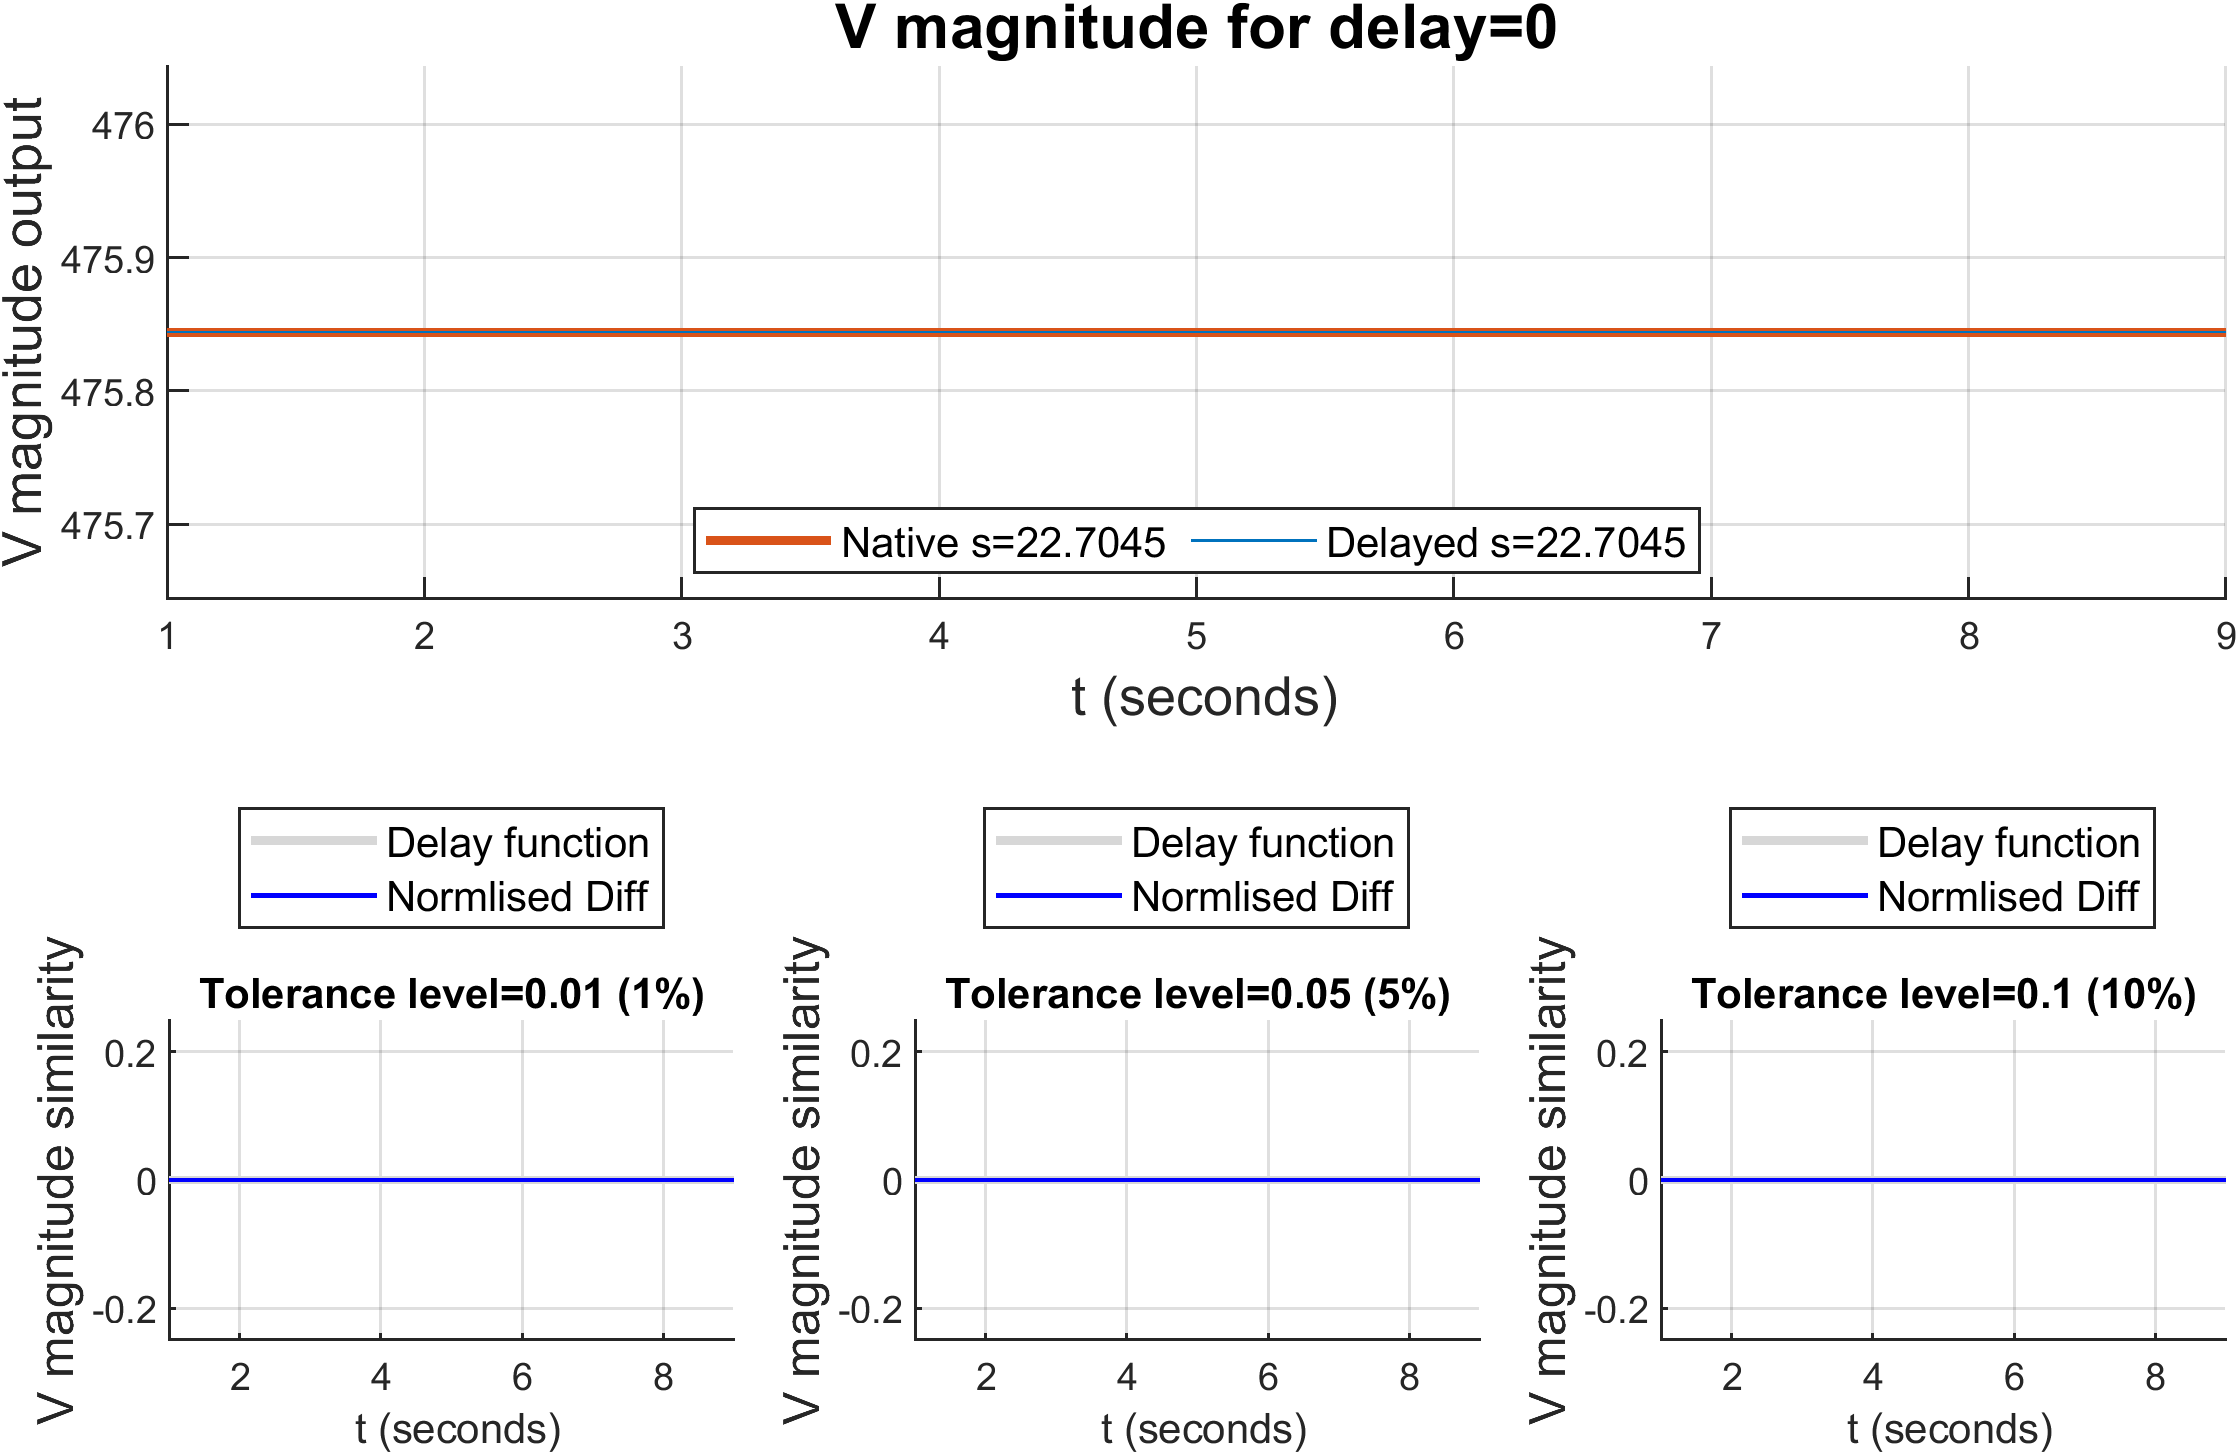
\includegraphics[width=0.95\textwidth]{PMUsim-figures/DelayOf_0/Zero_vMagnitude.png}}\\
   \\ 
    \fbox{ 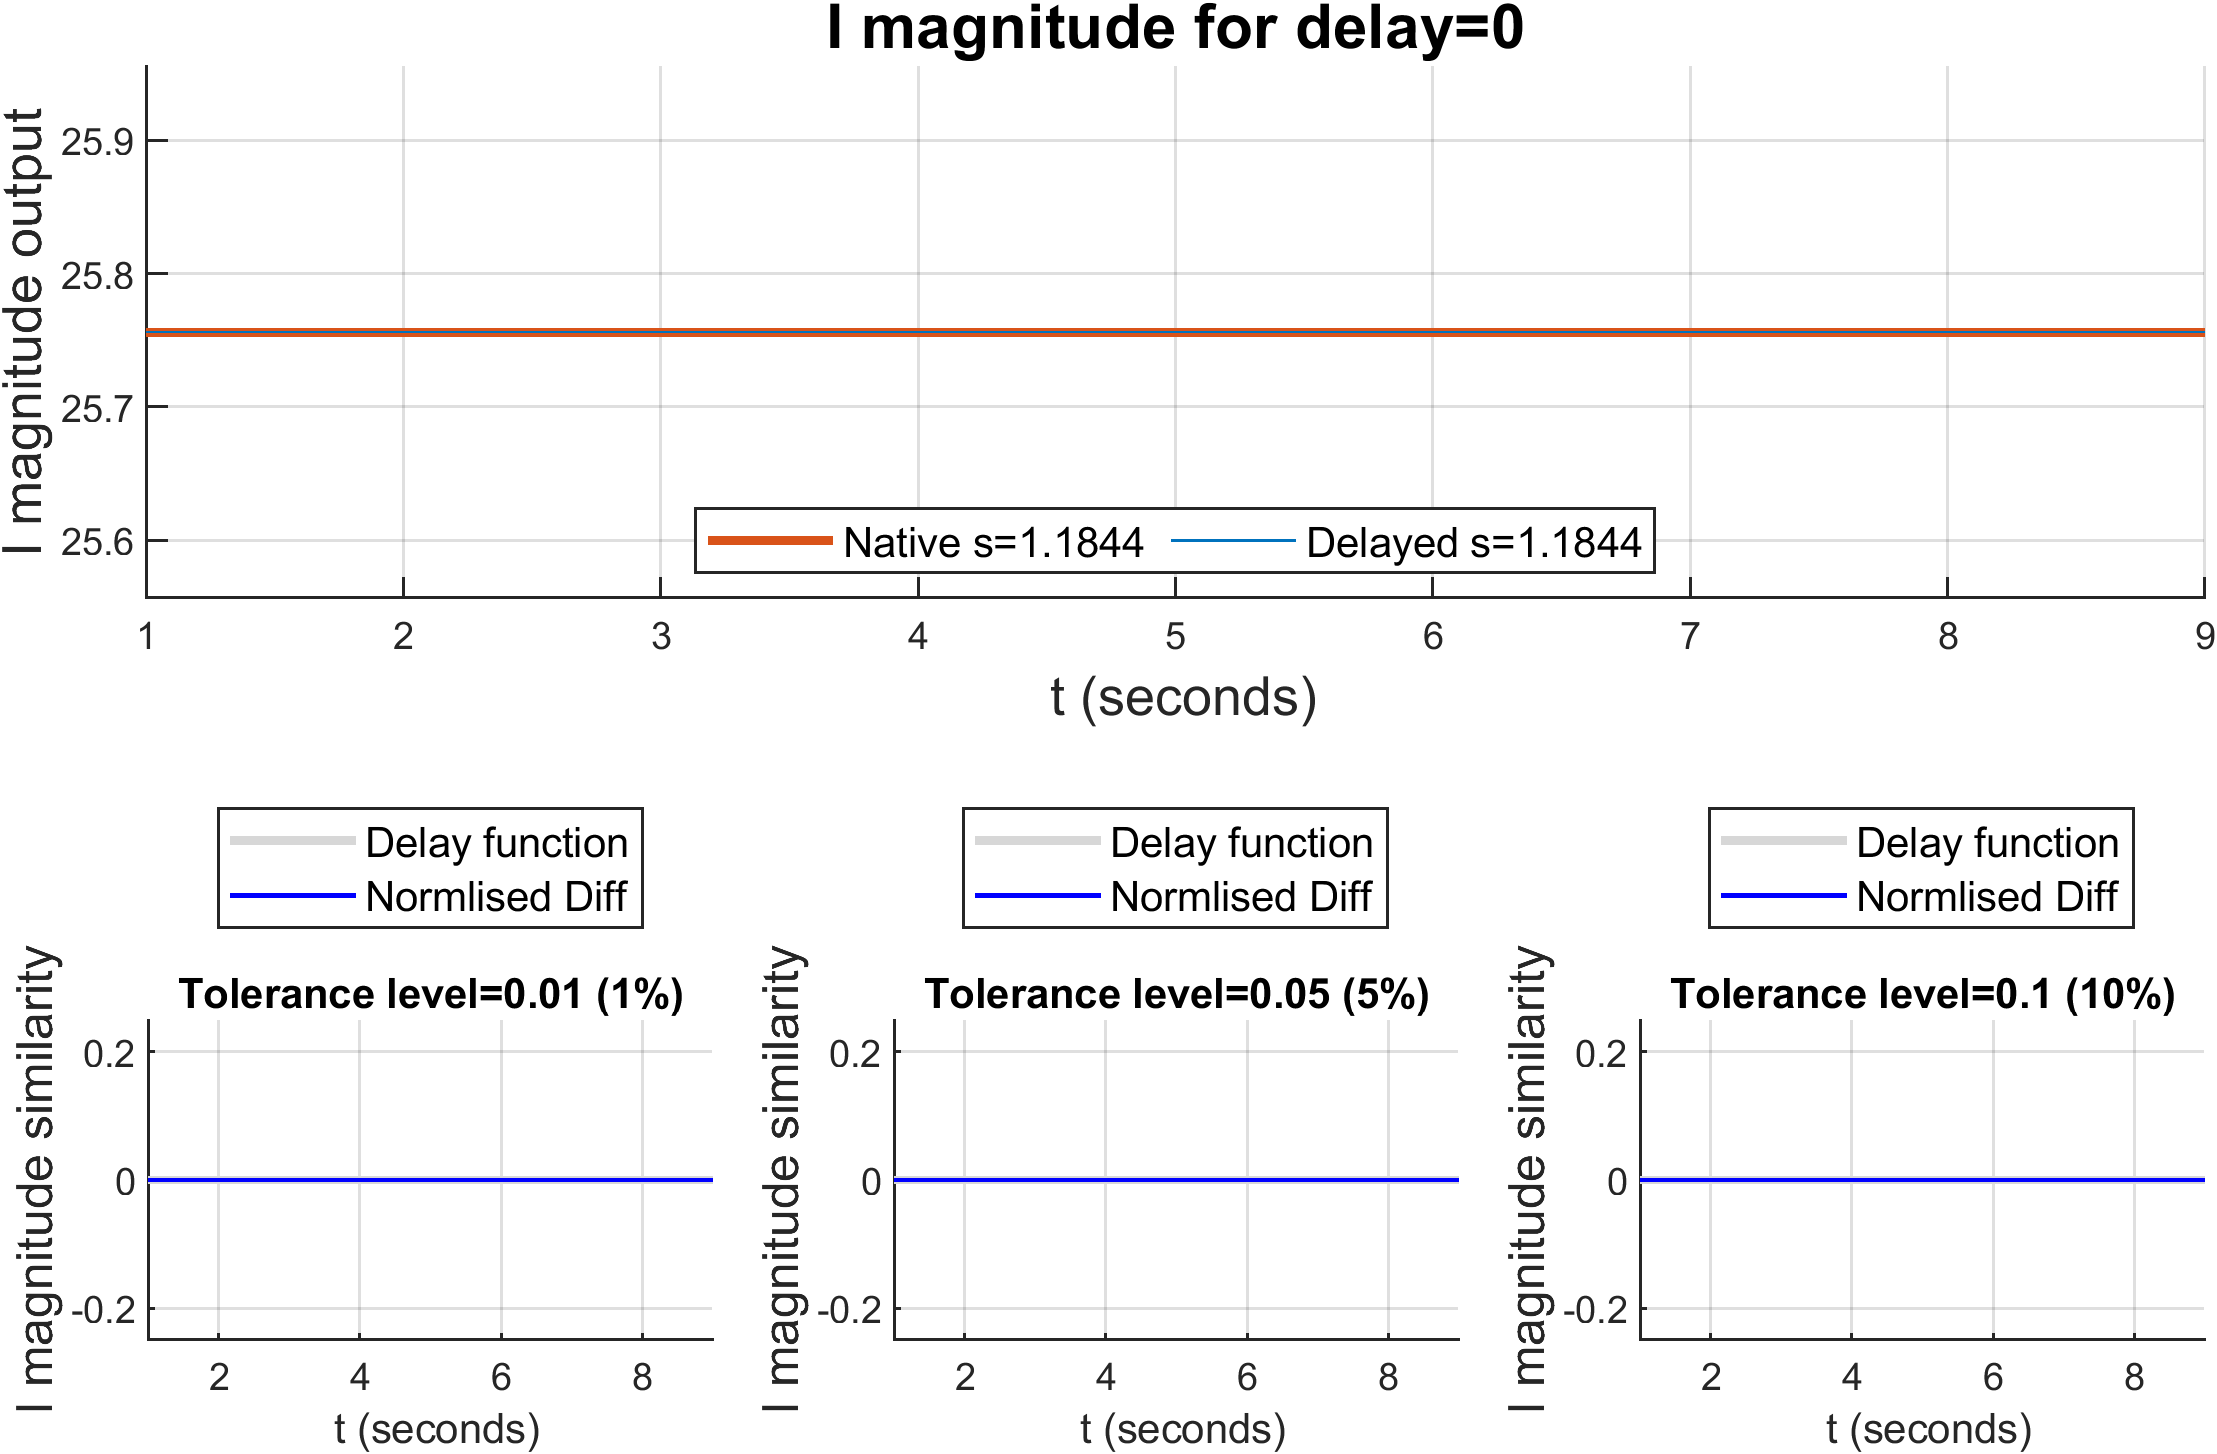
\includegraphics[width=0.95\textwidth]{PMUsim-figures/DelayOf_0/Zero_iMagnitude.png}}
  \end{tabular}
\caption{Results for Magnitude Output for Delay equal to Zero }
\end{figure}






  
  


\newpage
\begin{figure}[H]
\begin{tabular}{c}
   \fbox{    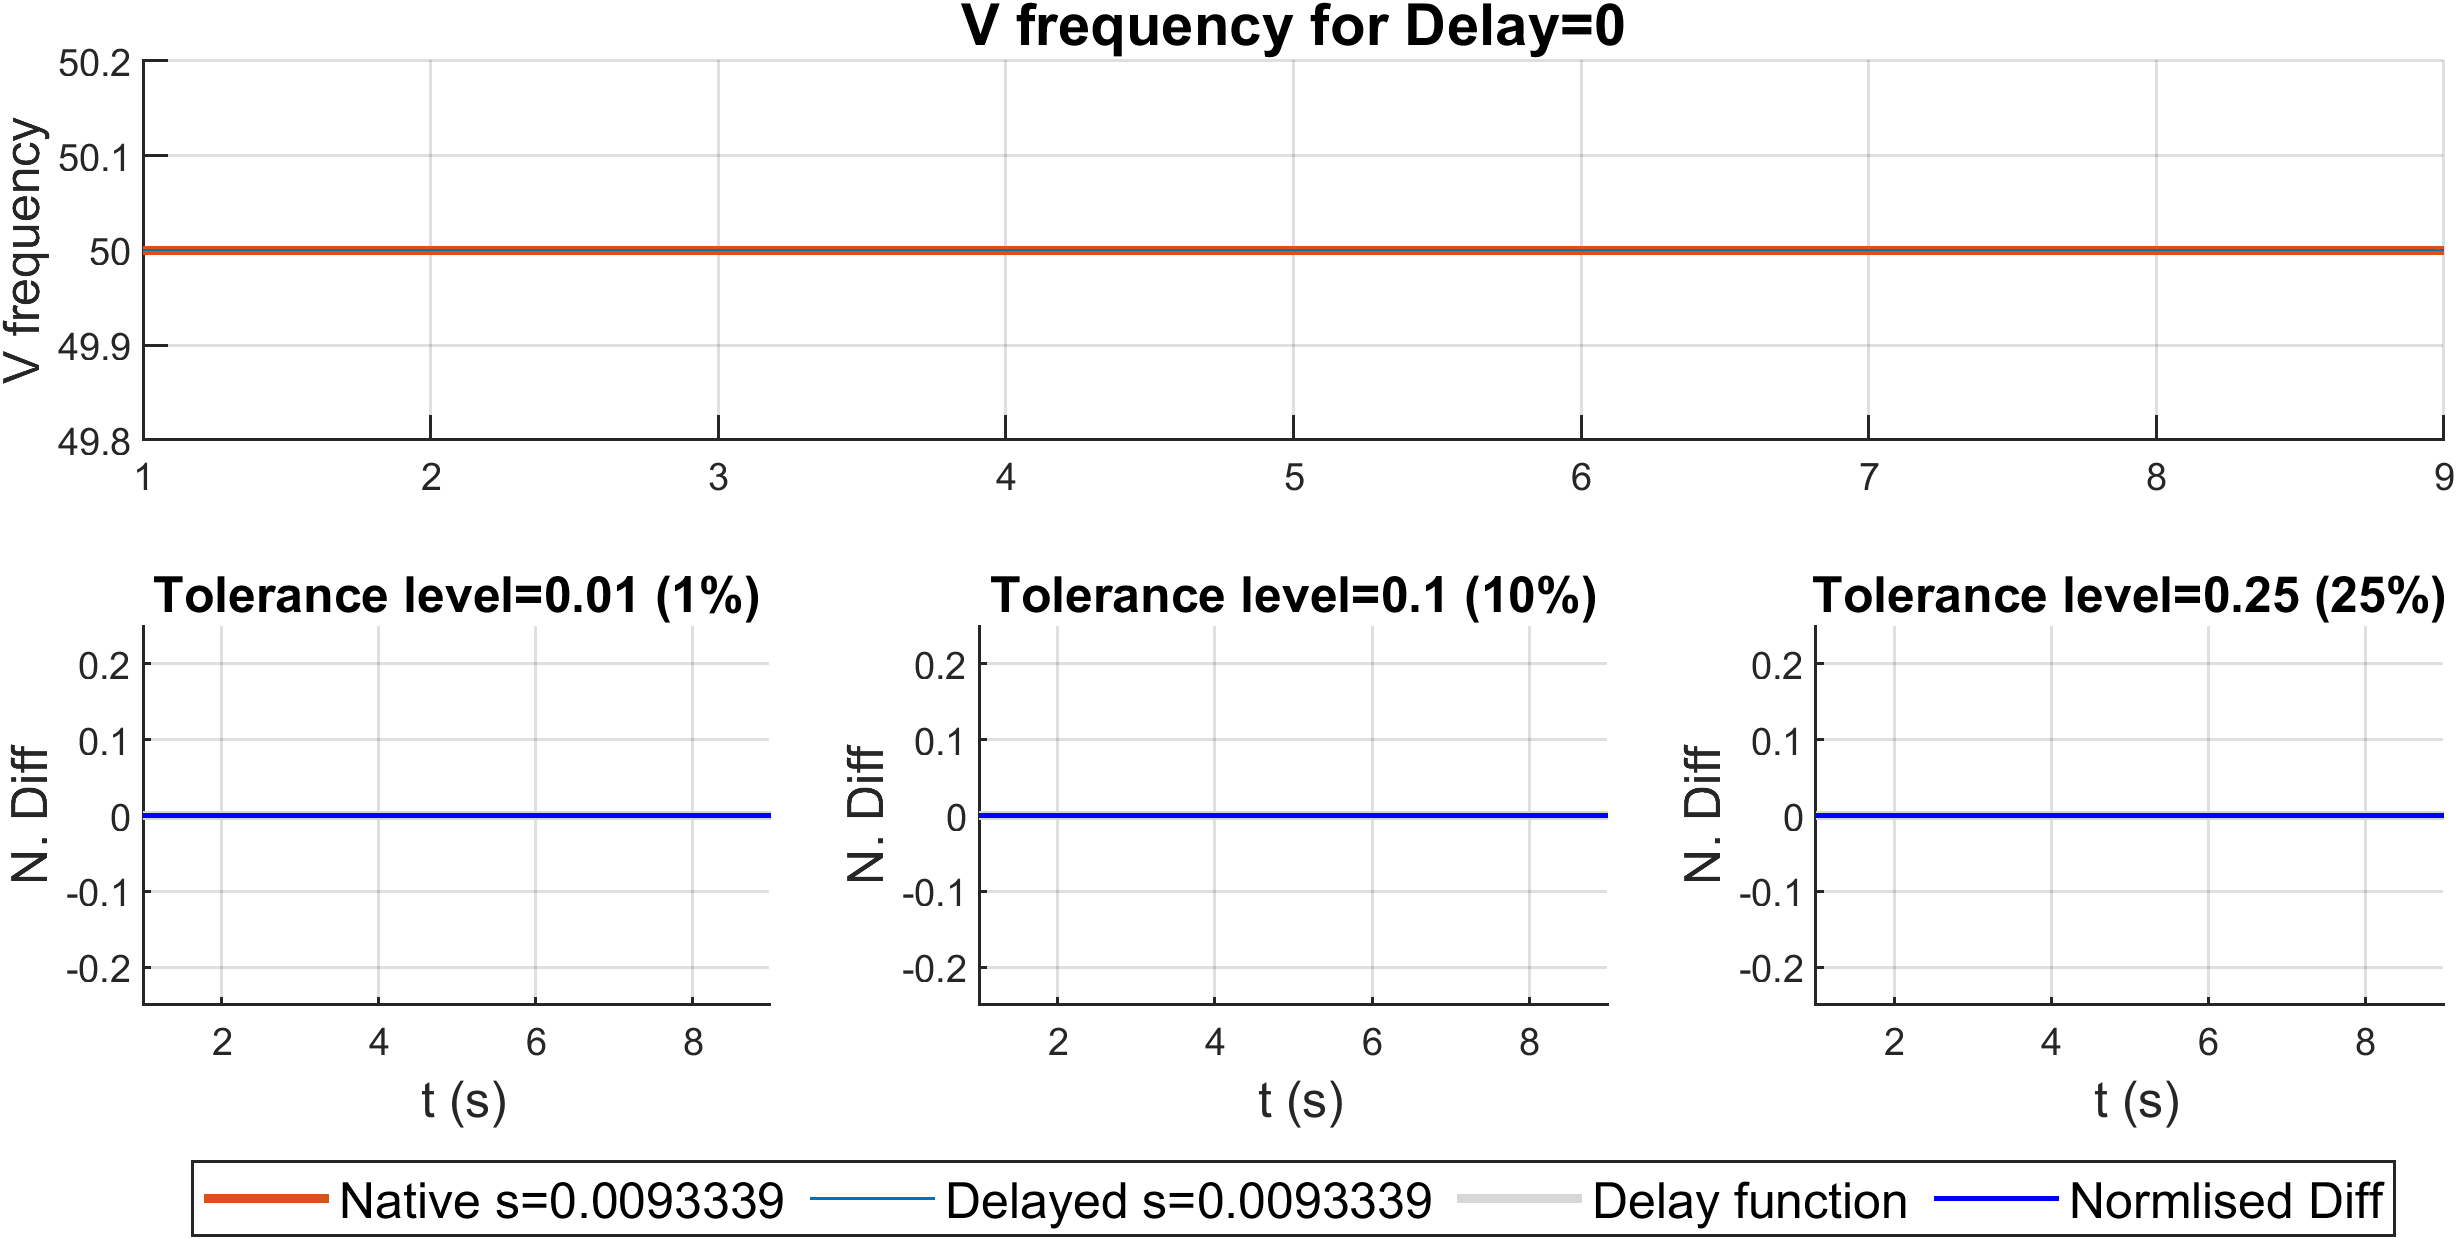
\includegraphics[width=0.95\textwidth]{PMUsim-figures/DelayOf_0/Zero_vFrequency.png}}\\
  \\ 
       \fbox{ 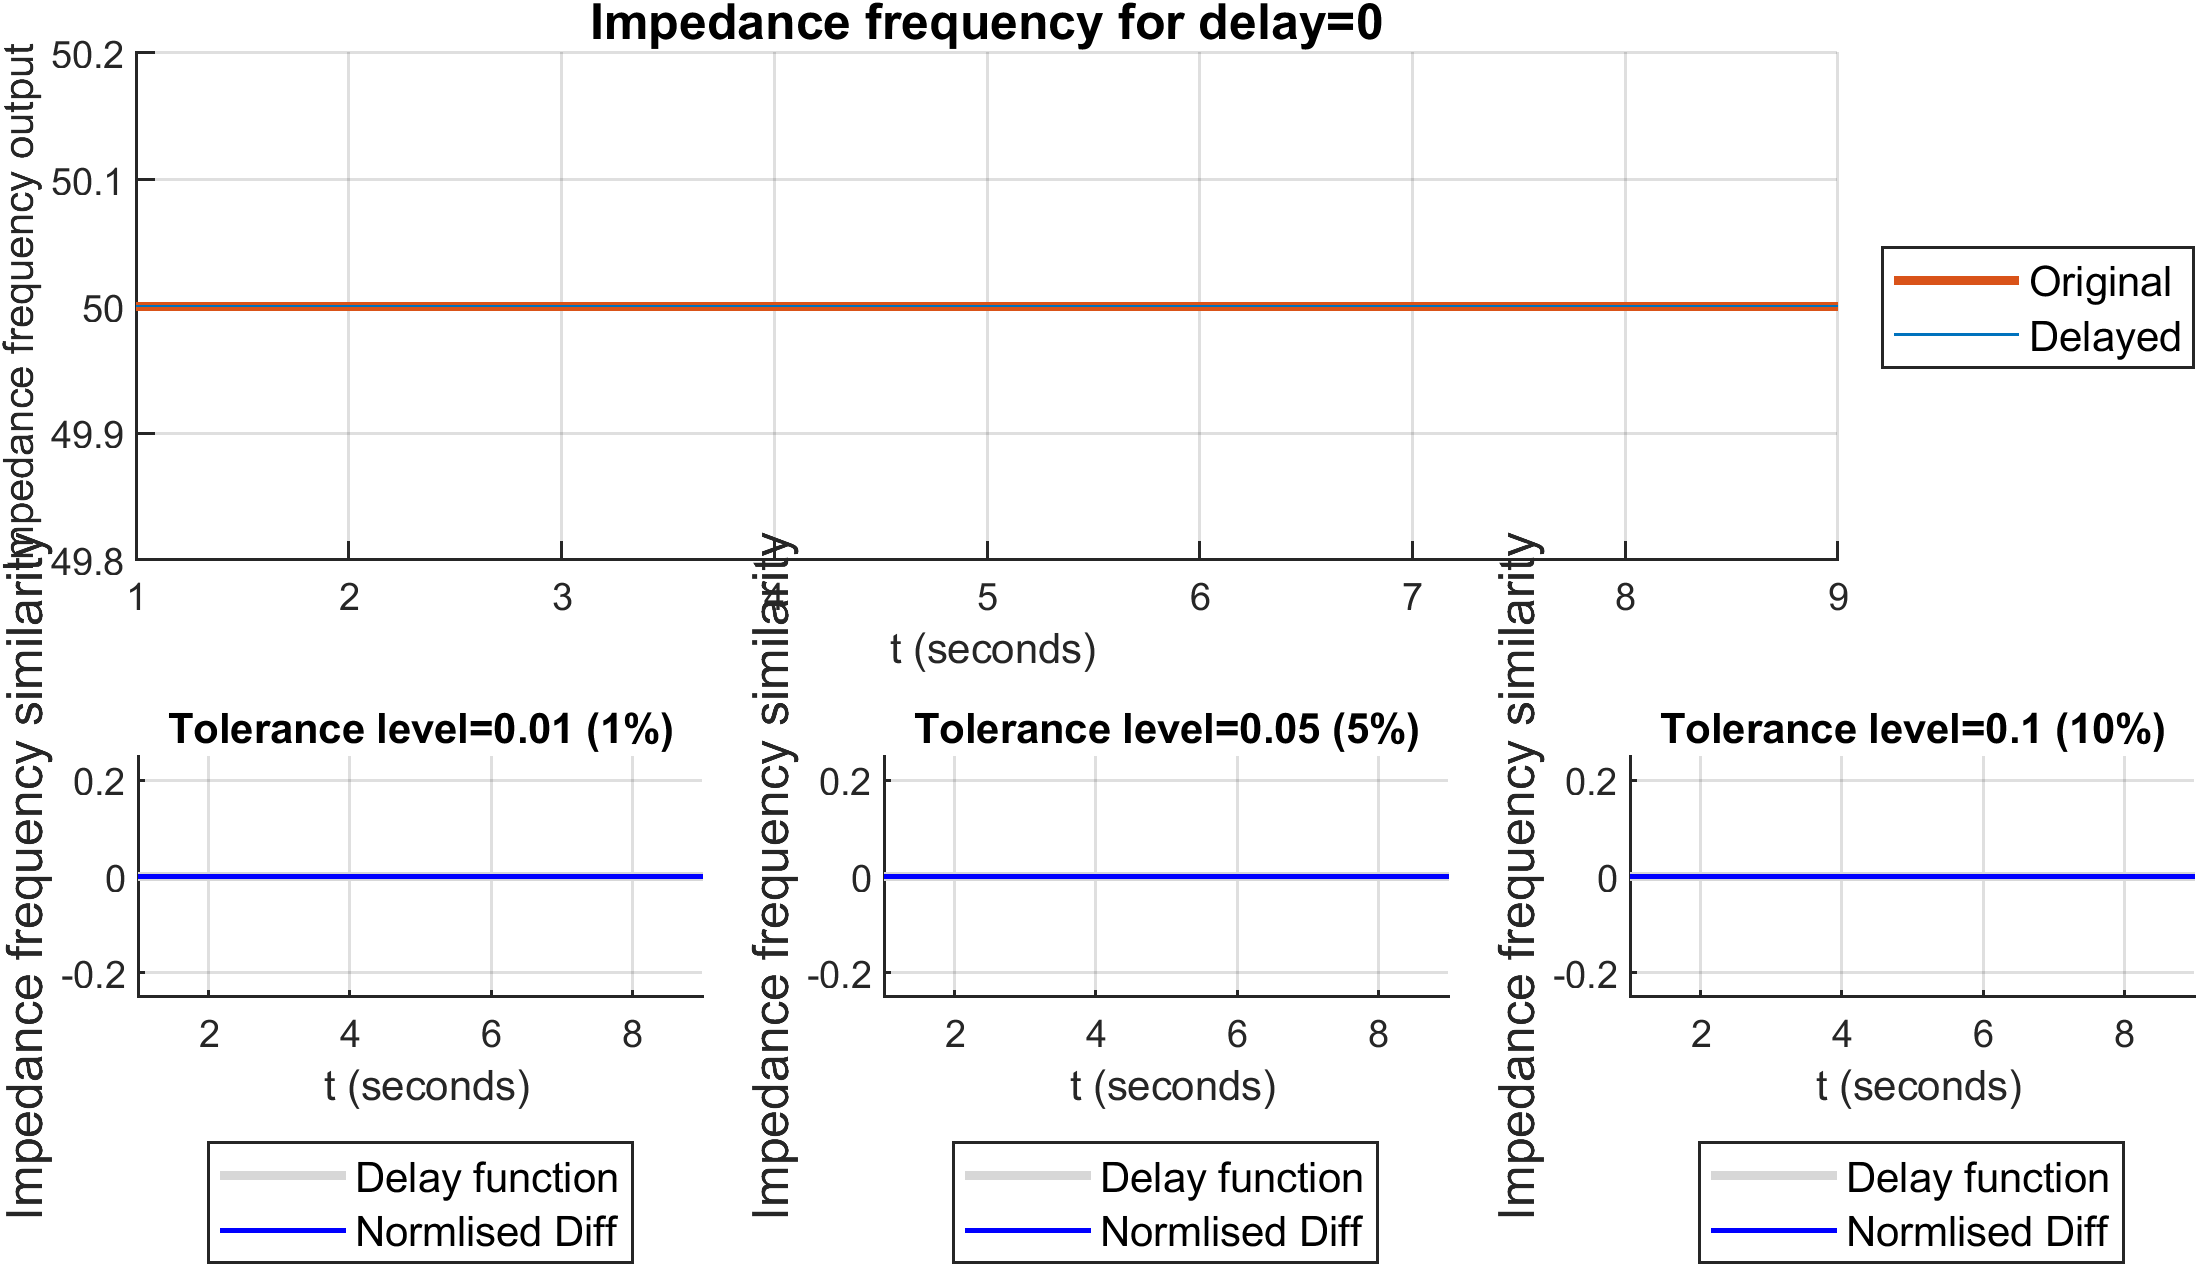
\includegraphics[width=0.95\textwidth]{PMUsim-figures/DelayOf_0/Zero_iFrequency.png}}
 \label{fig:PMUsim_Zero_Freq}
 %\caption{Zero Delay Frequency Output (for the Delay Level of Zero)}
  \end{tabular}
\caption{Results for Frequency Output for Delay equal to Zero }
\end{figure}




\newpage
\begin{figure}[H]
\begin{tabular}{c}
   \fbox{     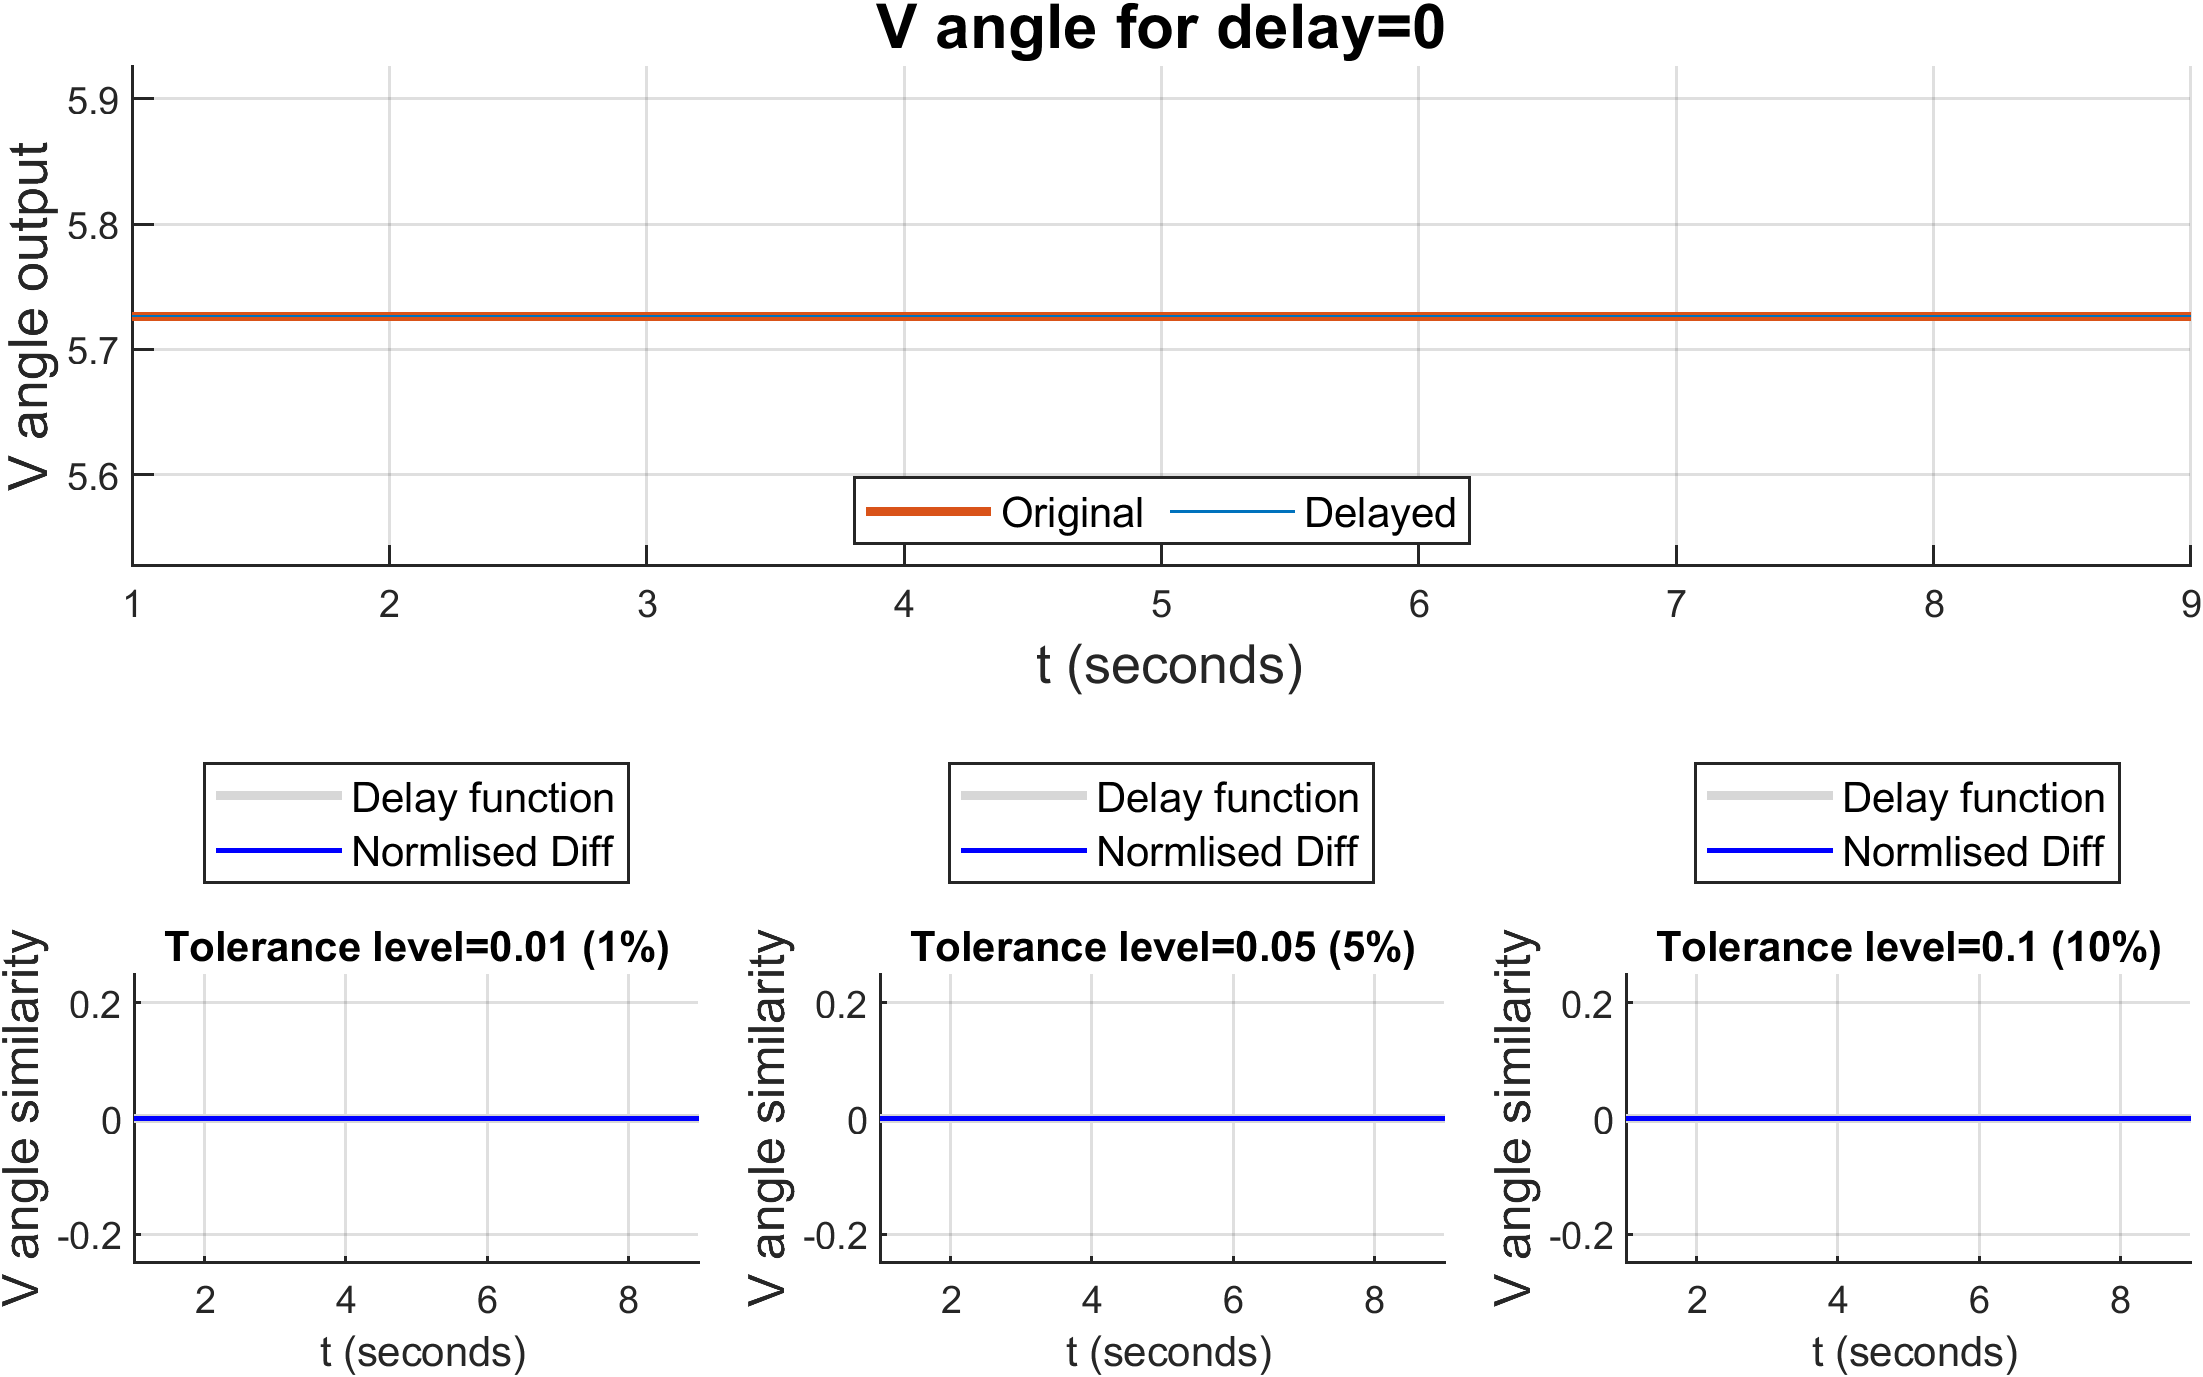
\includegraphics[width=0.95\textwidth]{PMUsim-figures/DelayOf_0/Zero_vAngle.png}}\\
  \\ 
   
   \fbox{  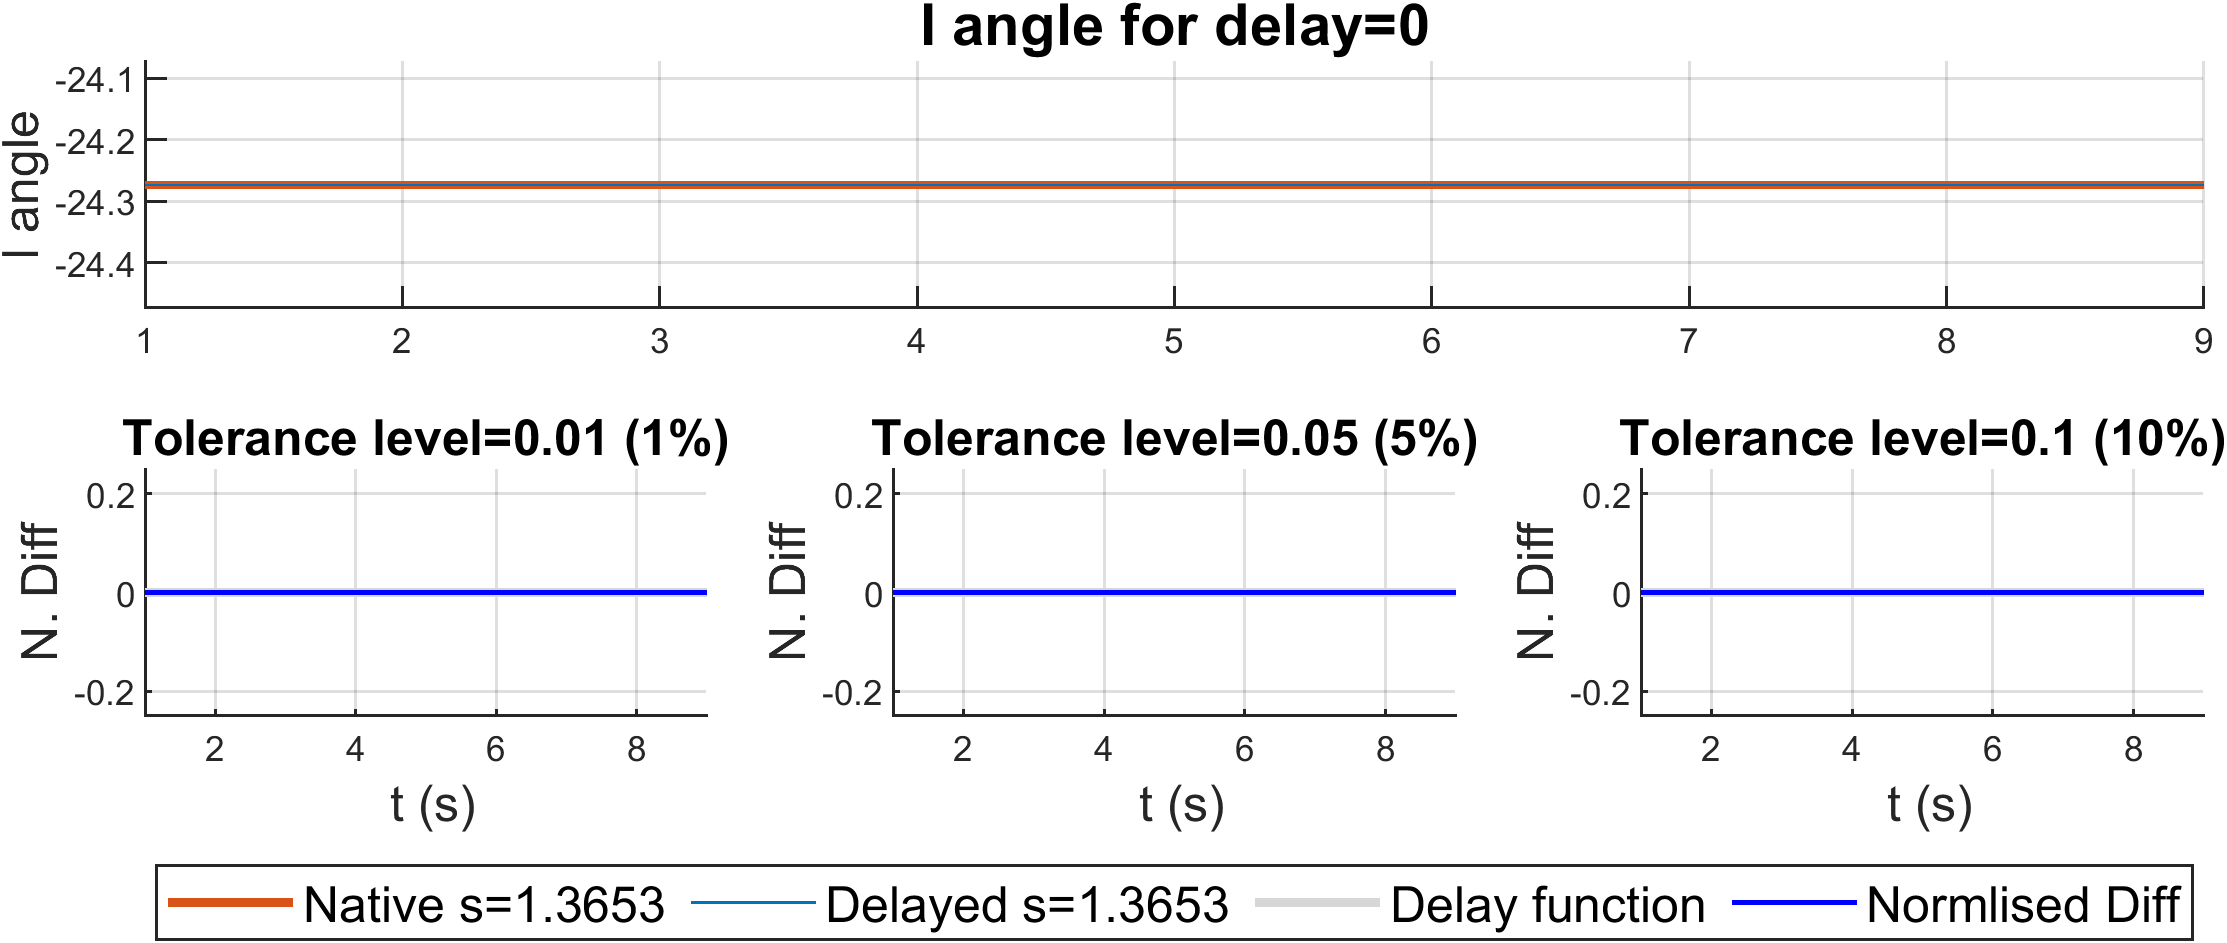
\includegraphics[width=0.95\textwidth]{PMUsim-figures/DelayOf_0/Zero_iAngle.png}}\\

     \label{fig:PMUsim_Zero_Angle}
     %\caption{Zero Delay Angle Output (for the Delay Level of Zero)}
  \end{tabular}
\caption{Results for Angle Output for Delay equal to Zero }
 \end{figure}
 \newpage
\section{Instant Delay Functions}

\subsection{Instant Delay Level of One}


\begin{small}
     \tcbox[size=normal, standard jigsaw, opacityback=0, boxrule=0pt,halign=justify]{
     Instant Delay Level of One}{
          \begin{itemize}
         \item      The delayed signal (blue) overlaps the original signal (red), producing a straight line, colored neither red nor blue.
         \item  The blue Normalised diff signal also overlaps the grey delay function.
          \end{itemize} }
\end{small}



\newpage
\begin{figure}[H]
\begin{tabular}{c}
   \fbox{     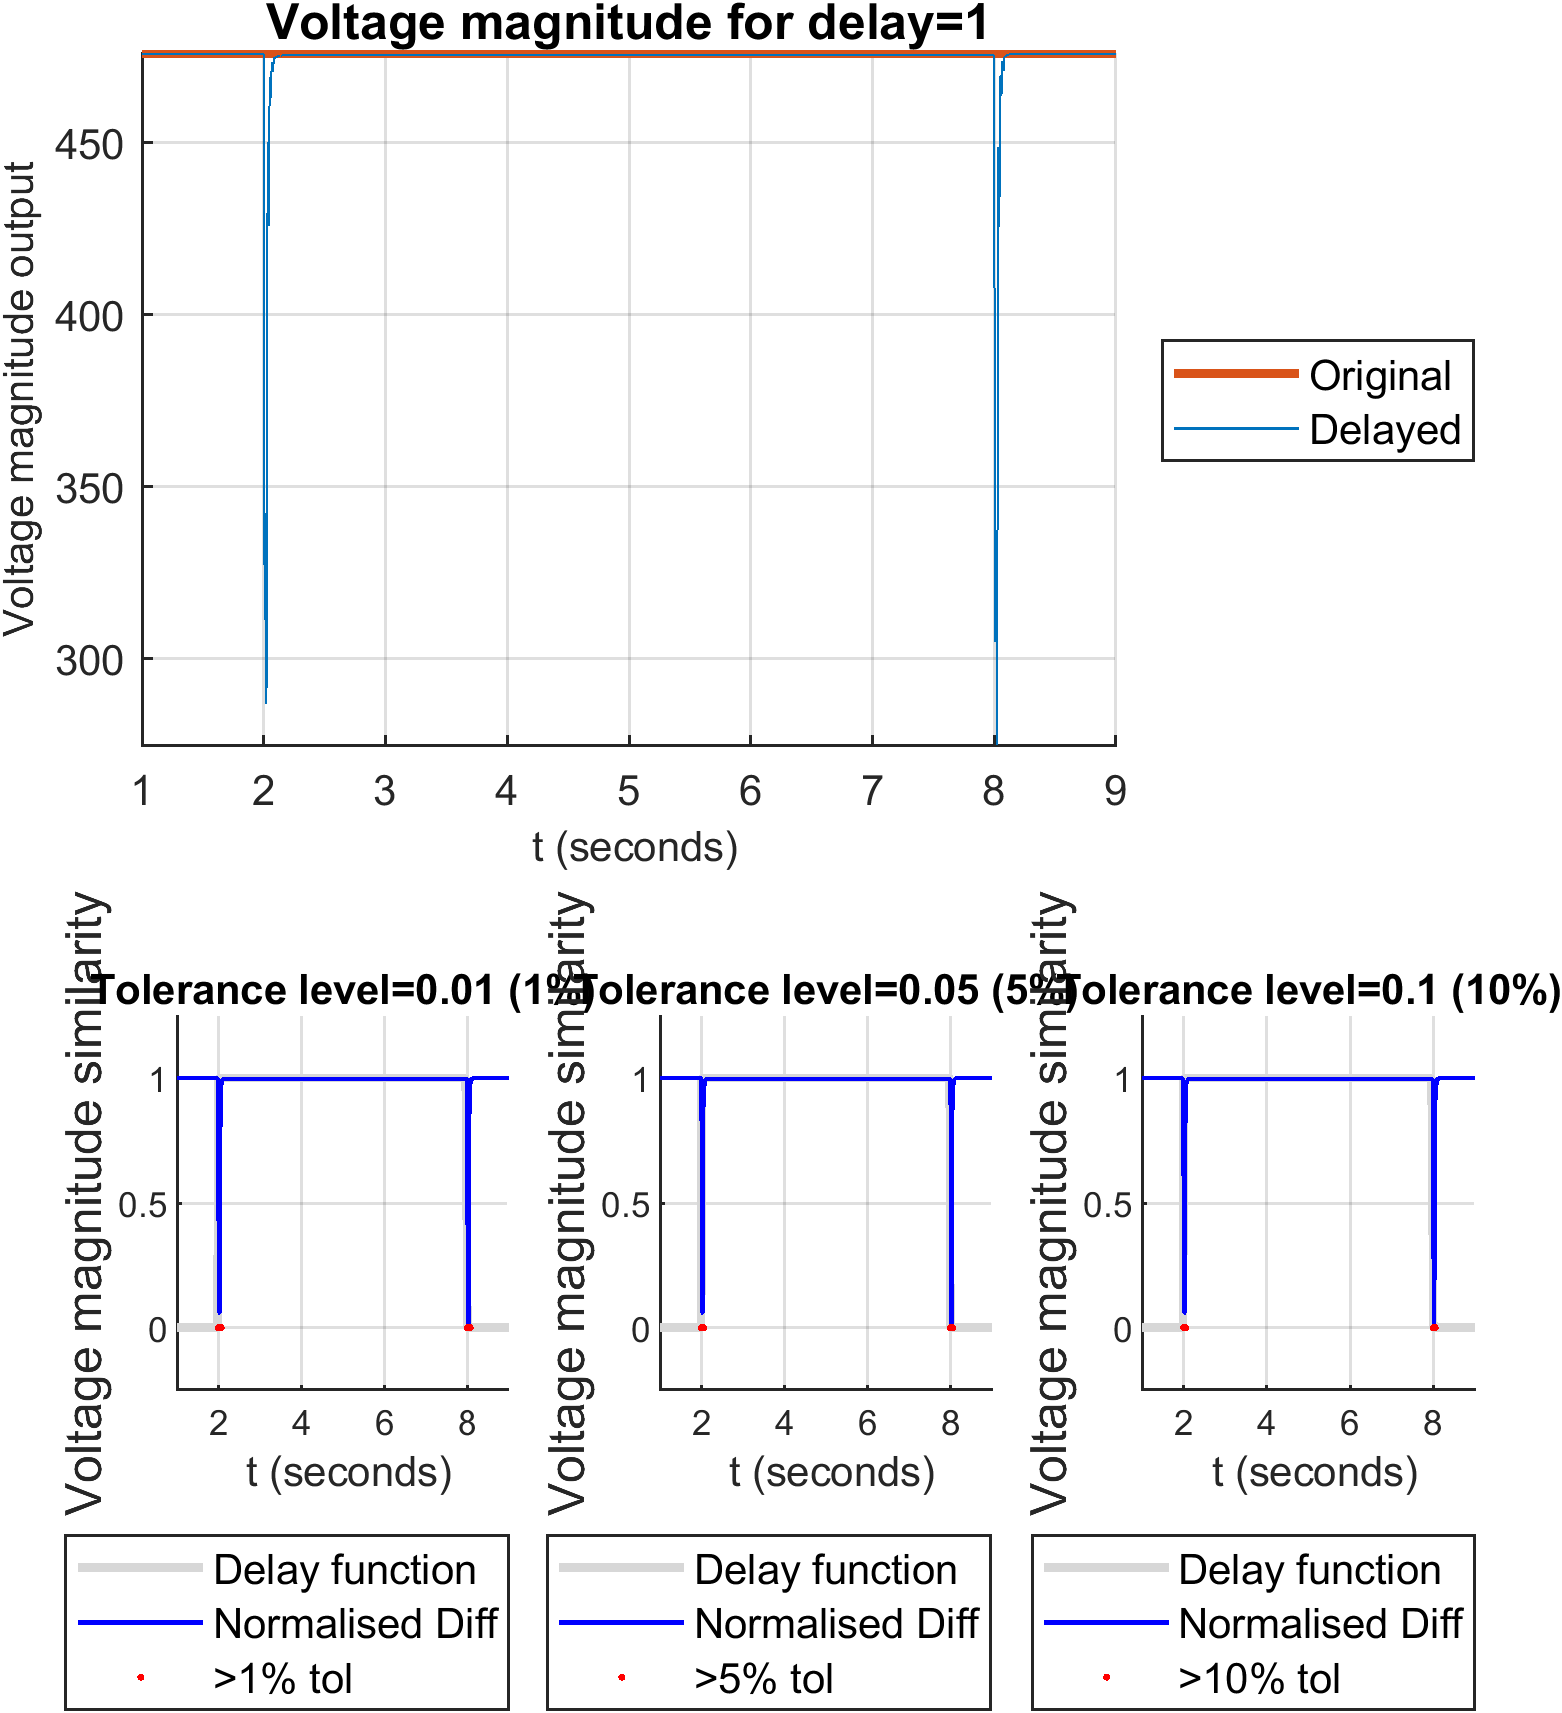
\includegraphics[width=0.95\textwidth]{PMUsim-figures/DelayOf_1/Instant_vMagnitude.png}}\\
    \\ 
    
   \fbox{  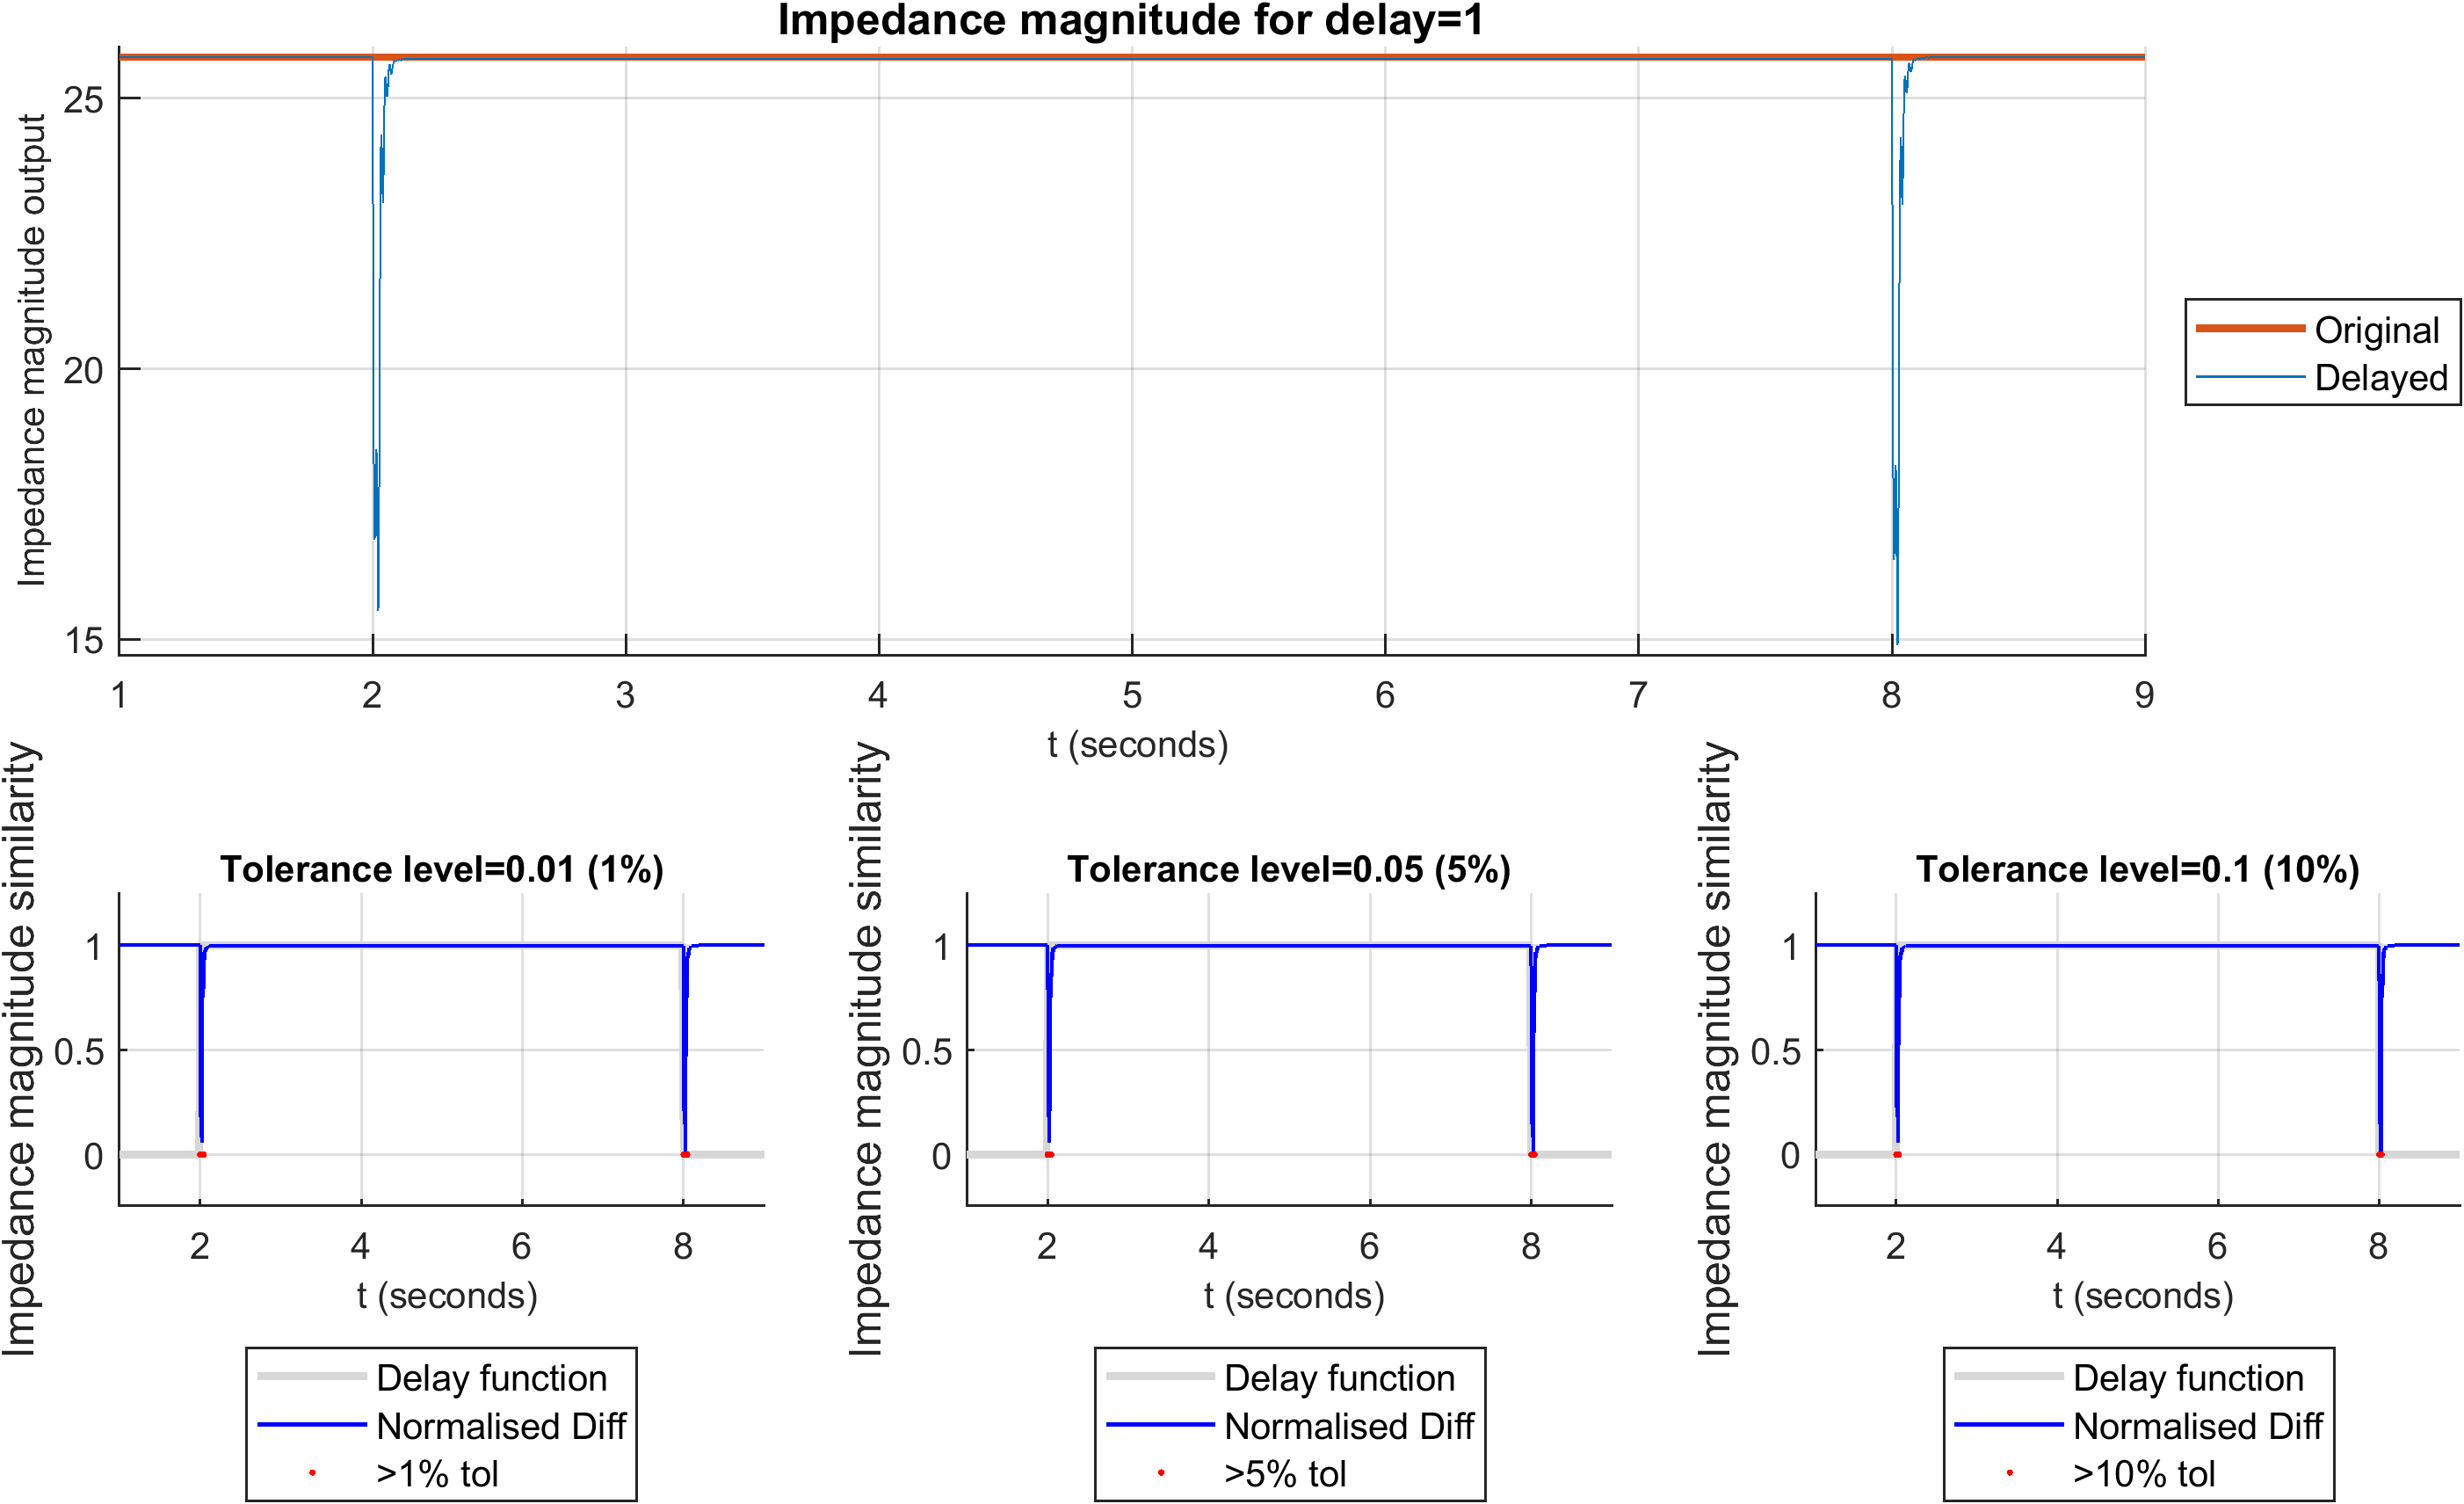
\includegraphics[width=0.95\textwidth]{PMUsim-figures/DelayOf_1/Instant_iMagnitude.png}}   
 %\caption{Instant Delay Magnitude Output for the Delay Level of One}
  \end{tabular}
 \label{fig:pmuOneMag}
\caption[Instant delay of 1: Magnitude Output]{Results for Magnitude Output for Delay equal to One}
 \end{figure}
 \newpage
\begin{figure}[H]
\begin{tabular}{c}
  
   \fbox{  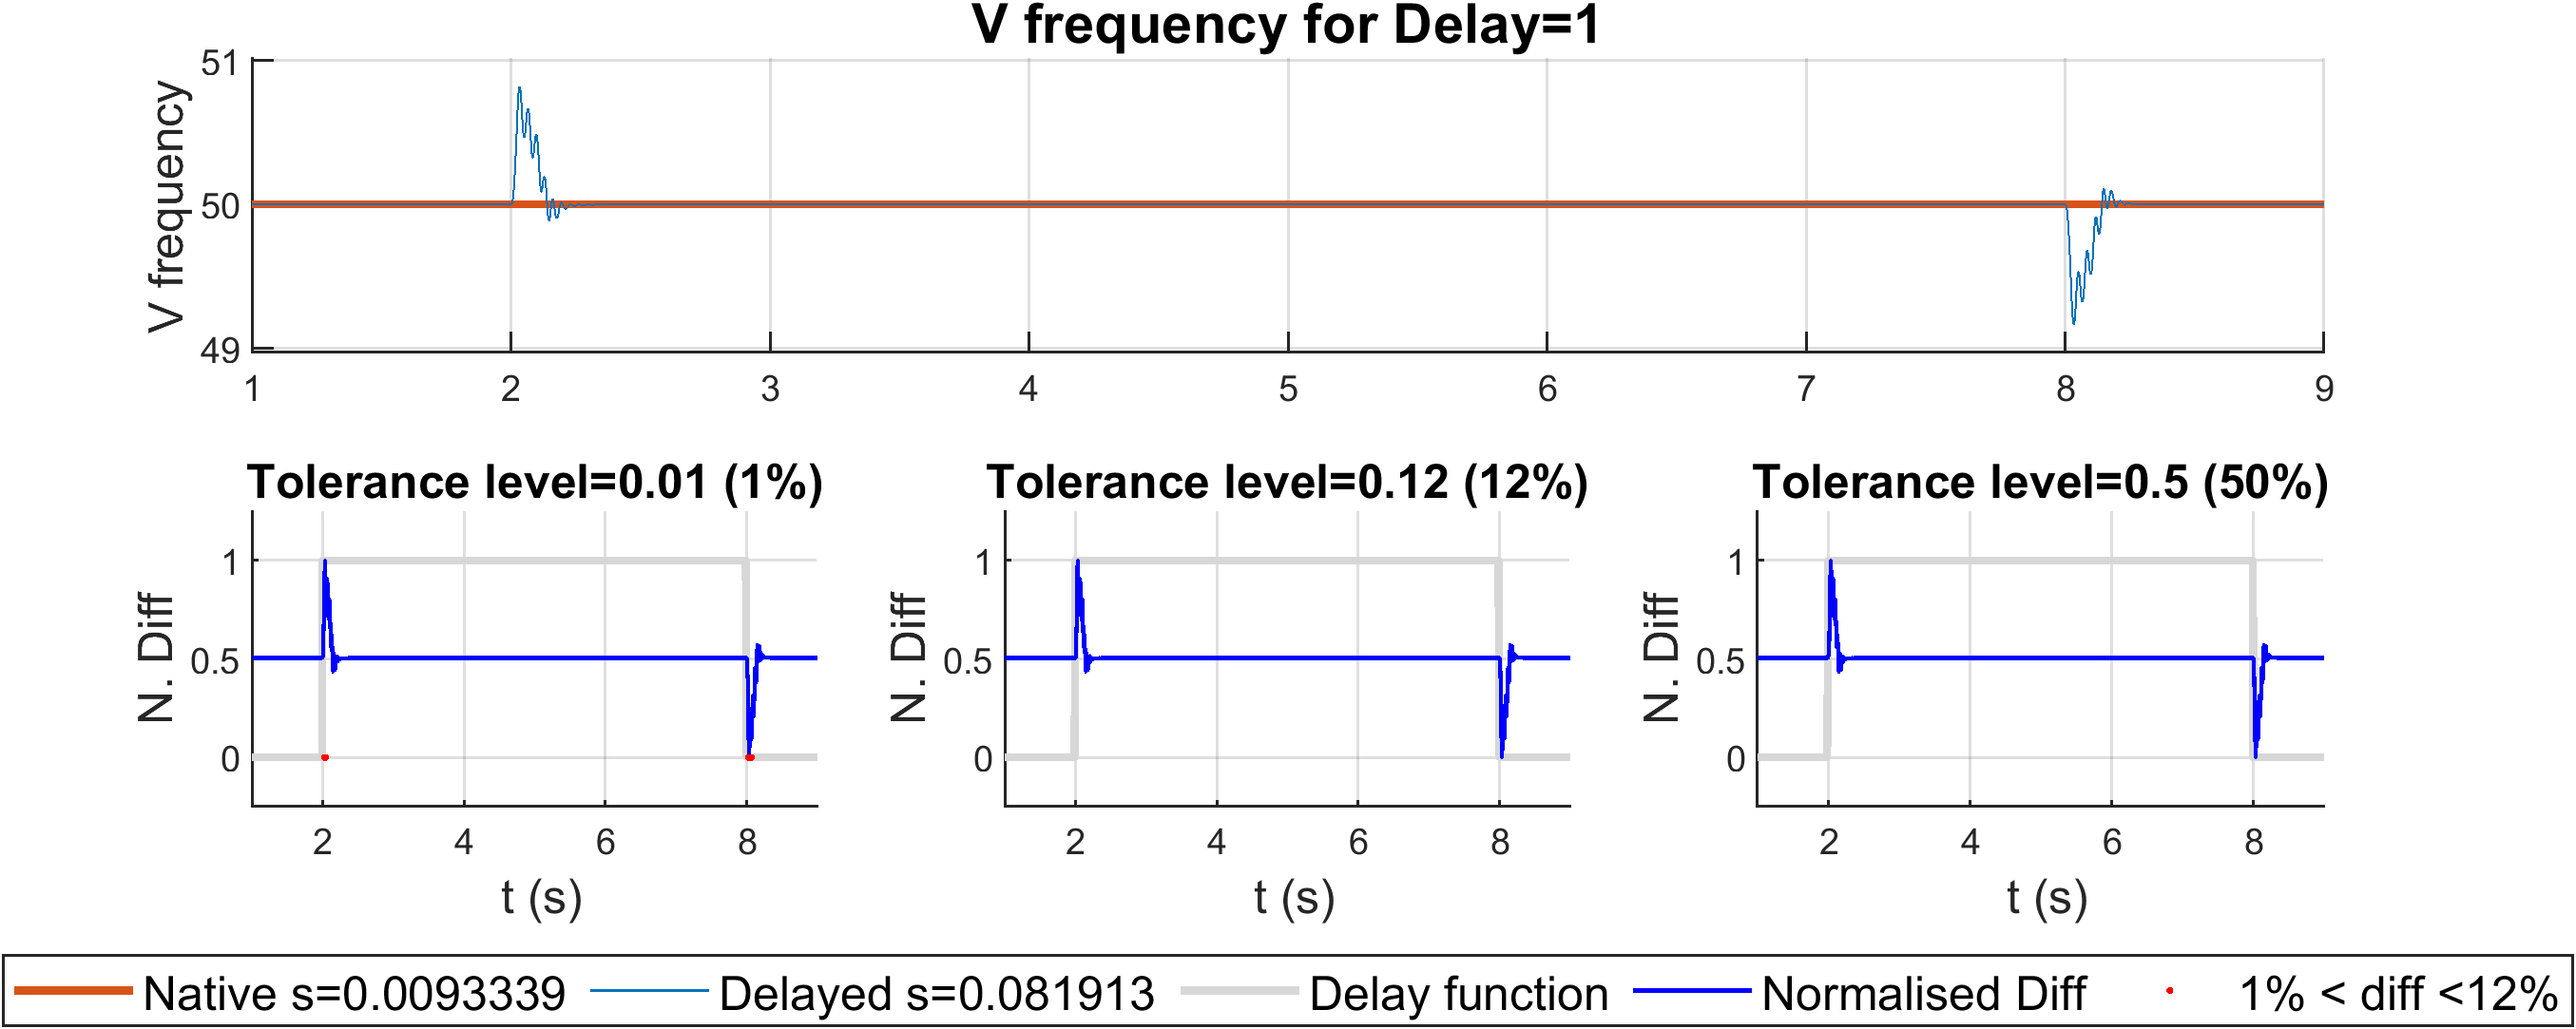
\includegraphics[width=0.95\textwidth]{PMUsim-figures/DelayOf_1/Instant_vFrequency.png}}\\
  
      \\ 
   \fbox{  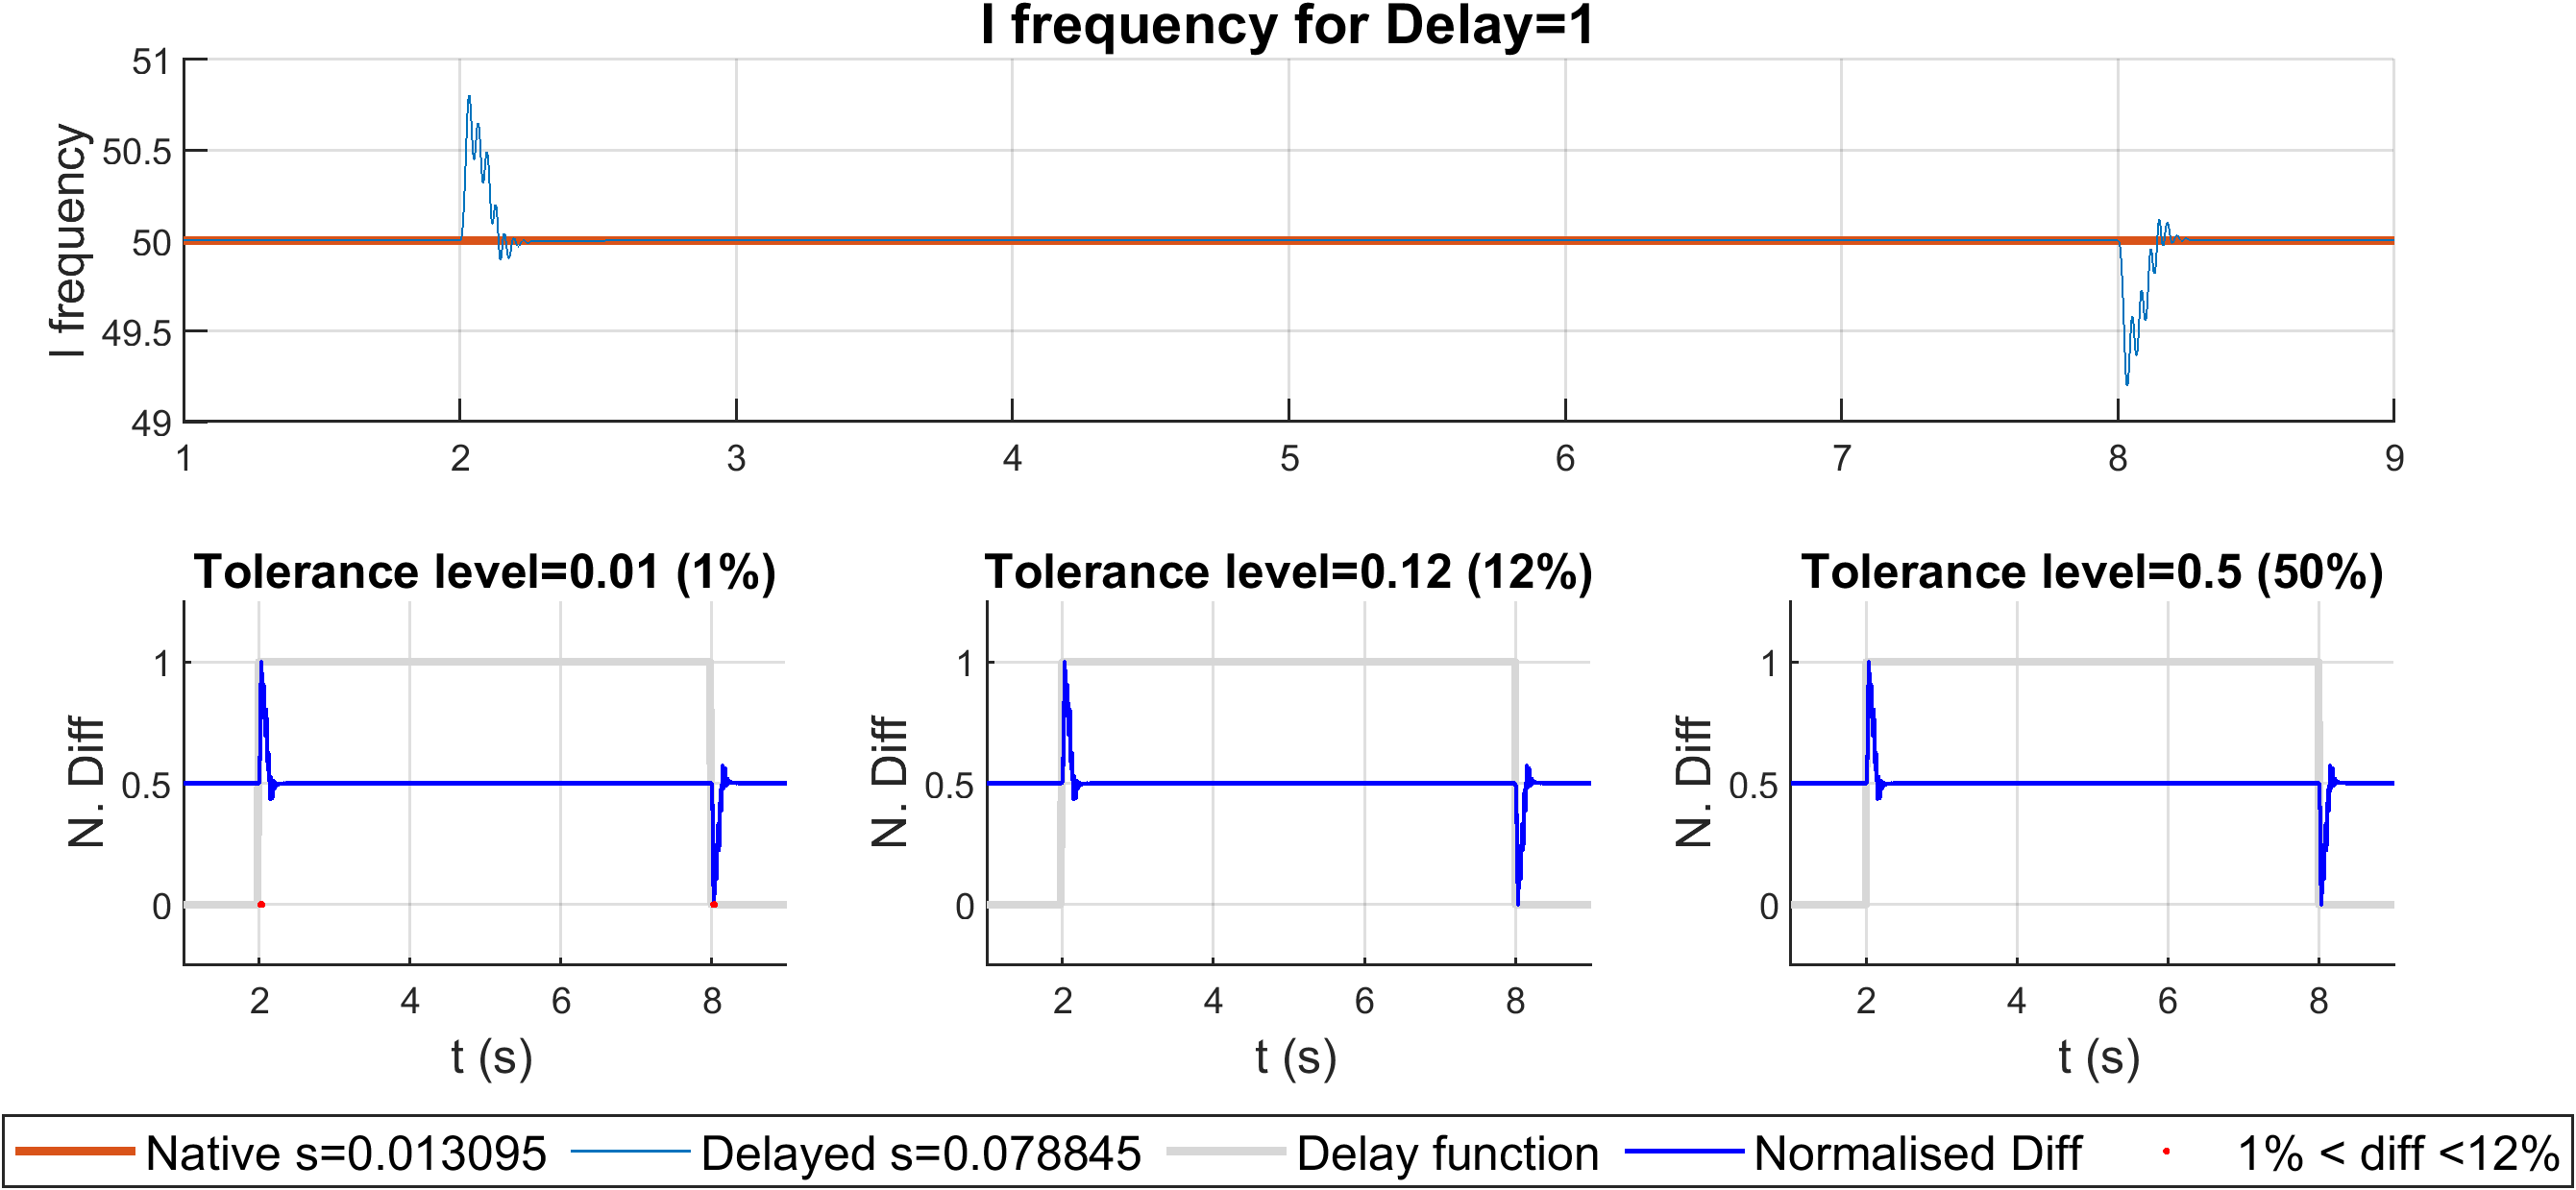
\includegraphics[width=0.95\textwidth]{PMUsim-figures/DelayOf_1/Instant_iFrequency.png}} 
 %\caption{Instant Delay Frequency Output for the Delay Level of One}
  \end{tabular}
\caption[Instant delay of 1: Frequency Output]{Results for Frequency Output for Delay equal to One}
 \label{fig:pmuOneFreq}
 \end{figure}



\newpage 
\begin{figure}[H]
\begin{tabular}{c}
   \fbox{    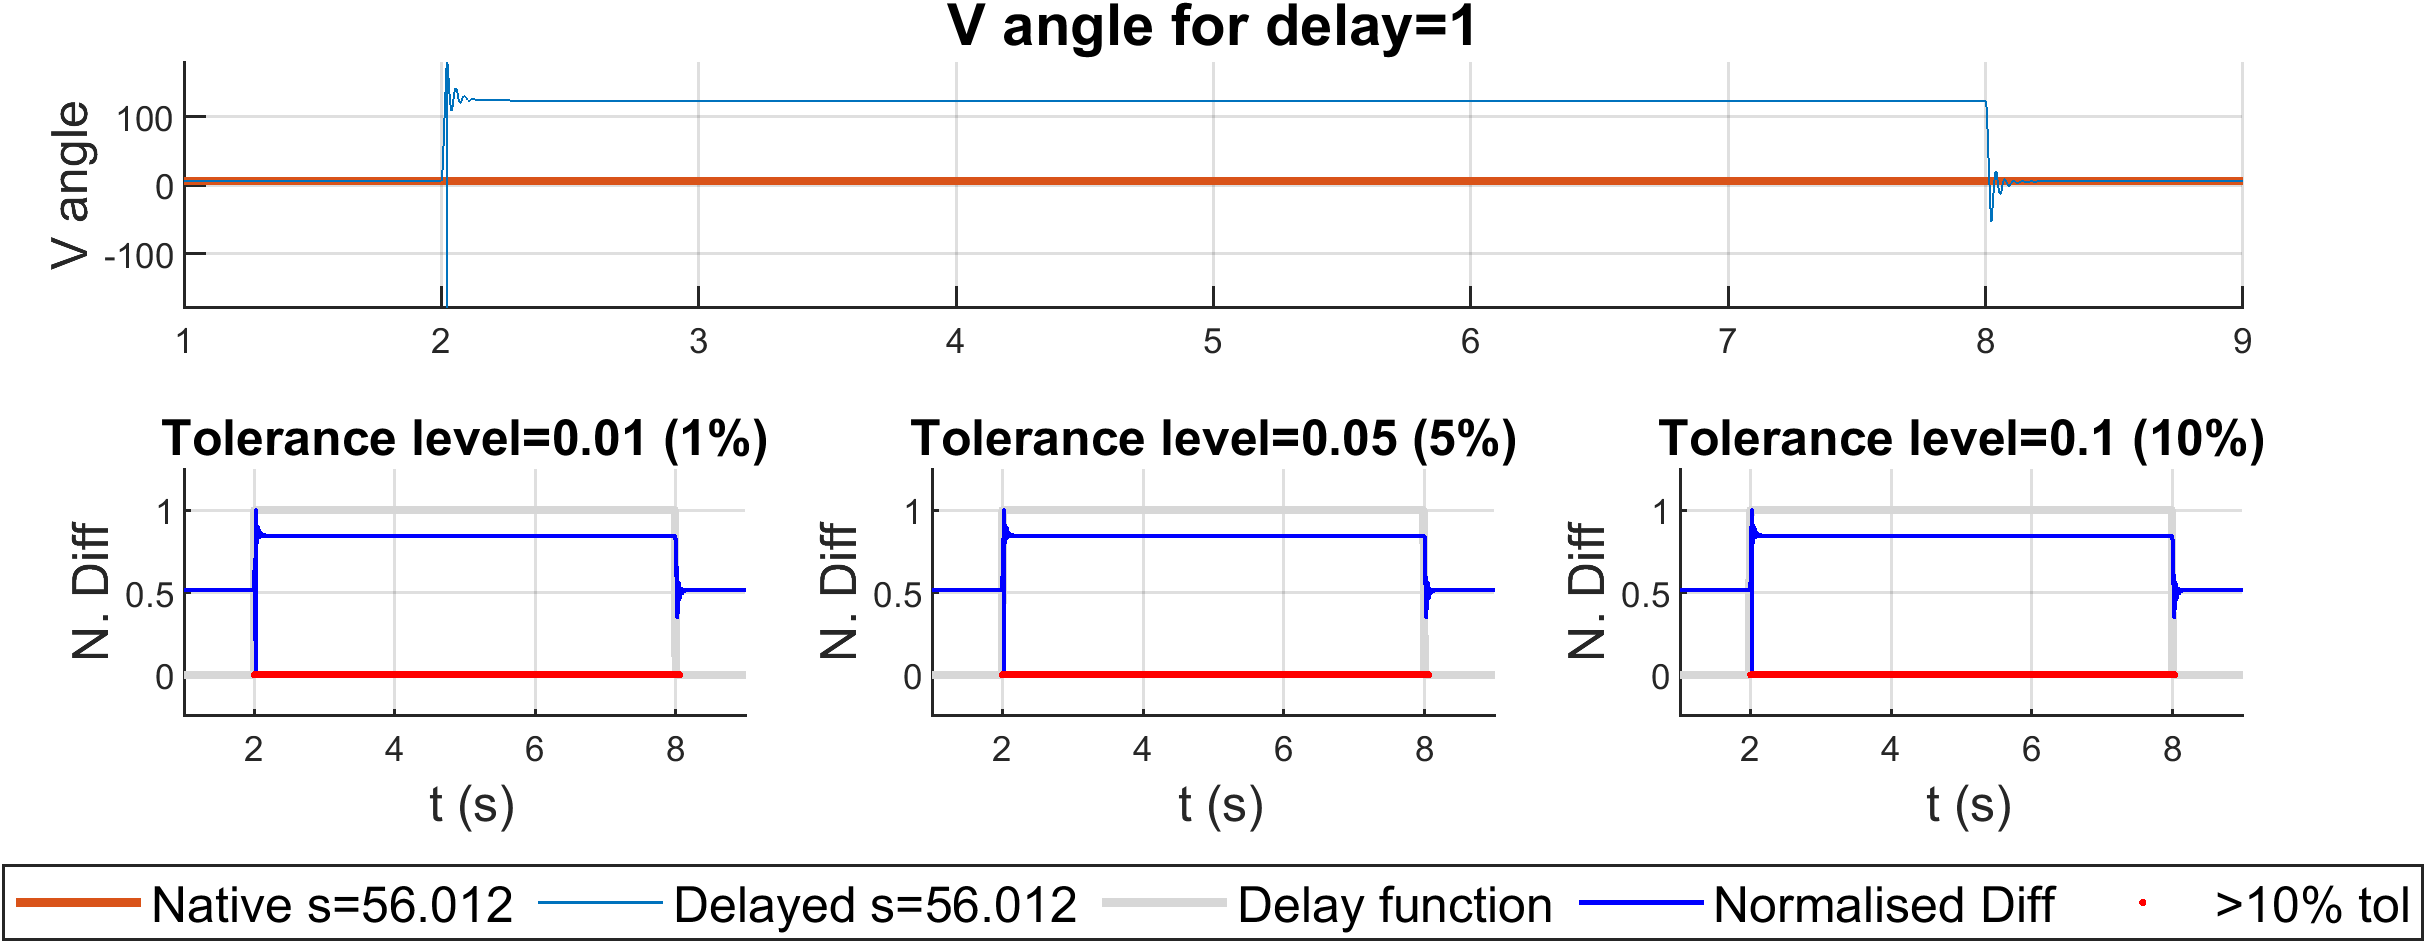
\includegraphics[width=0.95\textwidth]{PMUsim-figures/DelayOf_1/Instant_vAngle.png}}\\
    \\ 
    
   \fbox{  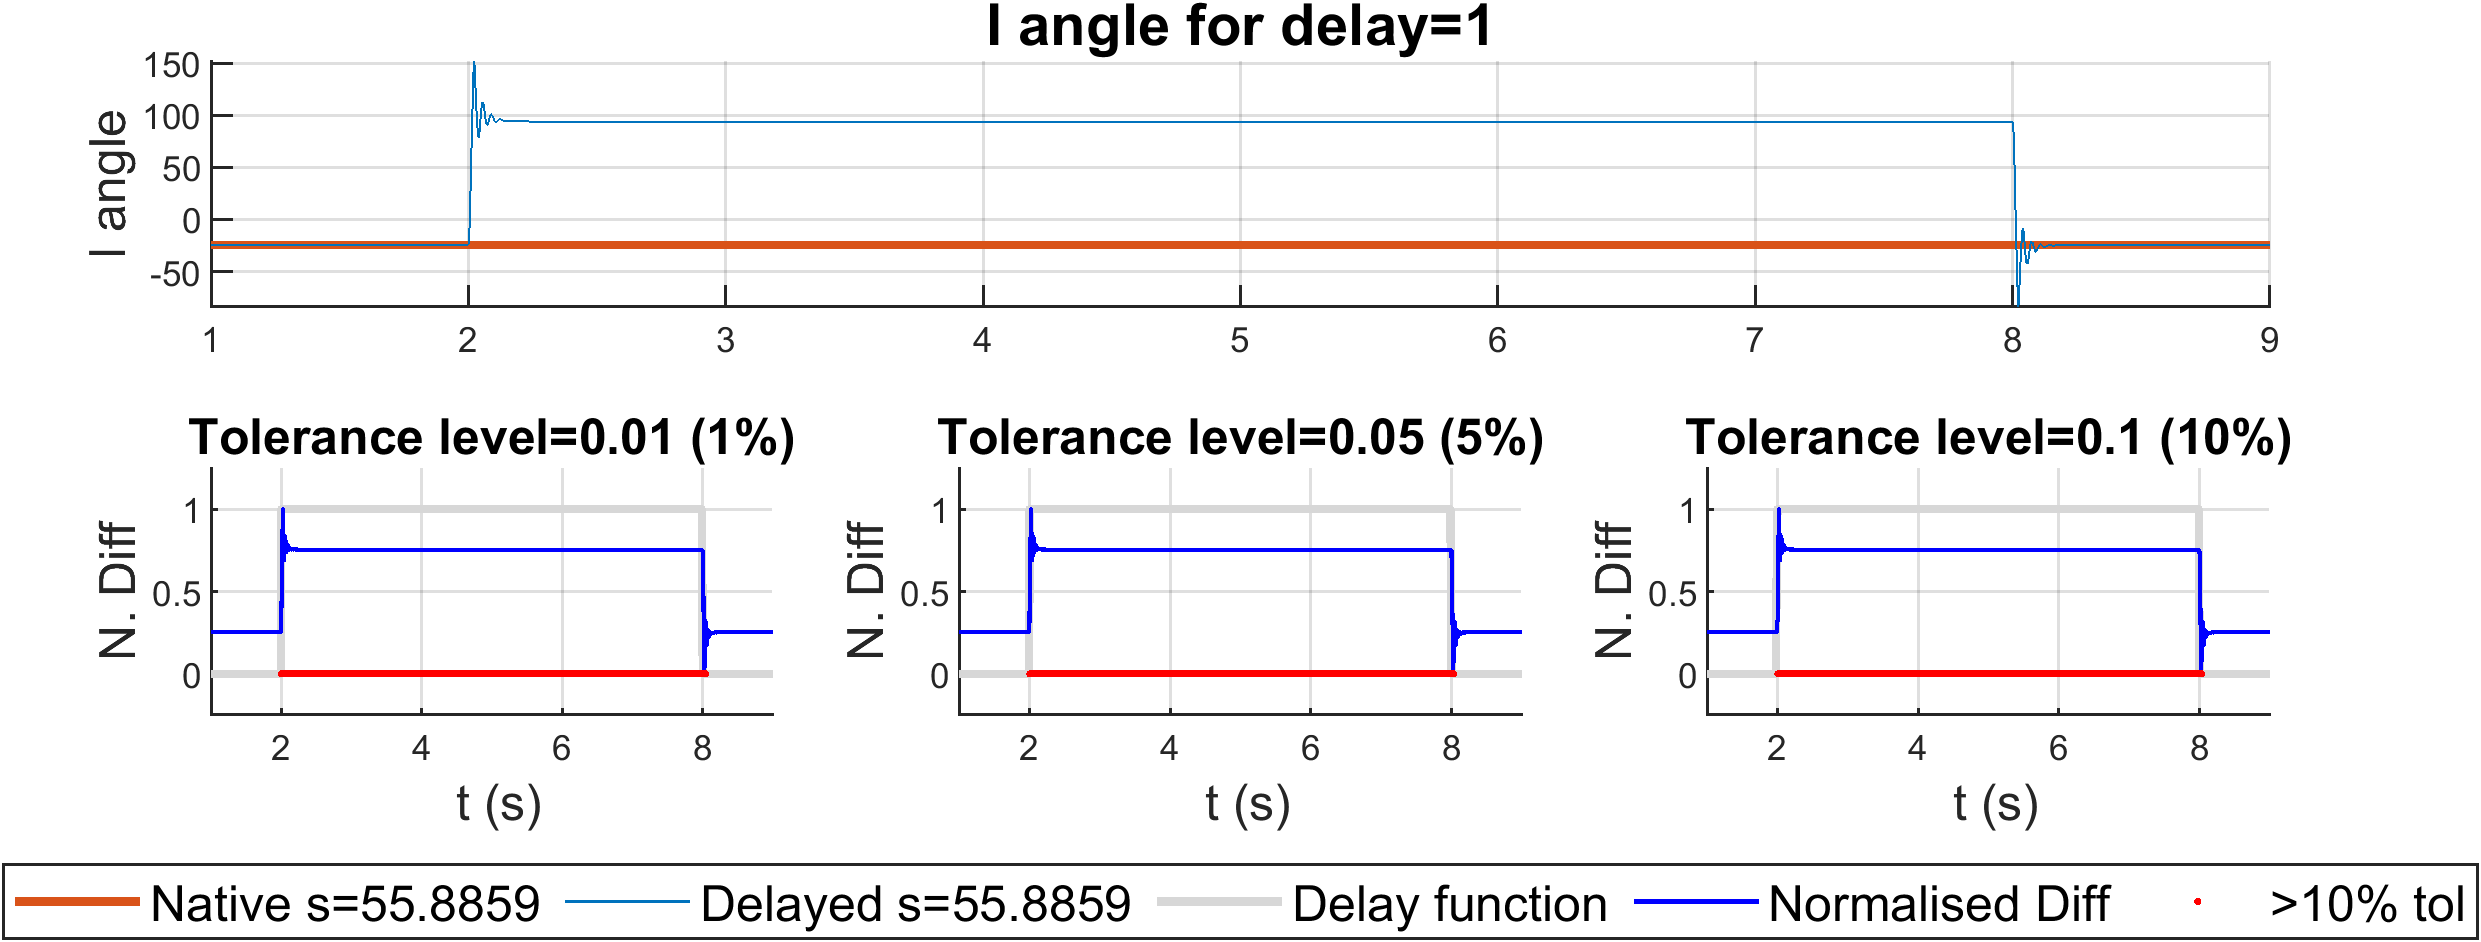
\includegraphics[width=0.95\textwidth]{PMUsim-figures/DelayOf_1/Instant_iAngle.png}}\\
   \label{fig:pmuOneAngle}
 %\caption{Instant Delay Angle Output for the Delay Level of One}
  \end{tabular}
\caption[Instant delay of 1: Angle Output]{Results for Angle Output for Delay equal to One}
 \end{figure}
 
\newpage 
\subsection{Instant Delay Level of Two}

\begin{small}
     \tcbox[size=normal, standard jigsaw, opacityback=0, boxrule=0pt,halign=justify]{
     Instant Delay Level of Two}{
          \begin{itemize}
         \item      The delayed signal (blue) overlaps the original signal (red), producing a straight line, colored neither red nor blue.
         \item  The blue Normalised diff signal also overlaps the grey delay function.
          \end{itemize} }
\end{small}


\newpage 
\begin{figure}[H]
\begin{tabular}{c}
   \fbox{     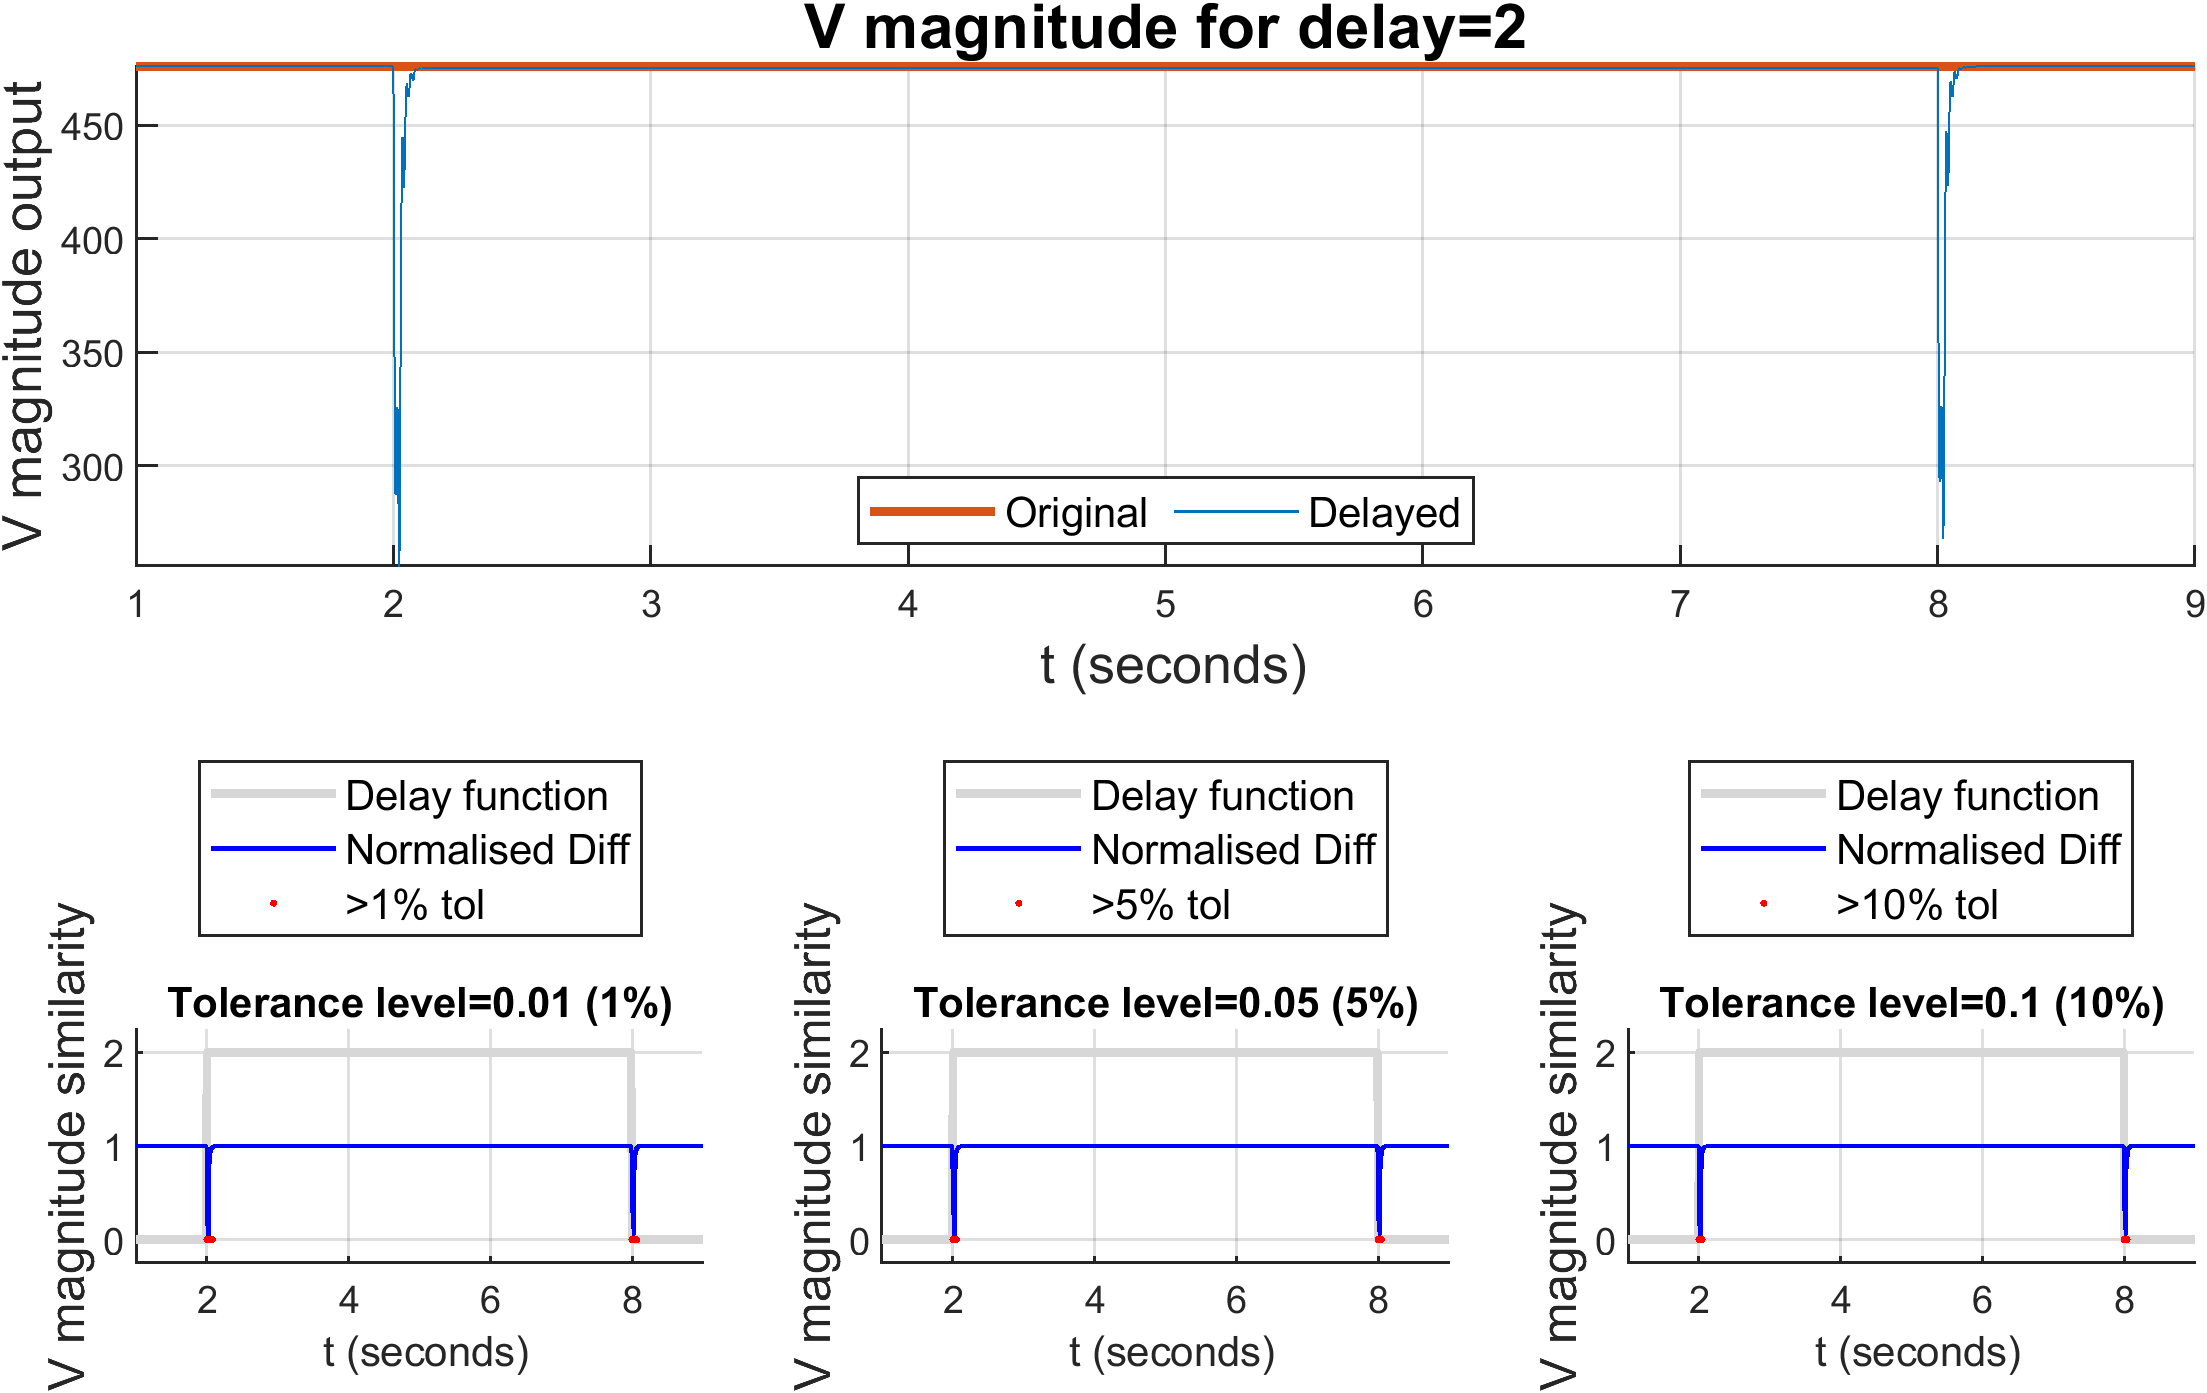
\includegraphics[width=0.95\textwidth]{PMUsim-figures/DelayOf_2/Instant_vMagnitude.png}}\\
    \\ 
    
   \fbox{   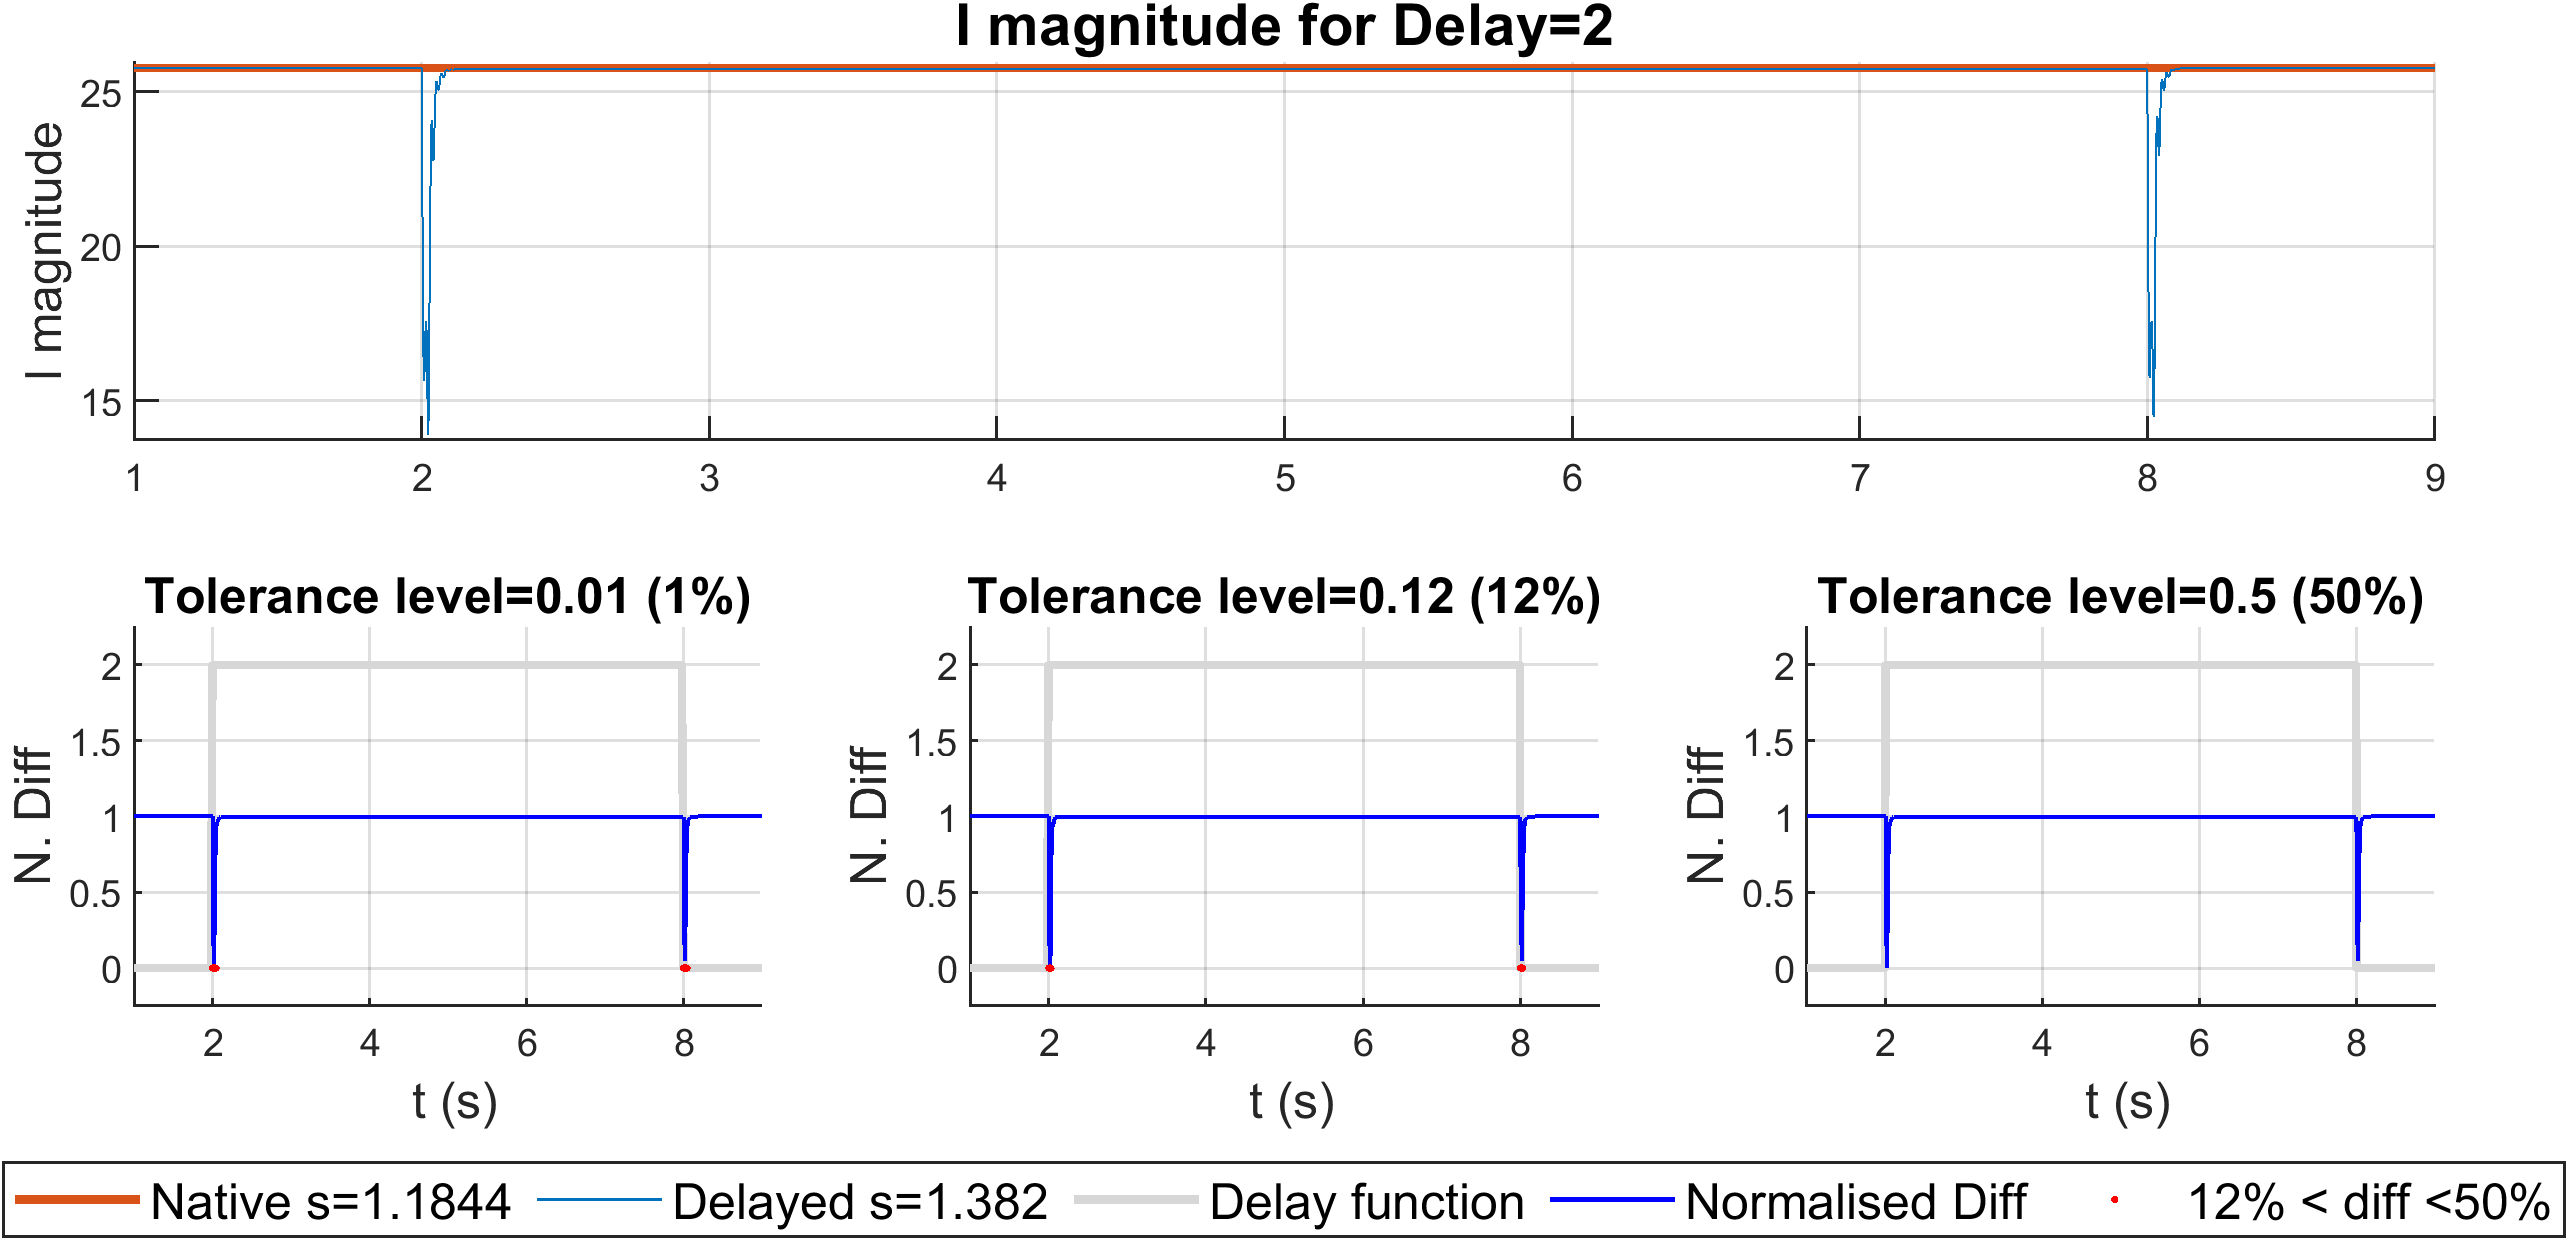
\includegraphics[width=0.95\textwidth]{PMUsim-figures/DelayOf_2/Instant_iMagnitude.png}}\\
 \label{fig:PMUsim_Two_Mag}
 %\caption{Instant Delay Magnitude Output for the Delay Level of Two}
  \end{tabular}
\caption[Instant delay of 2: Magnitude Output]{Results for Magnitude Output for Instant Delay equal to Two}
 \end{figure}

\newpage 
\begin{figure}[H]
\begin{tabular}{c}
   \fbox{     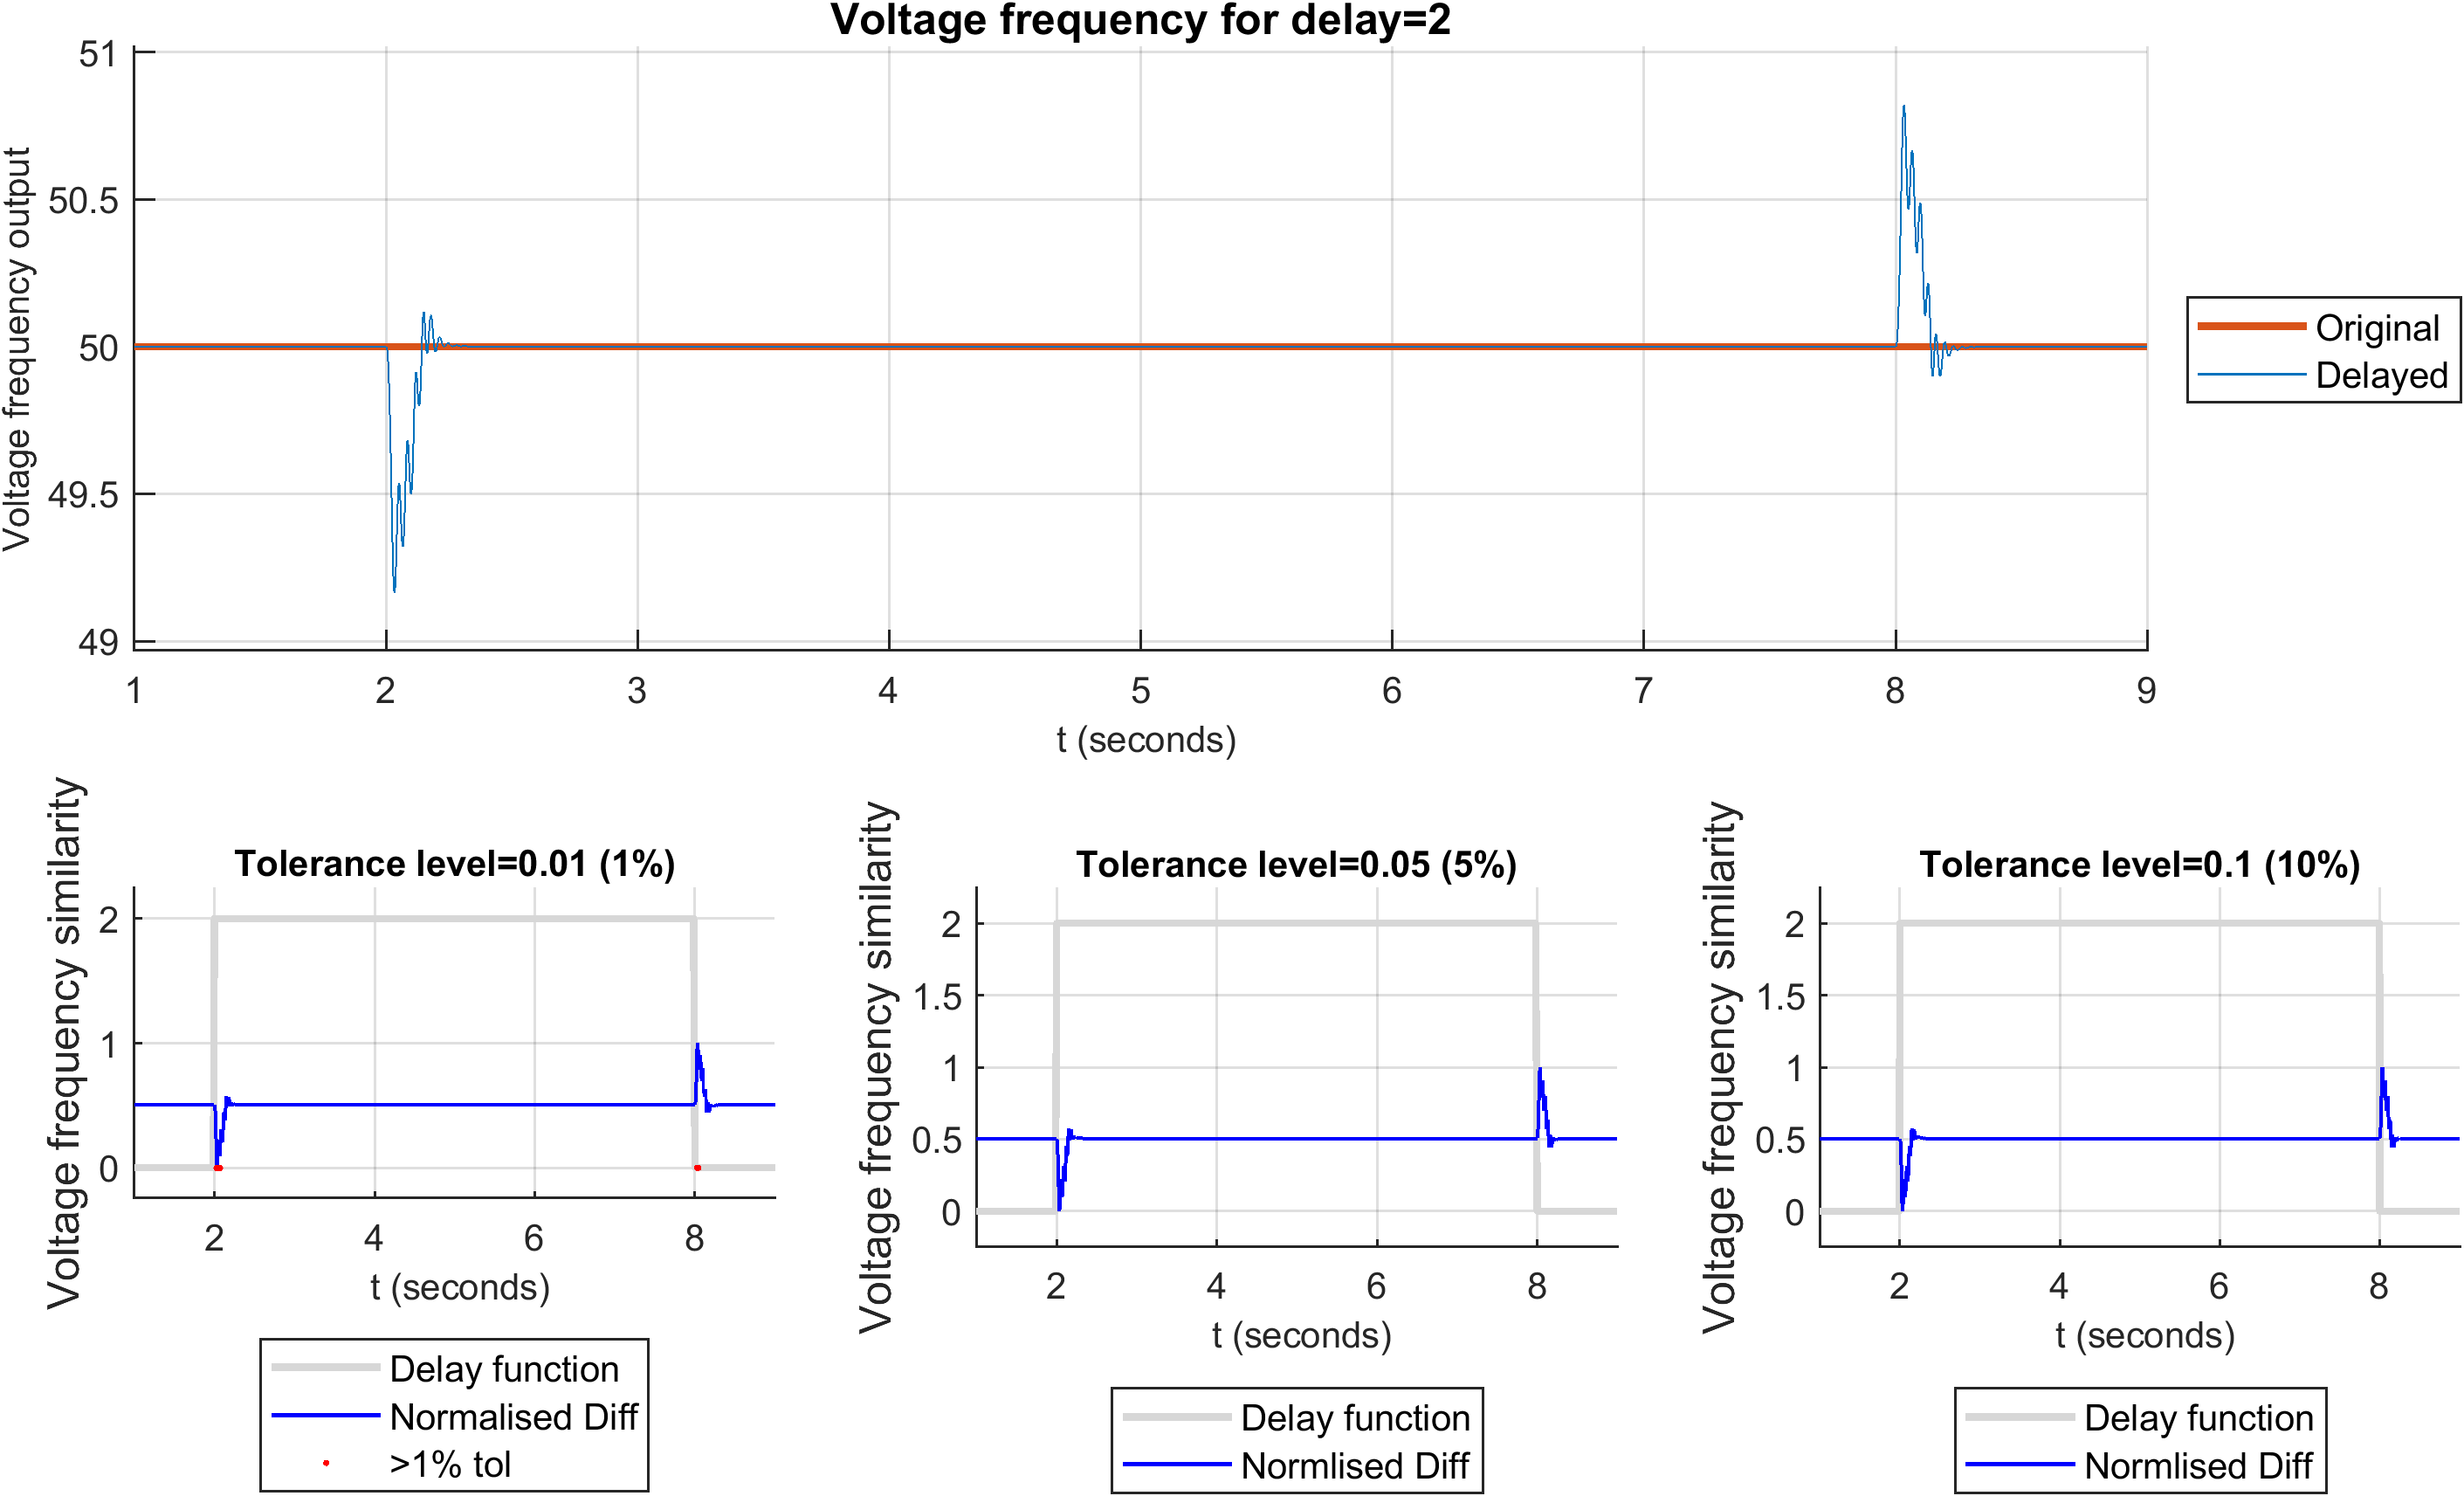
\includegraphics[width=0.95\textwidth]{PMUsim-figures/DelayOf_2/Instant_vFrequency.png}}\\
    \\ 
    
   \fbox{   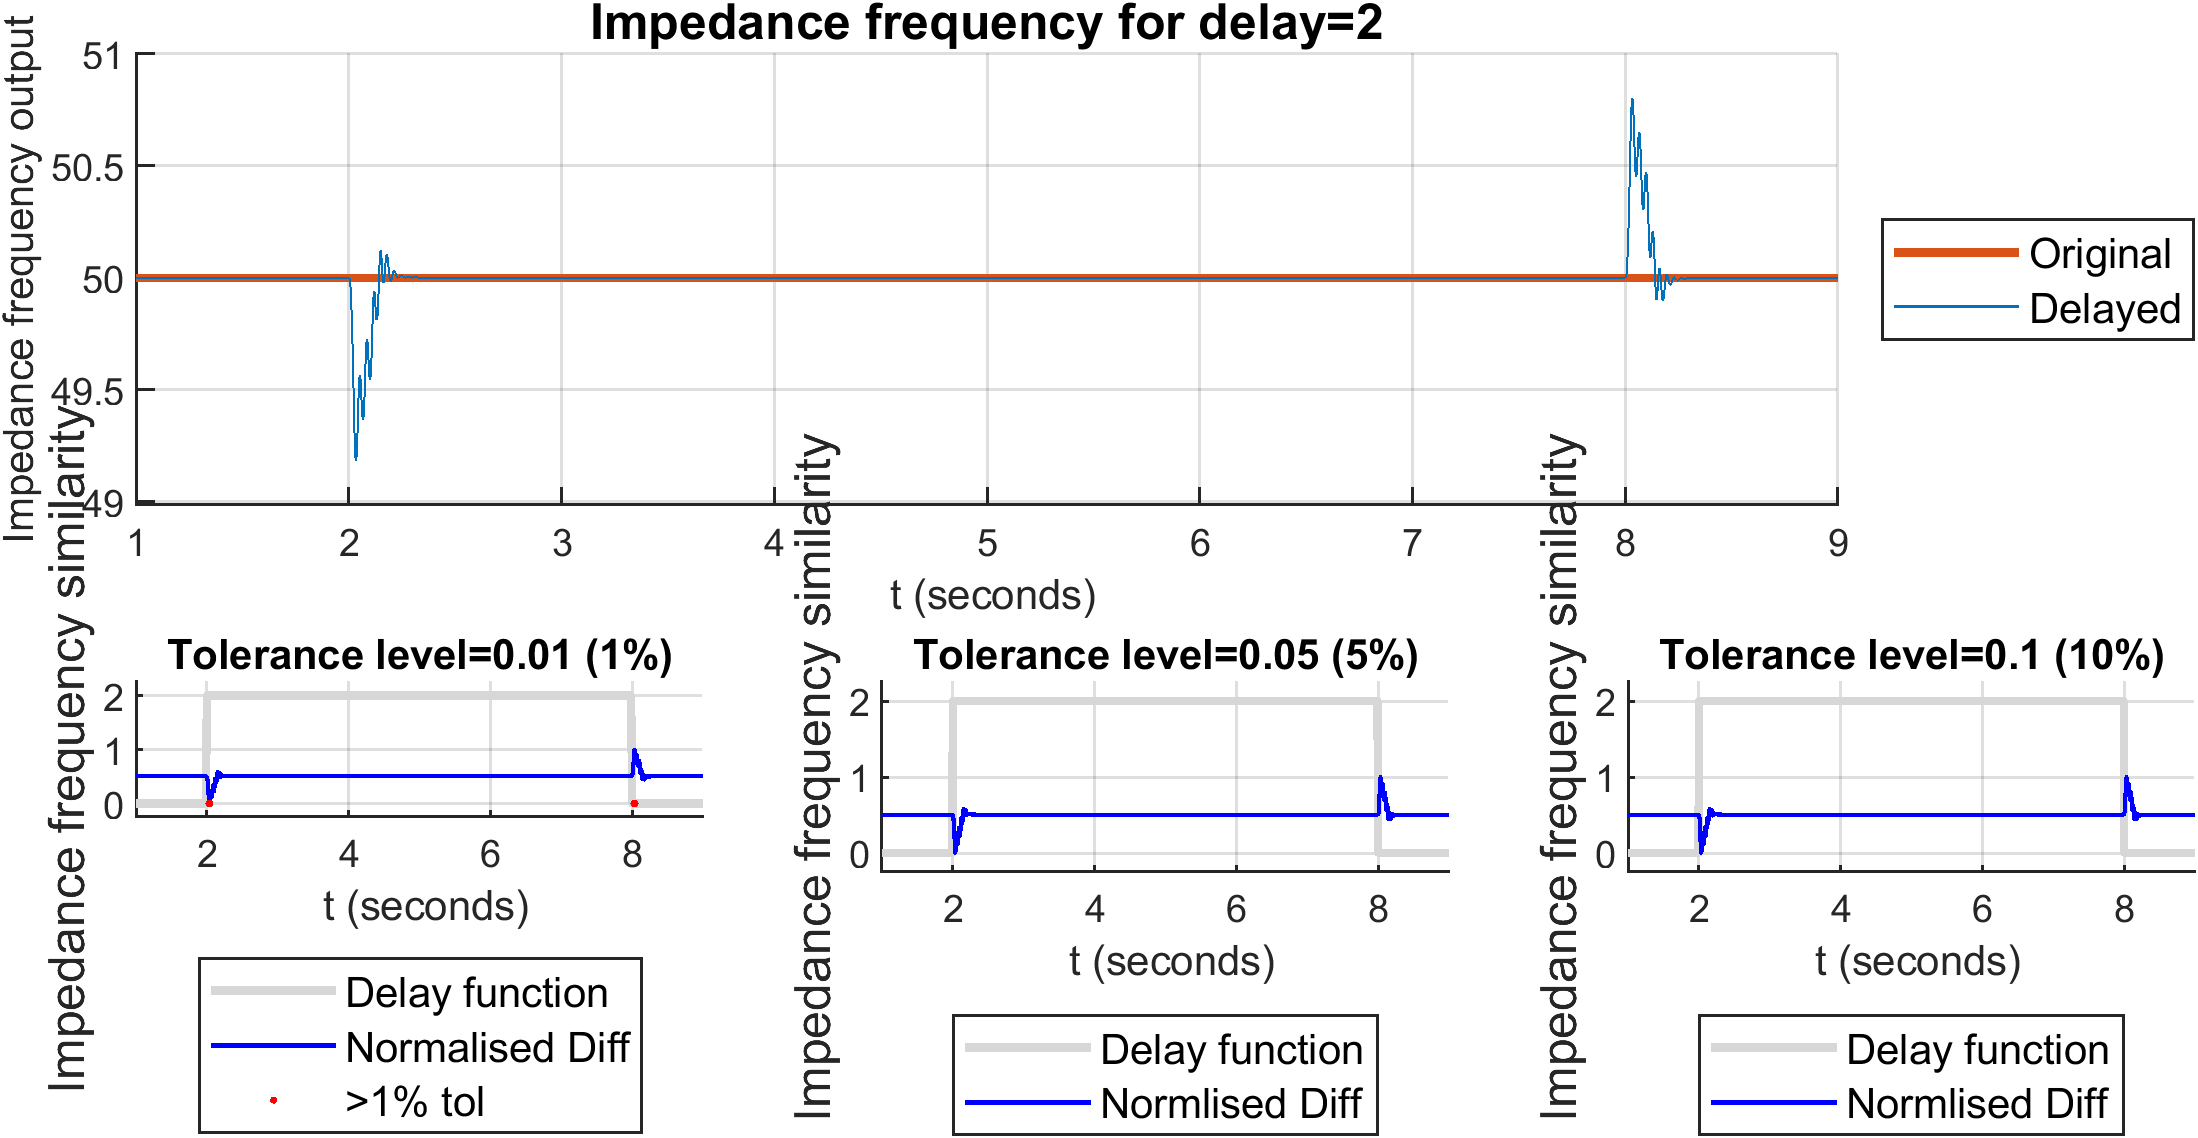
\includegraphics[width=0.95\textwidth]{PMUsim-figures/DelayOf_2/Instant_iFrequency.png}}\\   
 \label{fig:PMUsim_Two_Freq}
 %\caption{Instant Delay Frequency Output for the Delay Level of Two}
  \end{tabular}
\caption[Instant delay of 2: Frequency Output]{Results for Frequency Output for Instant Delay equal to Two}
 \end{figure}


\newpage 
\begin{figure}[H]
\begin{tabular}{c}
   \fbox{     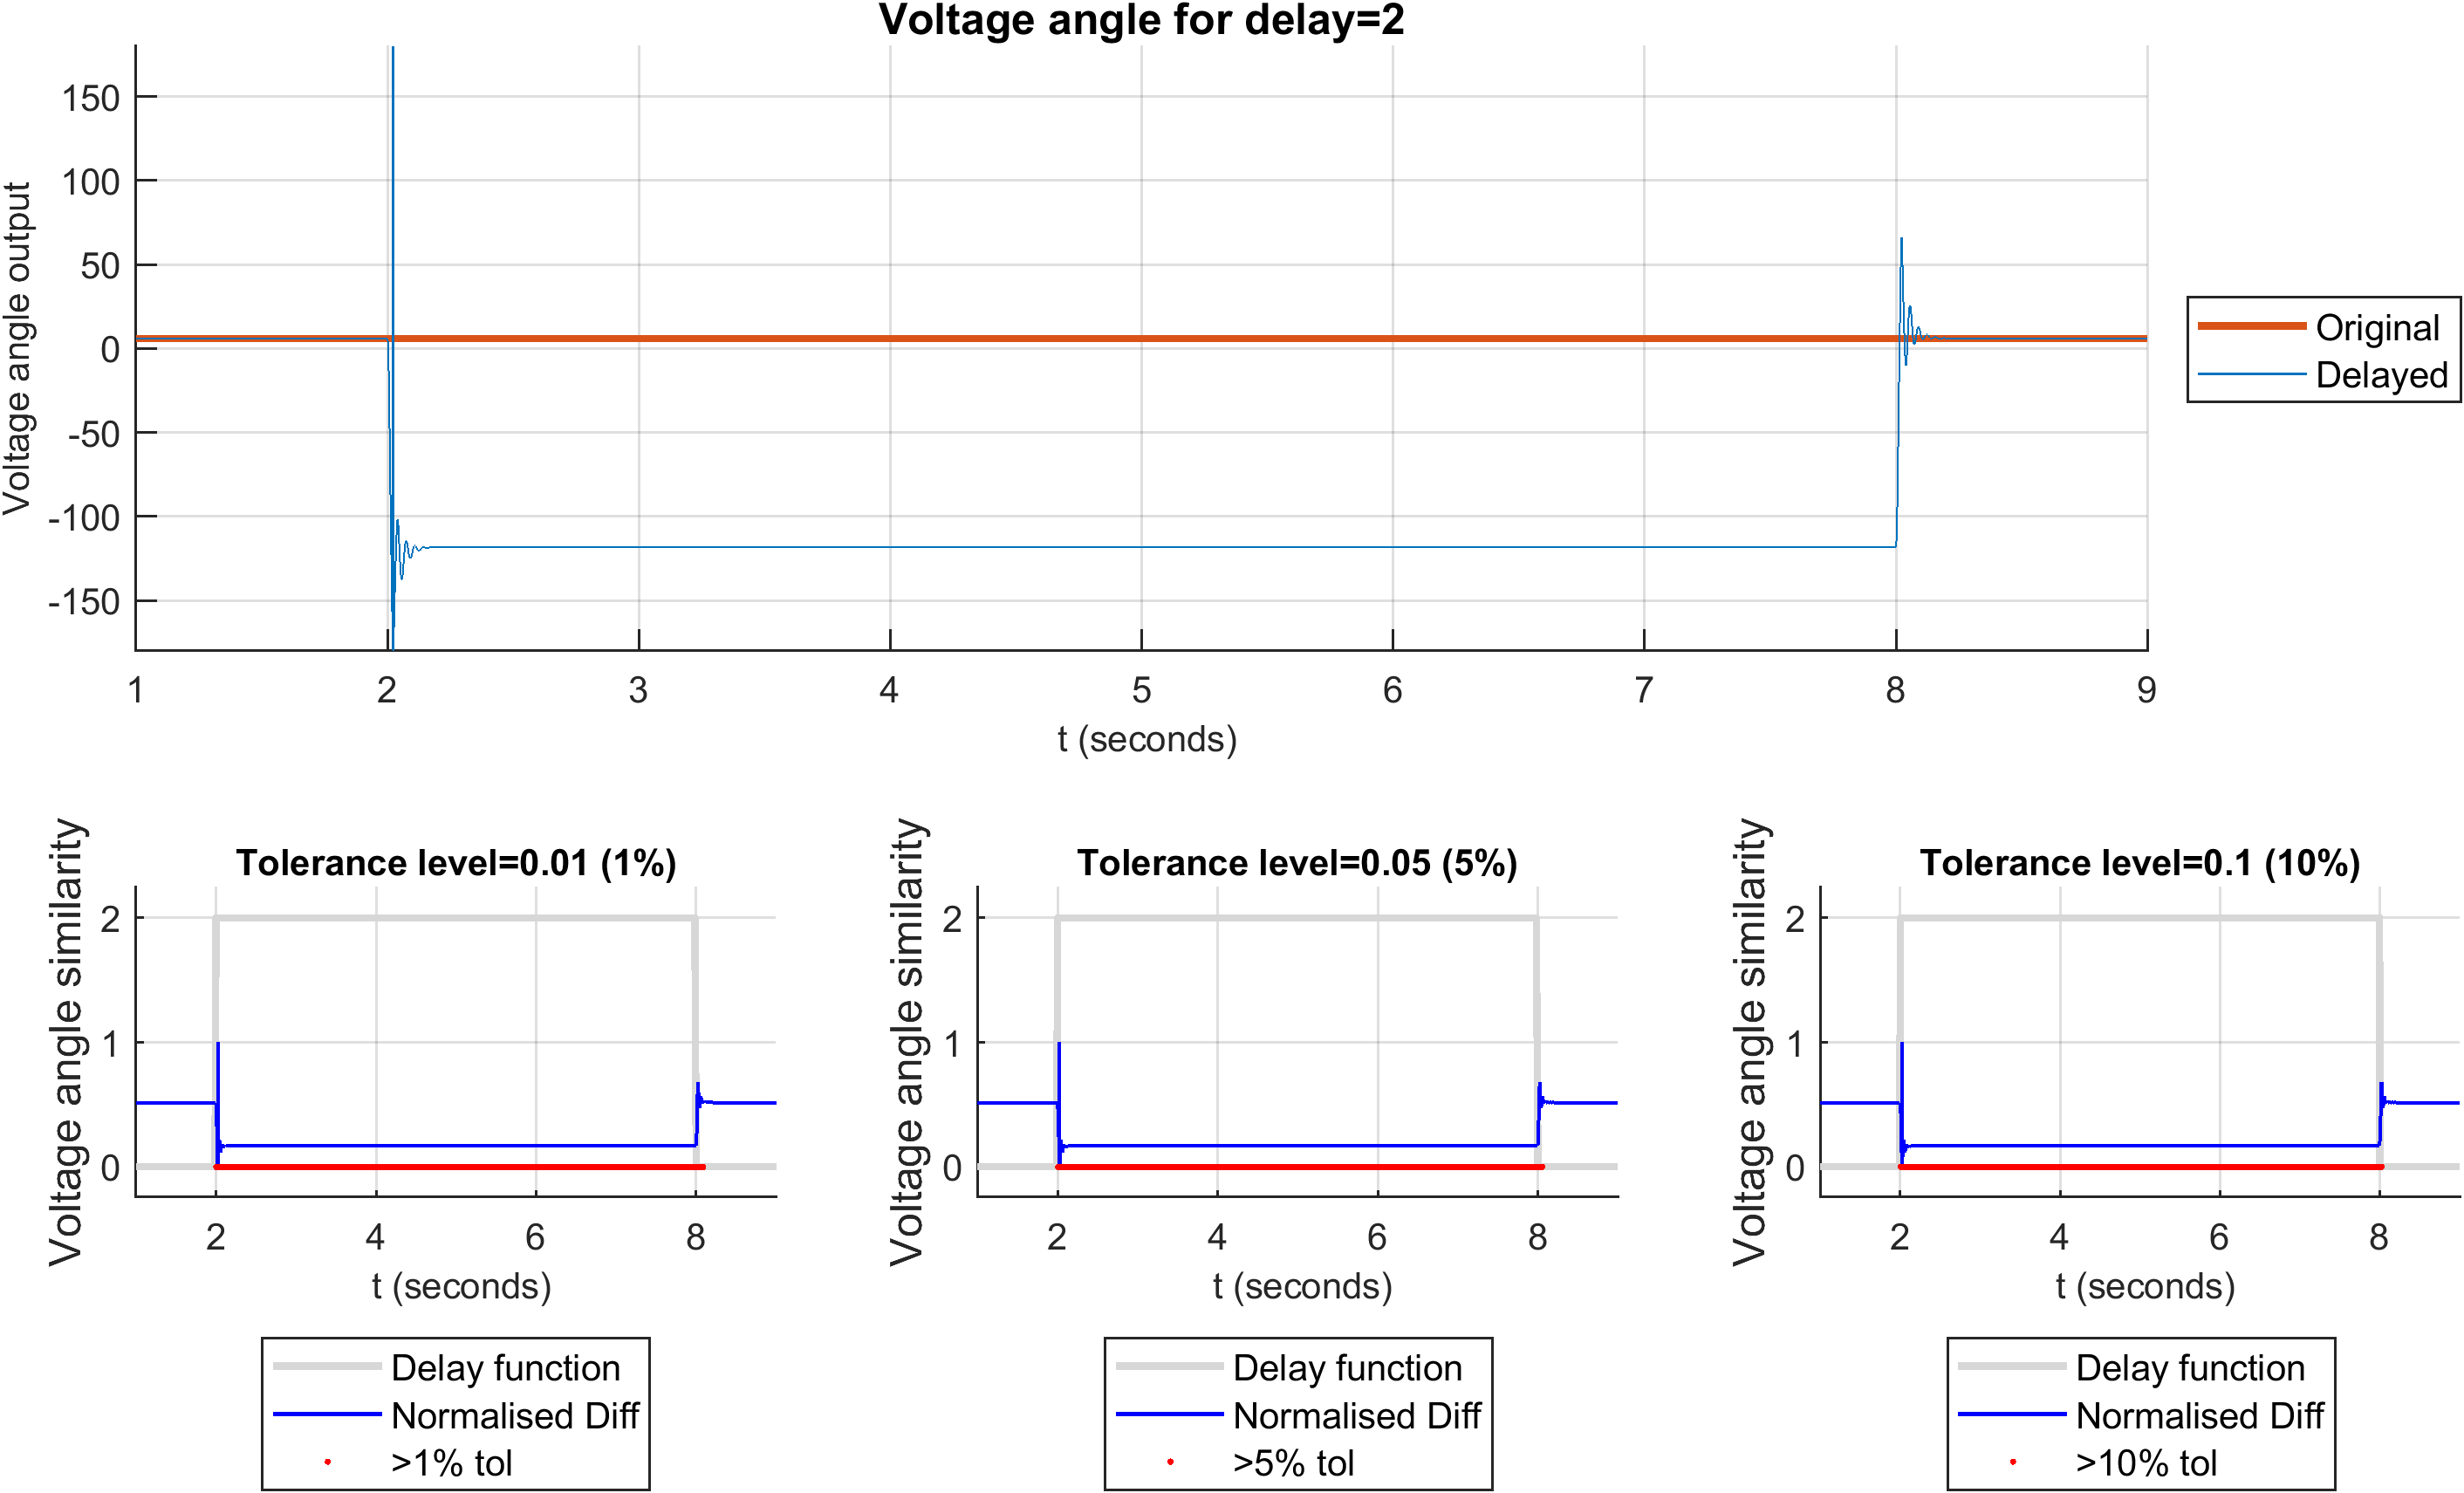
\includegraphics[width=0.95\textwidth]{PMUsim-figures/DelayOf_2/Instant_vAngle.png}}\\
  \\ 
   \fbox{   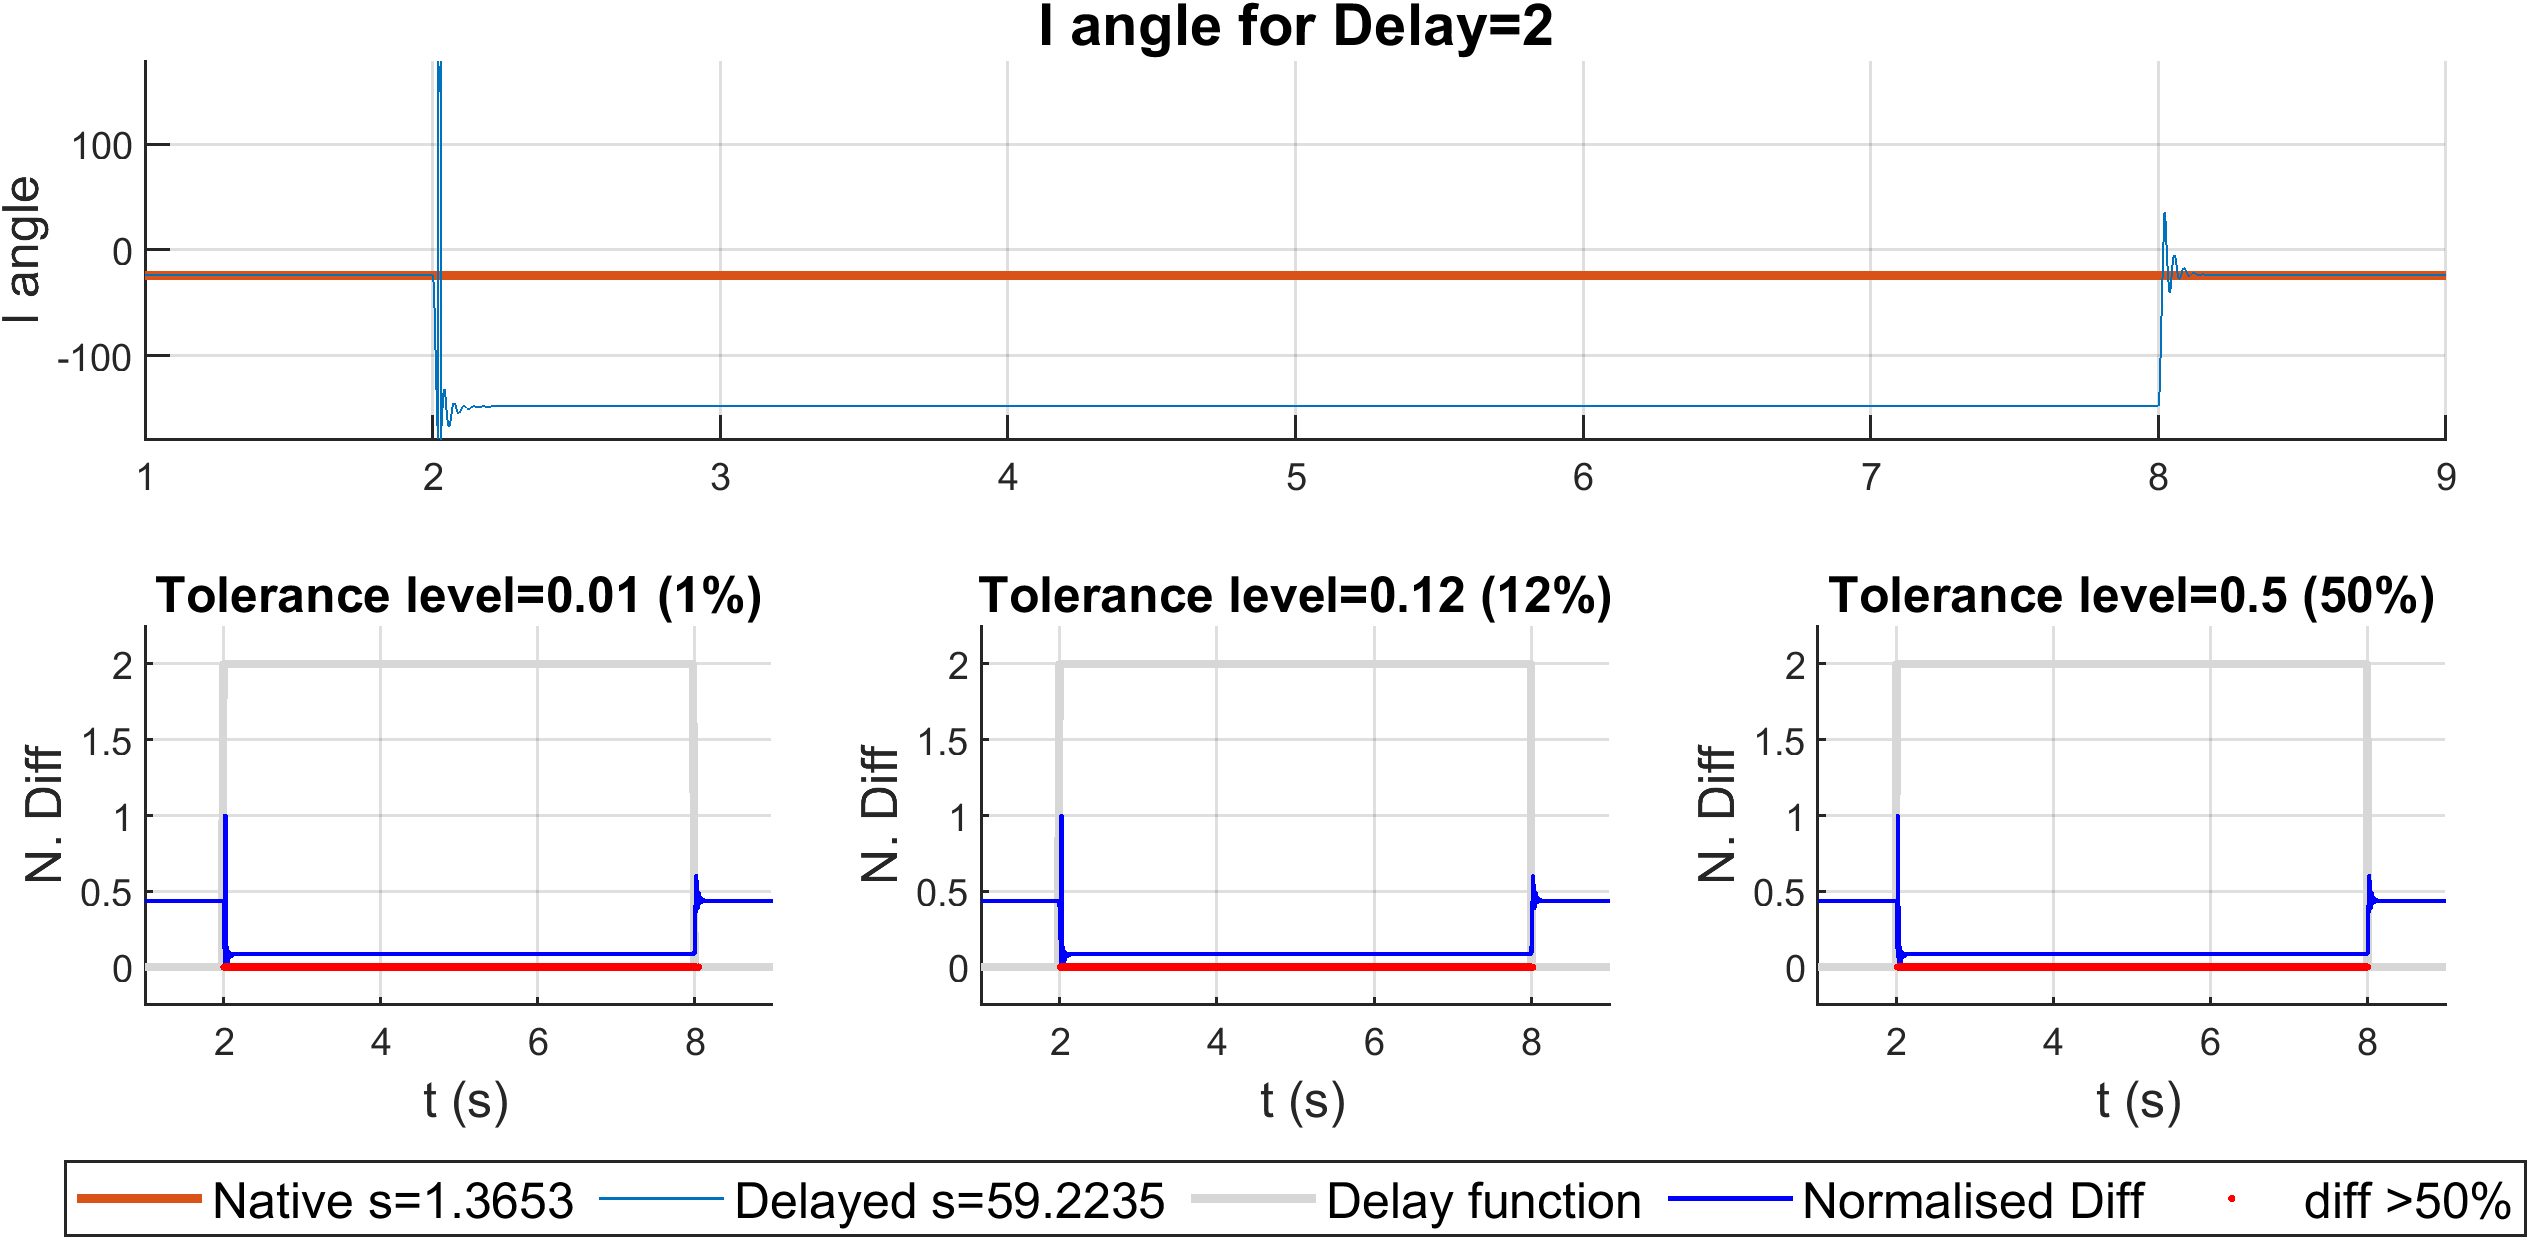
\includegraphics[width=0.95\textwidth]{PMUsim-figures/DelayOf_2/Instant_iAngle.png}}\\
 \label{fig:PMUsim_Two_Angle}
 %\caption{Instant Delay Angle Output for the Delay Level of Two}
  \end{tabular}
\caption[Instant delay of 2: Angle Output]{Results for Angle Output for Instant Delay equal to Two}
 \end{figure}


\newpage 
\subsection{Instant Delay Level of Three}

\begin{small}
     \tcbox[size=normal, standard jigsaw, opacityback=0, boxrule=0pt,halign=justify]{
     Instant Delay Level of Three}{
          \begin{itemize}
         \item      The delayed signal (blue) overlaps the original signal (red), producing a straight line, colored neither red nor blue.
         \item  The blue Normalised diff signal also overlaps the grey delay function.
          \end{itemize} }
\end{small}



\newpage 
\begin{figure}[H]
\begin{tabular}{c}
   \fbox{    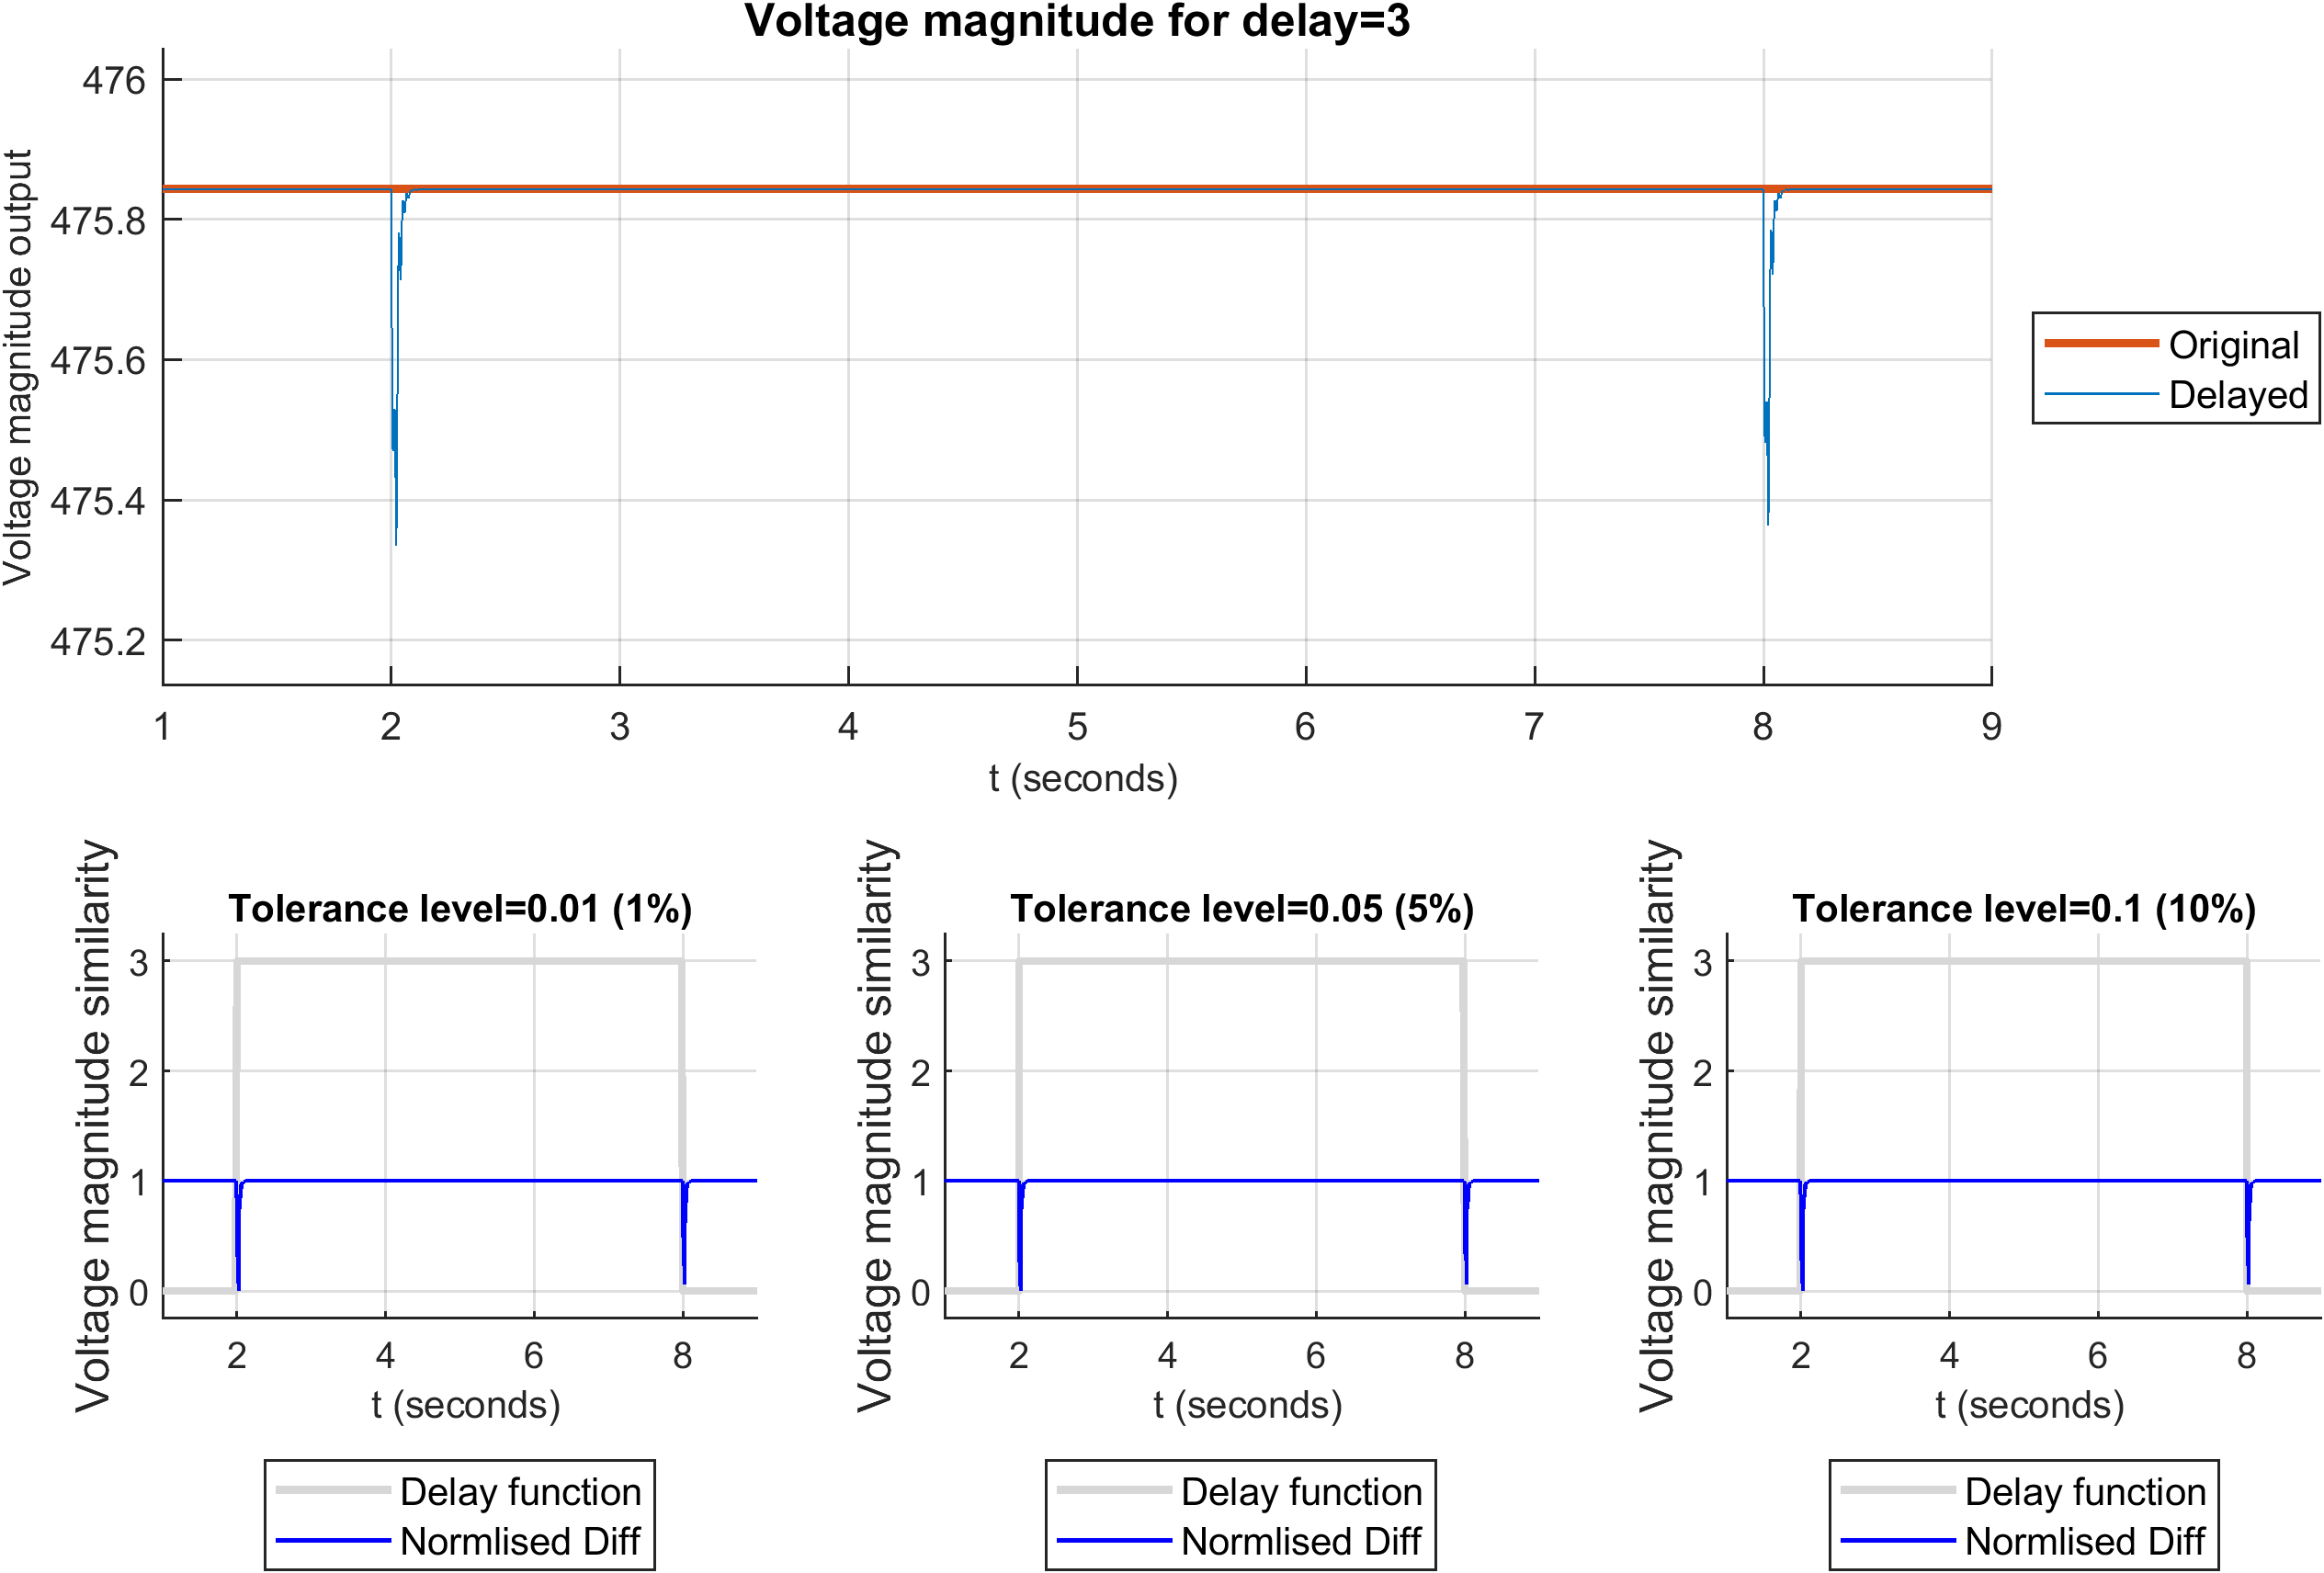
\includegraphics[width=0.95\textwidth]{PMUsim-figures/DelayOf_3/Instant_vMagnitude.png}}\\
    \\ 
    
   \fbox{  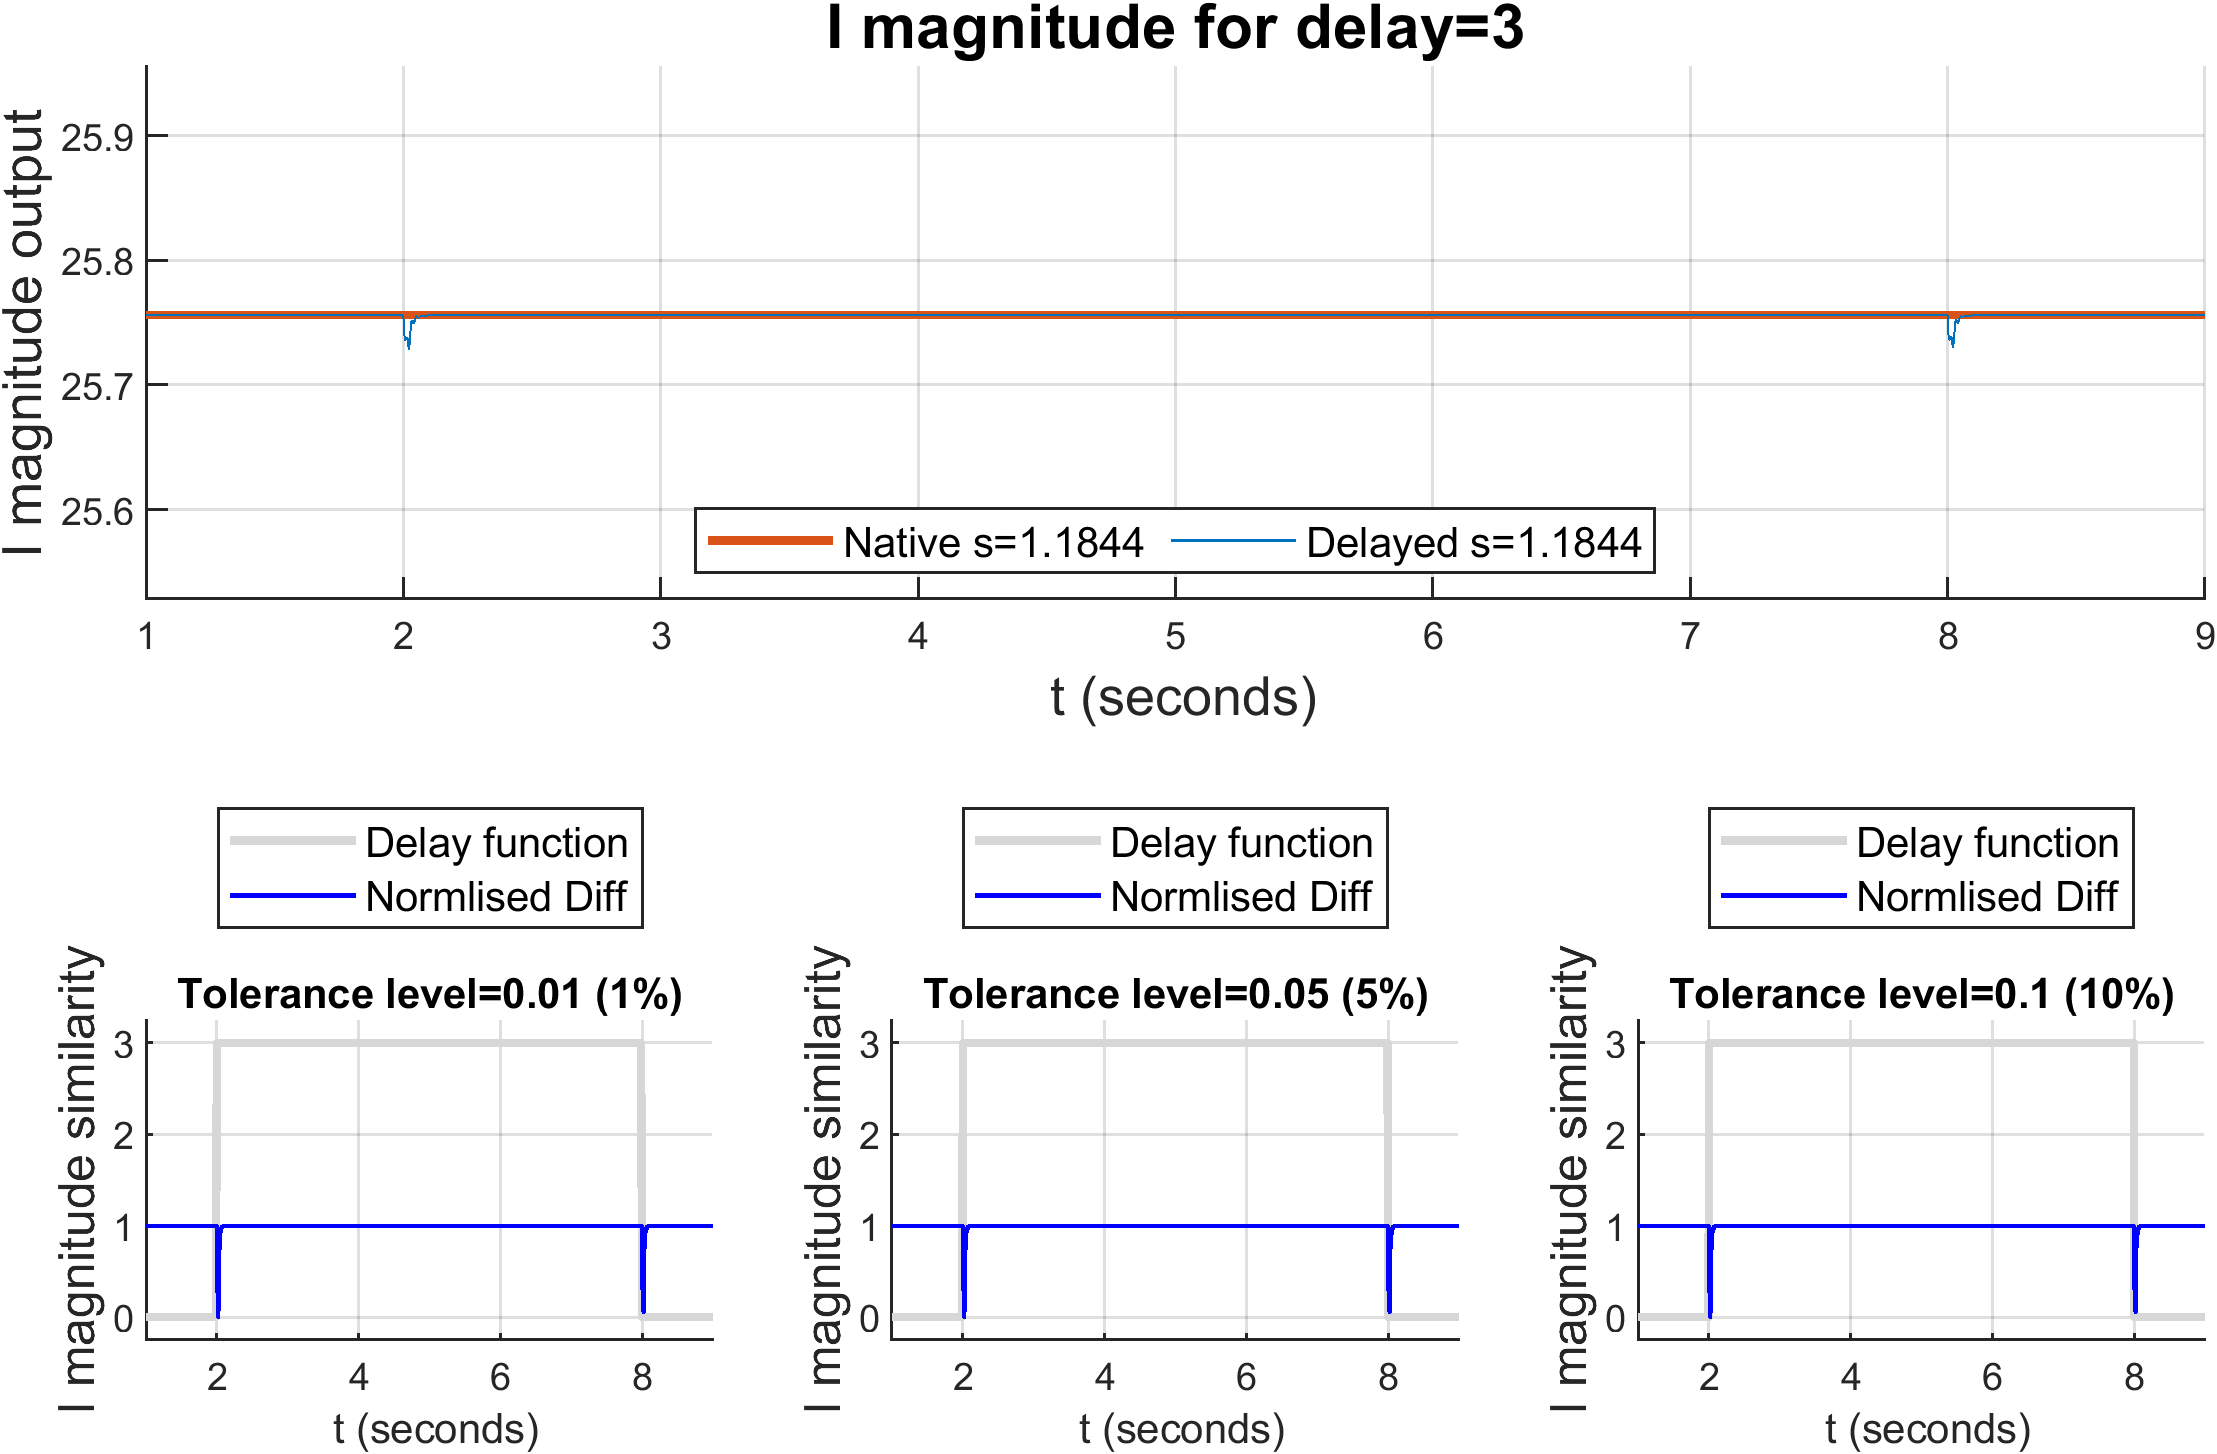
\includegraphics[width=0.95\textwidth]{PMUsim-figures/DelayOf_3/Instant_iMagnitude.png}}\\
 \label{fig:PMUsim_Three_Mag}
 %\caption{Instant Delay Magnitude Output for the Delay Level of Three}
  \end{tabular}
\caption[Instant delay of 3: Magnitude Output]{Results for Magnitude Output for Instant Delay equal to Three}
 \end{figure}

\newpage  
\begin{figure}[H]
\begin{tabular}{c}
   \fbox{    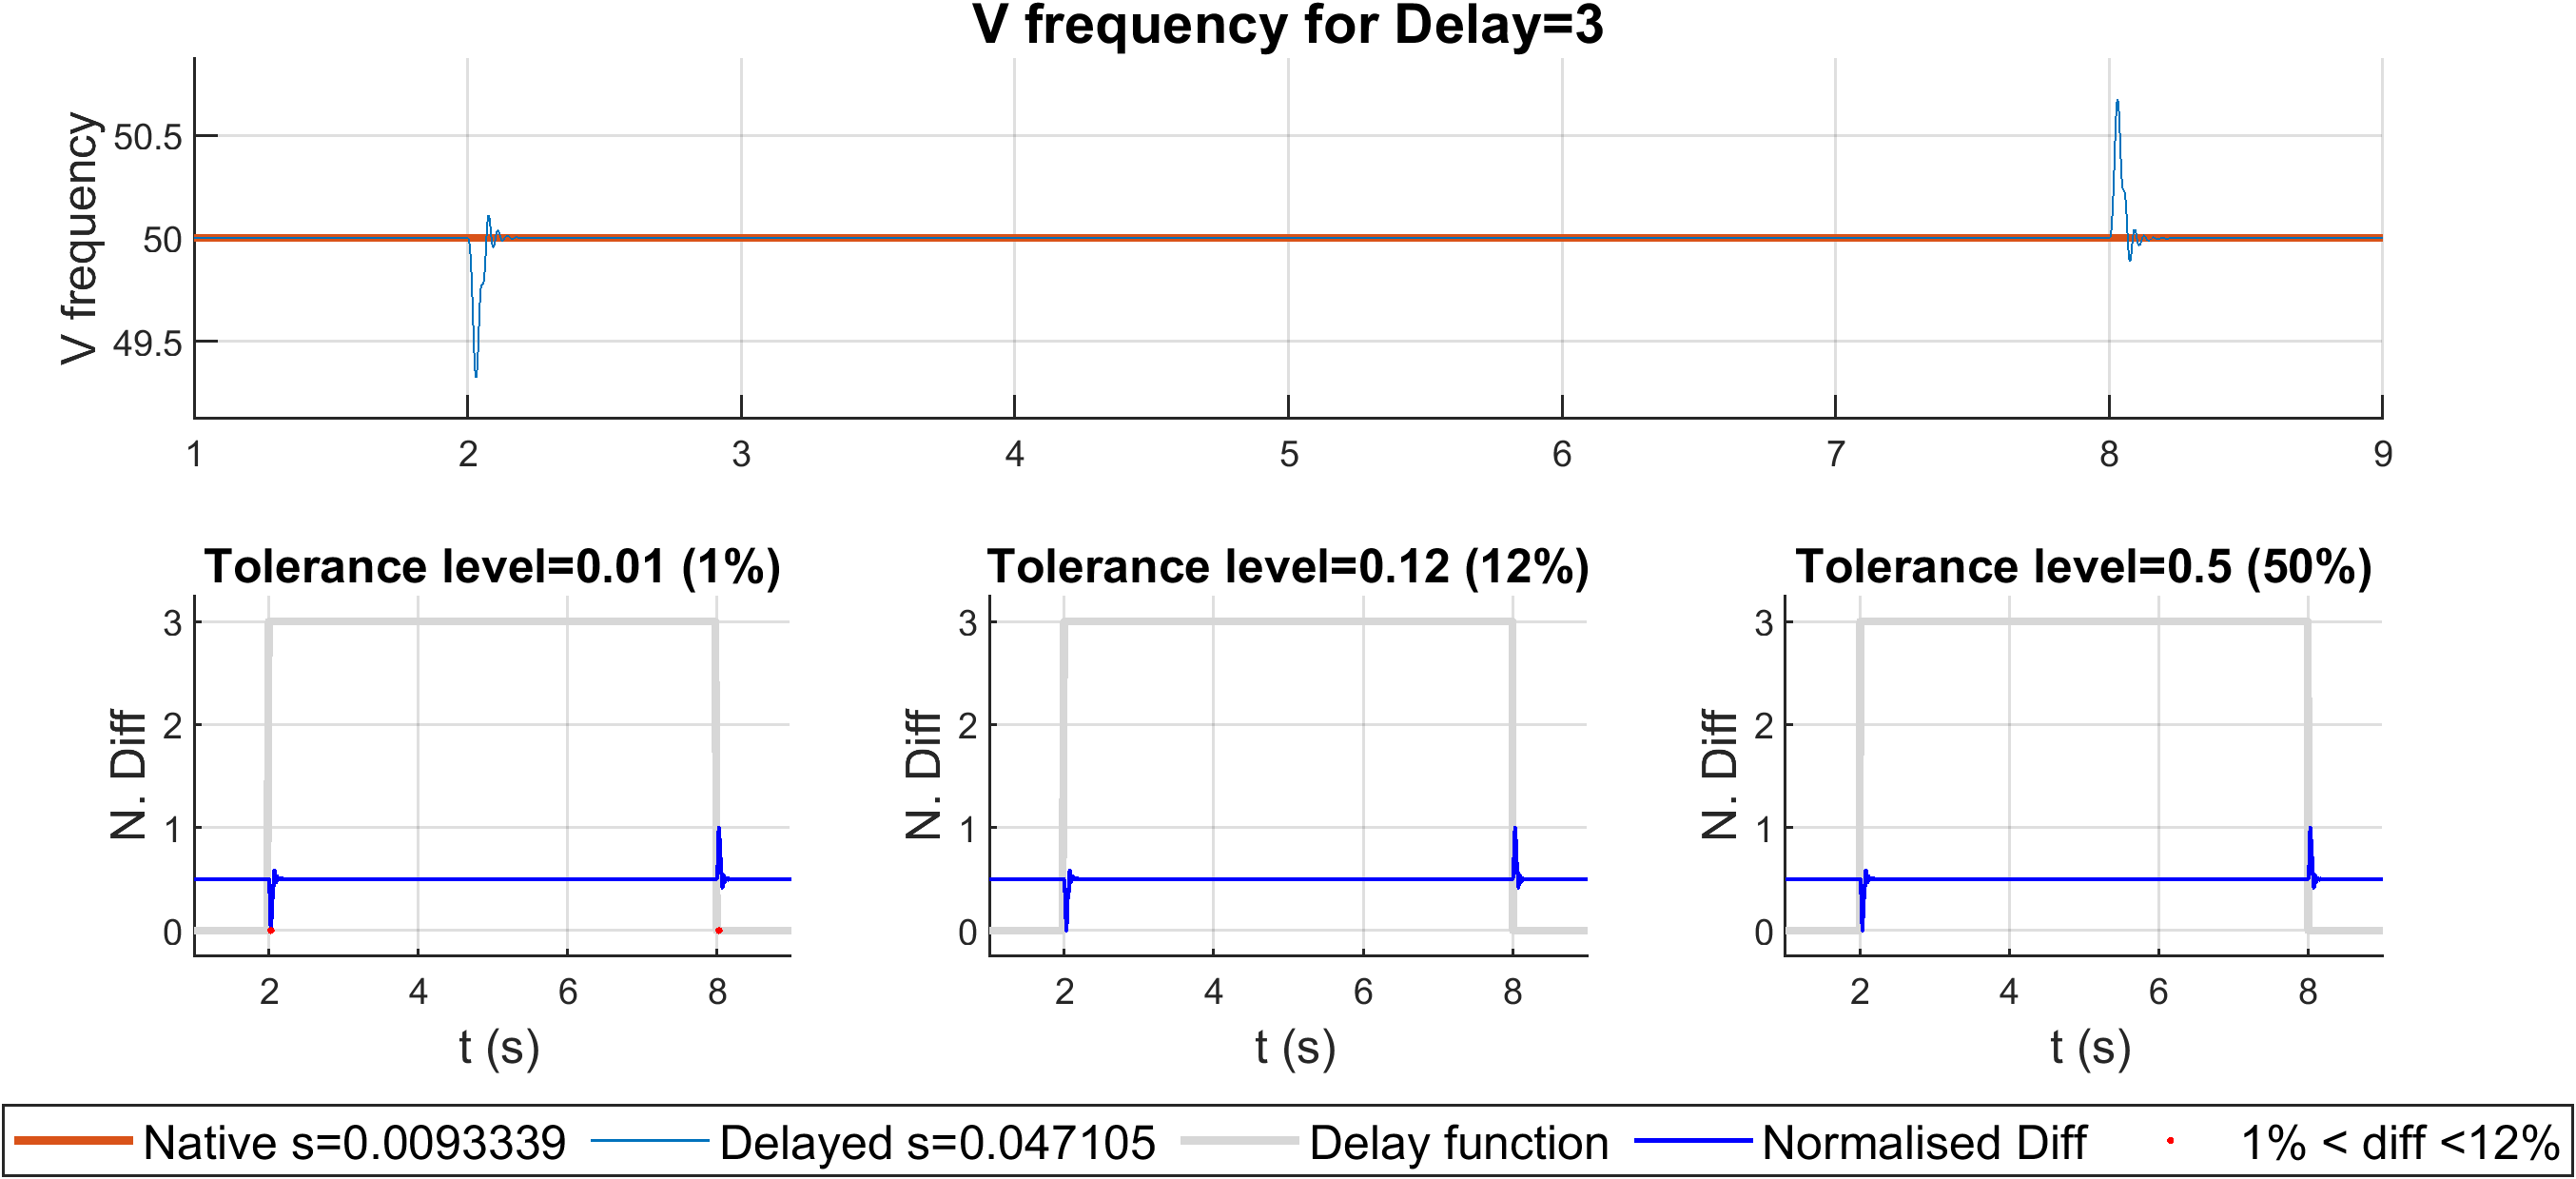
\includegraphics[width=0.95\textwidth]{PMUsim-figures/DelayOf_3/Instant_vFrequency.png}}\\
    \\ 
    
   \fbox{  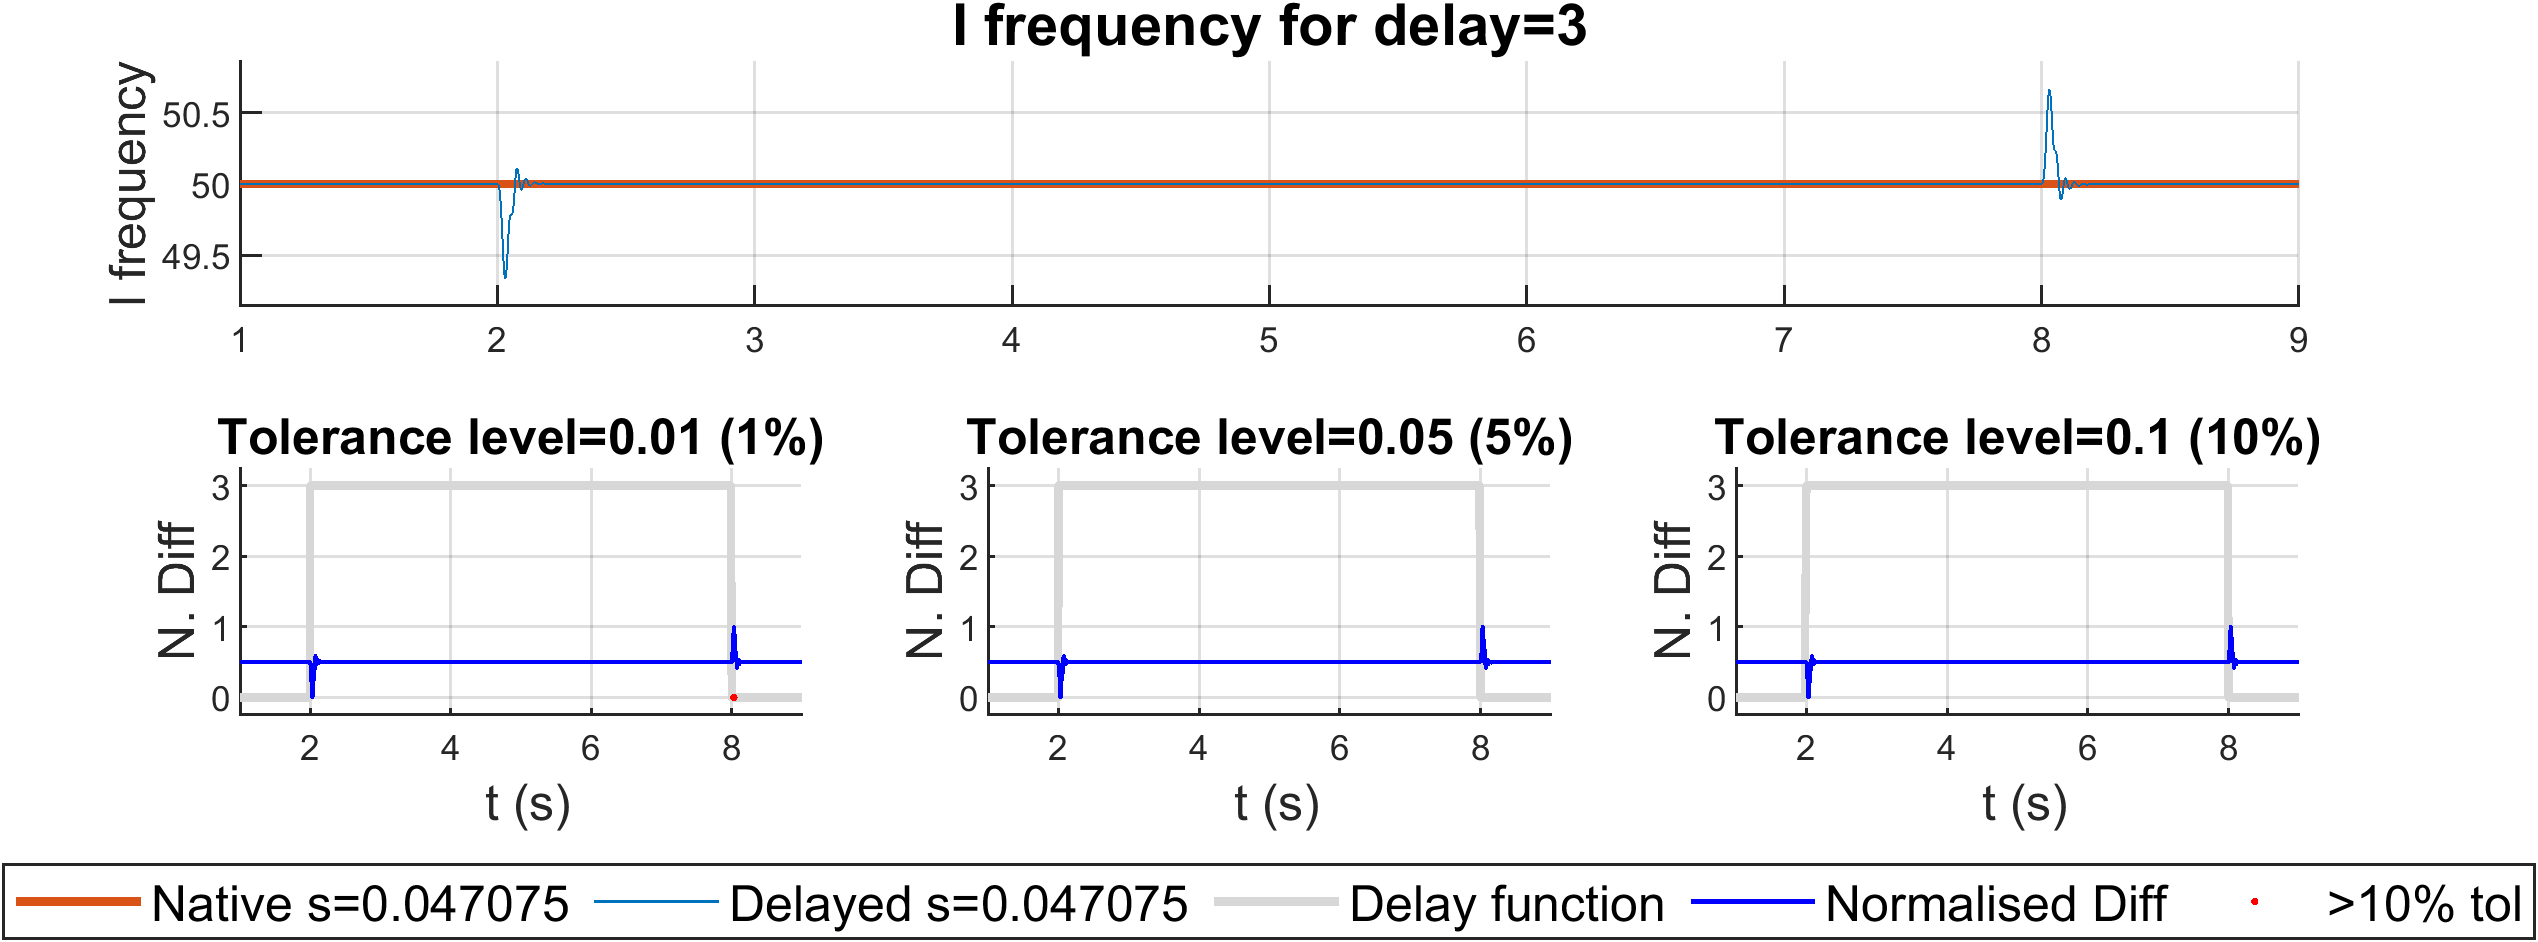
\includegraphics[width=0.95\textwidth]{PMUsim-figures/DelayOf_3/Instant_iFrequency.png}}\\
 \label{fig:PMUsim_Three_Freq}
 %\caption{Instant Delay Frequency Output for the Delay Level of Three}
  \end{tabular}
\caption[Instant delay of 3: Frequency Output]{Results for Frequency Output for Instant Delay equal to Three}
 \end{figure}


\newpage
\begin{figure}[H]
\begin{tabular}{c}
   \fbox{     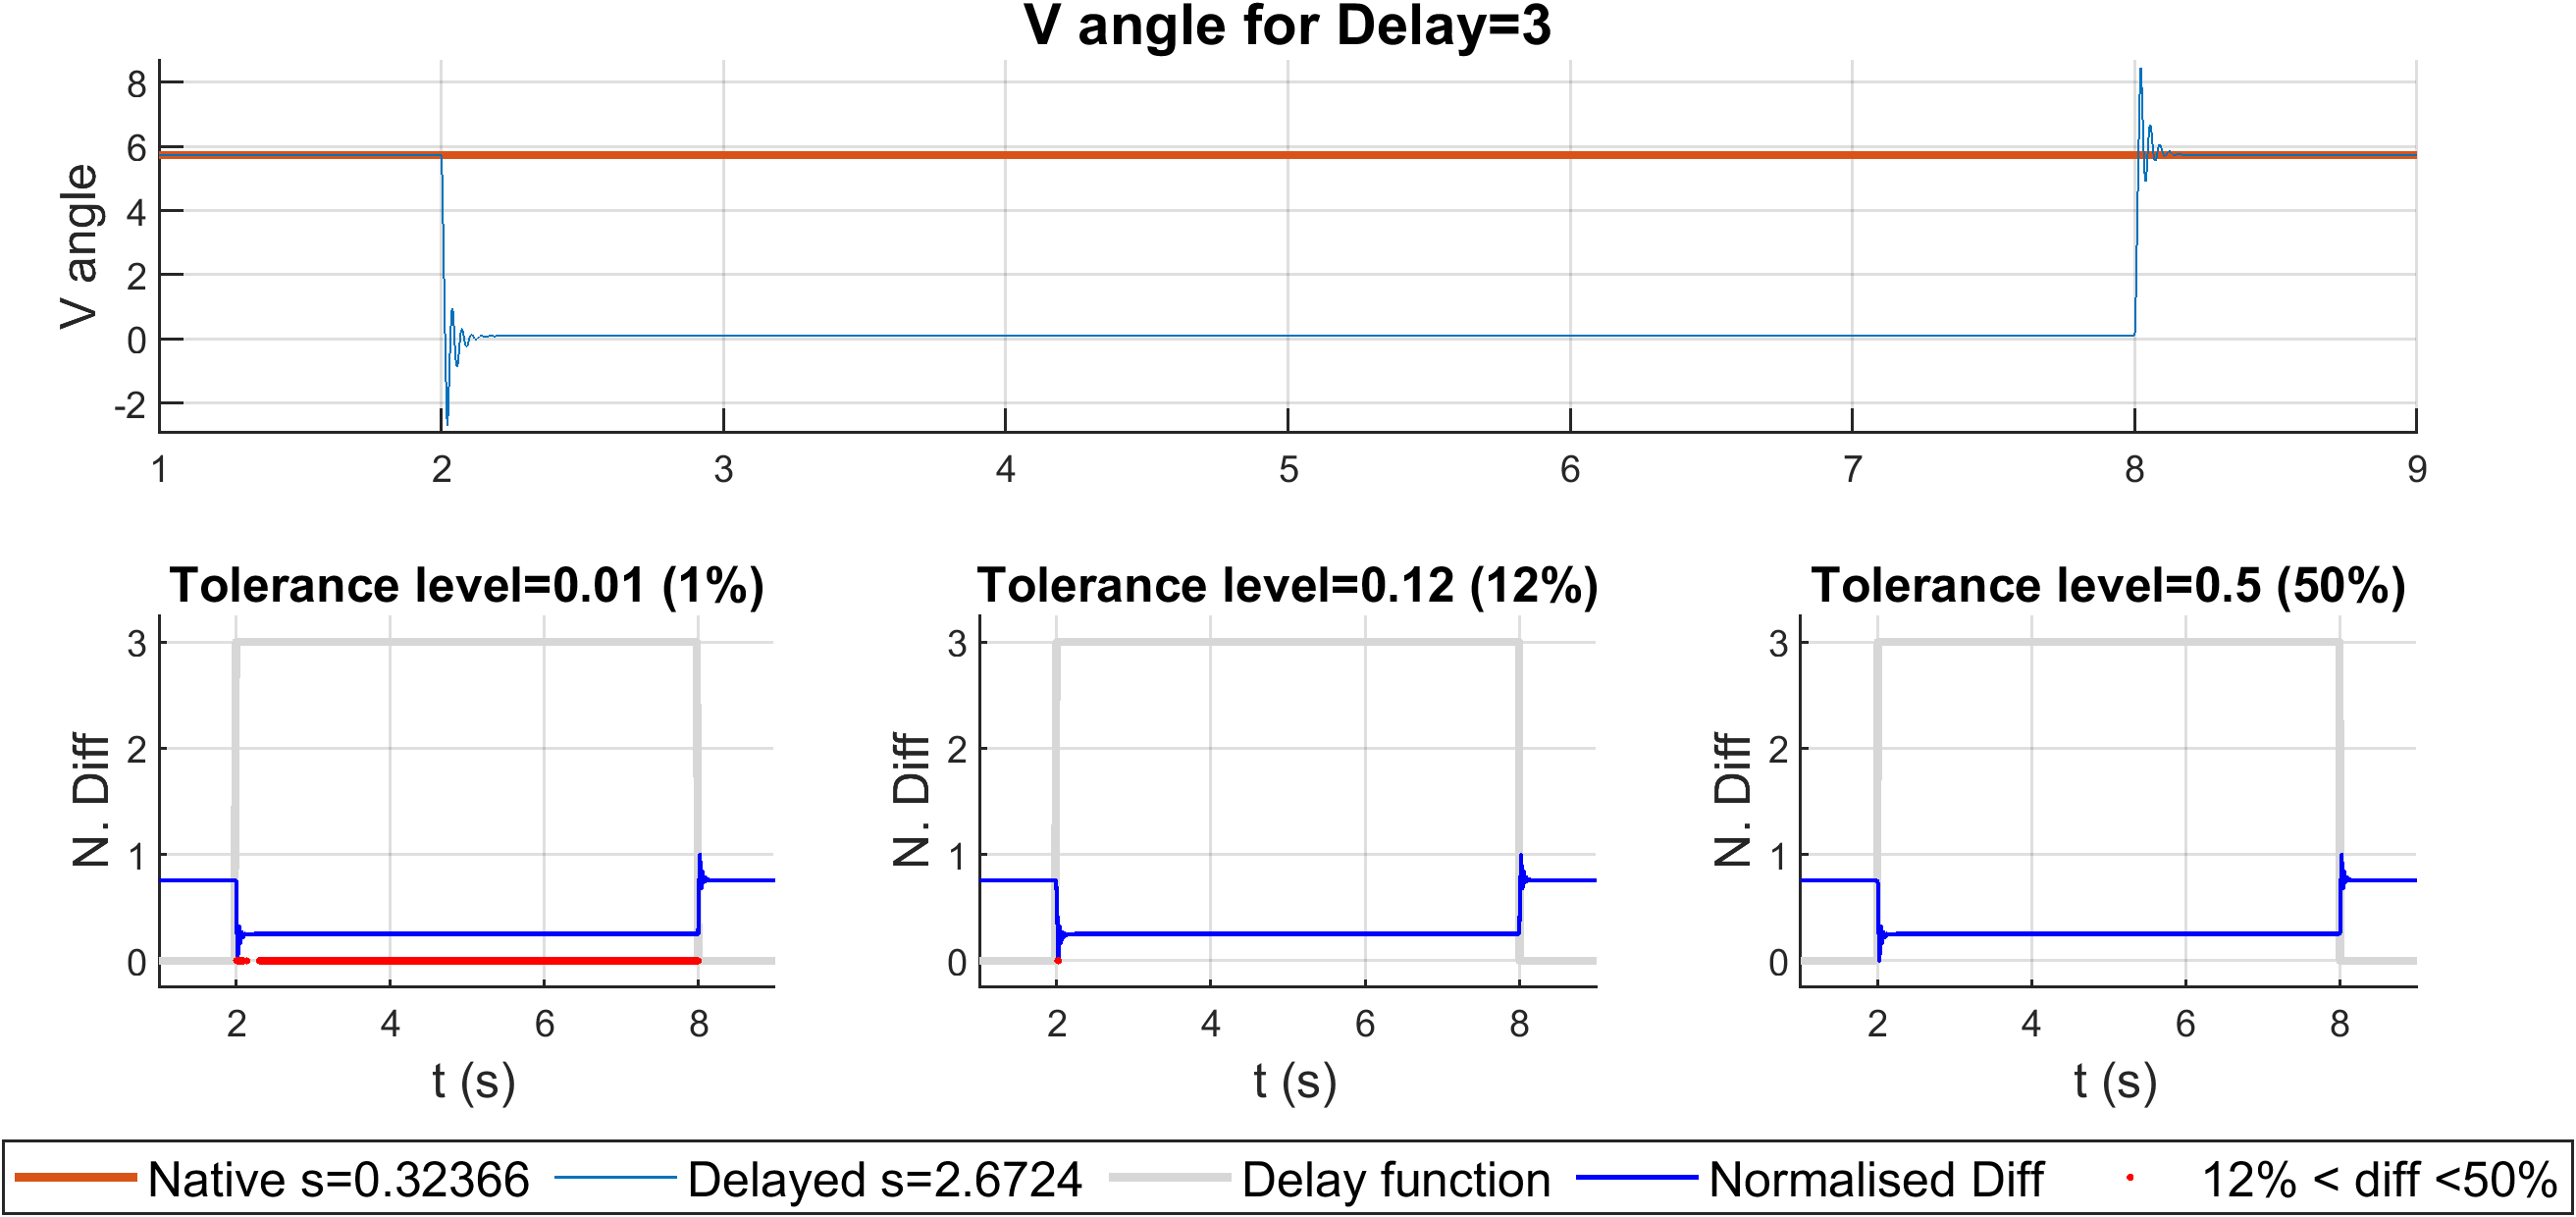
\includegraphics[width=0.95\textwidth]{PMUsim-figures/DelayOf_3/Instant_vAngle.png}}\\
  
      \\ 
   \fbox{  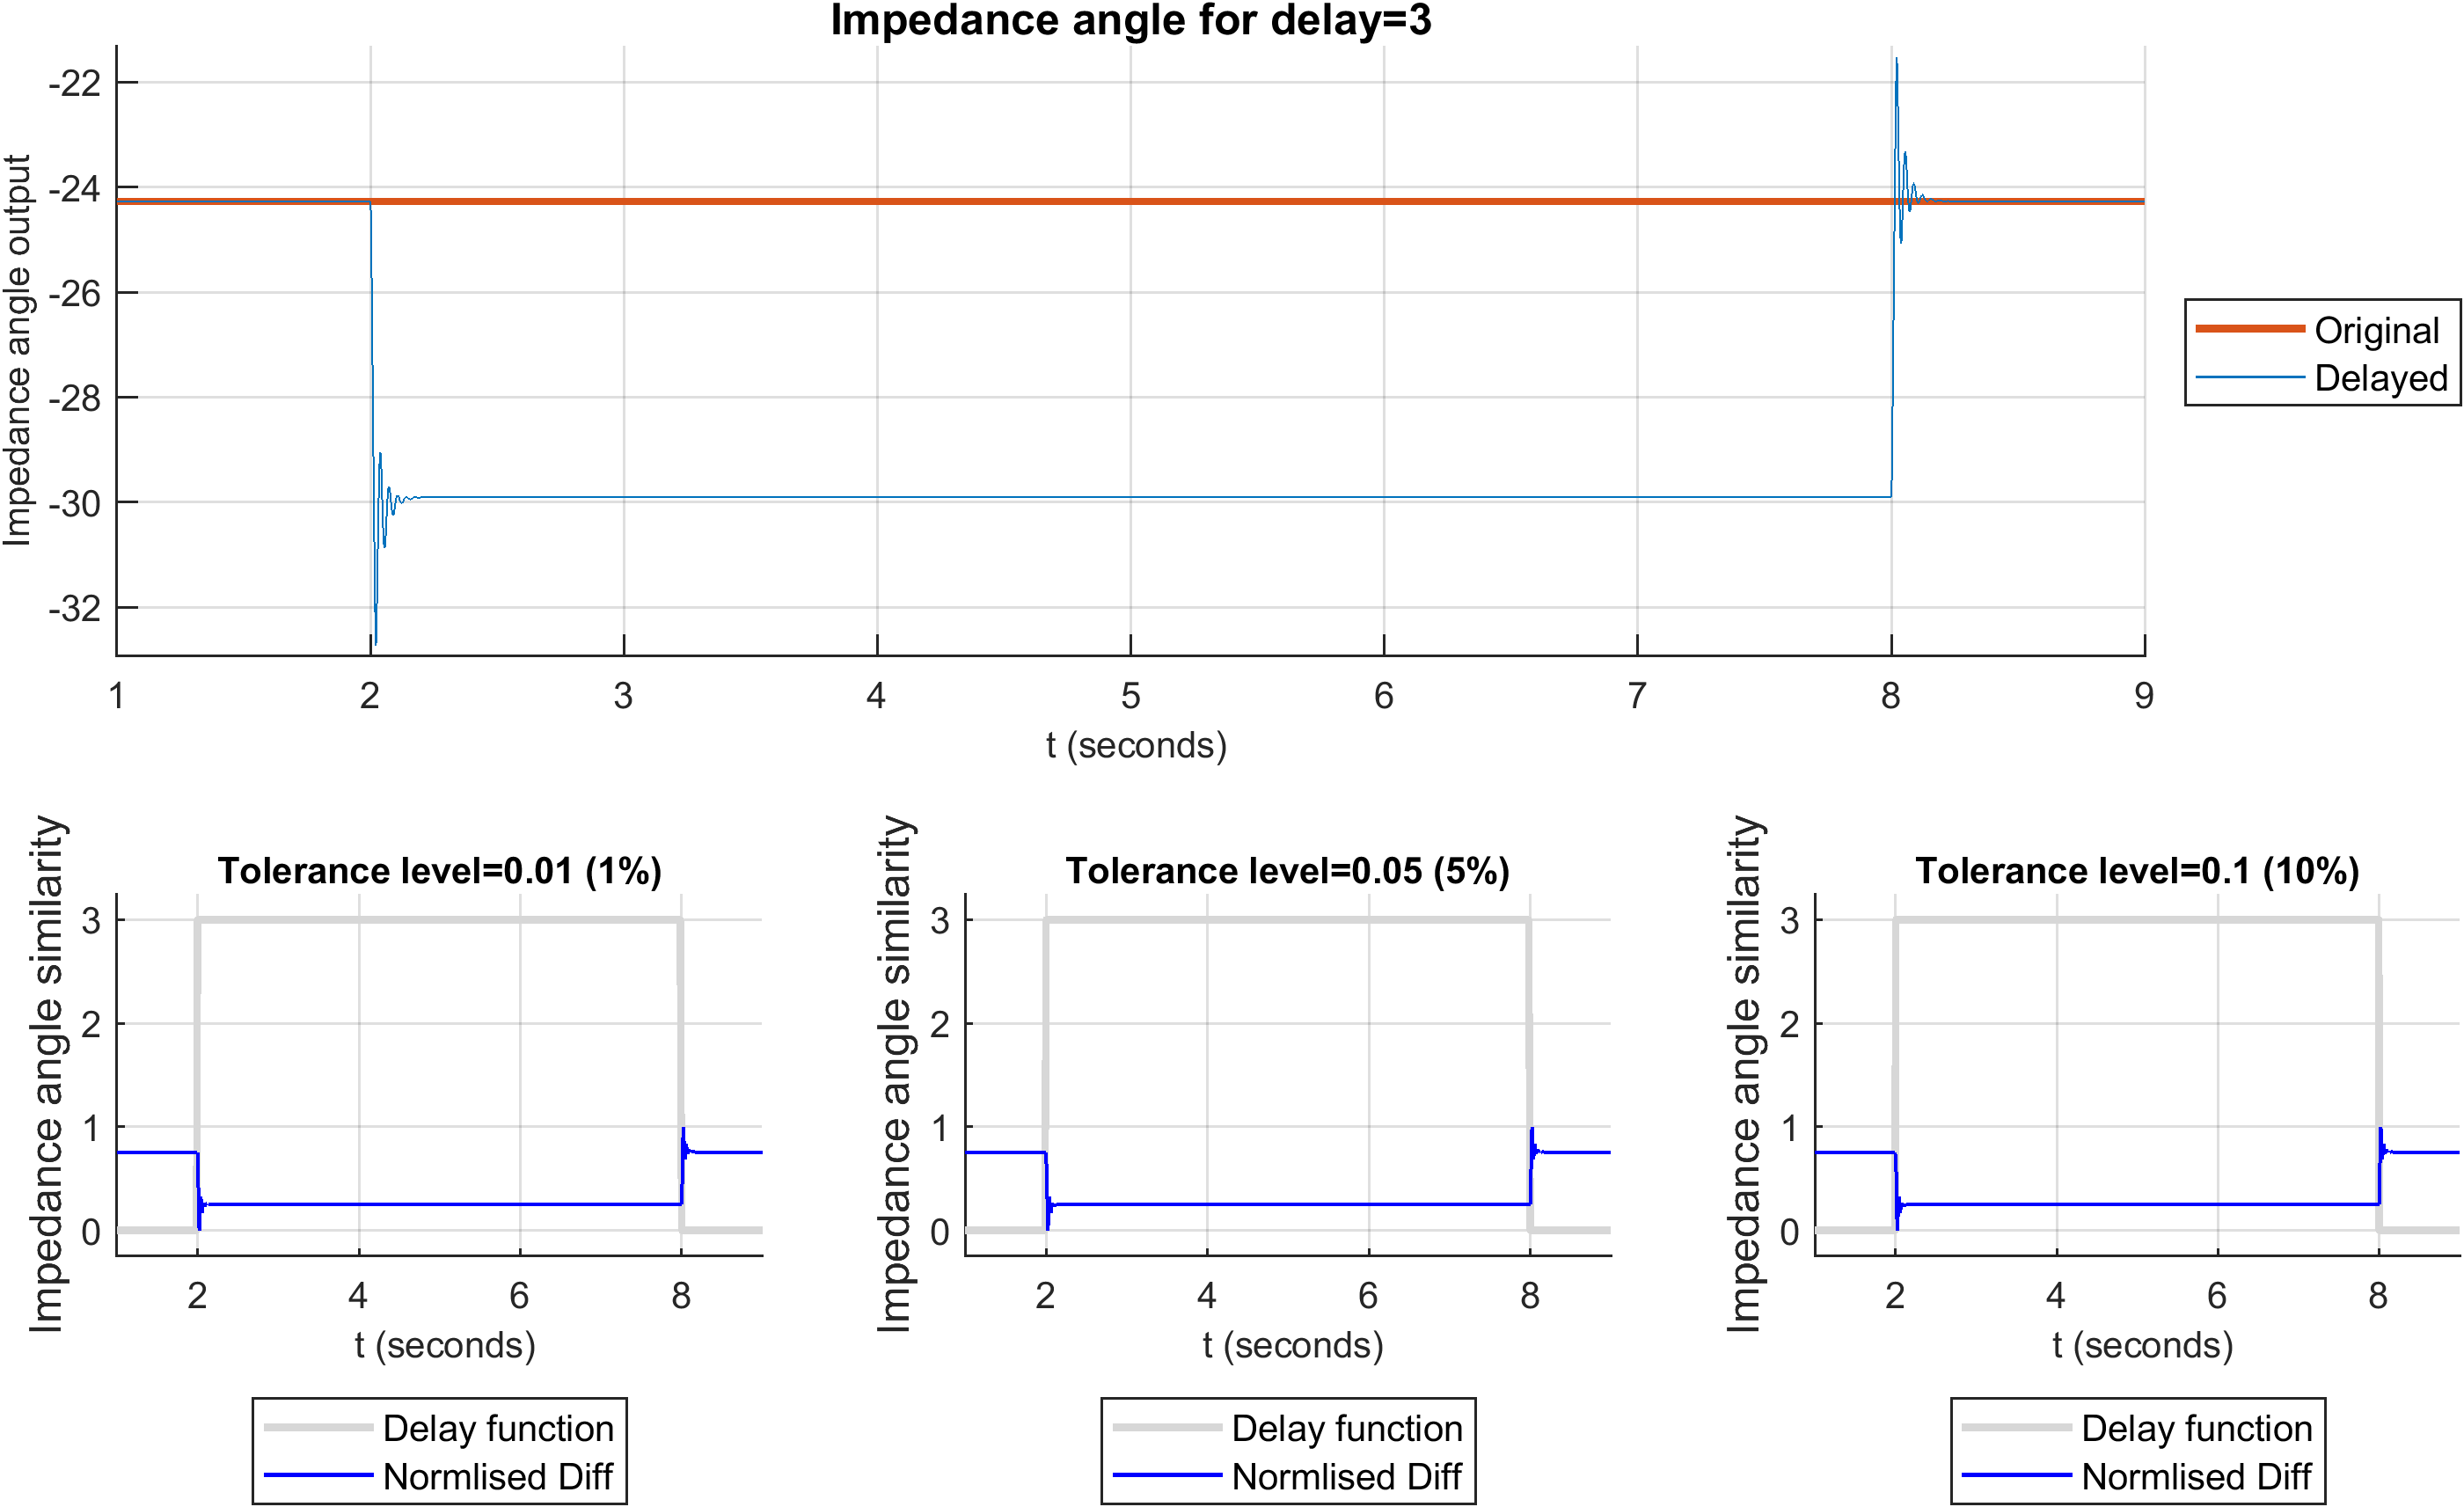
\includegraphics[width=0.95\textwidth]{PMUsim-figures/DelayOf_3/Instant_iAngle.png}}\\
 \label{fig:PMUsim_Three_Angle}
 %\caption{Instant Delay Angle Output for the Delay Level of Three}
  \end{tabular}
\caption[Instant delay of 3: Angle Output]{Results for Angle Output for Instant Delay equal to Three}
 \end{figure}

\newpage 
\subsection{Instant Delay Level of Four}

\begin{small}
     \tcbox[size=normal, standard jigsaw, opacityback=0, boxrule=0pt,halign=justify]{
     Instant Delay Level of Four}{
          \begin{itemize}
         \item      The delayed signal (blue) overlaps the original signal (red), producing a straight line, colored neither red nor blue.
         \item  The blue Normalised diff signal also overlaps the grey delay function.
          \end{itemize} }
\end{small}



\newpage 
\begin{figure}[H]
\begin{tabular}{c}
   \fbox{    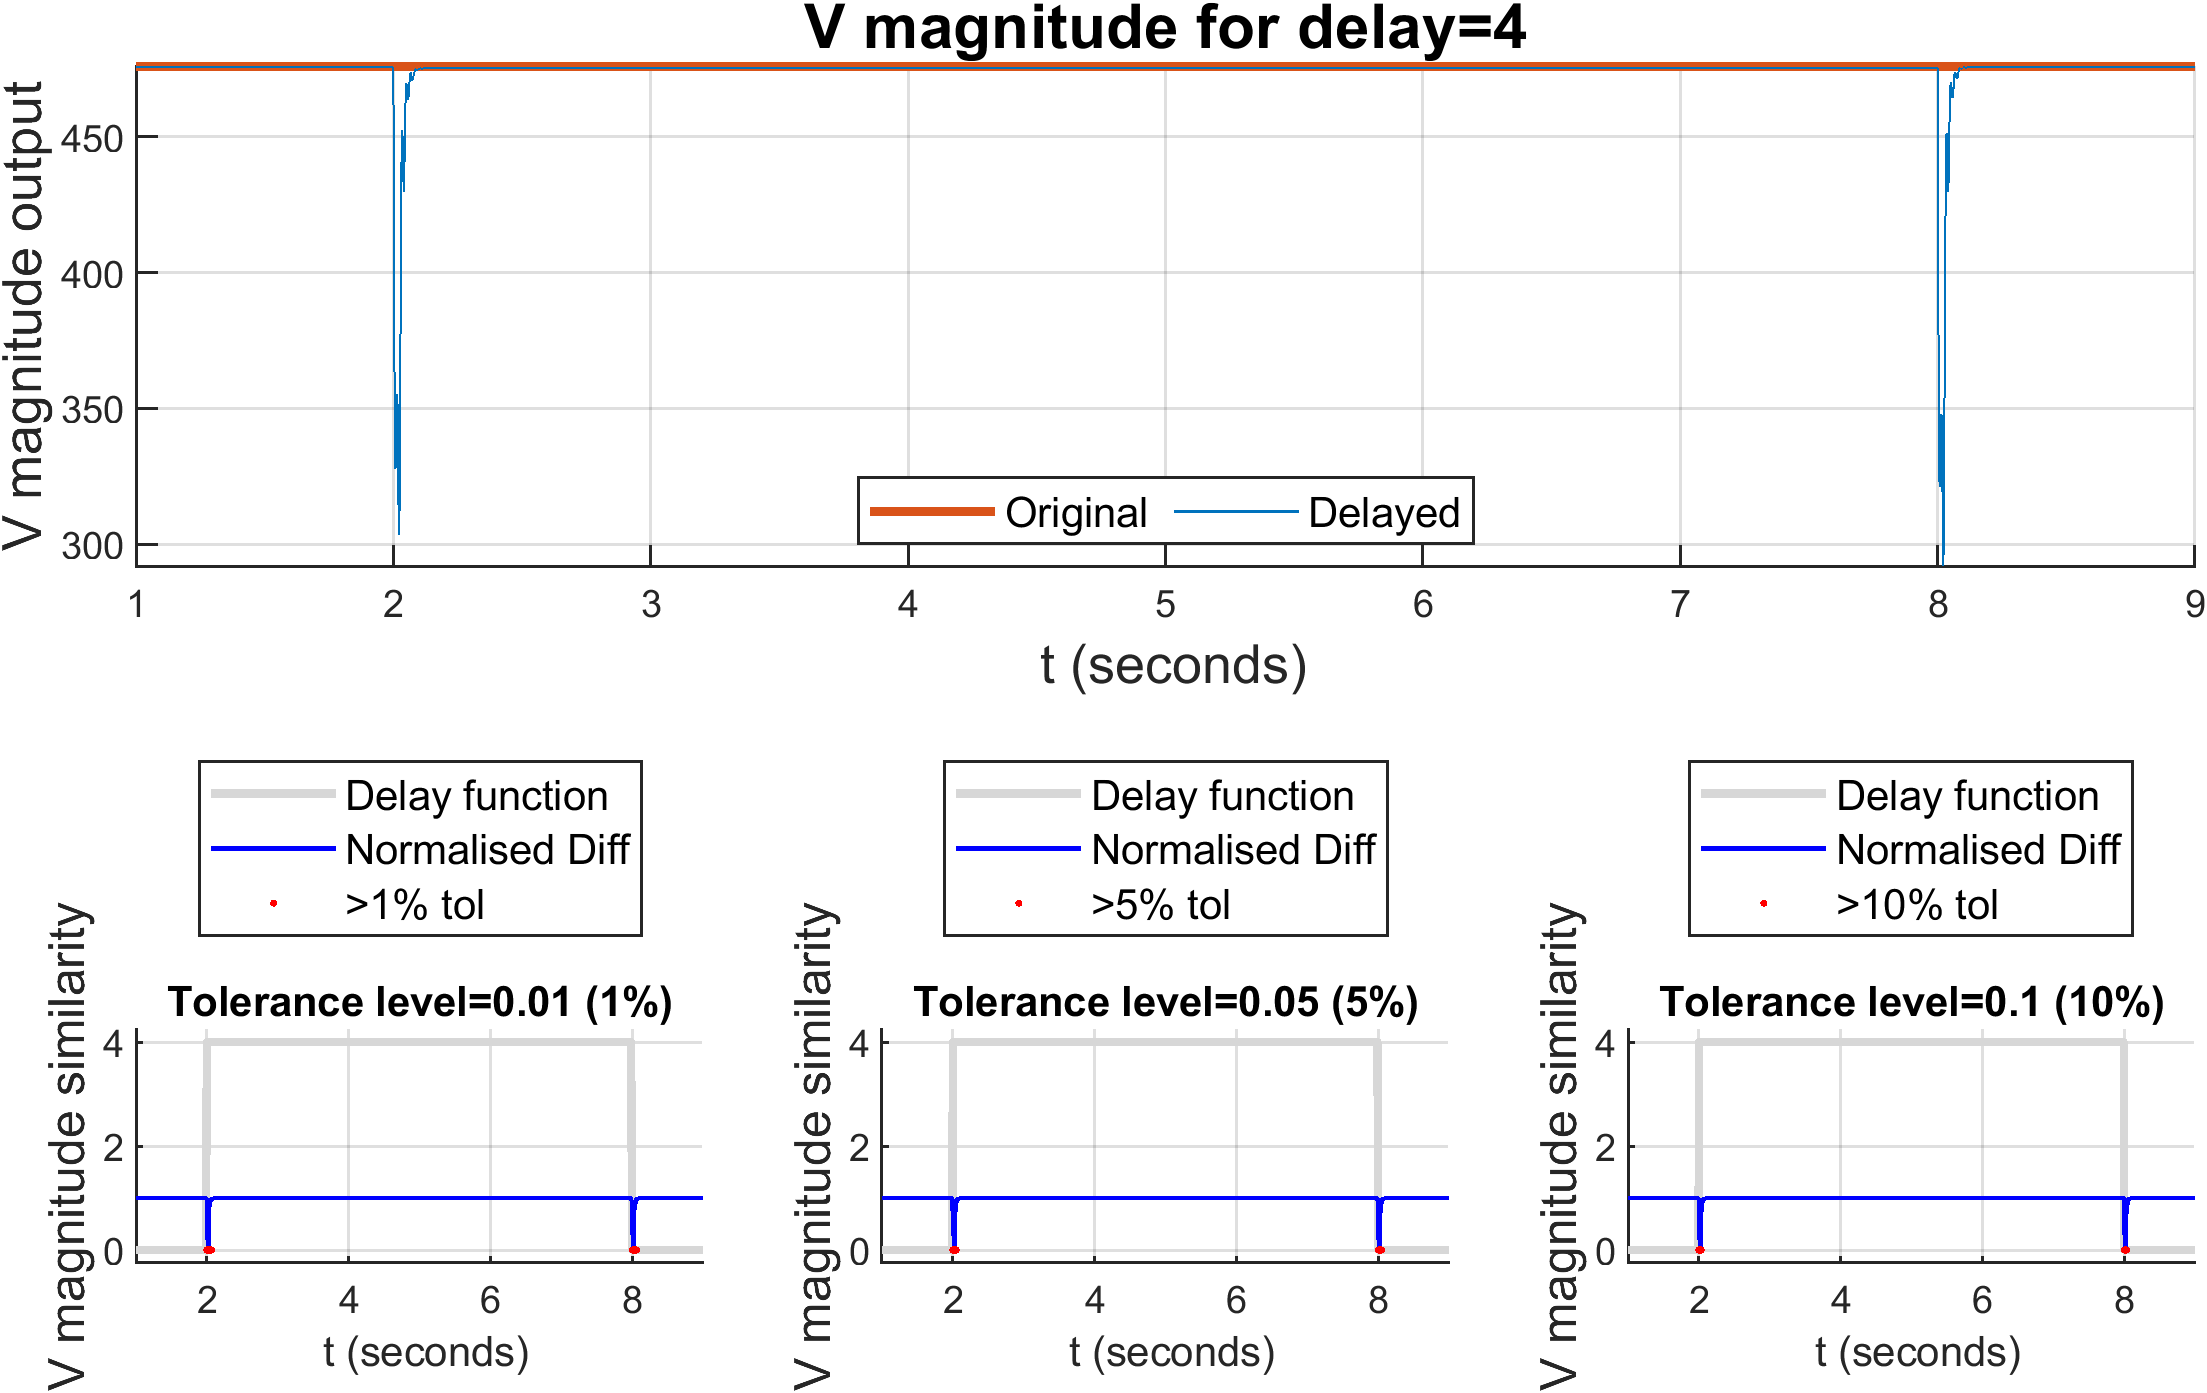
\includegraphics[width=0.95\textwidth]{PMUsim-figures/DelayOf_4/Instant_vMagnitude.png}}\\
    \\ 
    
   \fbox{   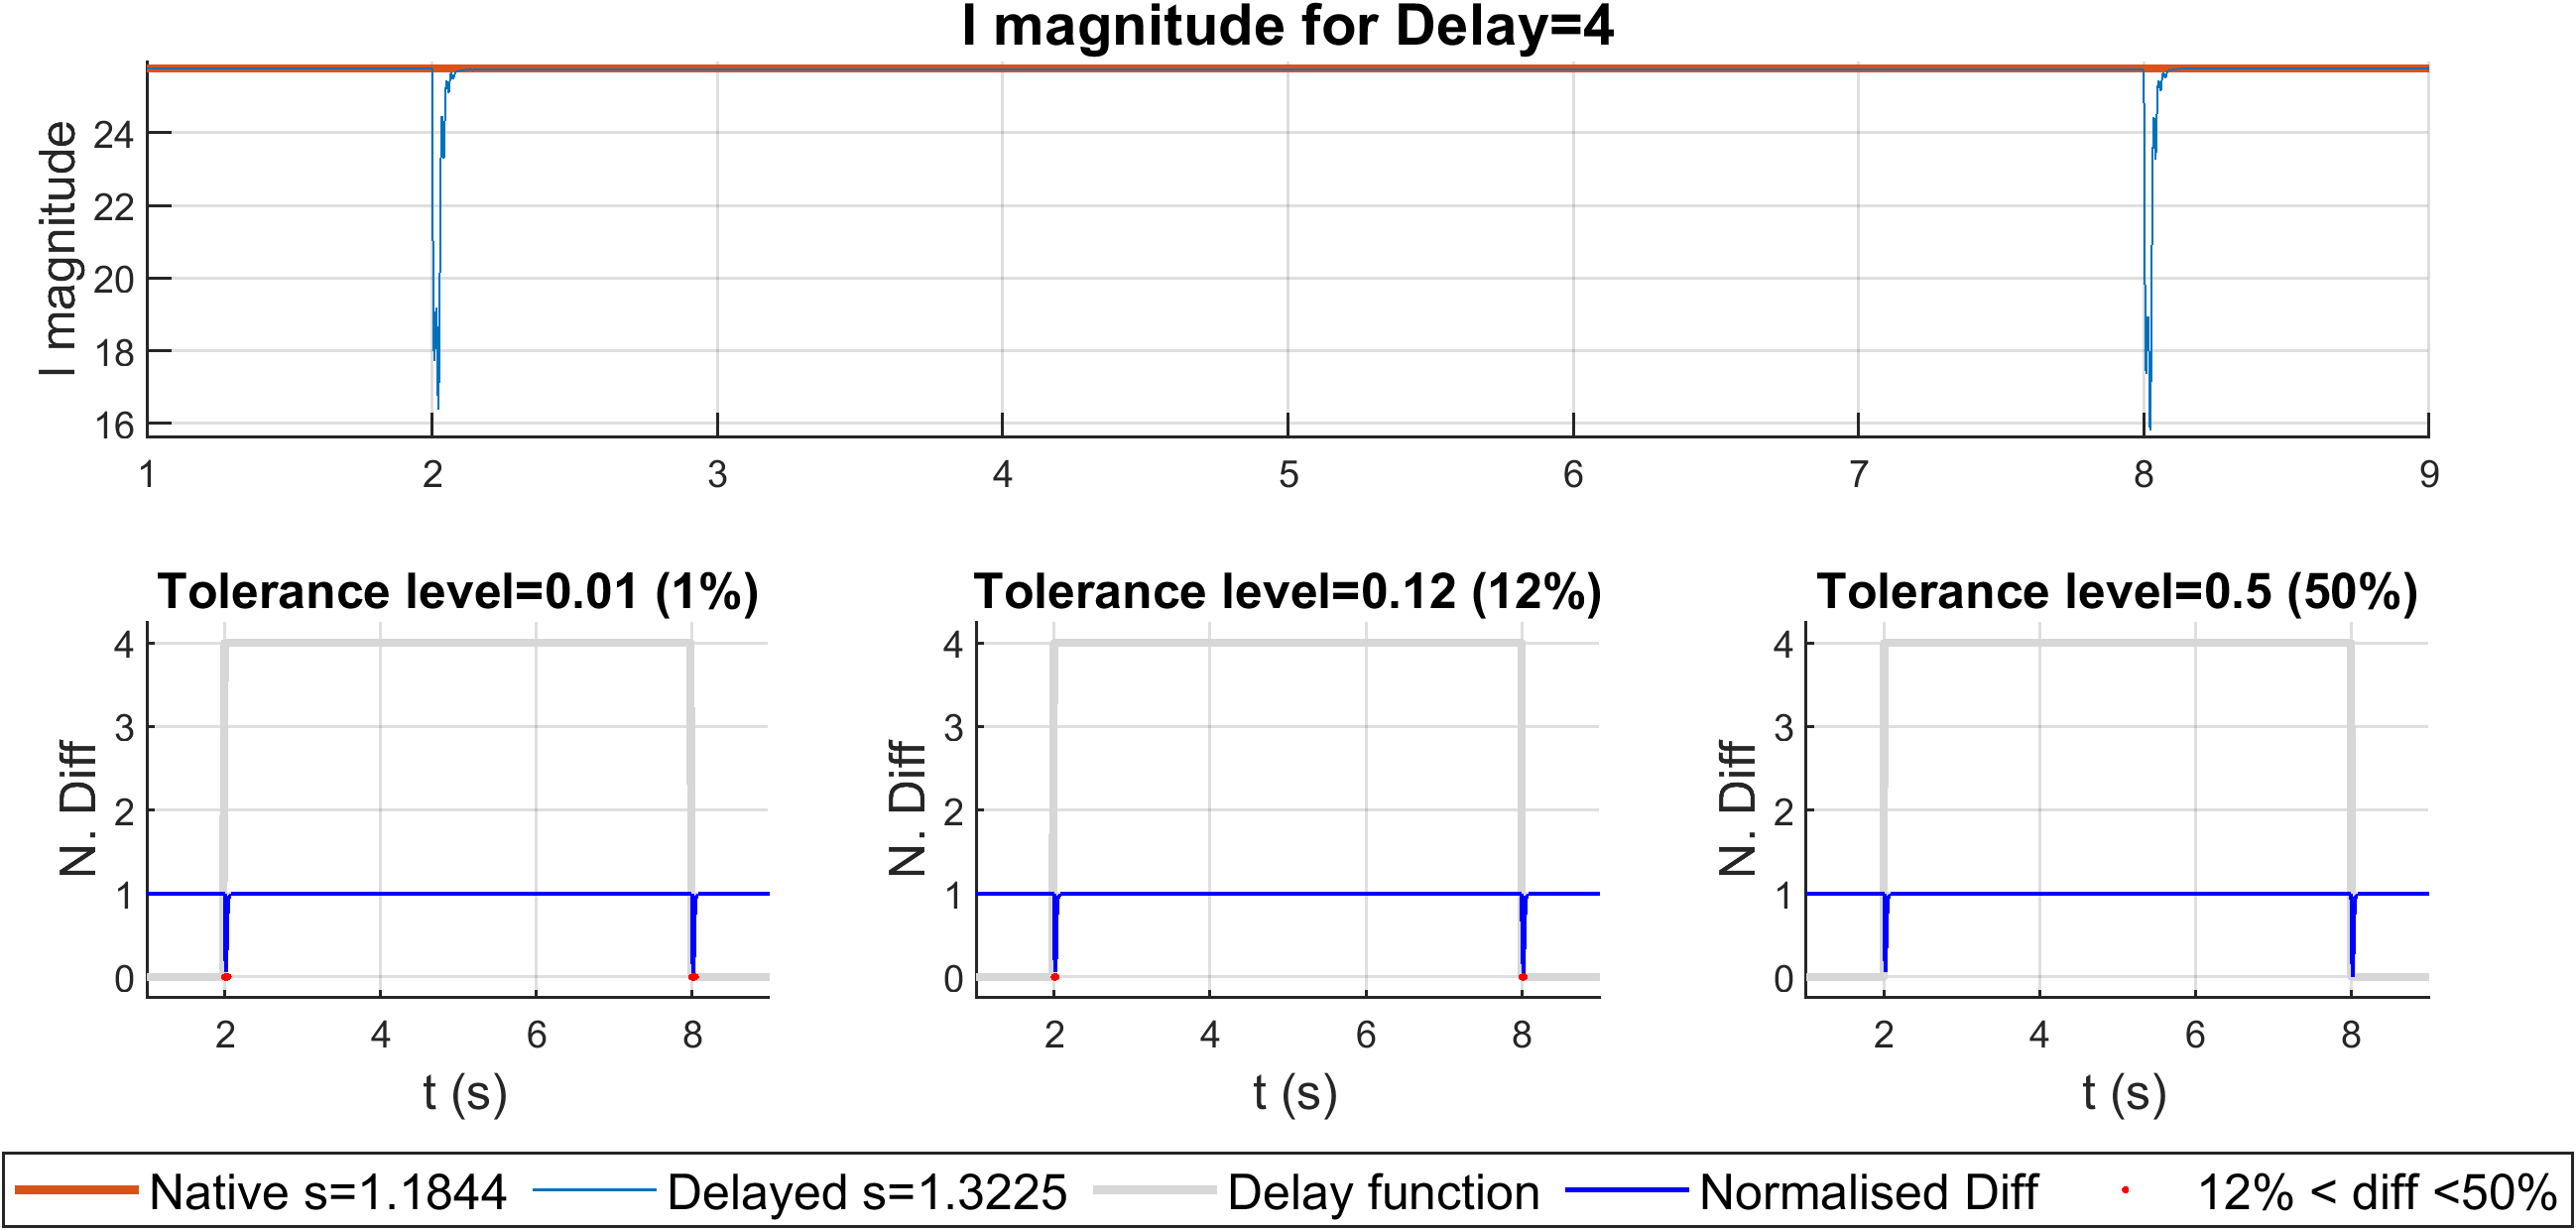
\includegraphics[width=0.95\textwidth]{PMUsim-figures/DelayOf_4/Instant_iMagnitude.png}}\\       
\label{fig:PMUsim_Four_Mag}
 %\caption{Instant Delay Magnitude Output for the Delay Level of Four}
  \end{tabular}
\caption[Instant delay of 4: Magnitude Output]{Results for Magnitude Output for Instant Delay equal to Four}
 \end{figure}


\newpage  
\begin{figure}[H]
\begin{tabular}{c}
   \fbox{     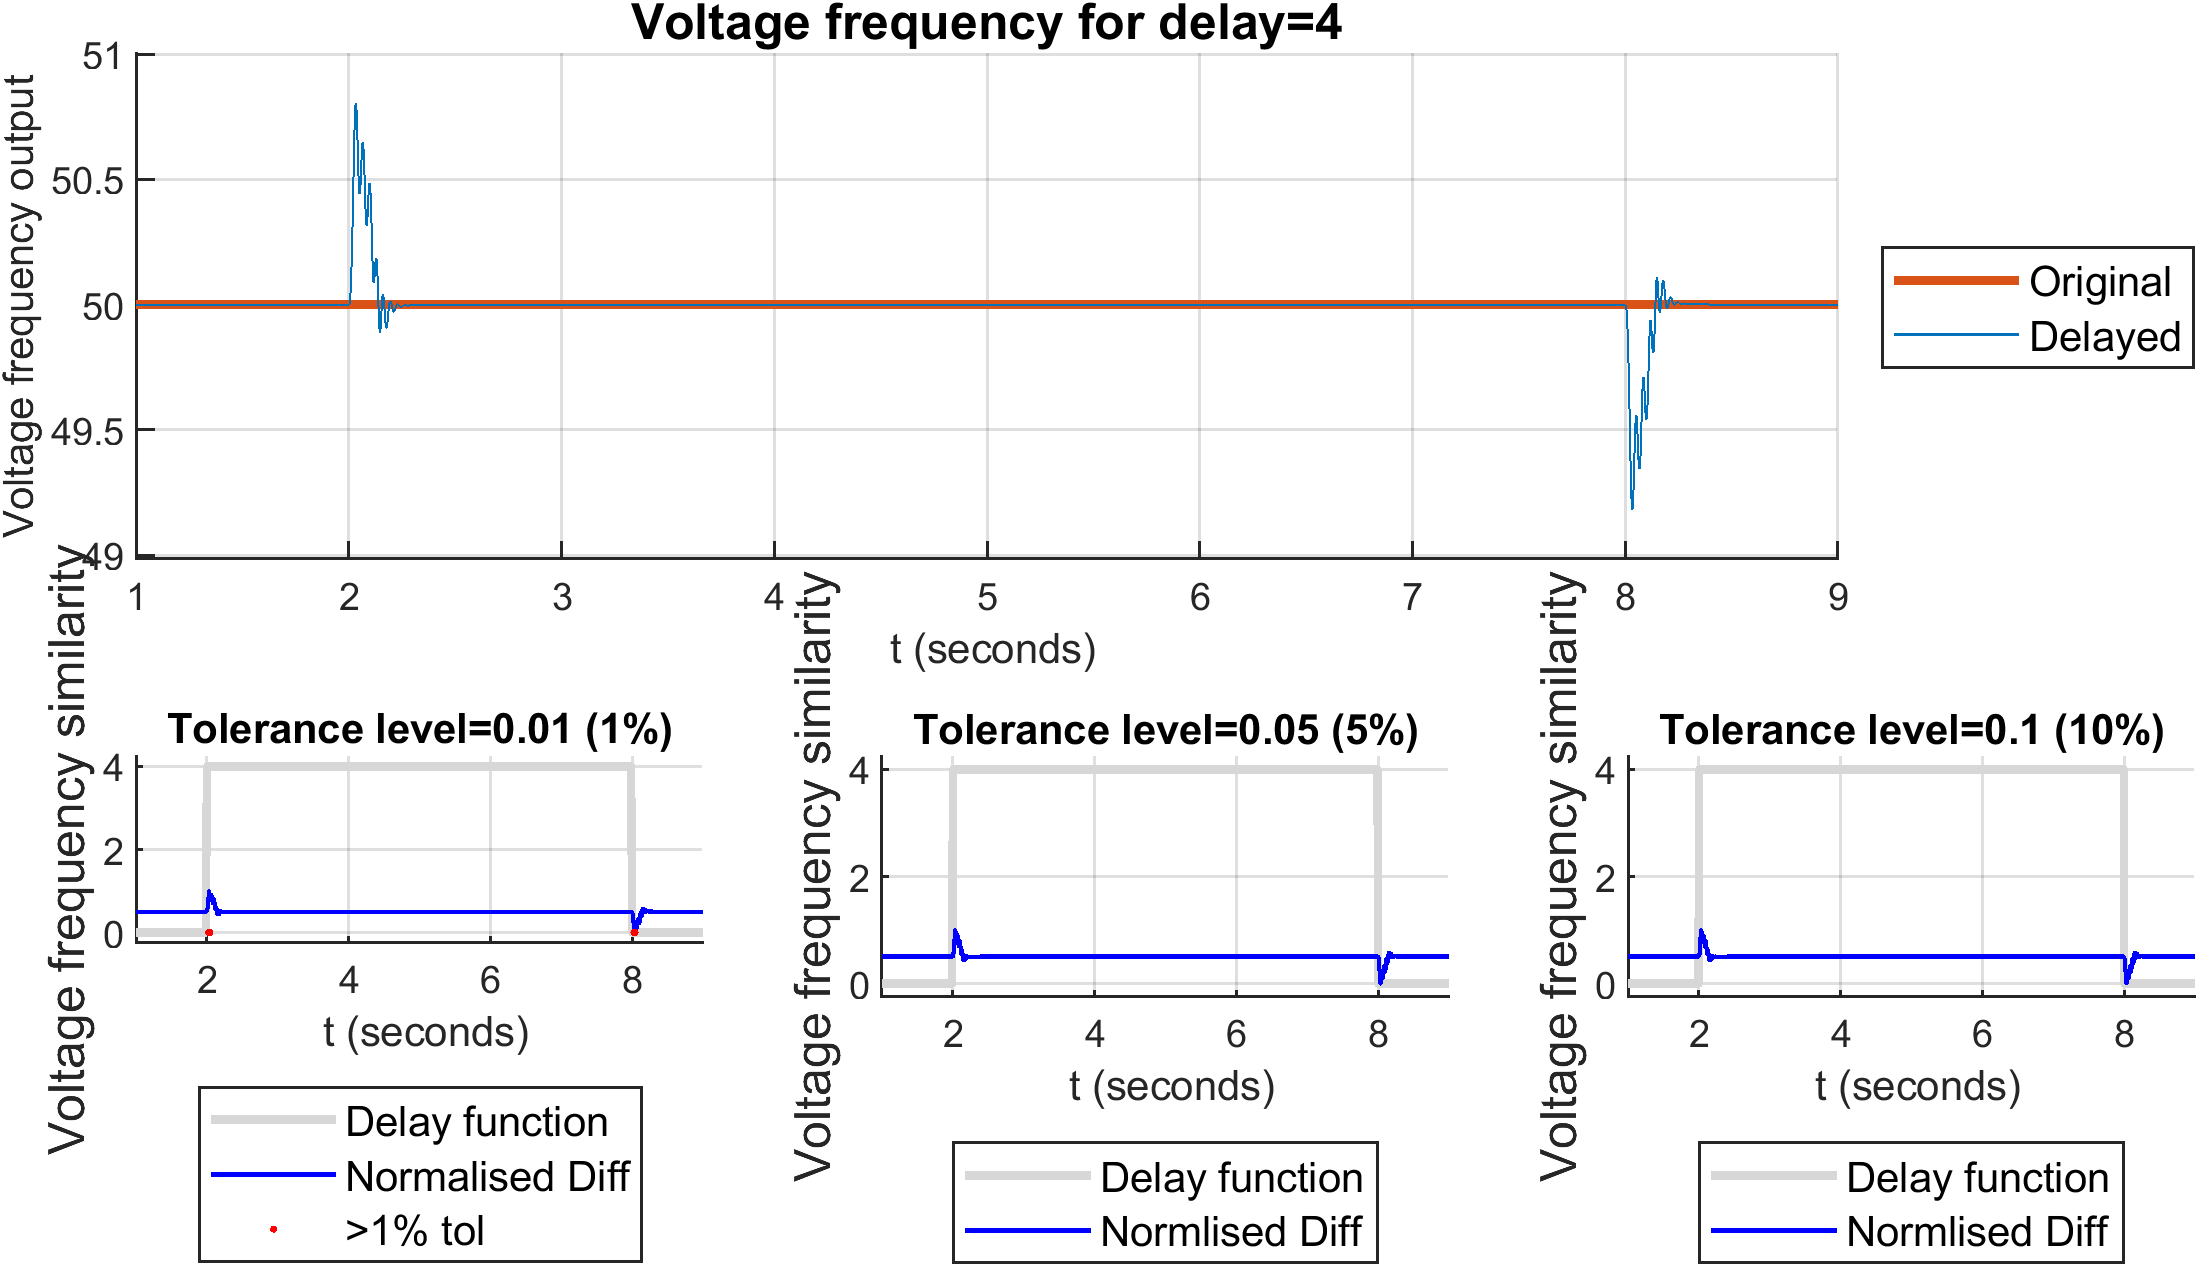
\includegraphics[width=0.95\textwidth]{PMUsim-figures/DelayOf_4/Instant_vFrequency.png}}\\
    \\ 
    
   \fbox{  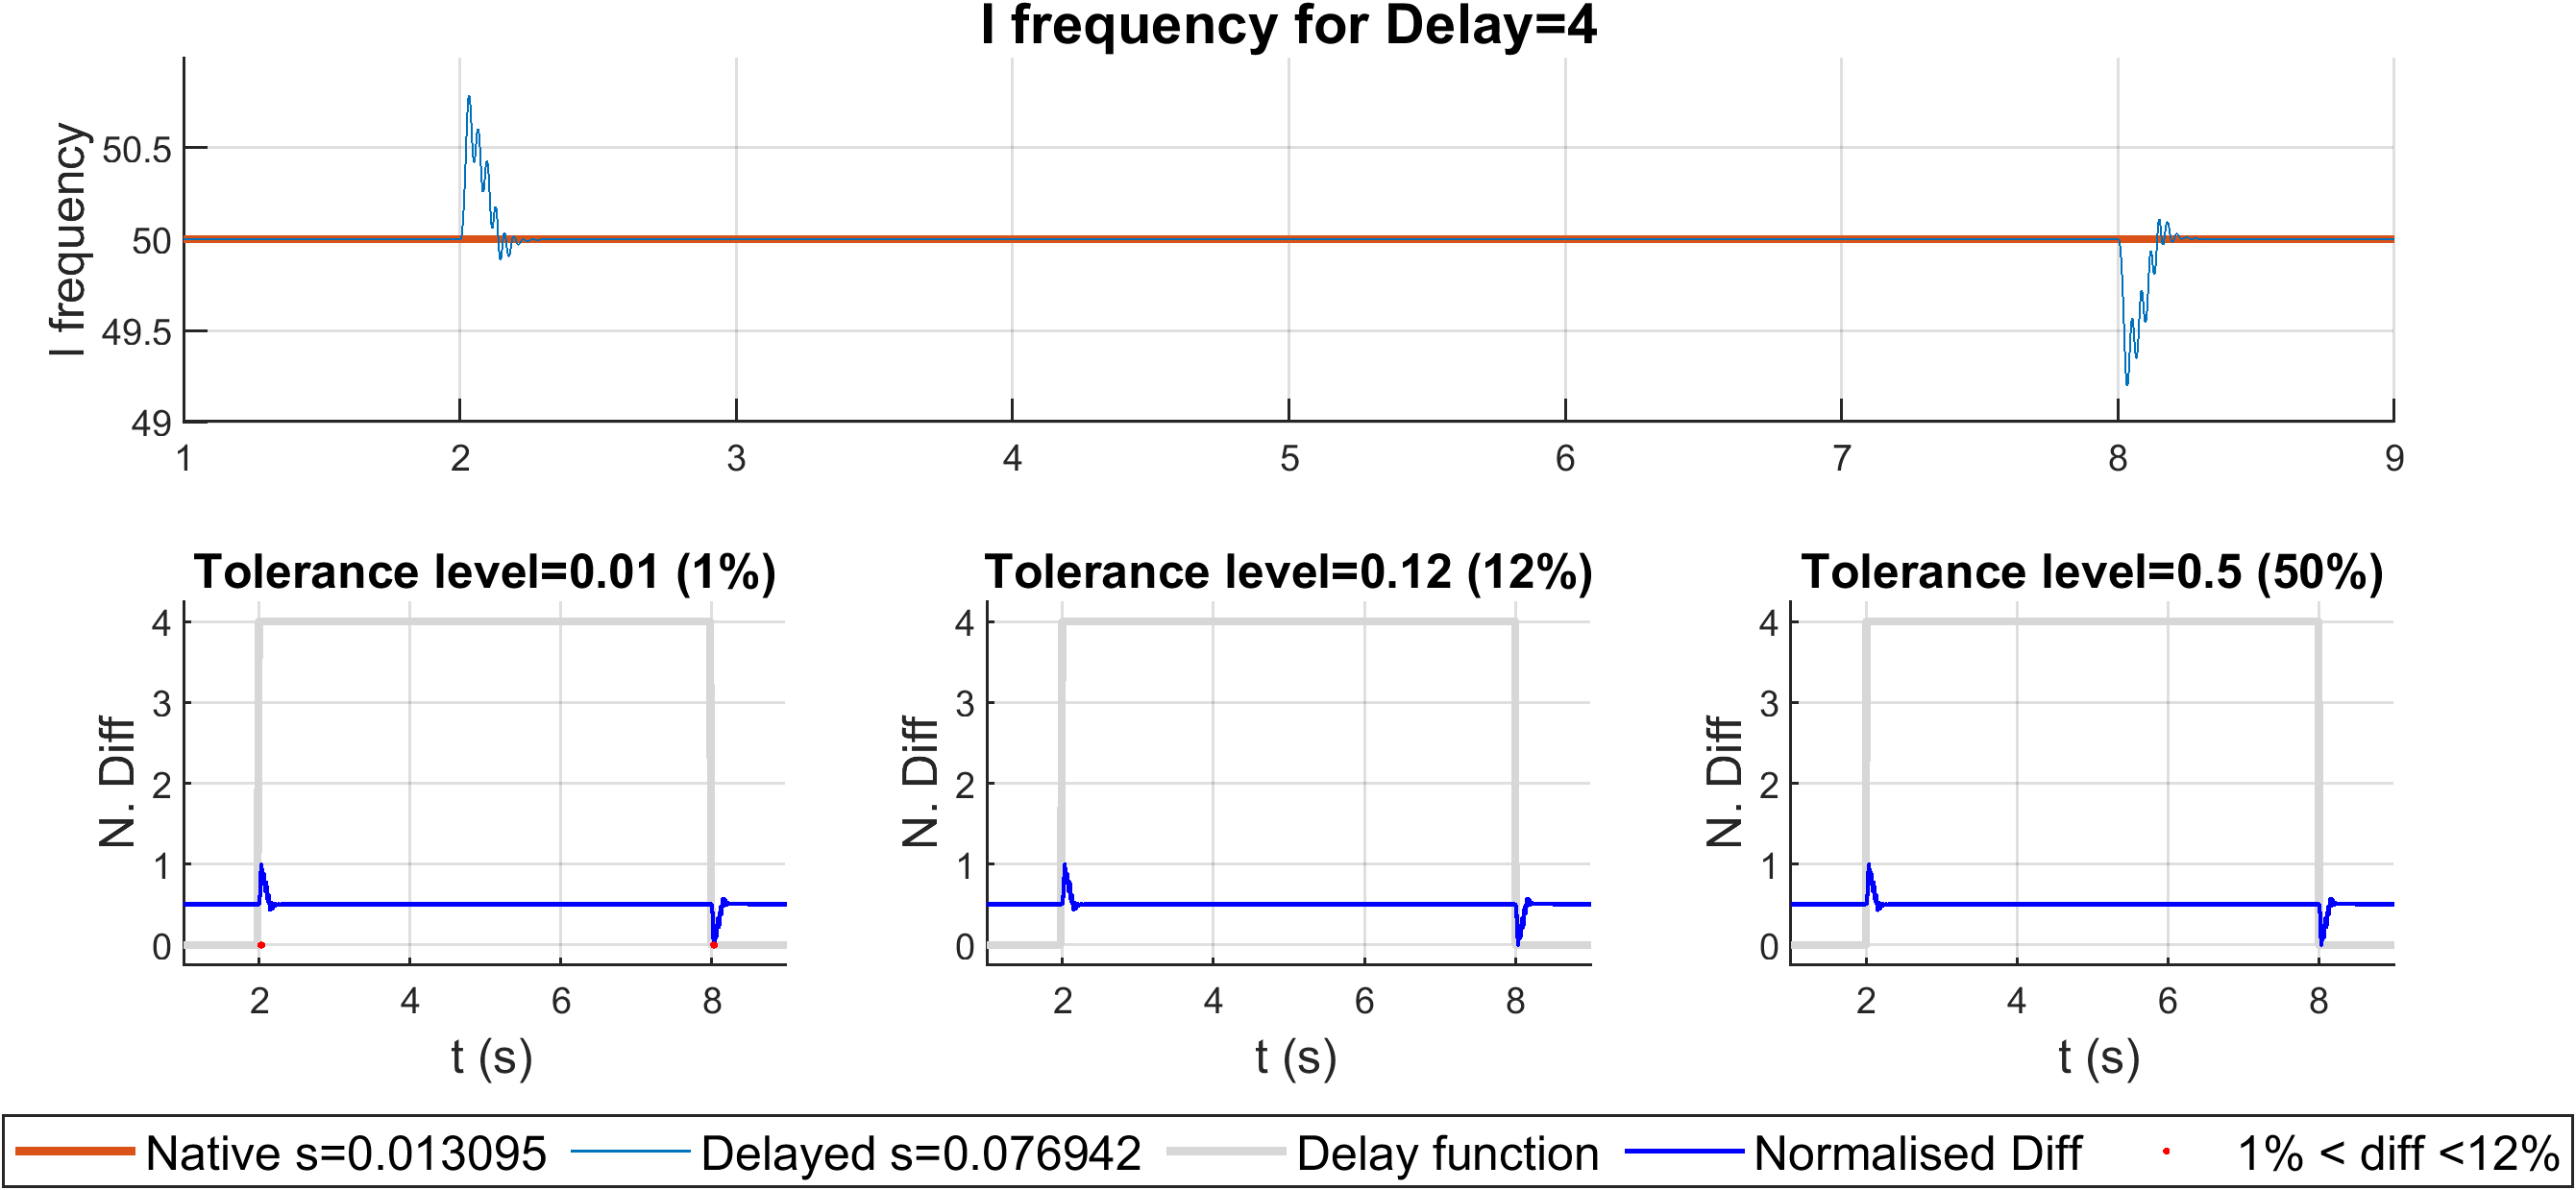
\includegraphics[width=0.95\textwidth]{PMUsim-figures/DelayOf_4/Instant_iFrequency.png}}\\ 
 \label{fig:PMUsim_Four_Freq}
 %\caption{Instant Delay Frequency Output for the Delay Level of Four}
  \end{tabular}
\caption[Instant delay of 4: Frequency Output]{Results for Frequency Output for Instant Delay equal to Four}
 \end{figure}
 

\newpage
\begin{figure}[H]
\begin{tabular}{c}
   \fbox{     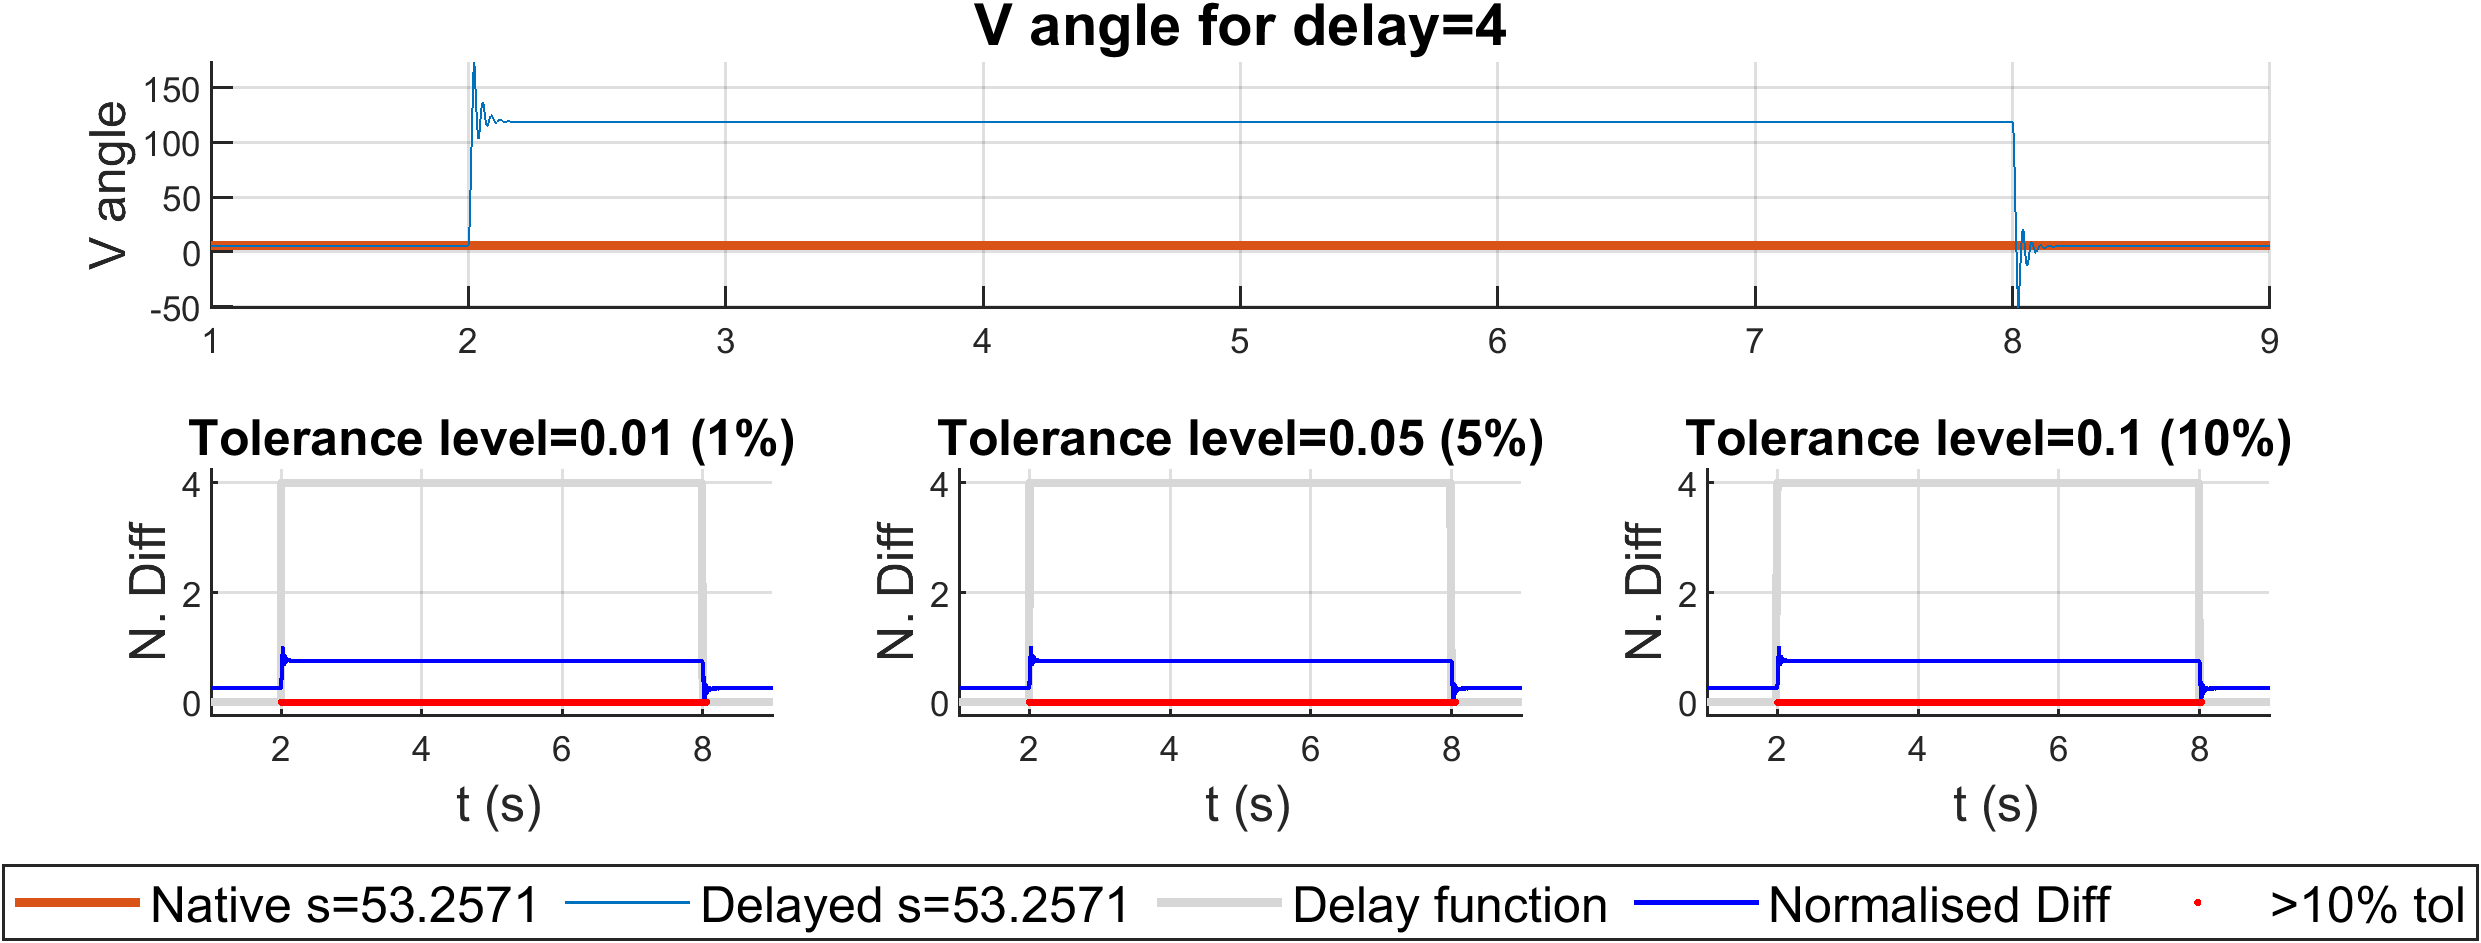
\includegraphics[width=0.95\textwidth]{PMUsim-figures/DelayOf_4/Instant_vAngle.png}}\\
    \\ 
    
   \fbox{  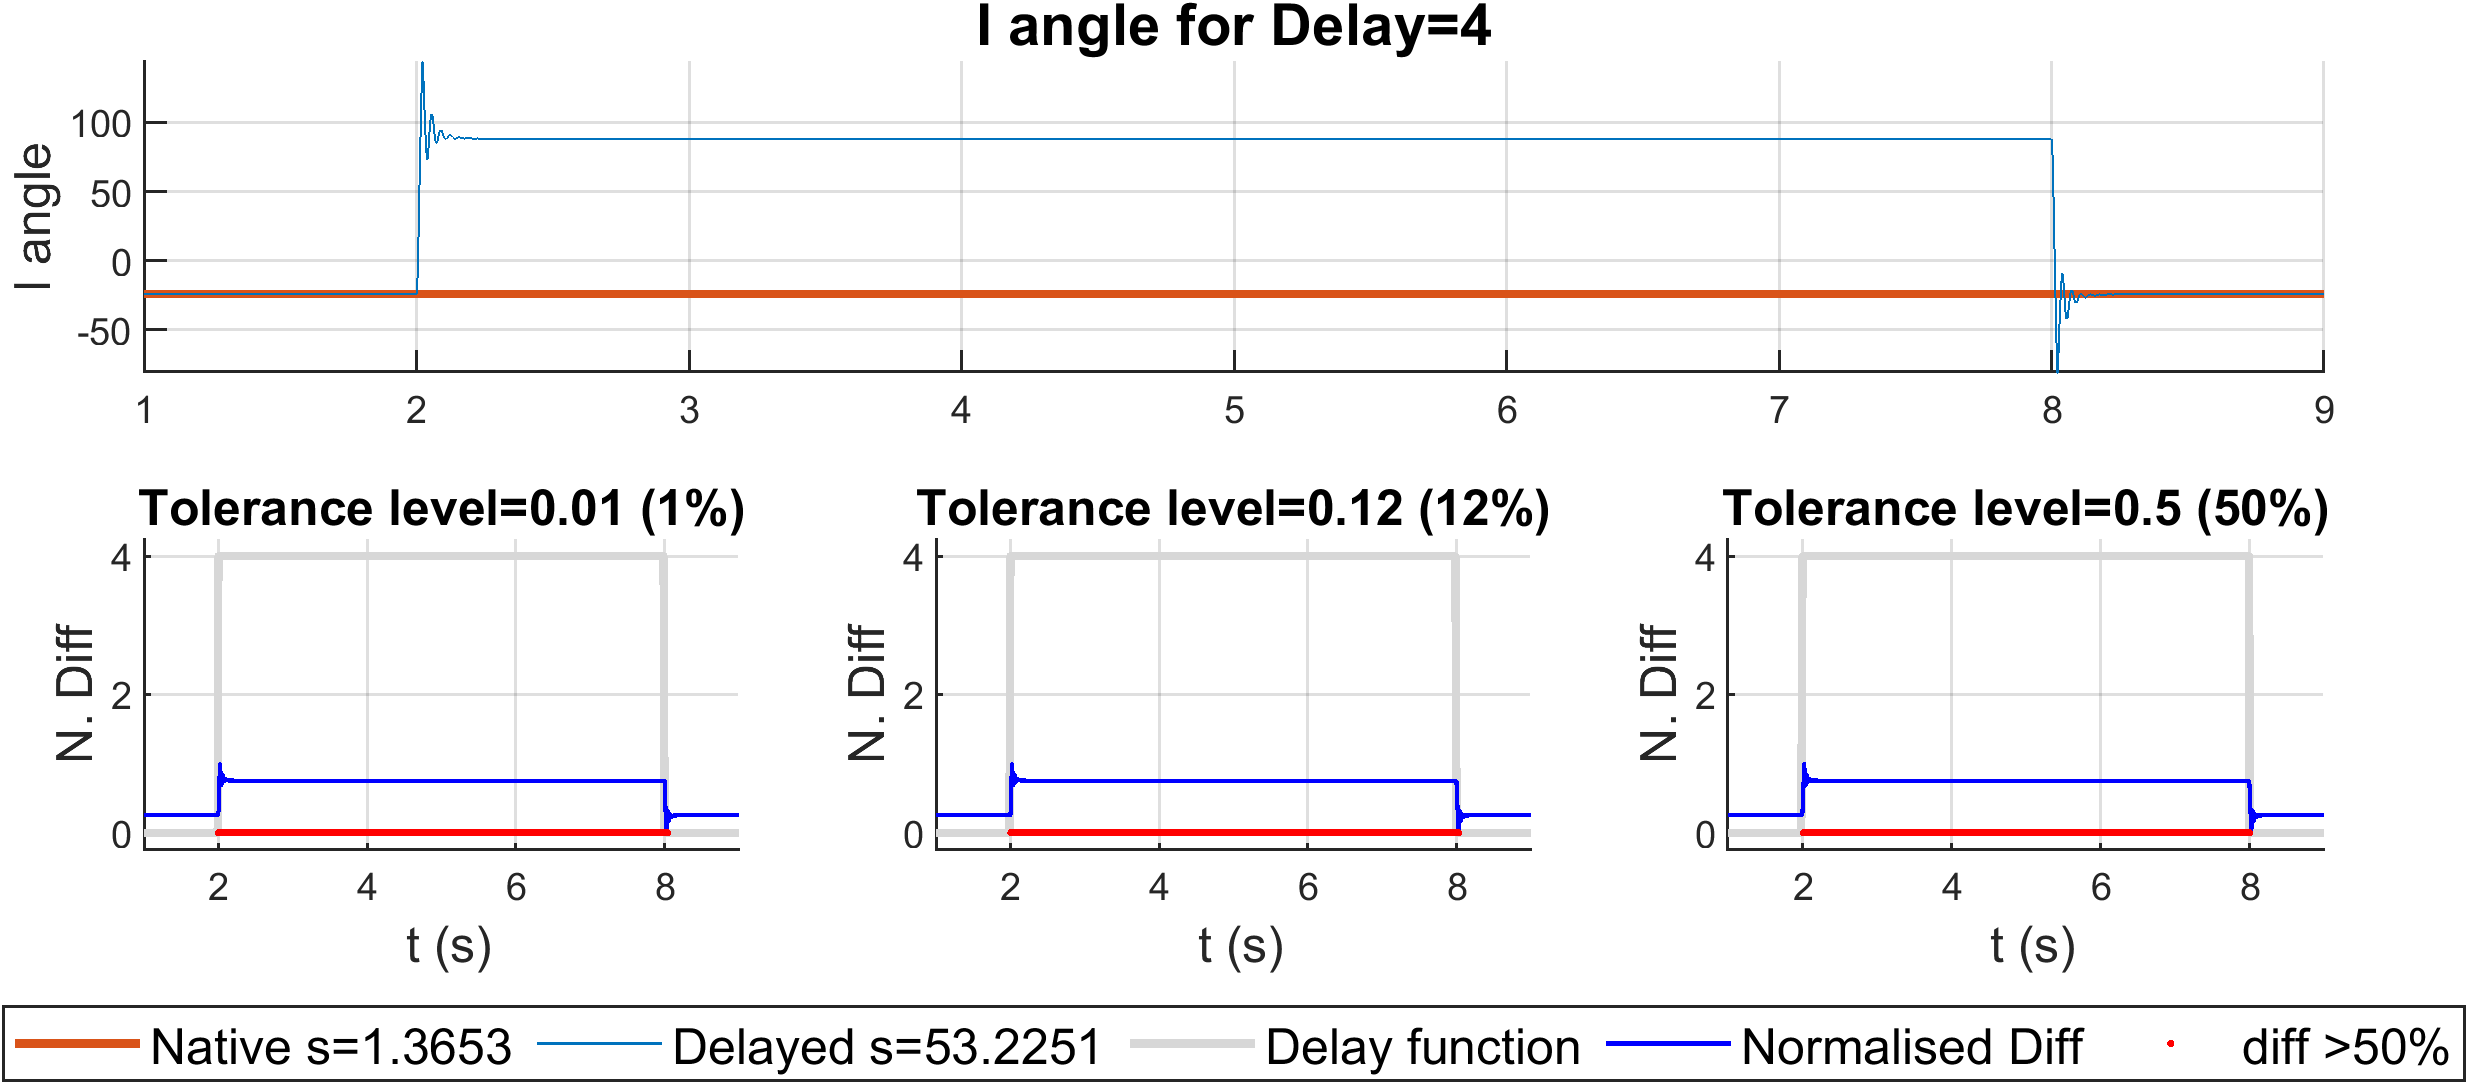
\includegraphics[width=0.95\textwidth]{PMUsim-figures/DelayOf_4/Instant_iAngle.png}}\\
 \label{fig:PMUsim_Four_Angle}
 %\caption{Instant Delay Angle Output for the Delay Level of Four}
  \end{tabular}
\caption[Instant delay of 4: Angle Output]{Results for Angle Output for Instant Delay equal to Four}
 \end{figure}

\newpage 
 \subsection{Instant Delay Level of Five}

\begin{small}
     \tcbox[size=normal, standard jigsaw, opacityback=0, boxrule=0pt,halign=justify]{
     Instant Delay Level of Five}{
          \begin{itemize}
         \item      The delayed signal (blue) overlaps the original signal (red), producing a straight line, colored neither red nor blue.
         \item  The blue Normalised diff signal also overlaps the grey delay function.
          \end{itemize} }
\end{small}



\newpage 
\begin{figure}[H]
\begin{tabular}{c}
   \fbox{     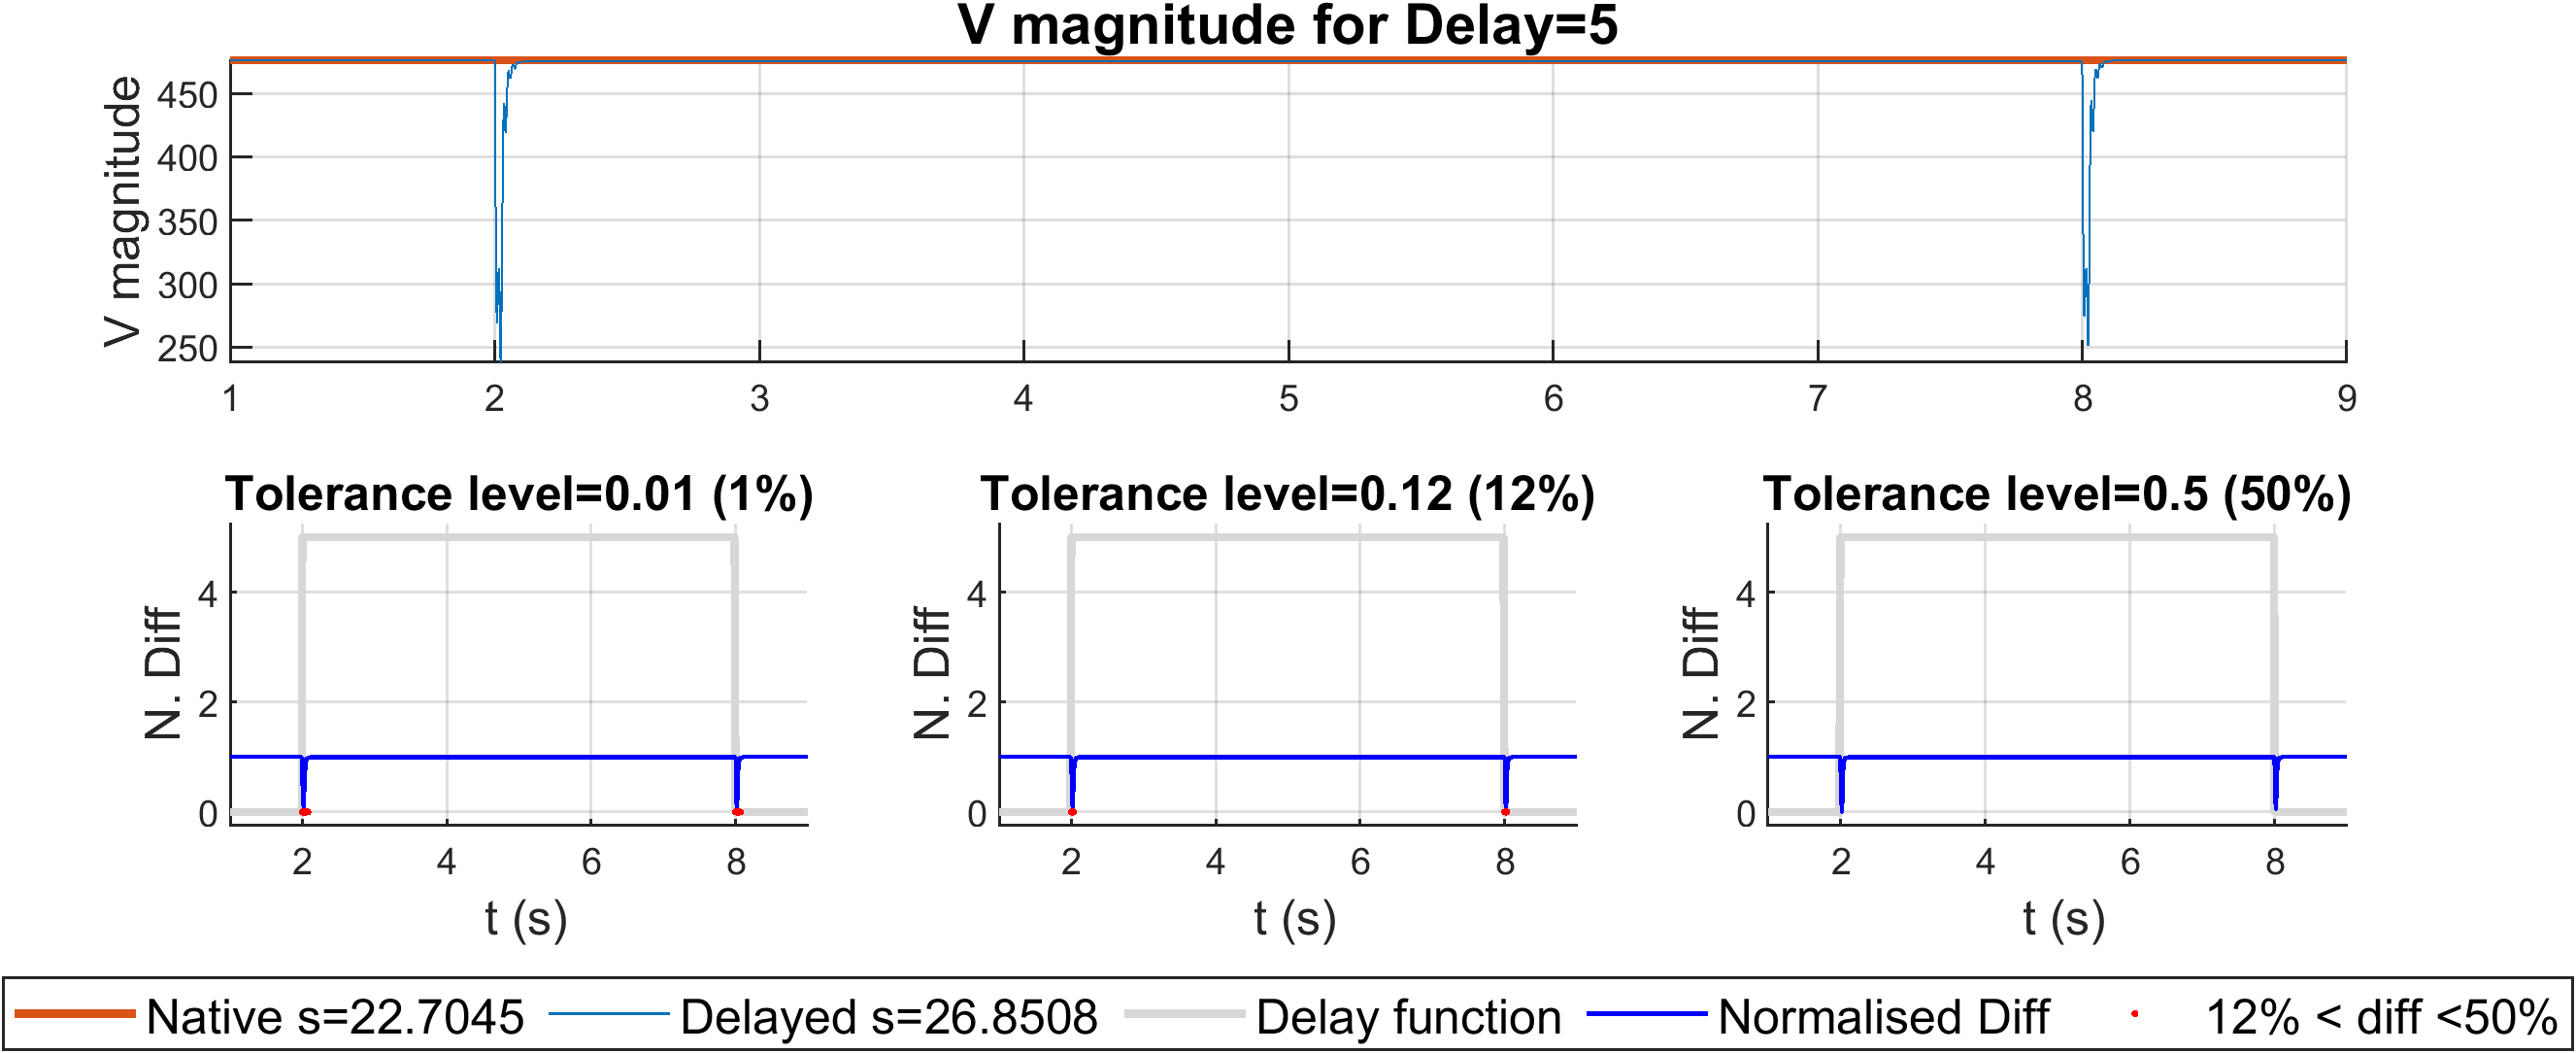
\includegraphics[width=0.95\textwidth]{PMUsim-figures/DelayOf_5/Instant_vMagnitude.png}}\\
    \\ 
    
   \fbox{   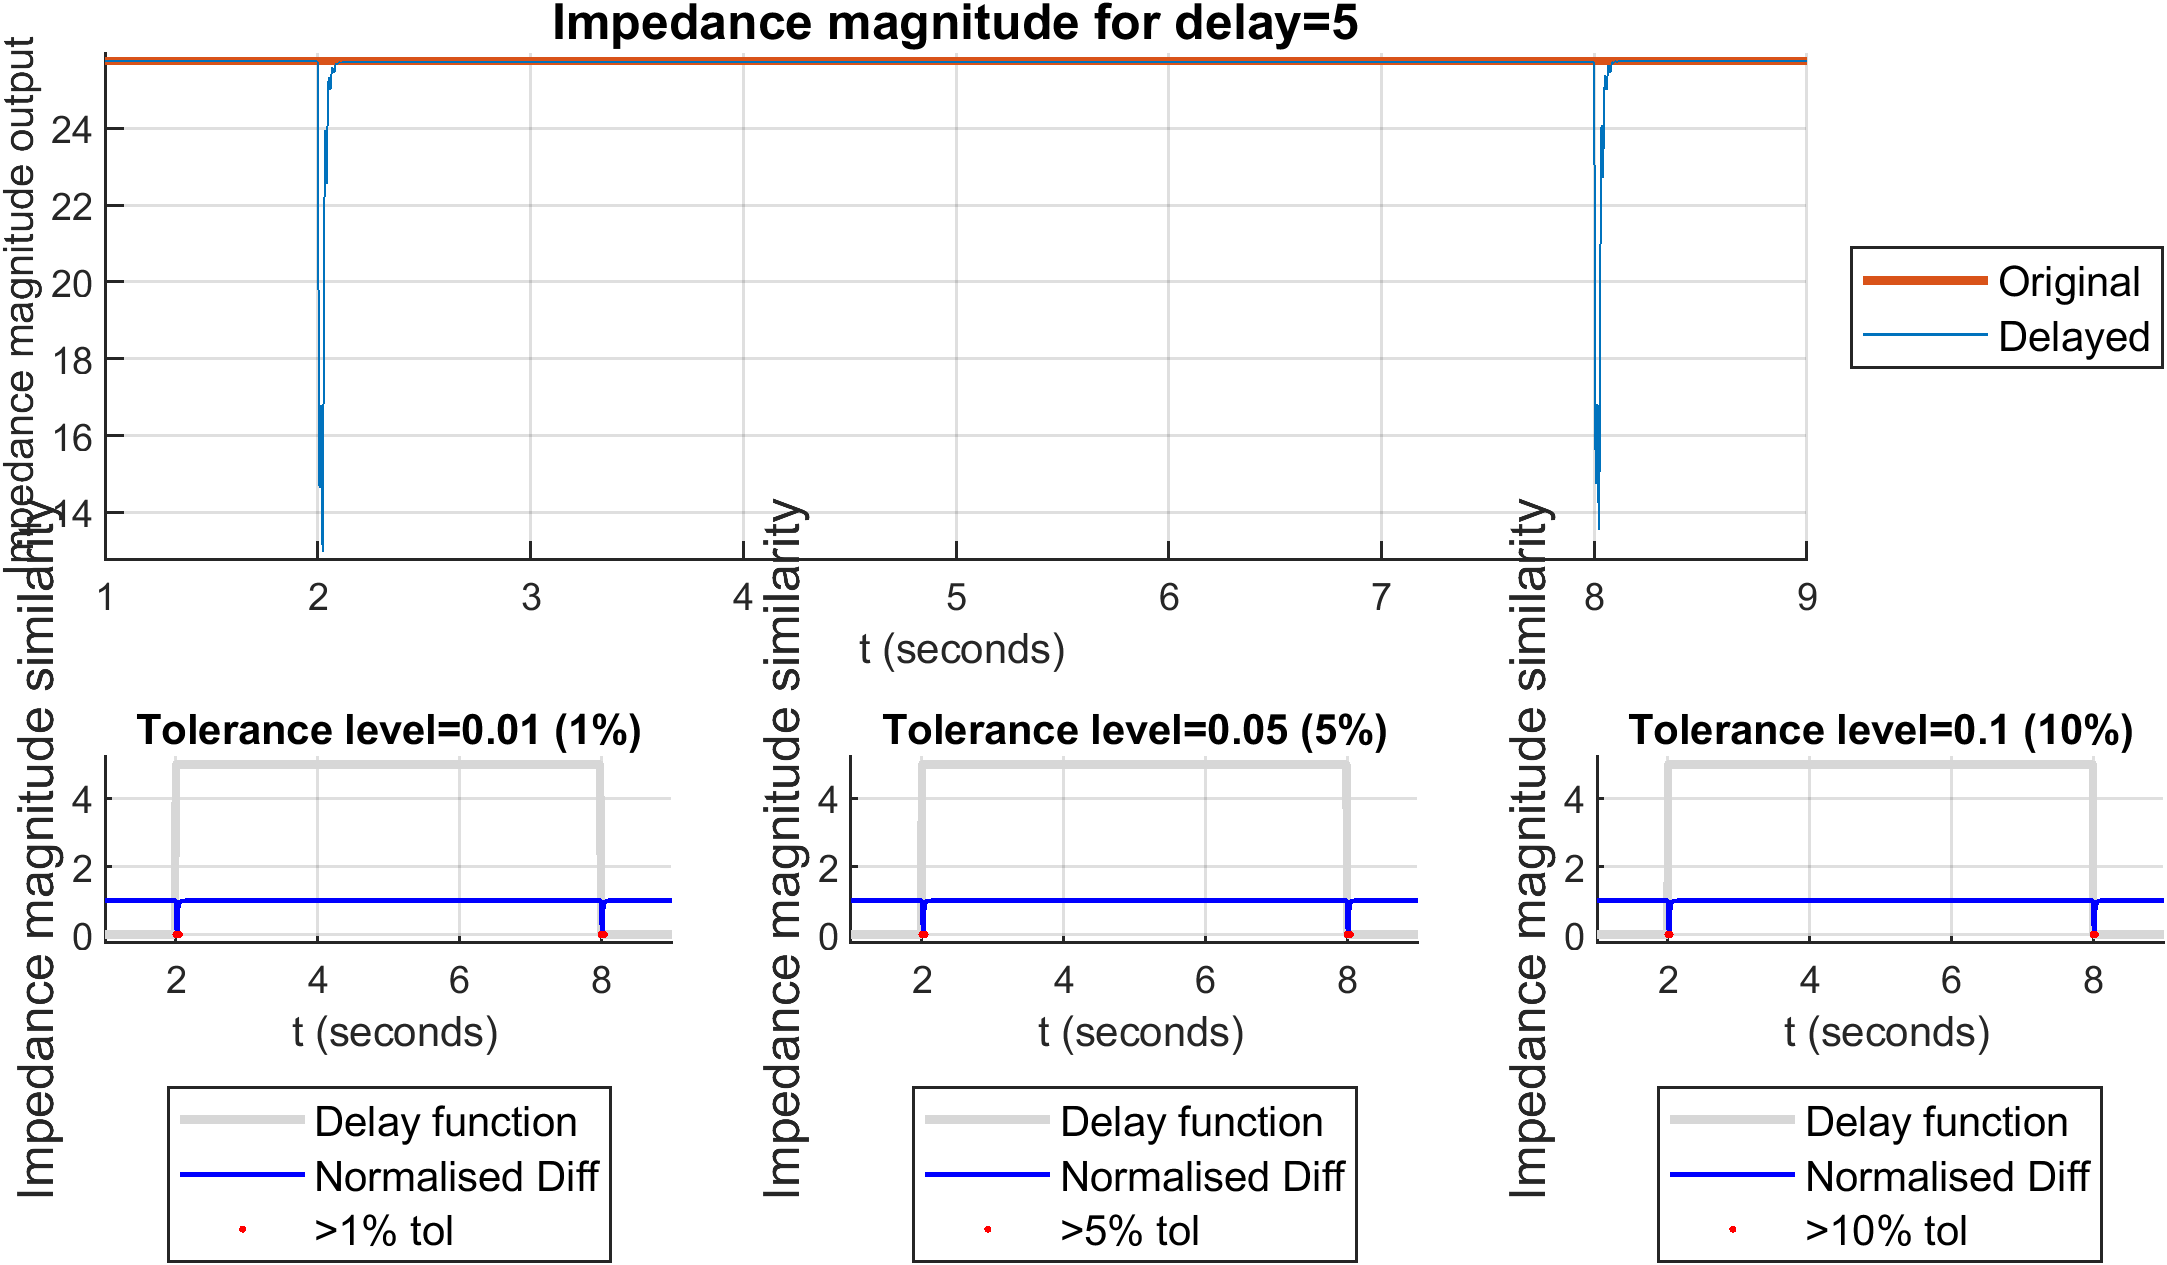
\includegraphics[width=0.95\textwidth]{PMUsim-figures/DelayOf_5/Instant_iMagnitude.png}}\\
 \label{fig:PMUsim_Five_Mag}
 %\caption{Instant Delay Magnitude Output for the Delay Level of Five}
  \end{tabular}
\caption[Instant delay of 5: Magnitude Output]{Results for Magnitude Output for Instant Delay equal to Five}
 \end{figure}
 
 
\newpage  
\begin{figure}[H]
\begin{tabular}{c}
   \fbox{     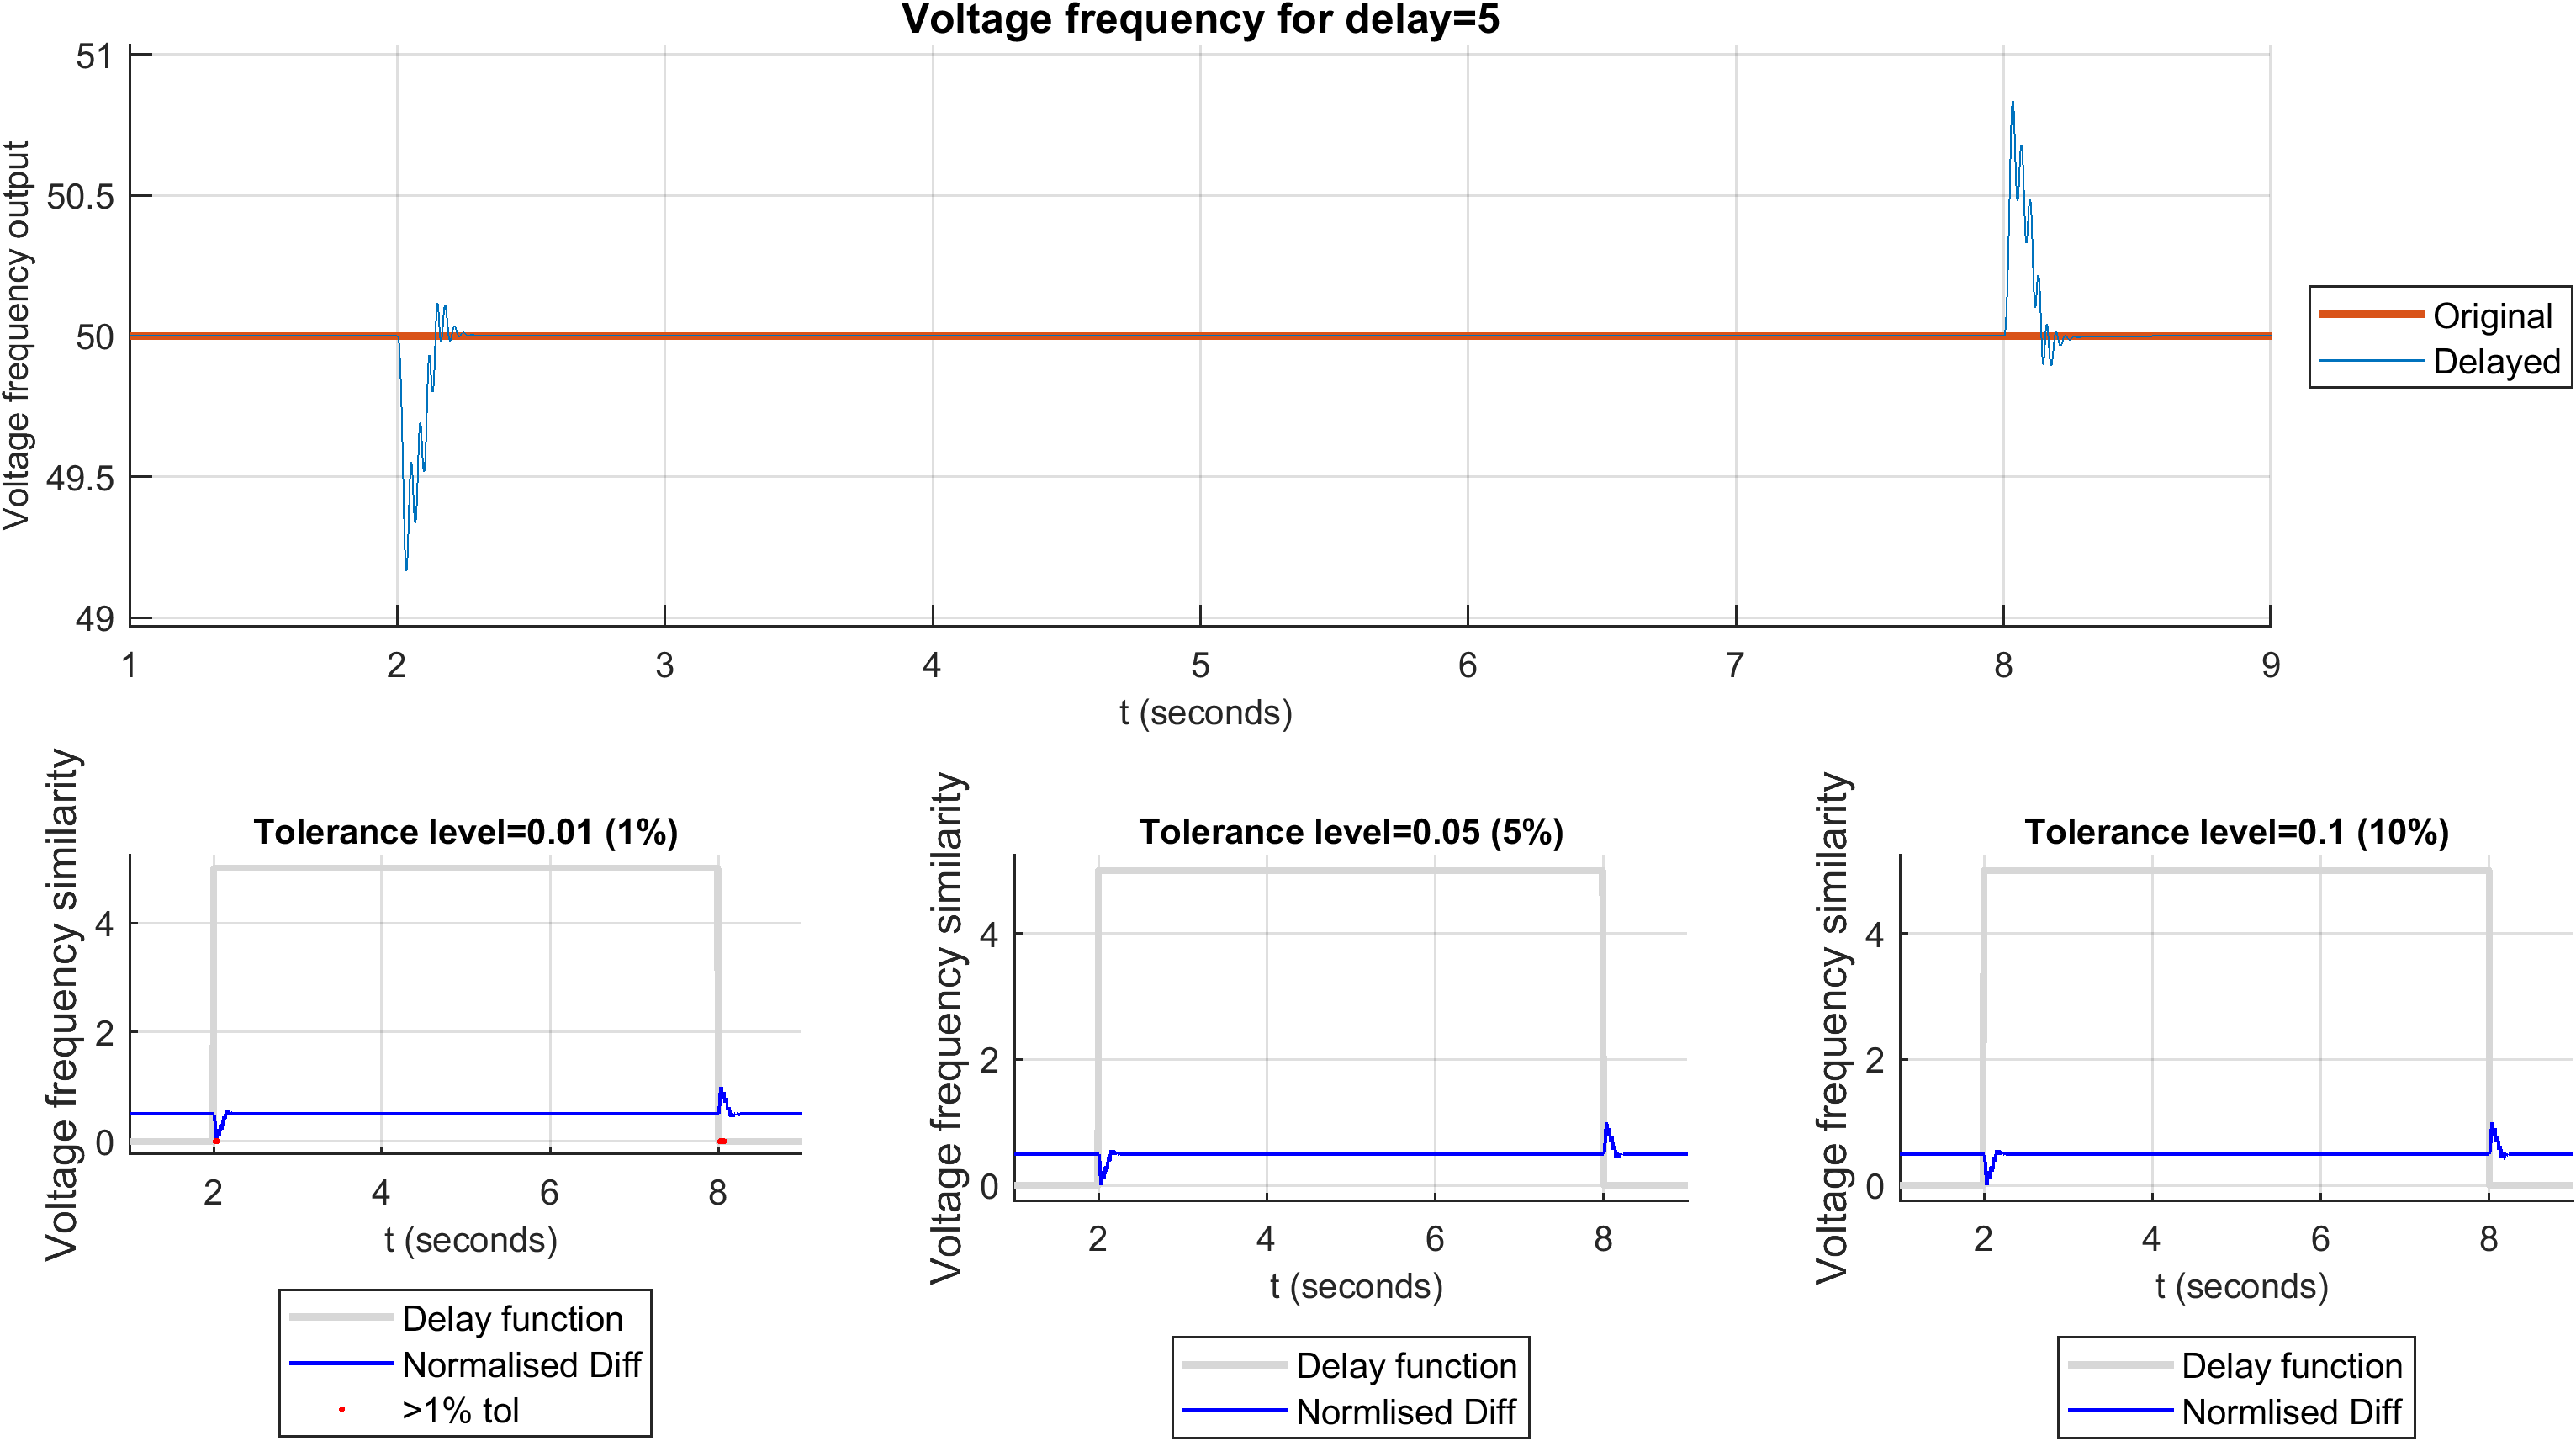
\includegraphics[width=0.95\textwidth]{PMUsim-figures/DelayOf_5/Instant_vFrequency.png}}\\
    \\ 
    
   \fbox{  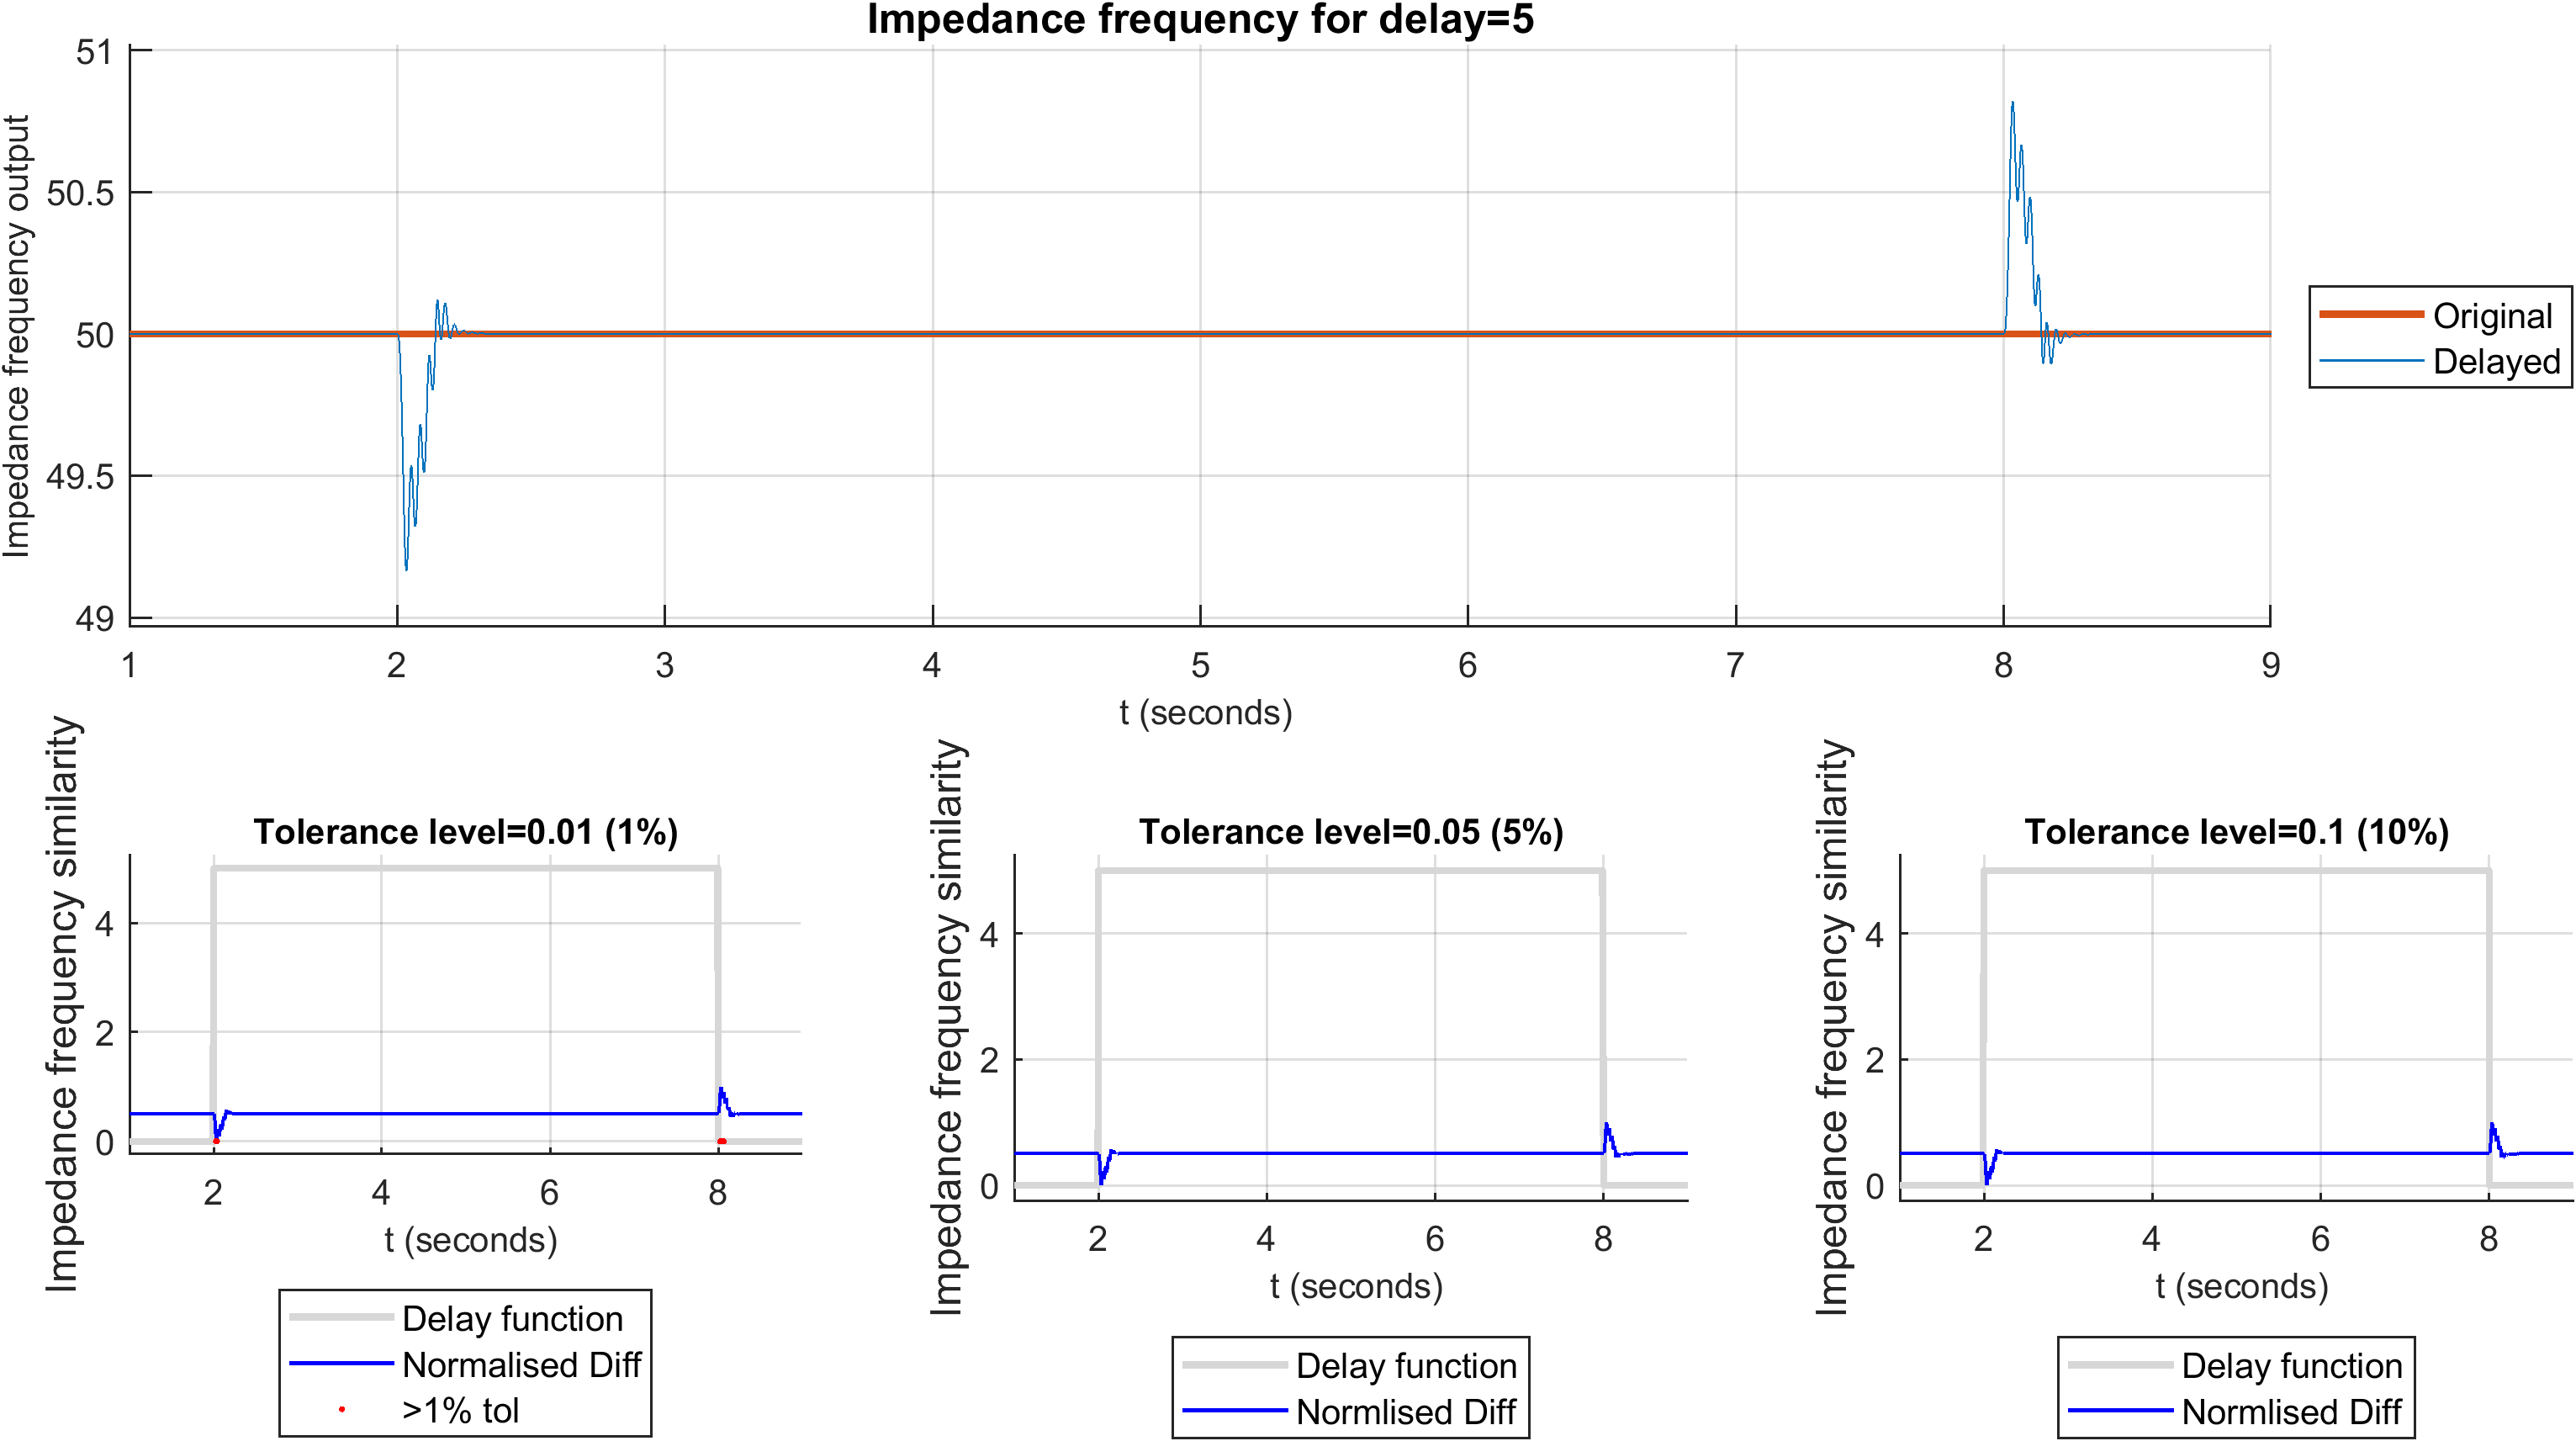
\includegraphics[width=0.95\textwidth]{PMUsim-figures/DelayOf_5/Instant_iFrequency.png}}\\
 \label{fig:PMUsim_Five_Freq}
 %\caption{Instant Delay Frequency Output for the Delay Level of Five}
  \end{tabular}
\caption[Instant delay of 5: Frequency Output]{Results for Frequency Output for Instant Delay equal to Five}
 \end{figure}
  

\newpage 
\begin{figure}[H]
\begin{tabular}{c}
   \fbox{     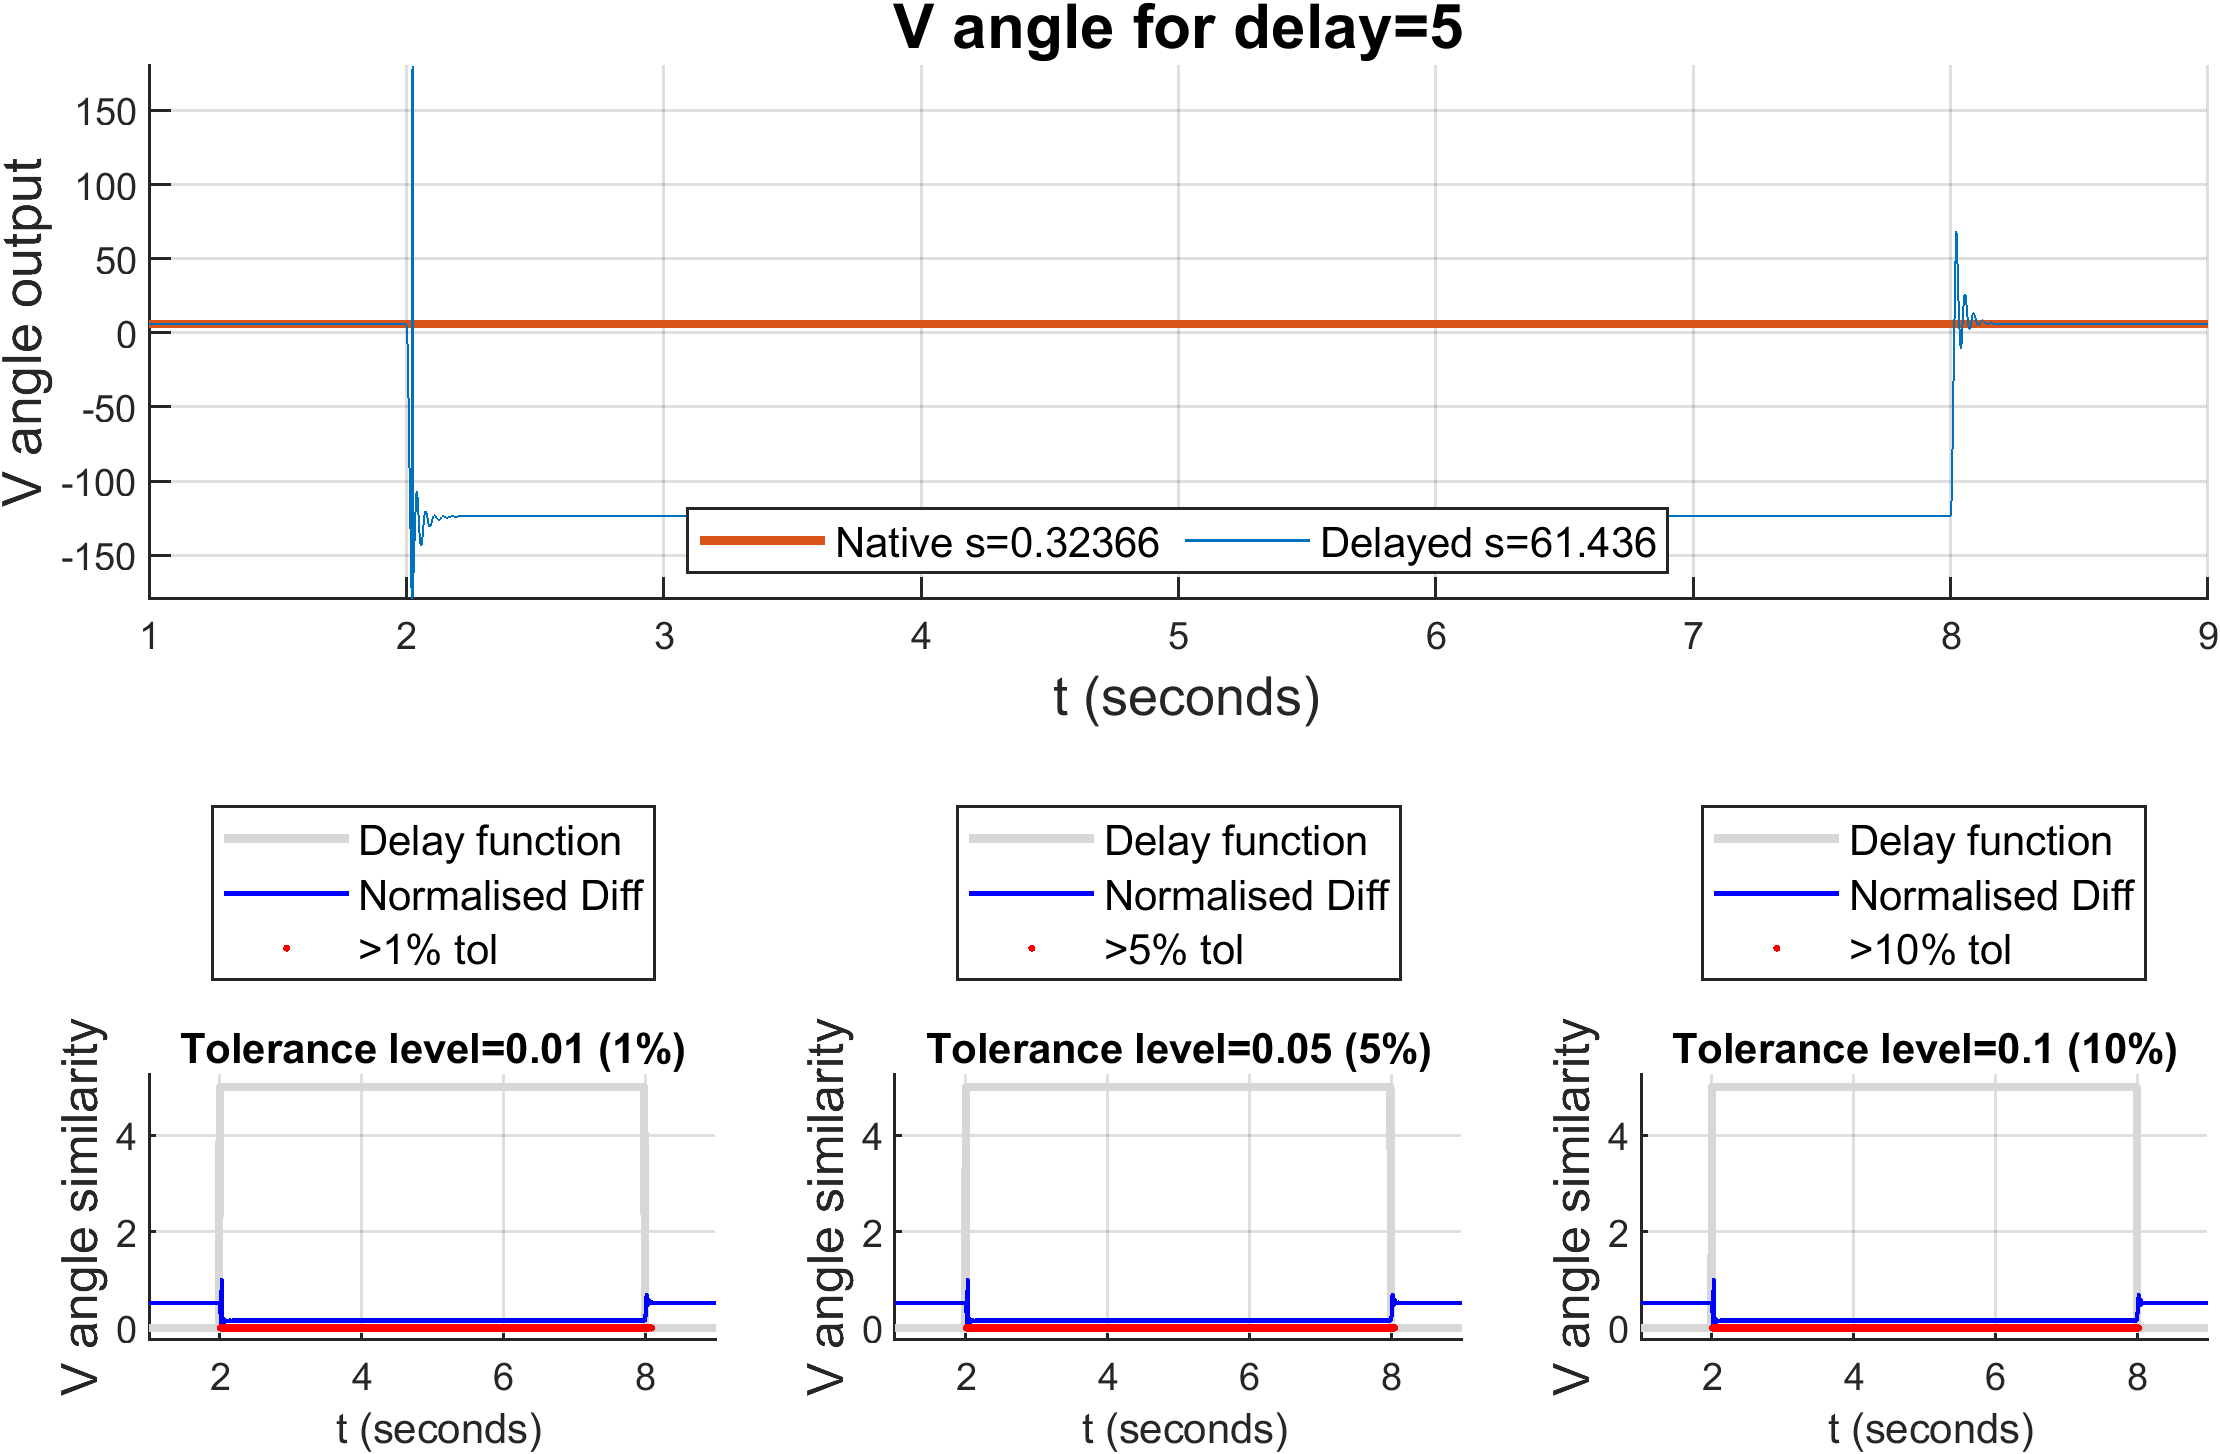
\includegraphics[width=0.95\textwidth]{PMUsim-figures/DelayOf_5/Instant_vAngle.png}}\\
    \\ 
    
   \fbox{  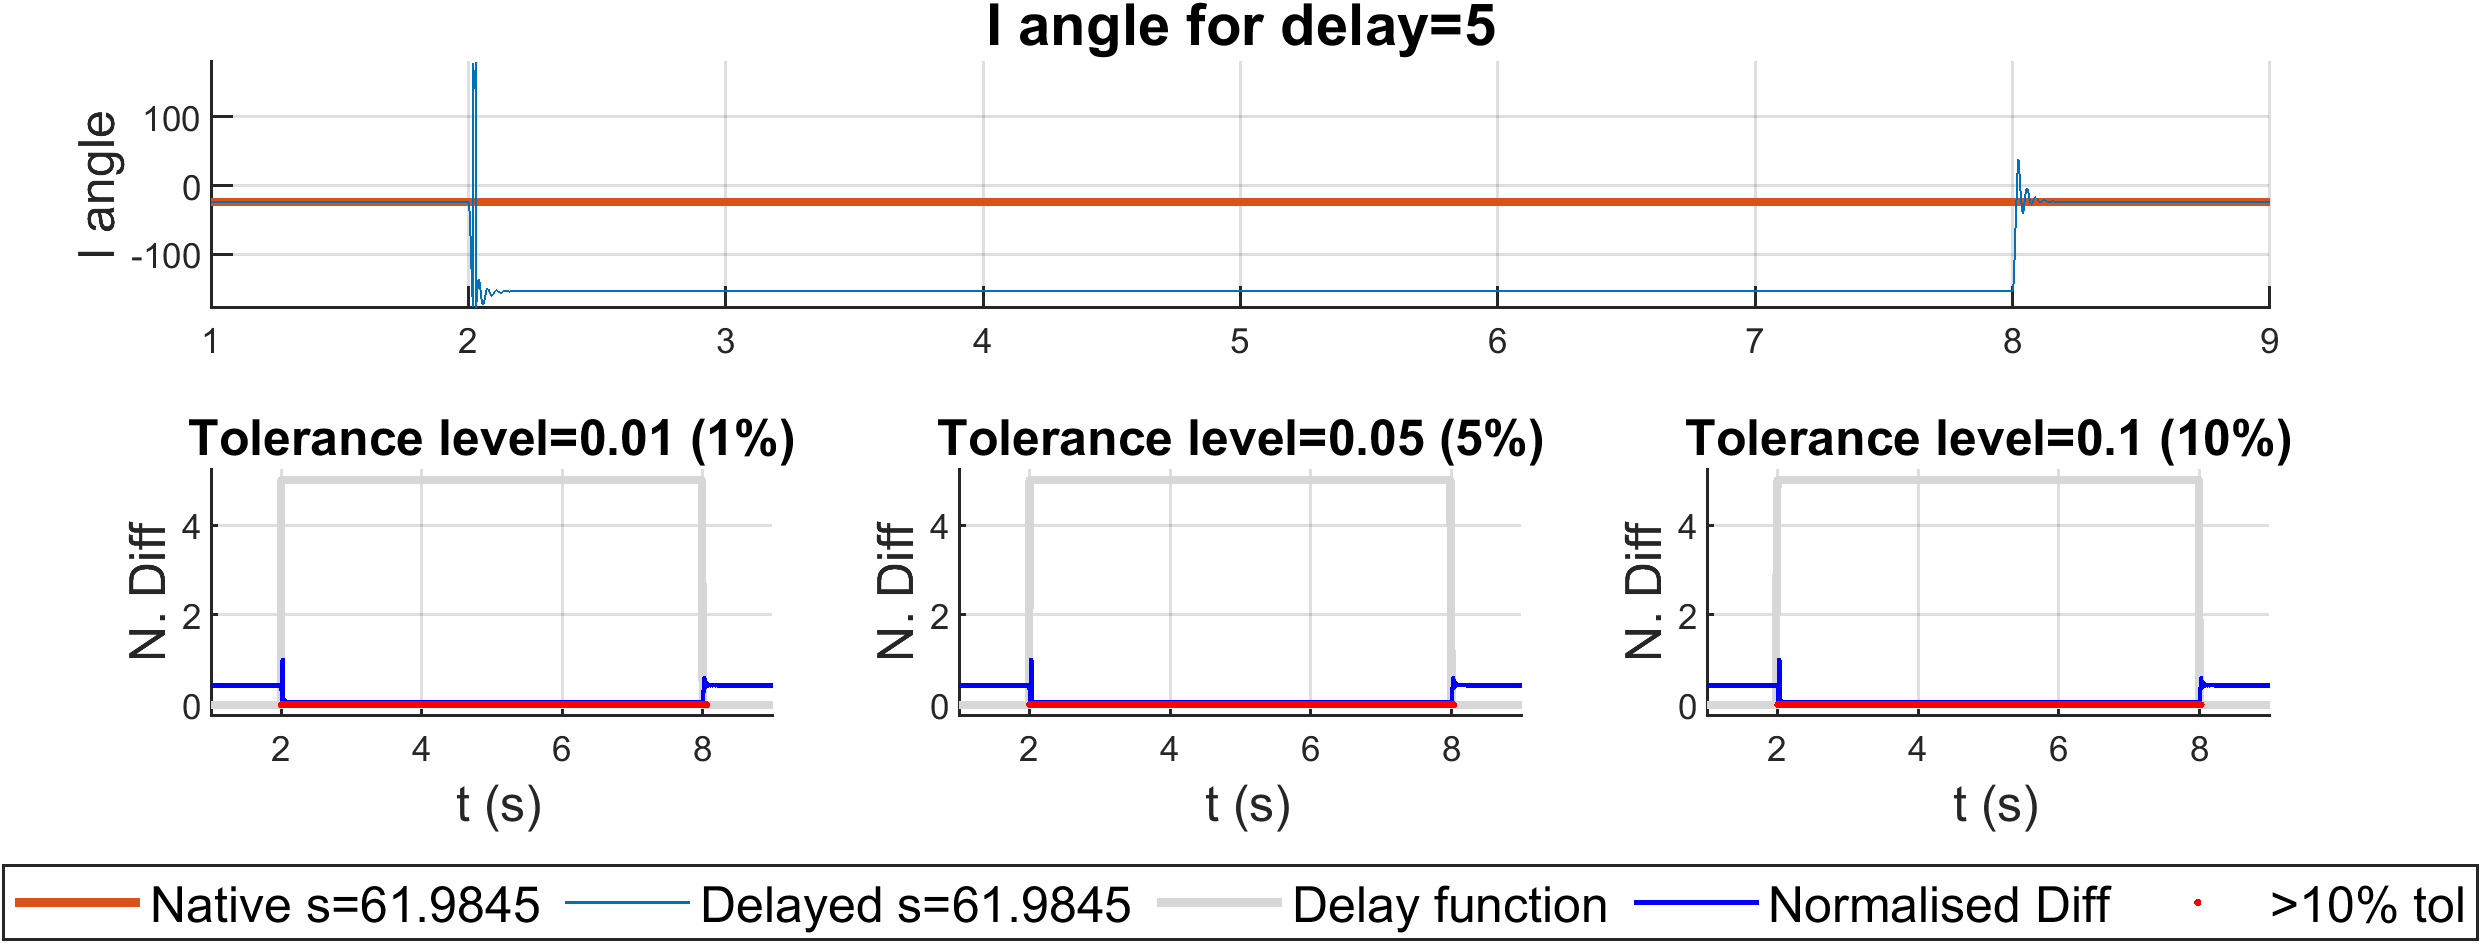
\includegraphics[width=0.95\textwidth]{PMUsim-figures/DelayOf_5/Instant_iAngle.png}}\\
 \label{fig:PMUsim_Five_Angle}
 %\caption{Instant Delay Angle Output for the Delay Level of Five}
  \end{tabular}
\caption[Instant delay of 5: Angle Output]{Results for Angle Output for Instant Delay equal to Five}
 \end{figure}
 

\newpage 
\subsection{Instant Delay Level of Six}


\begin{small}
     \tcbox[size=normal, standard jigsaw, opacityback=0, boxrule=0pt,halign=justify]{
     Instant Delay Level of Six}{
          \begin{itemize}
         \item      The delayed signal (blue) overlaps the original signal (red), producing a straight line, colored neither red nor blue.
         \item  The blue Normalised diff signal also overlaps the grey delay function.
          \end{itemize} }
\end{small}


\newpage 
\begin{figure}[H]
\begin{tabular}{c}
   \fbox{    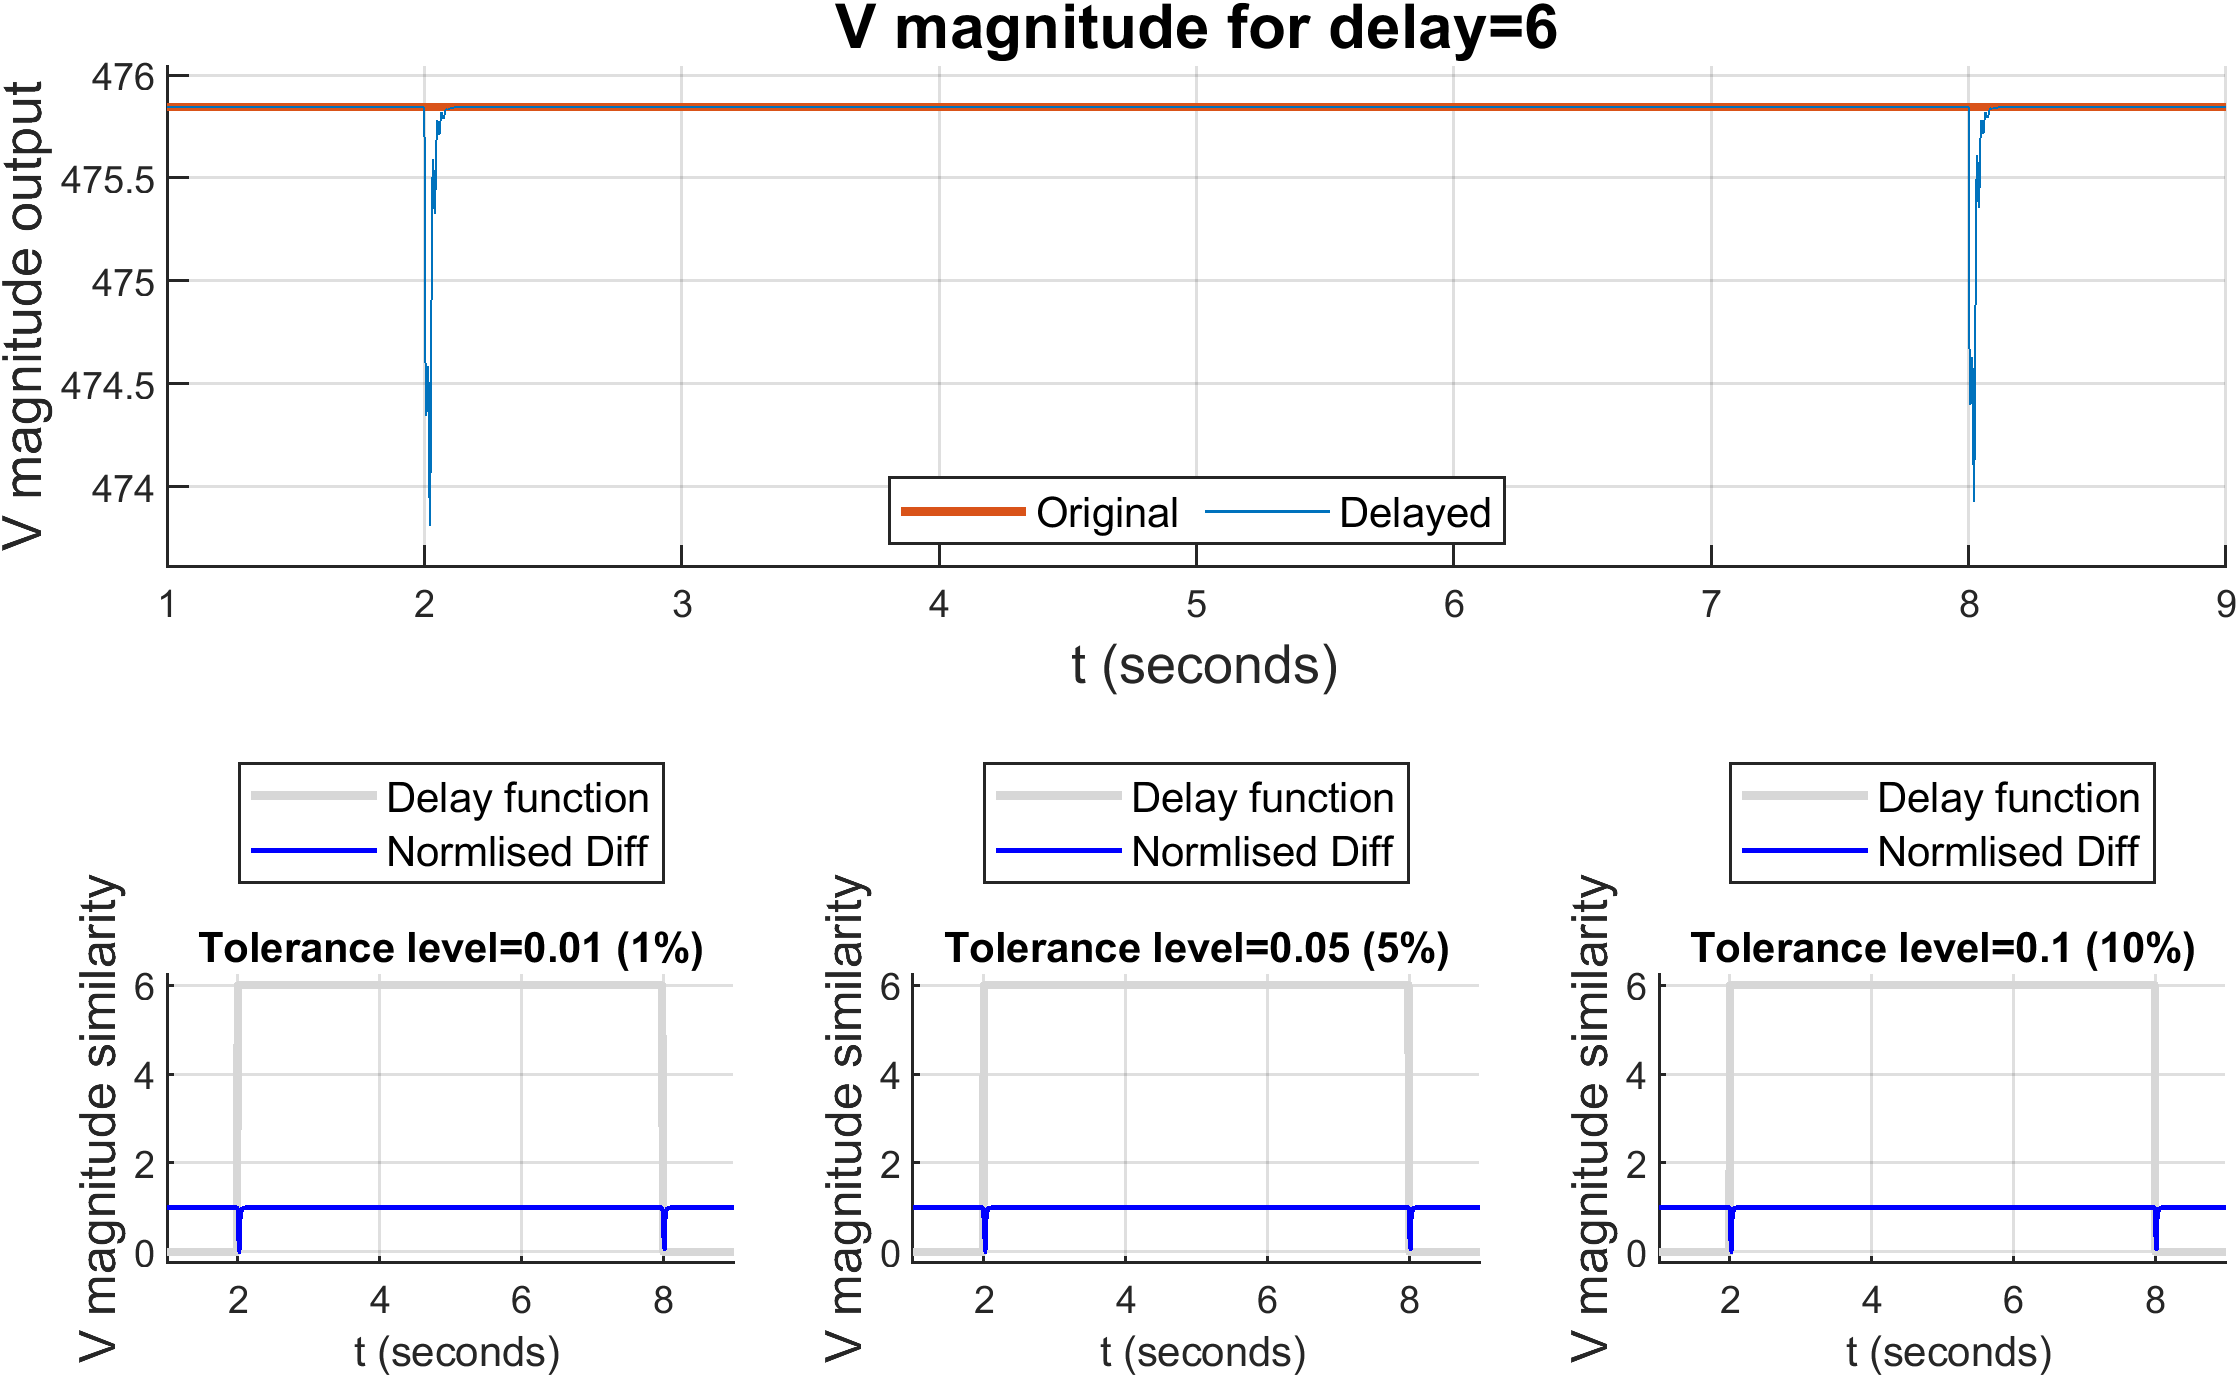
\includegraphics[width=0.95\textwidth]{PMUsim-figures/DelayOf_6/Instant_vMagnitude.png}}\\
  
      \\ 
   \fbox{    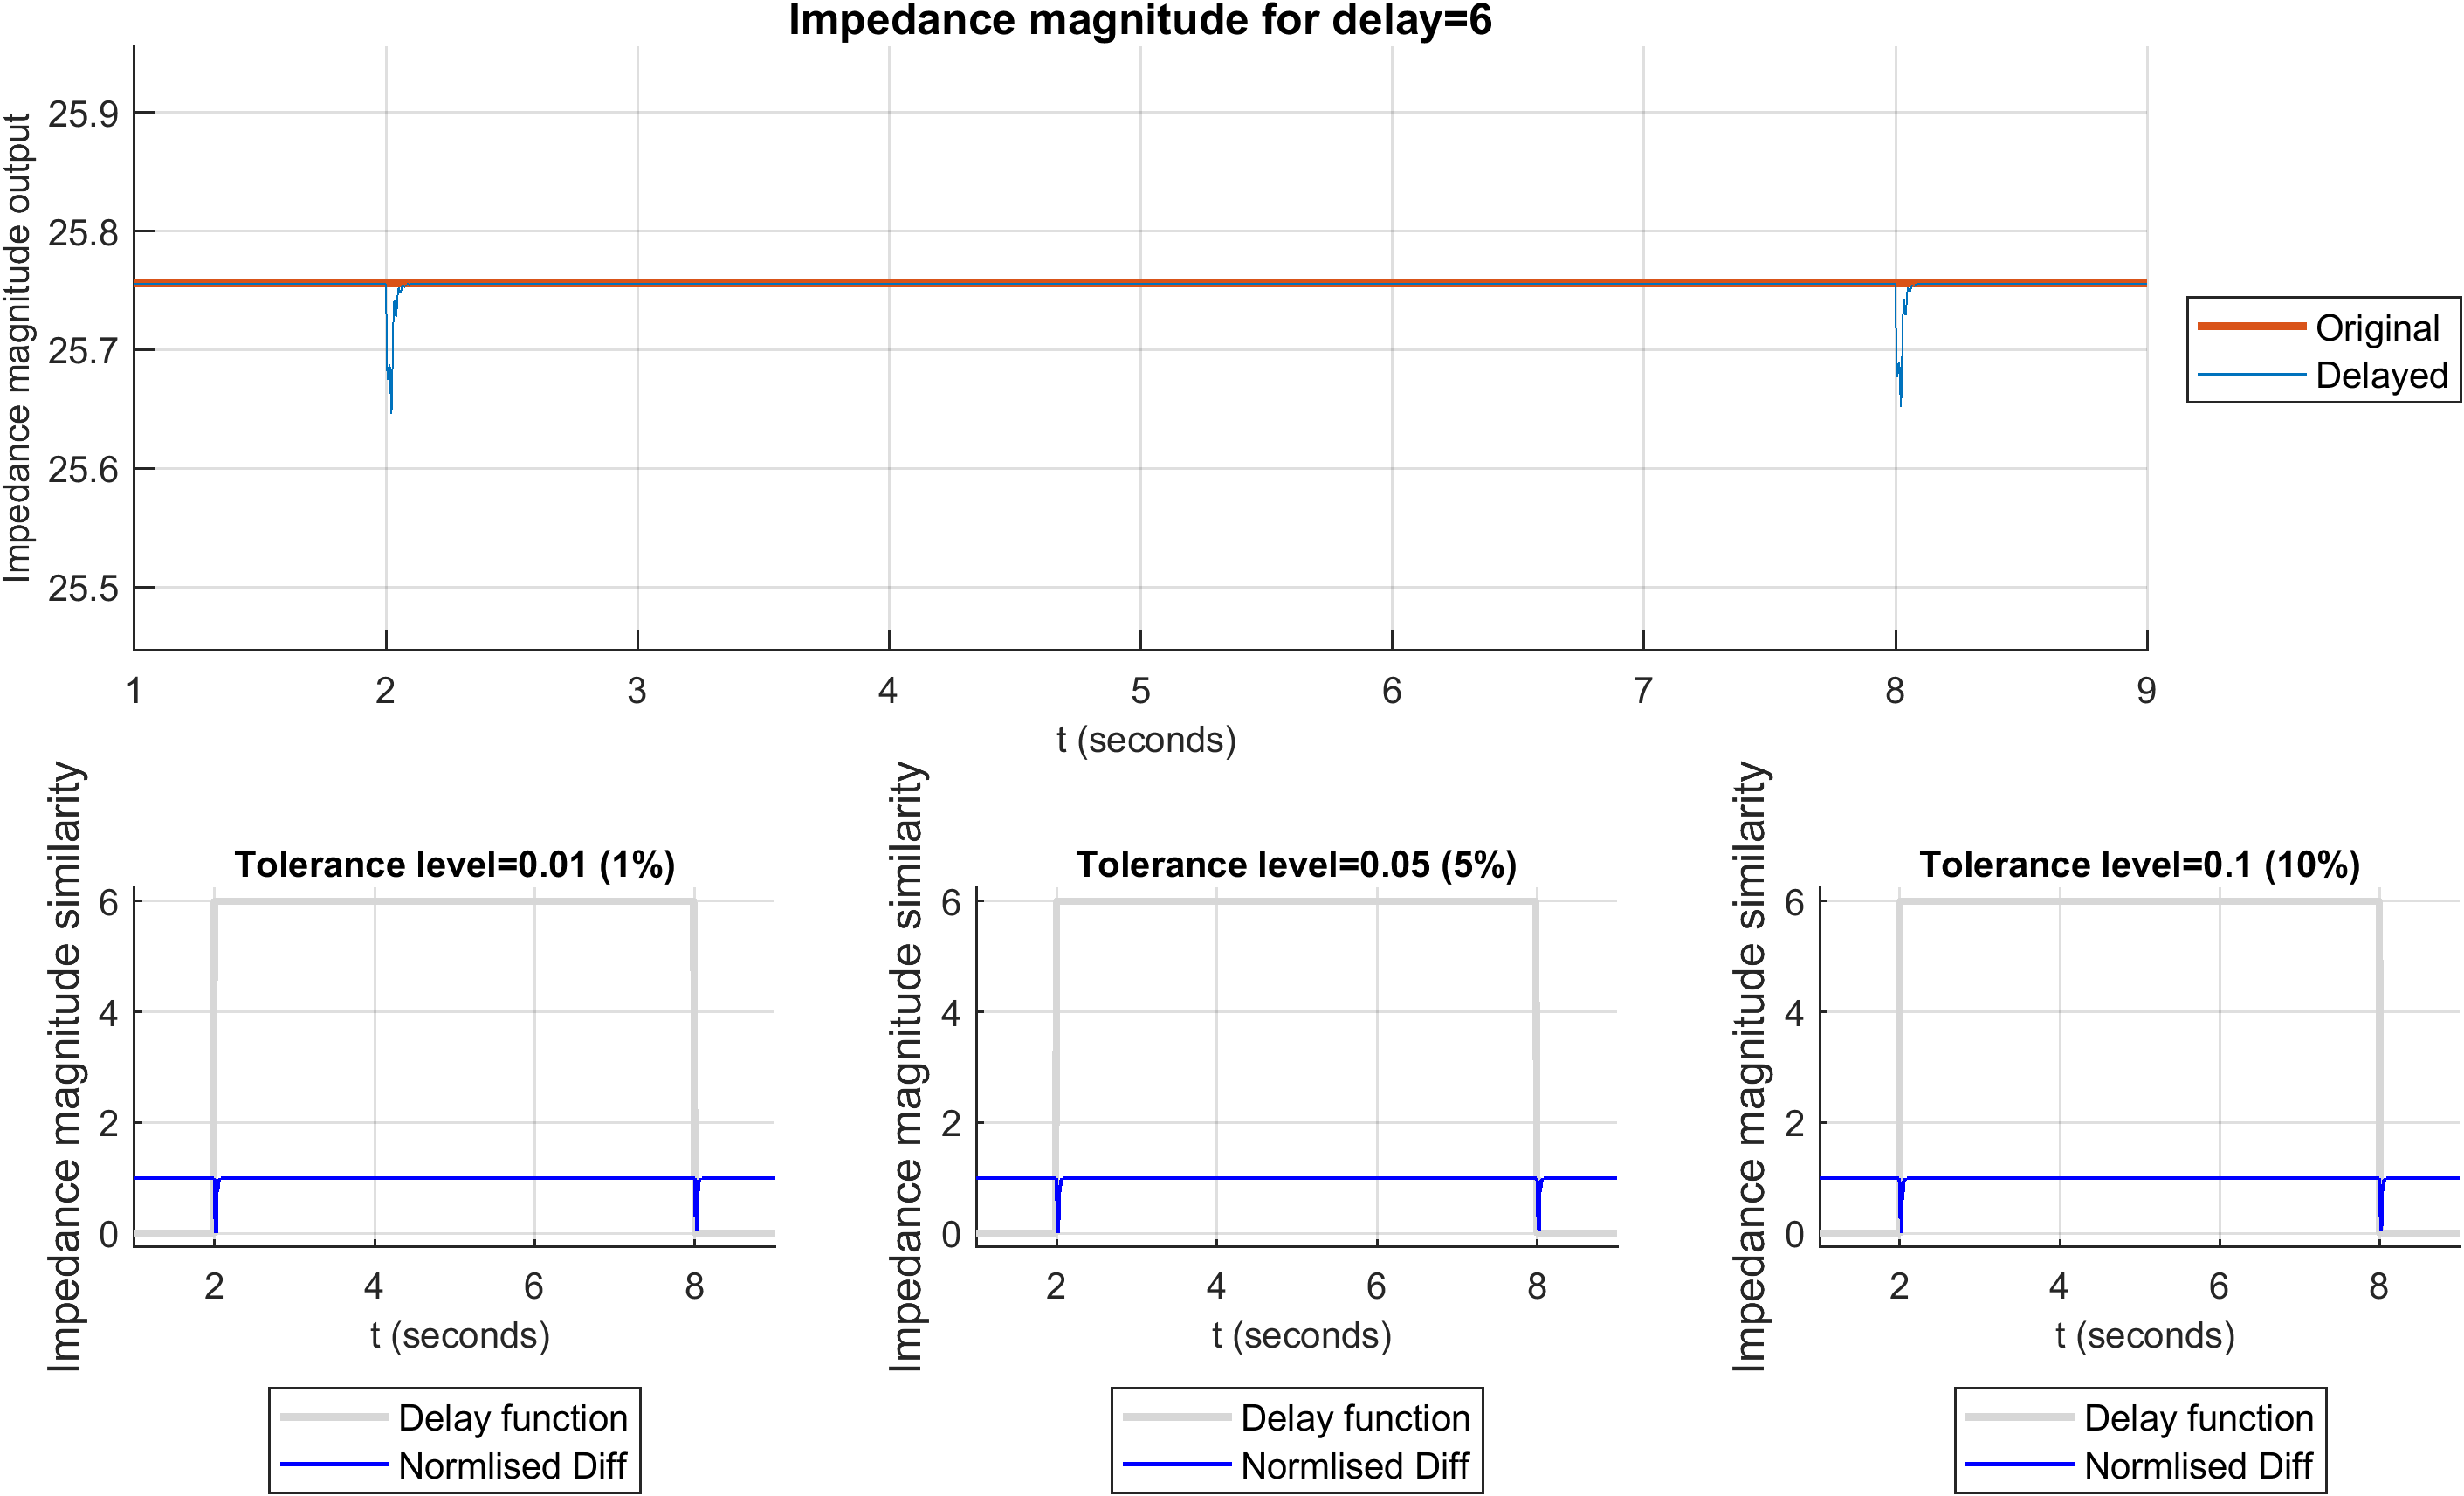
\includegraphics[width=0.95\textwidth]{PMUsim-figures/DelayOf_6/Instant_iMagnitude.png}}\\  
 \label{fig:PMUsim_Six_Mag}
 %\caption{Instant Delay Magnitude Output for the Delay Level of Six}
  \end{tabular}
\caption[Instant delay of 6: Magnitude Output]{Results for Magnitude Output for Instant Delay equal to Six}
 \end{figure}

\newpage  
\begin{figure}[H]
\begin{tabular}{c}
   \fbox{     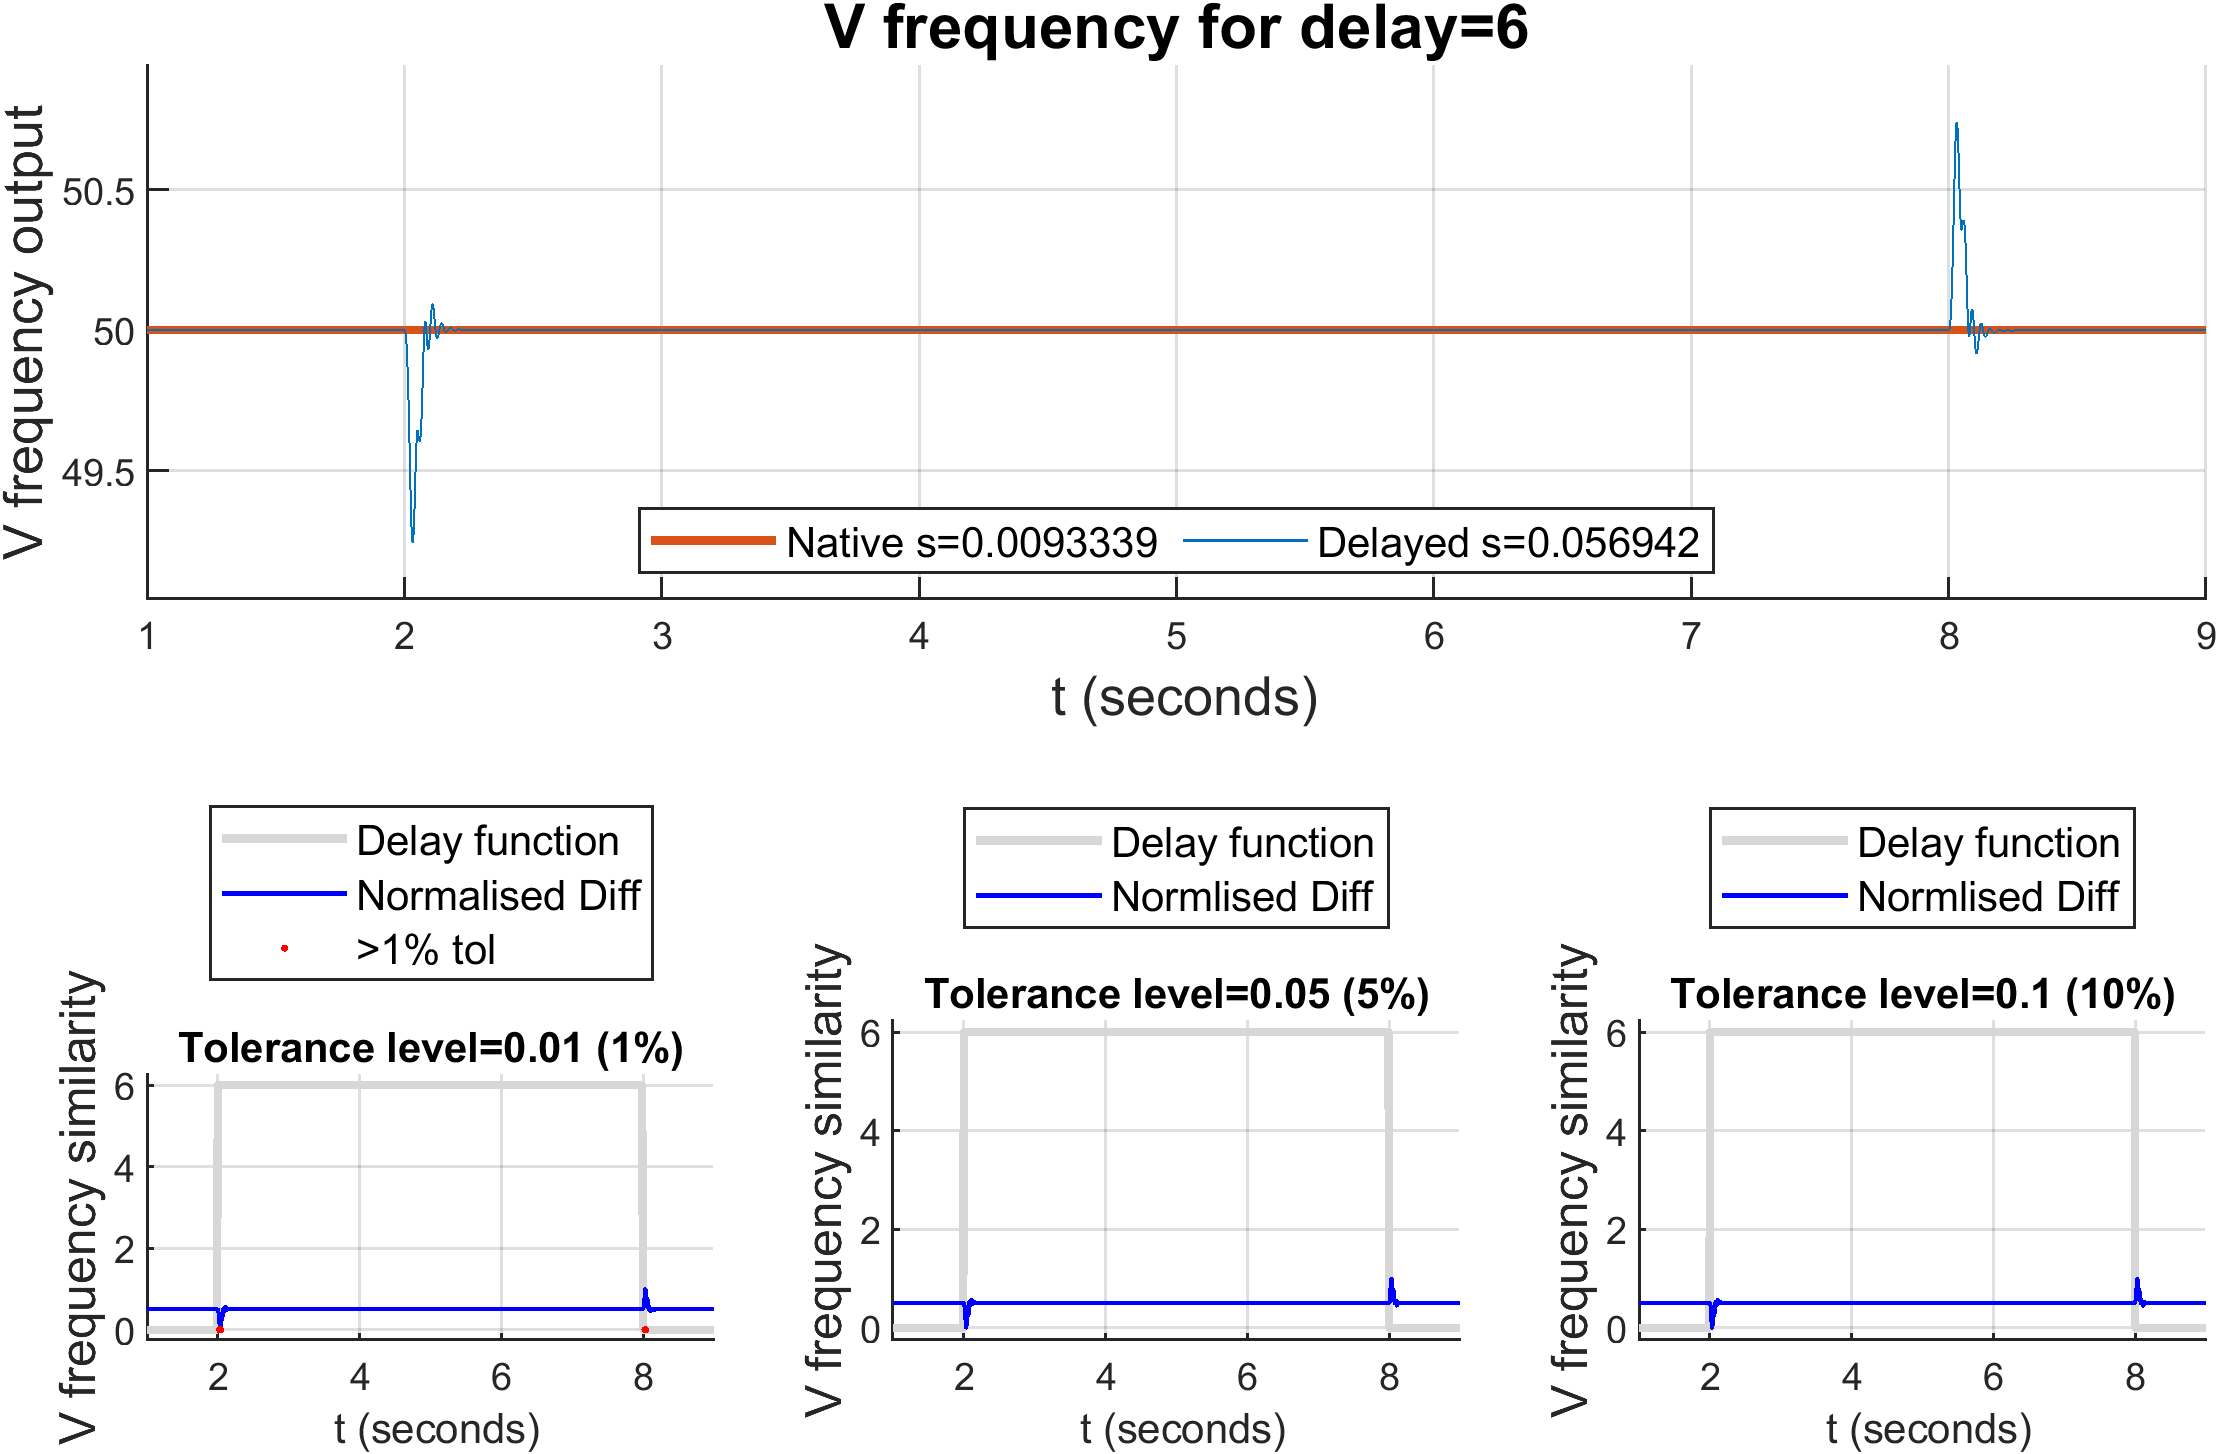
\includegraphics[width=0.95\textwidth]{PMUsim-figures/DelayOf_6/Instant_vFrequency.png}}\\
  
      \\ 
   \fbox{  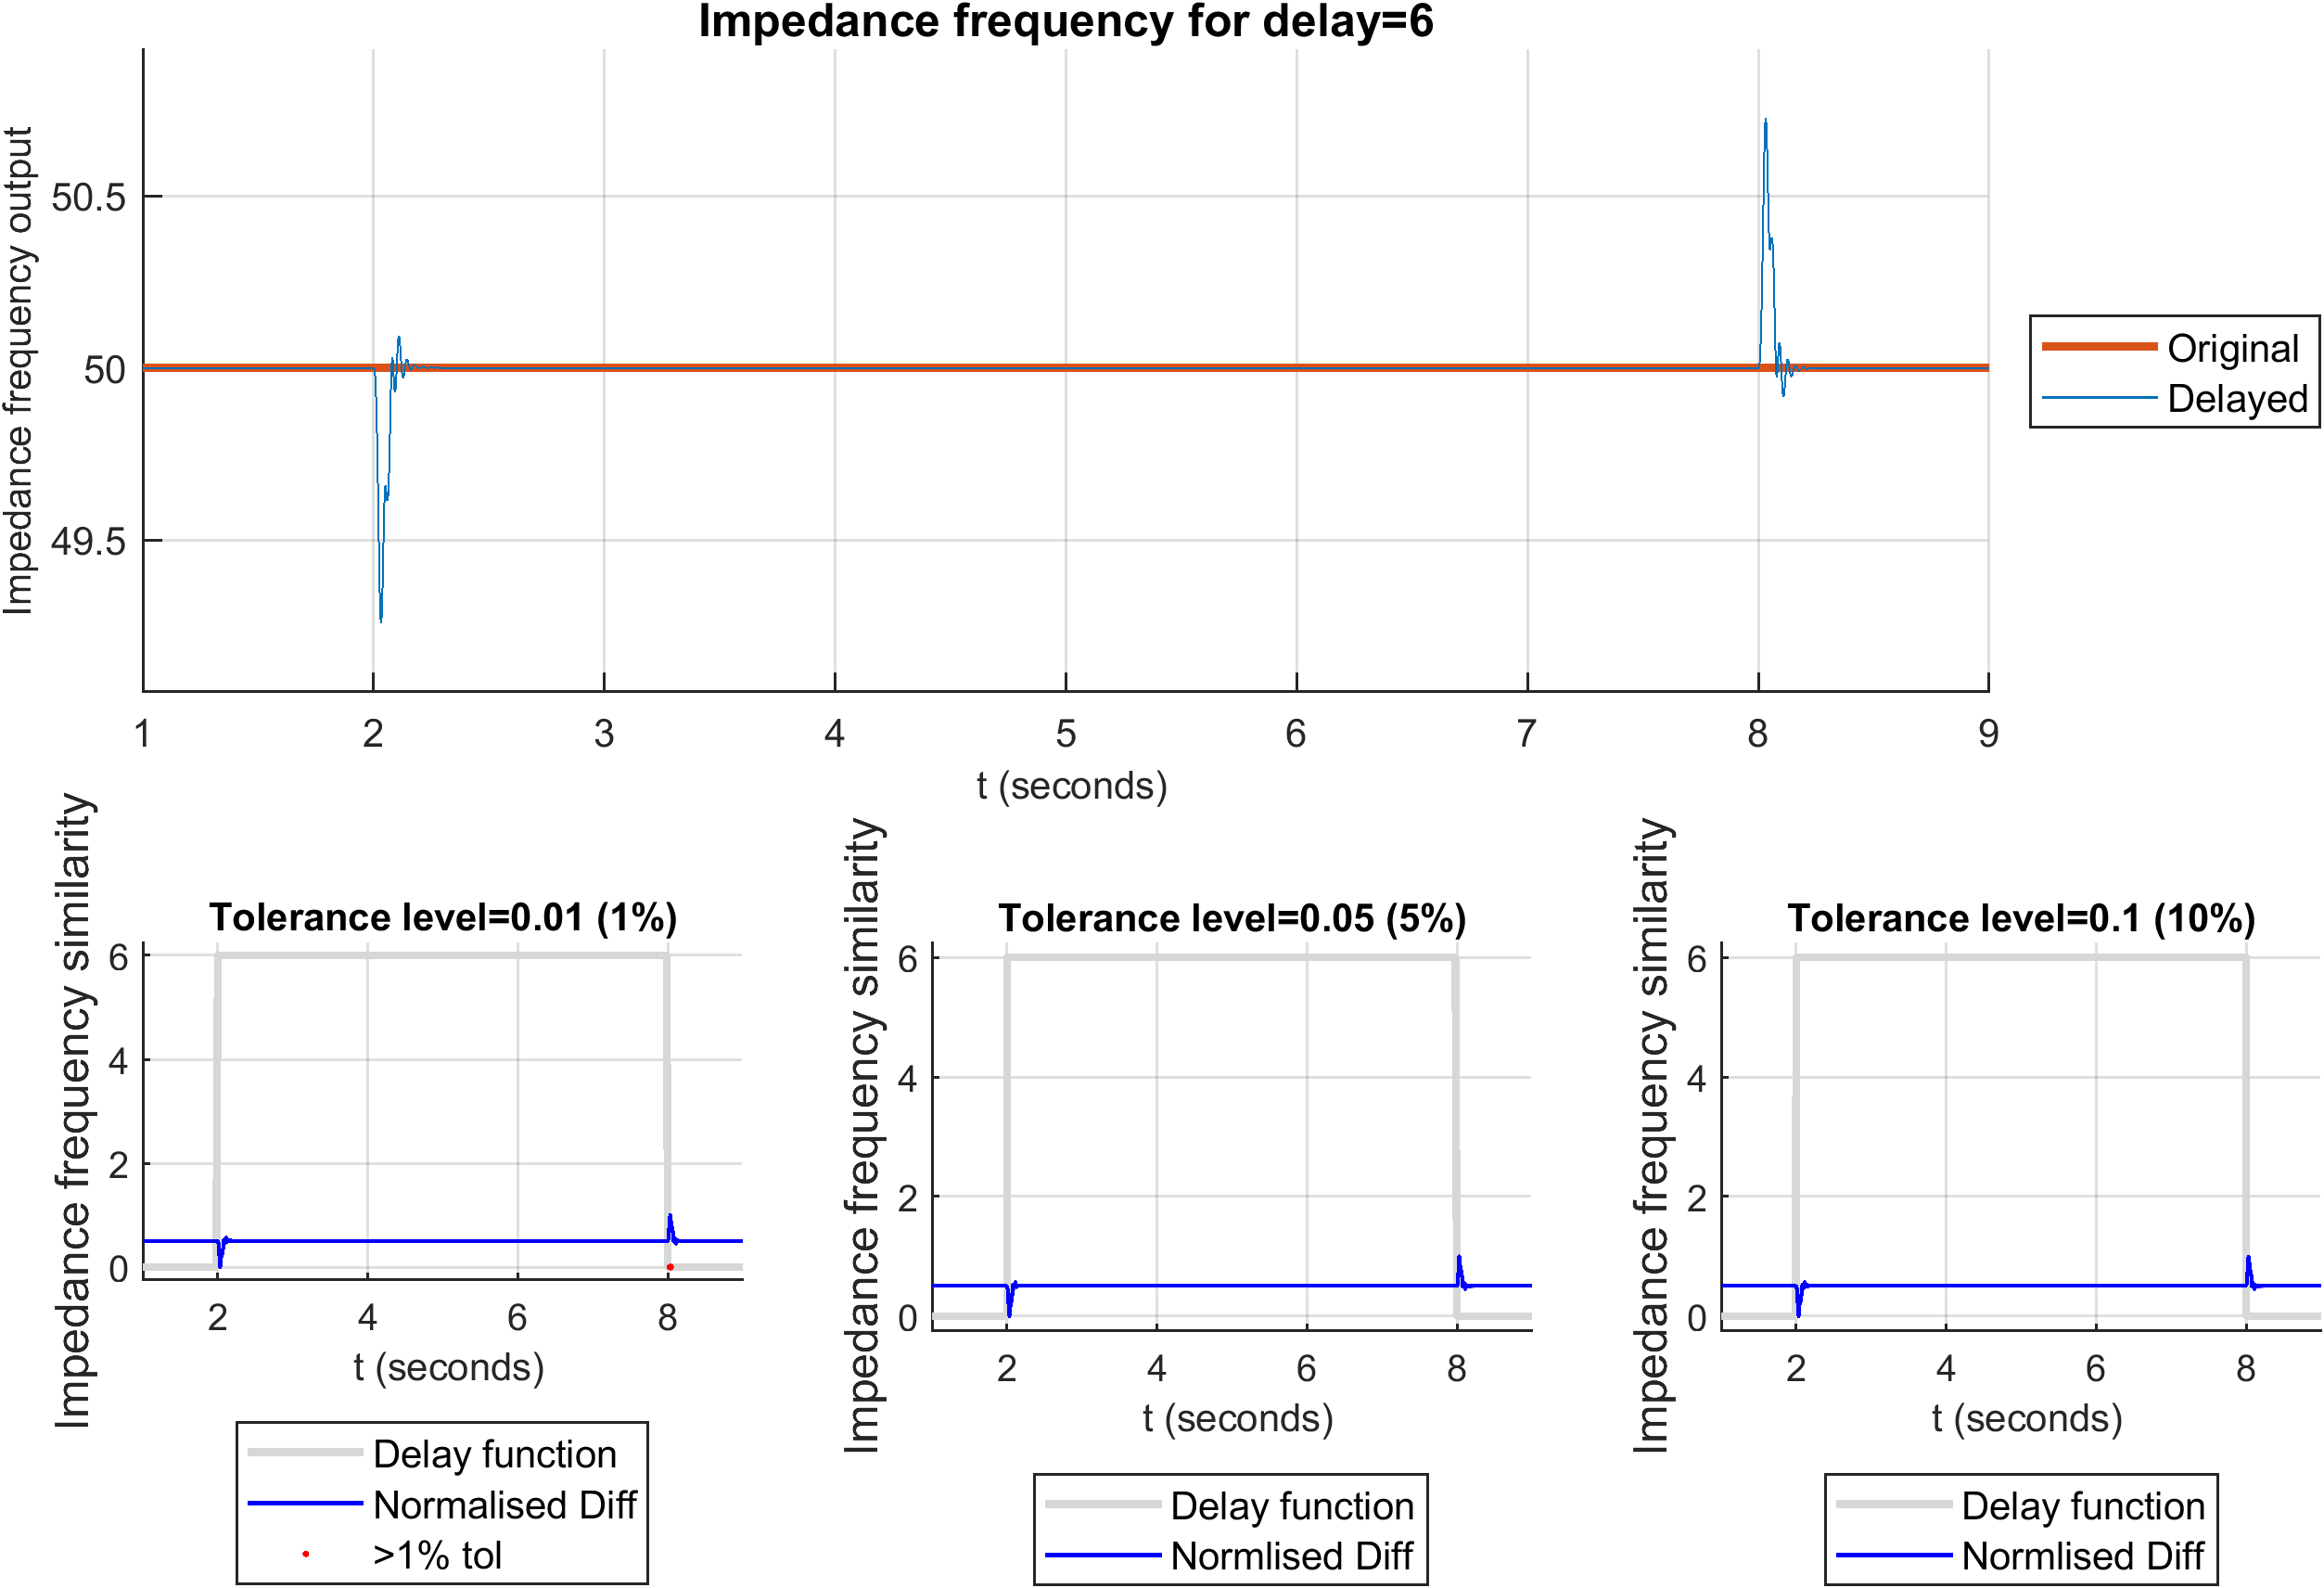
\includegraphics[width=0.95\textwidth]{PMUsim-figures/DelayOf_6/Instant_iFrequency.png}}\\ 
 \label{fig:PMUsim_Six_Freq}
 %\caption{Instant Delay Frequency Output for the Delay Level of Six}
  \end{tabular}
\caption[Instant delay of 6: Frequency Output]{Results for Frequency Output for Instant Delay equal to Six}
 \end{figure}
   


\newpage 
\begin{figure}[H]
\begin{tabular}{c}
   \fbox{     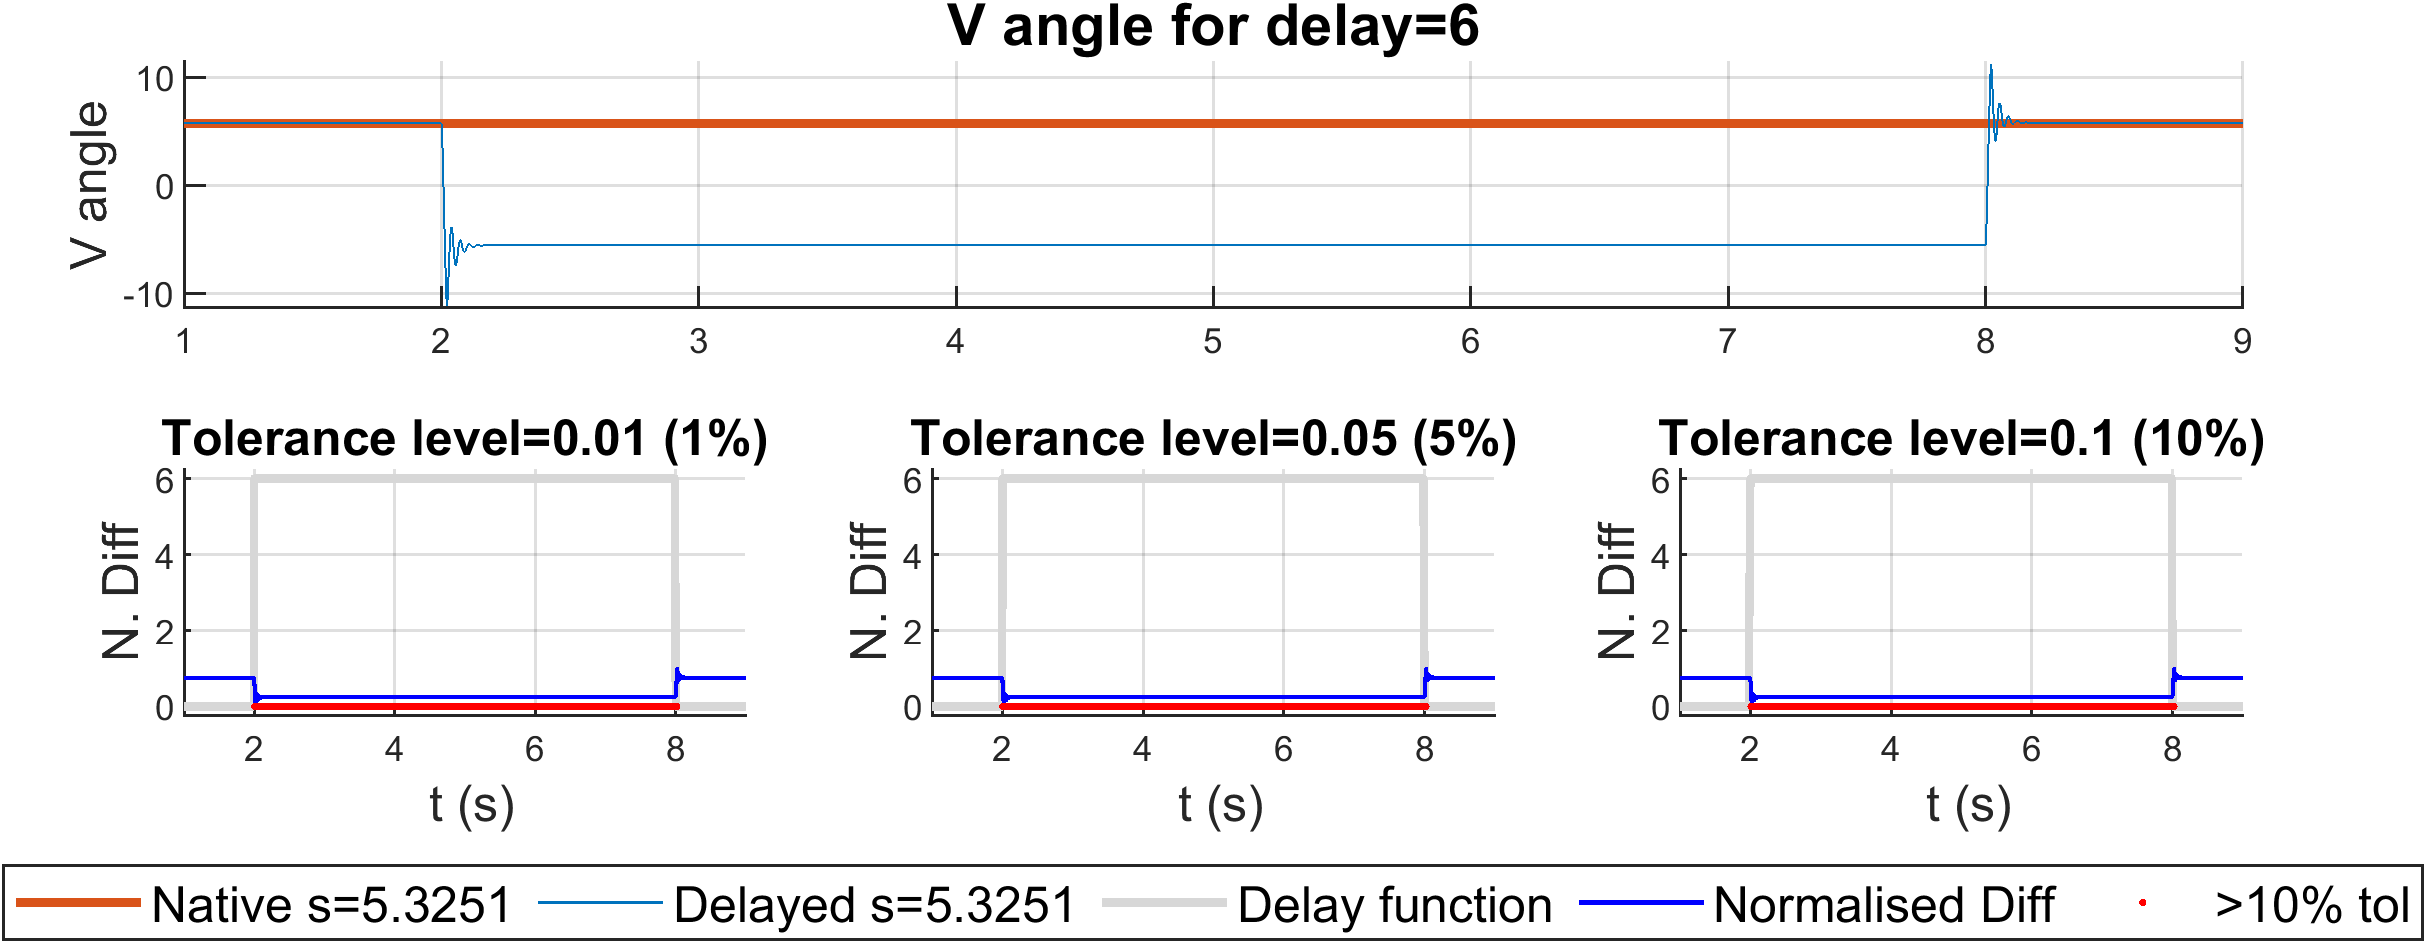
\includegraphics[width=0.95\textwidth]{PMUsim-figures/DelayOf_6/Instant_vAngle.png}}\\
      \\ 
    
   \fbox{  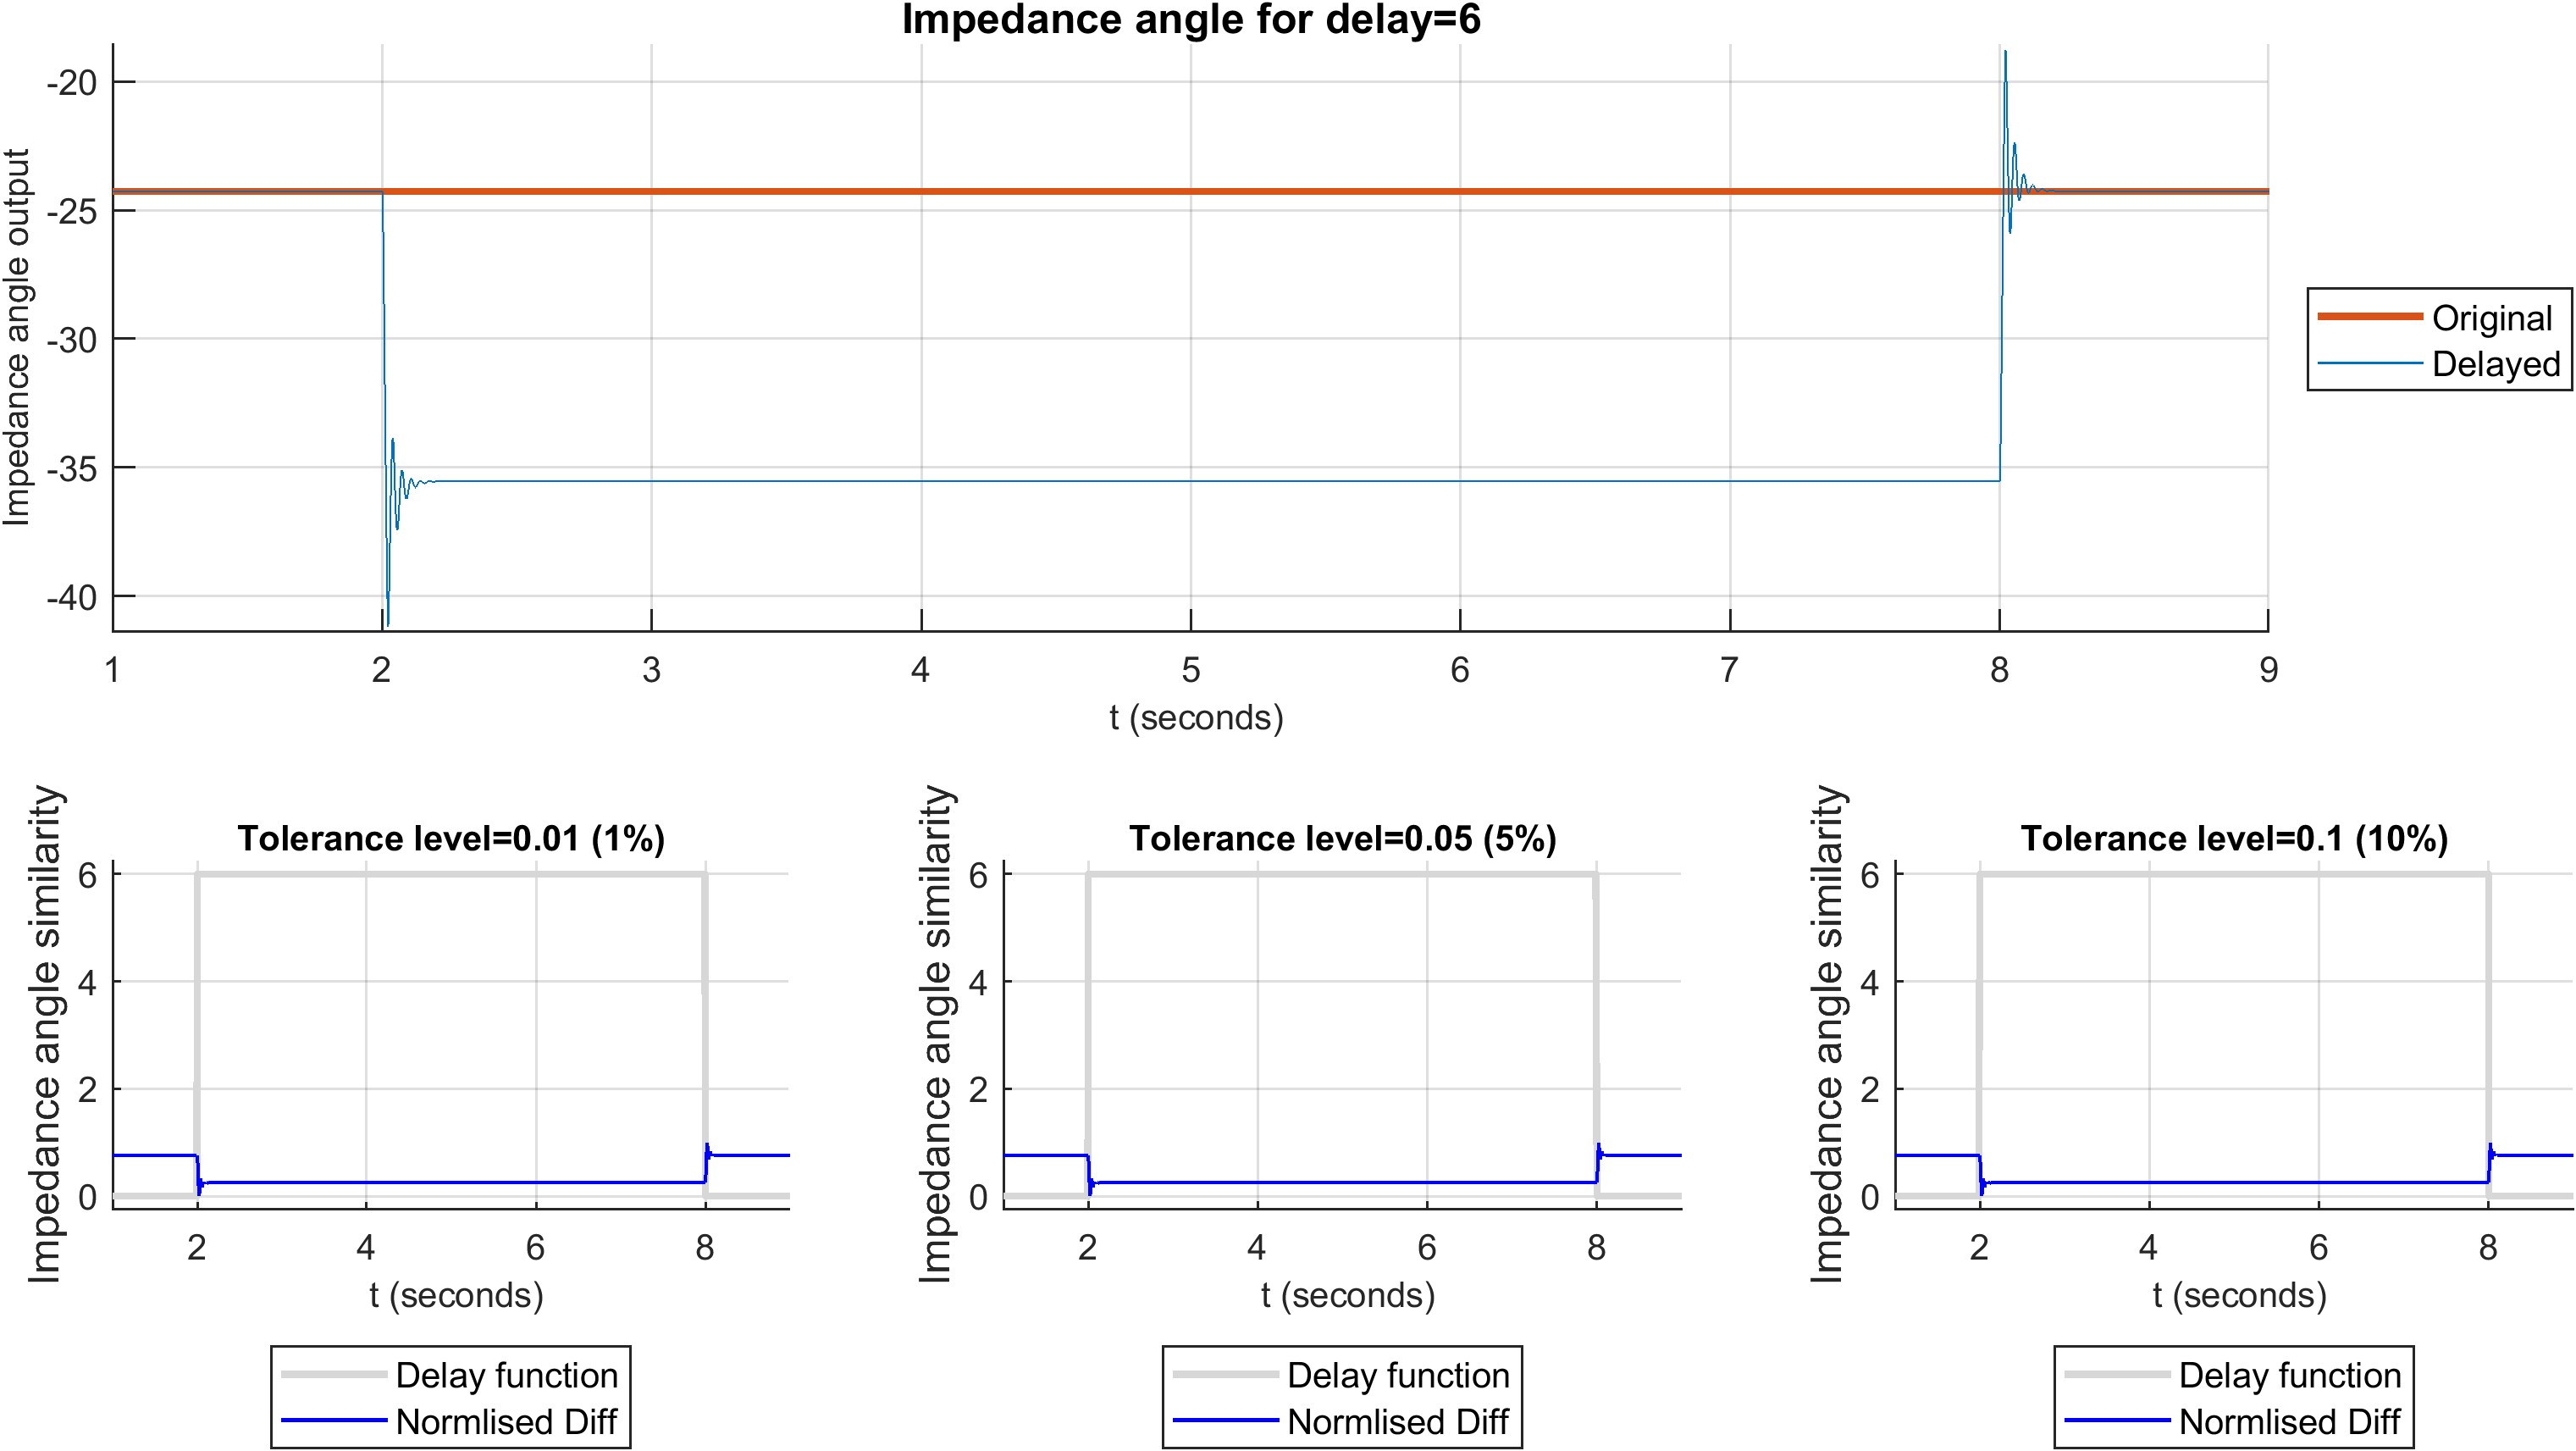
\includegraphics[width=0.95\textwidth]{PMUsim-figures/DelayOf_6/Instant_iAngle.png}}\\
 \label{fig:PMUsim_Six_Angle}
 %\caption{Instant Delay Angle Output for the Delay Level of Six}
  \end{tabular}
\caption[Instant delay of 6: Angle Output]{Results for Angle Output for Instant Delay equal to Six}
 \end{figure}
 
\newpage 
\section{Step-Wise Delay Functions}

\begin{small}
     \tcbox[size=normal, standard jigsaw, opacityback=0, boxrule=0pt,halign=justify]{
     Step-Wise Delay Functions}{
          \begin{itemize}
         \item      The delayed signal (blue) overlaps the original signal (red), producing a straight line, colored neither red nor blue.
         \item  The blue Normalised diff signal also overlaps the grey delay function.
          \end{itemize} }
\end{small}


\subsection{Step-Wise Delay Level of Two}
\newpage 

 \begin{small}
    \tcbox[size=normal, standard jigsaw, opacityback=0, boxrule=0pt,halign=justify]{
     Step-Wise Delay Level of Two}{
          \begin{itemize}
         \item      The delayed signal (blue) overlaps the original signal (red), producing a straight line, colored neither red nor blue.
         \item  The blue Normalised diff signal also overlaps the grey delay function.
          \end{itemize} }
\end{small}


\begin{figure}[H]
\begin{tabular}{c}
   \fbox{    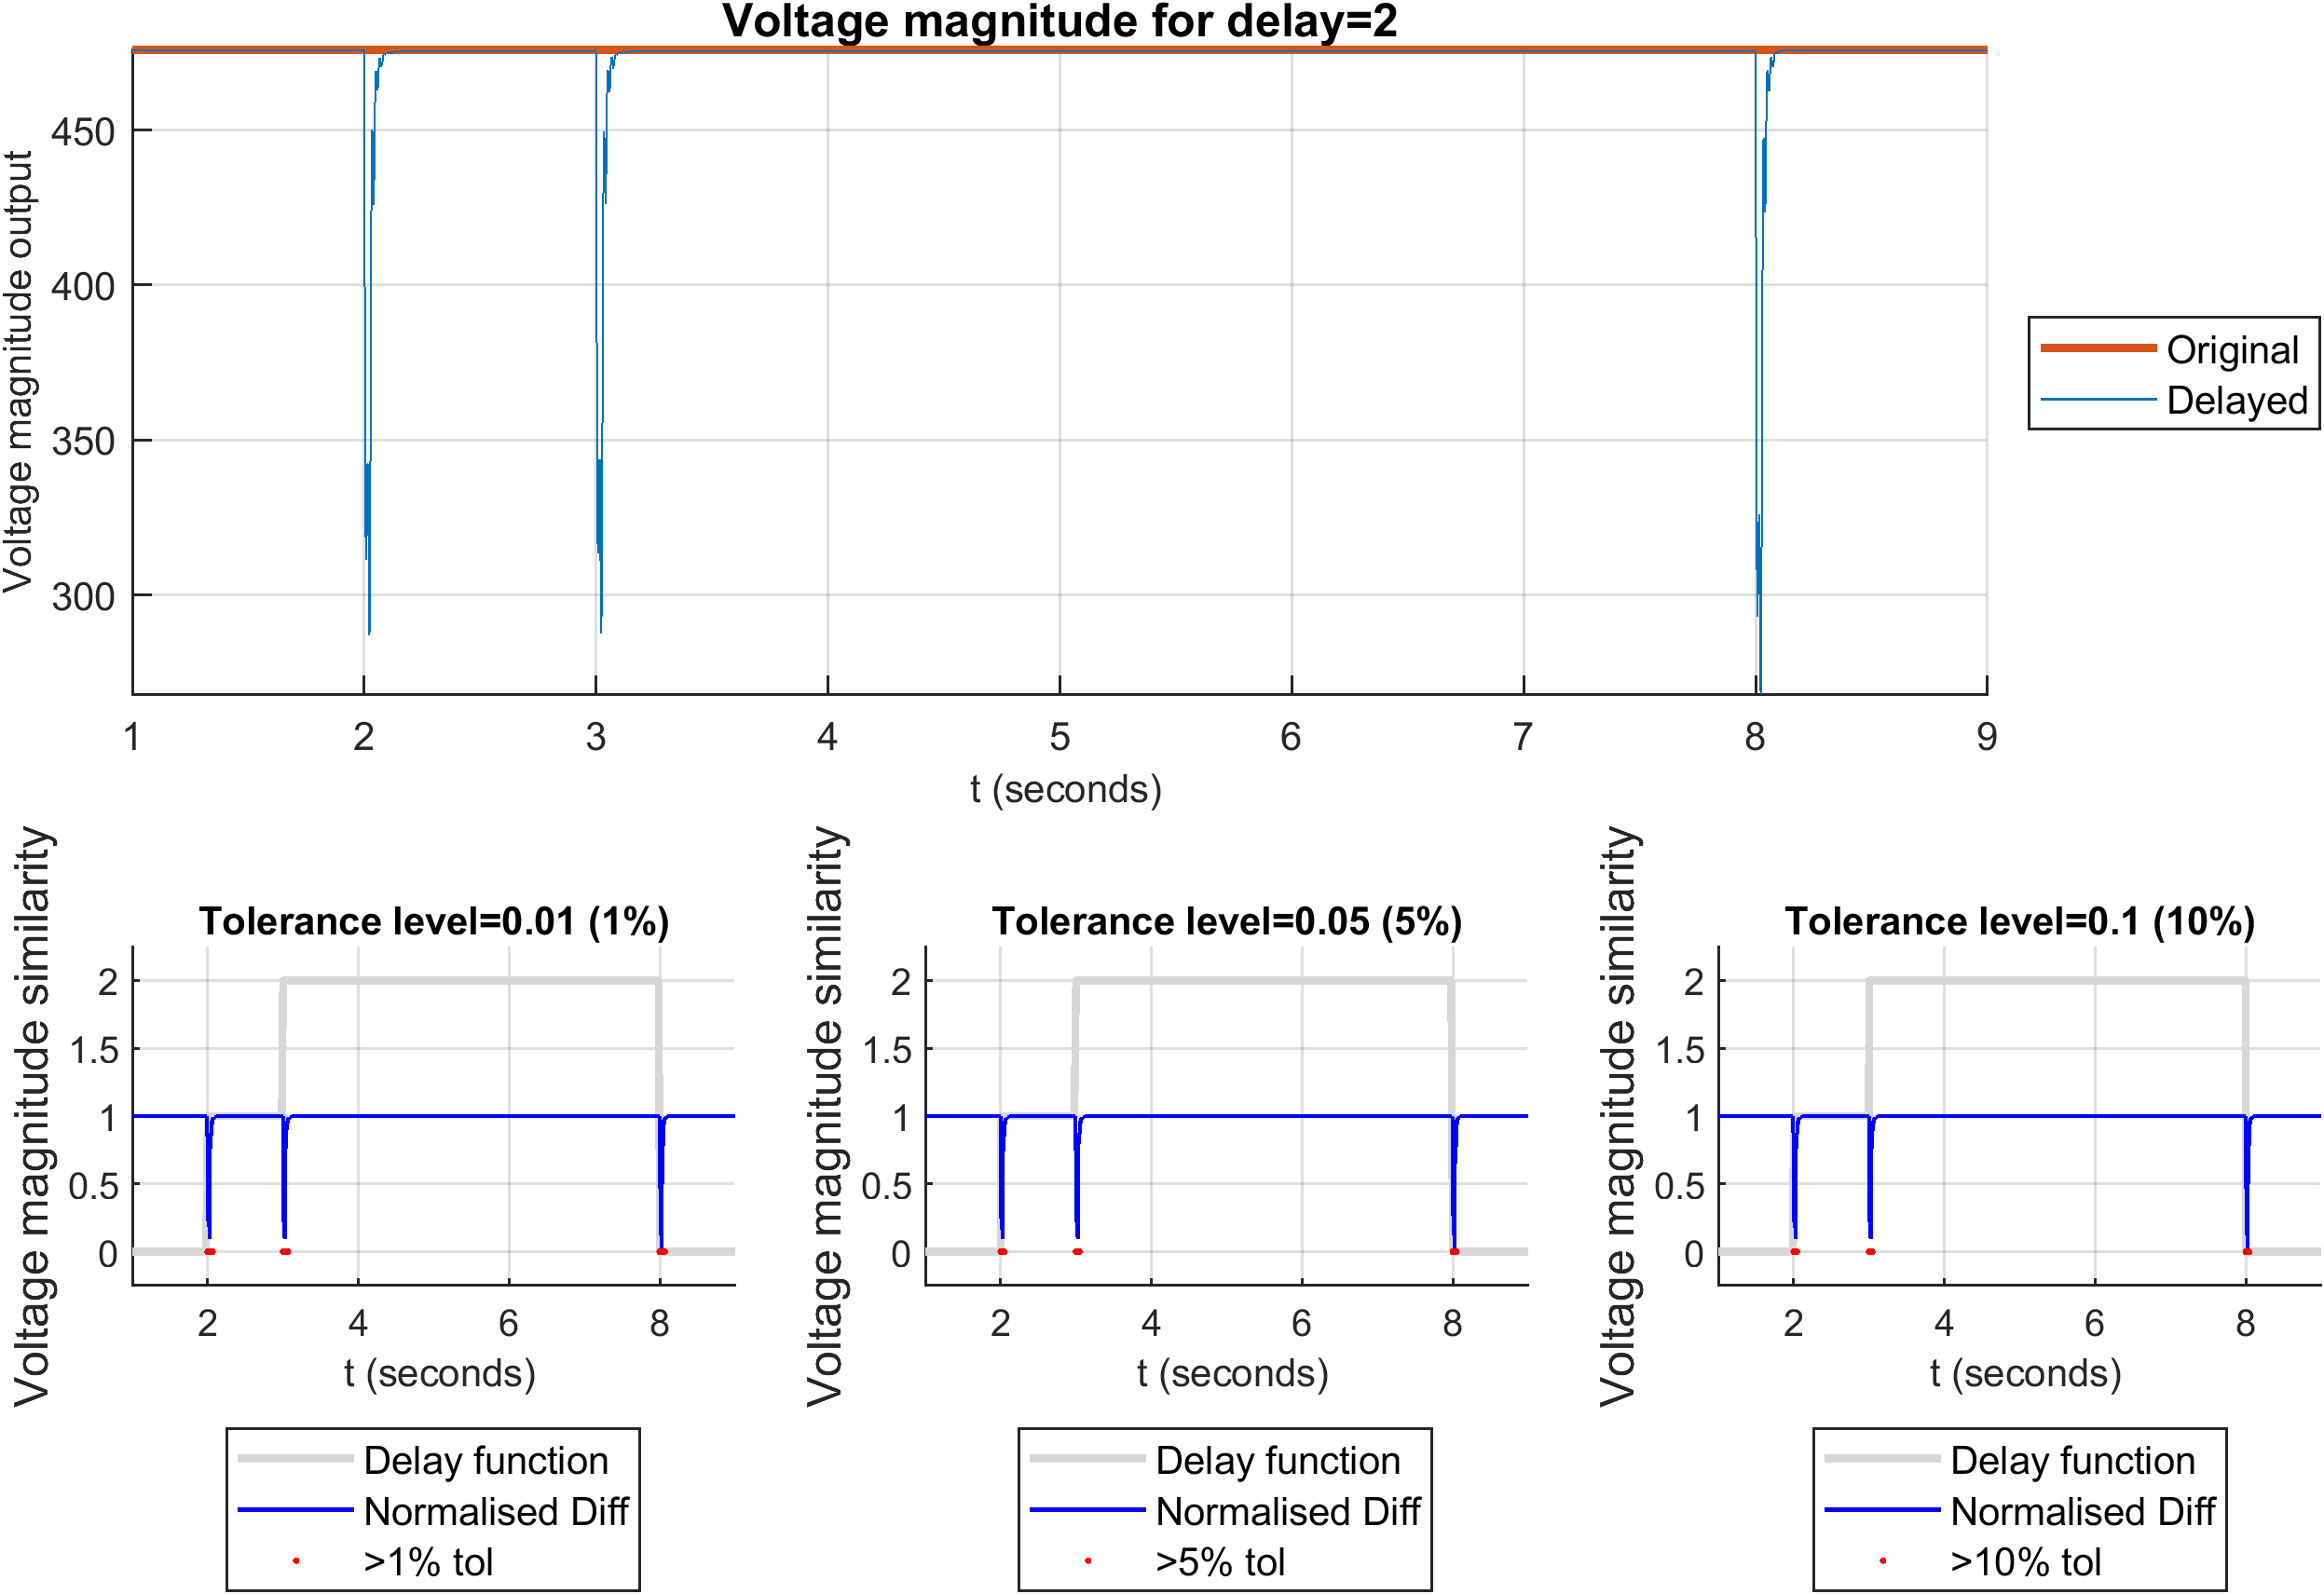
\includegraphics[width=0.95\textwidth]{PMUsim-figures/DelayOf_2/Step_vMagnitude.png}}\\
    \\ 
    
   \fbox{  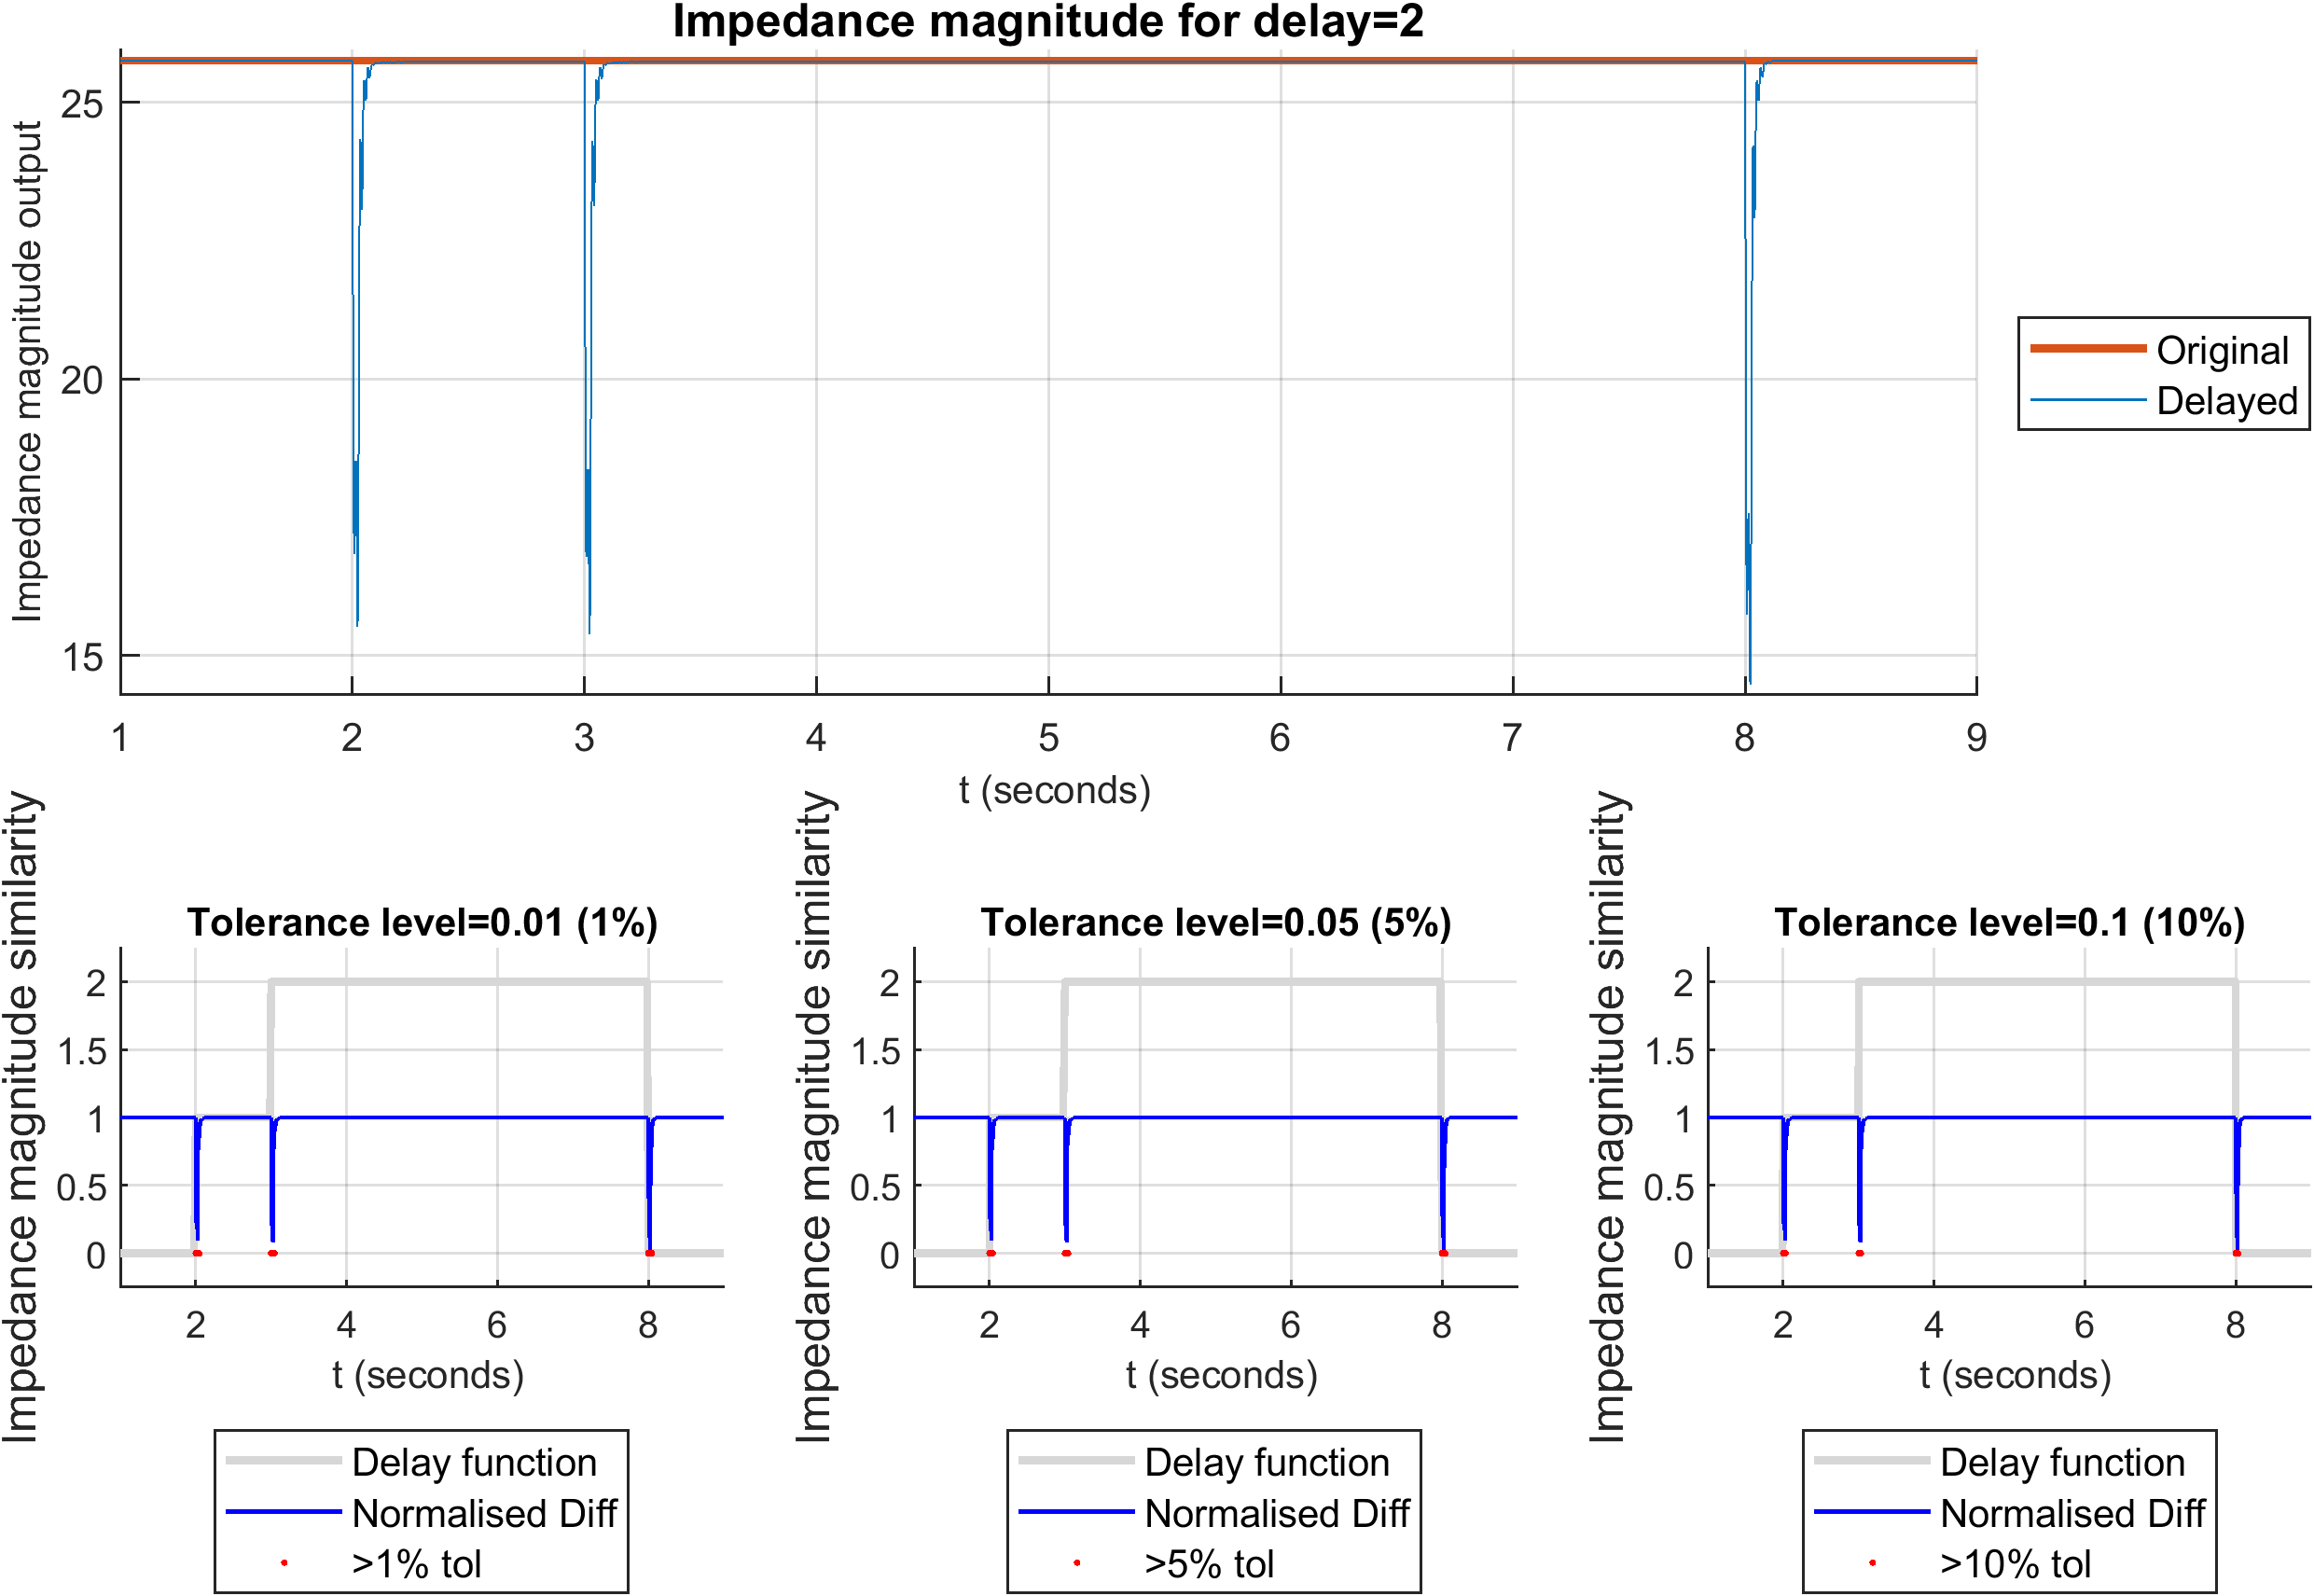
\includegraphics[width=0.95\textwidth]{PMUsim-figures/DelayOf_2/Step_iMagnitude.png}}\\
 \label{fig:PMUsimStep_Two_Mag}
 %\caption{Step-Wise Delay Magnitude Output for the Delay Level of Two}
  \end{tabular}
\caption[Step-Wise delay of 2: Magnitude Output]{Results for Magnitude Output for Step-Wise Delay equal to Two}
 \end{figure}
 
\newpage
\begin{figure}[H]
\begin{tabular}{c}
   \fbox{    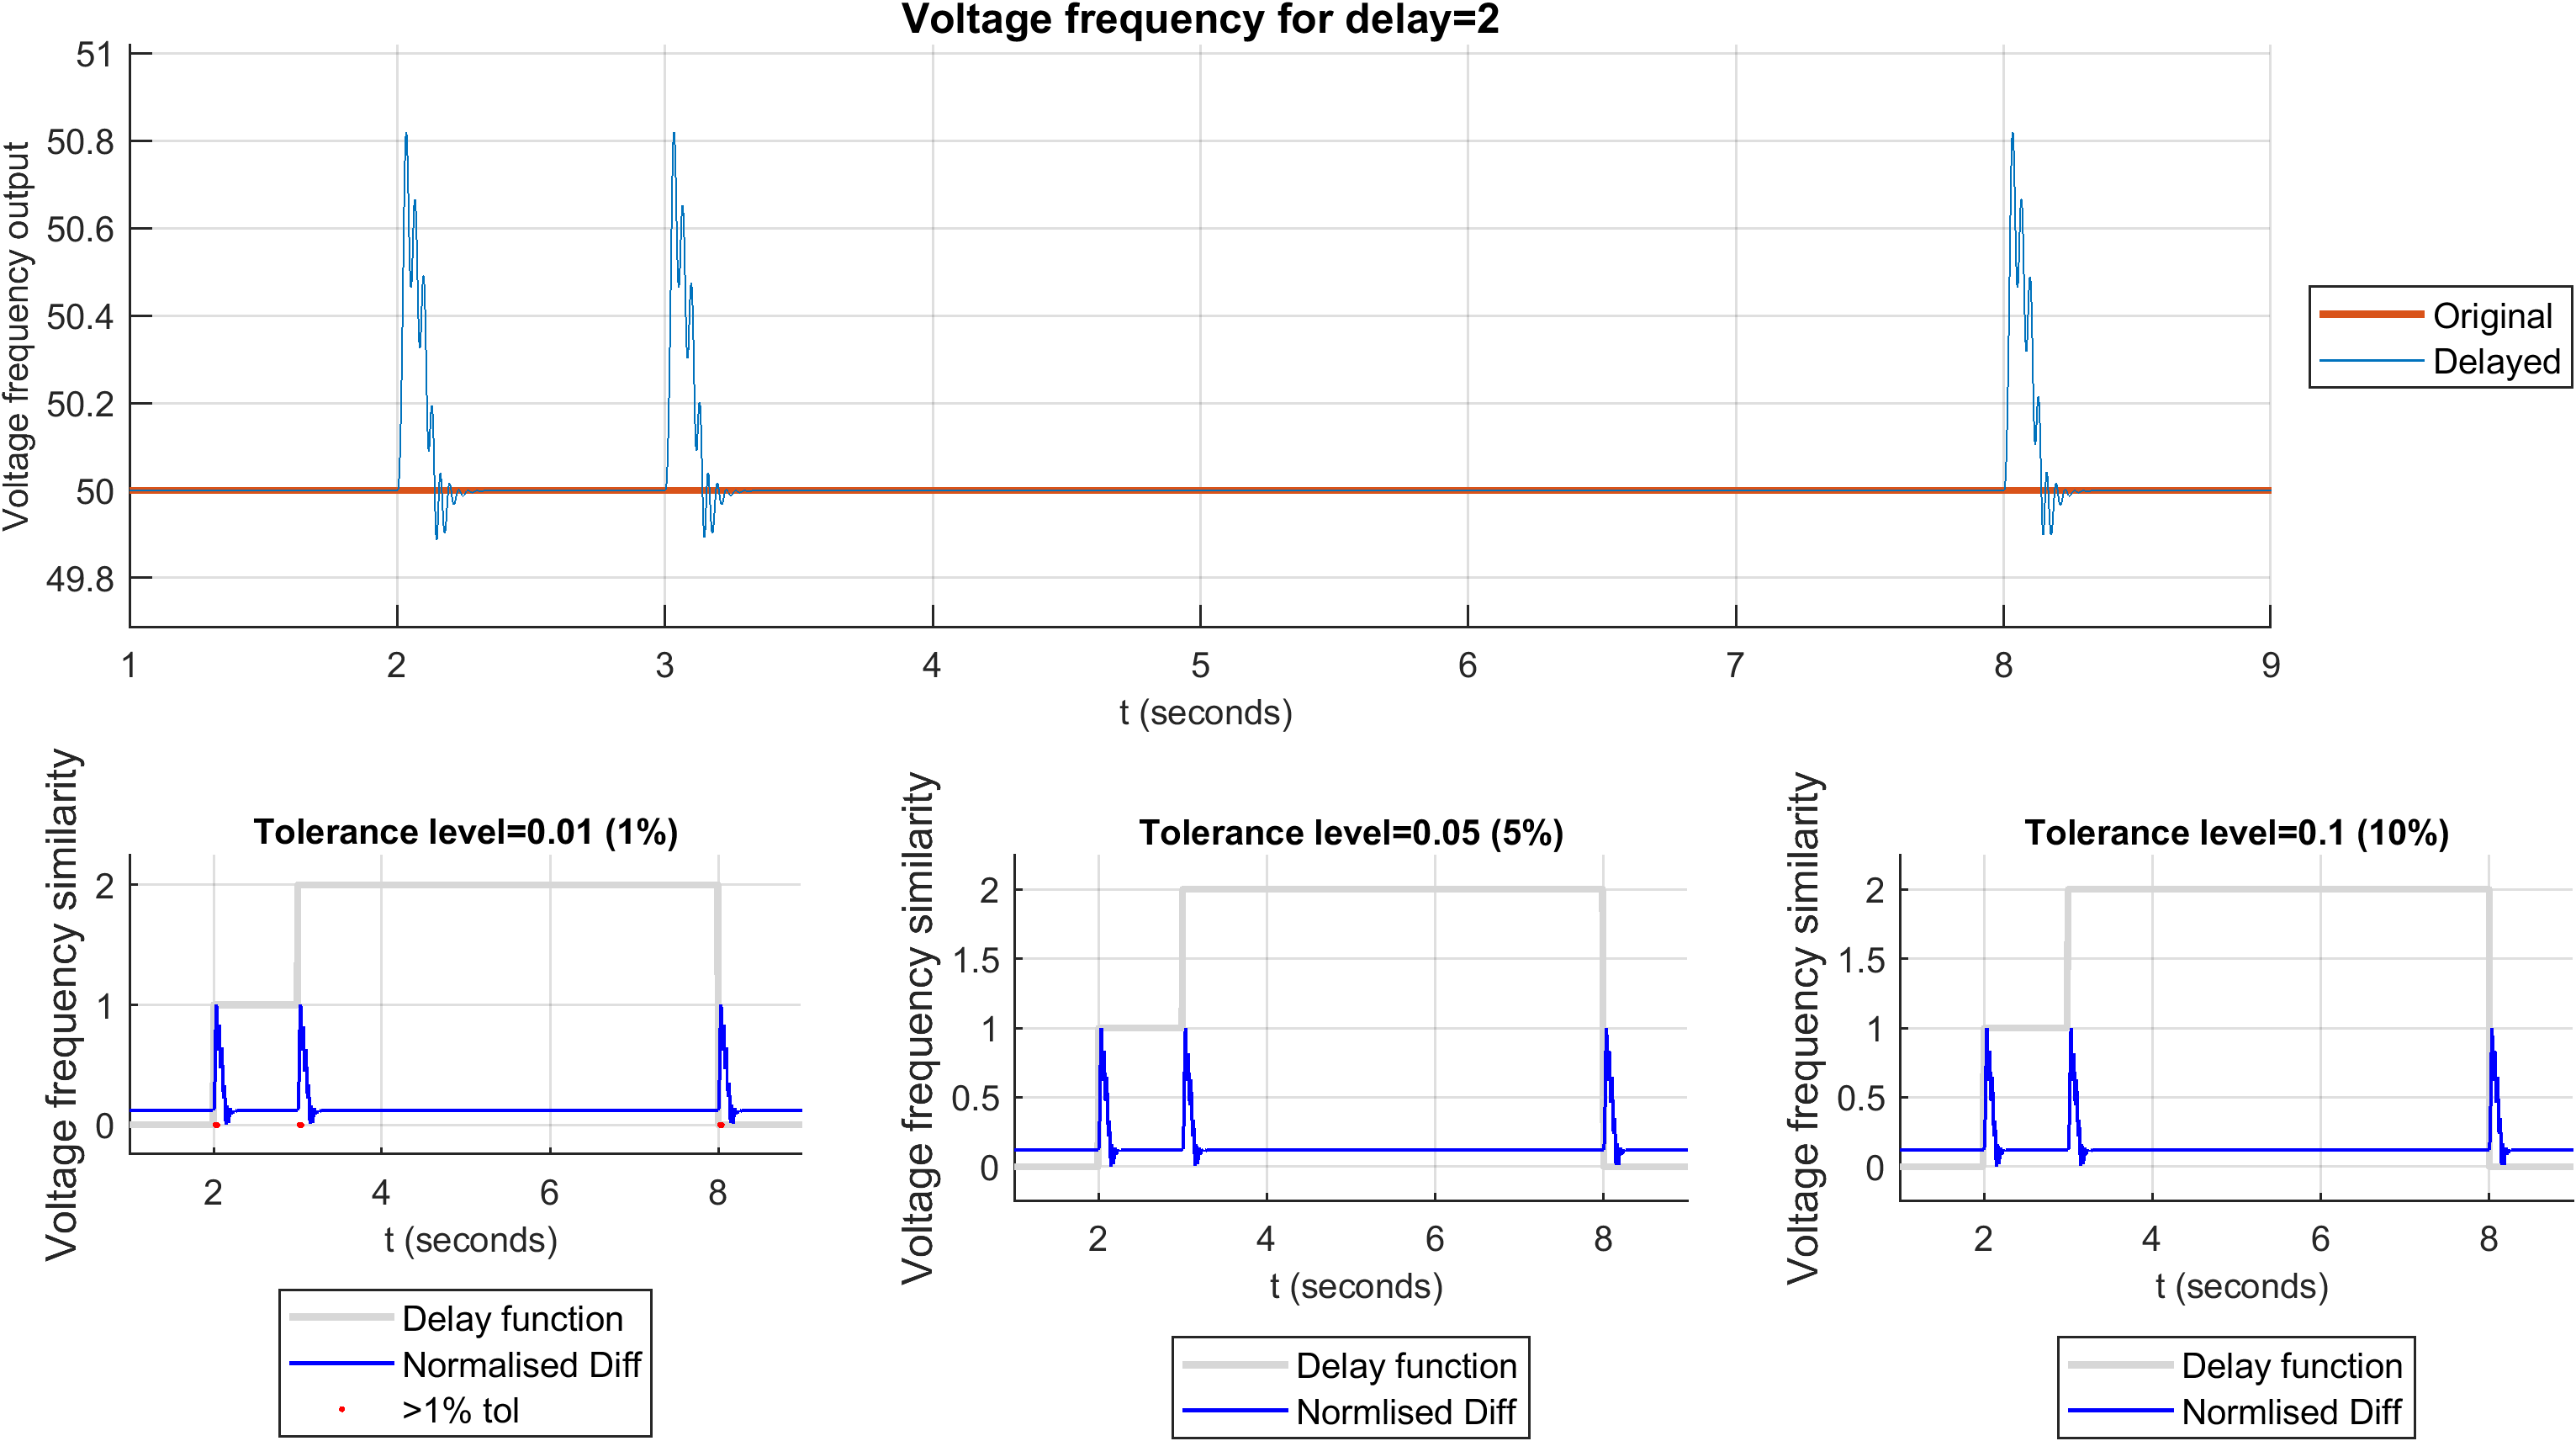
\includegraphics[width=0.95\textwidth]{PMUsim-figures/DelayOf_2/Step_vFrequency.png}}\\
    \\ 
    
   \fbox{  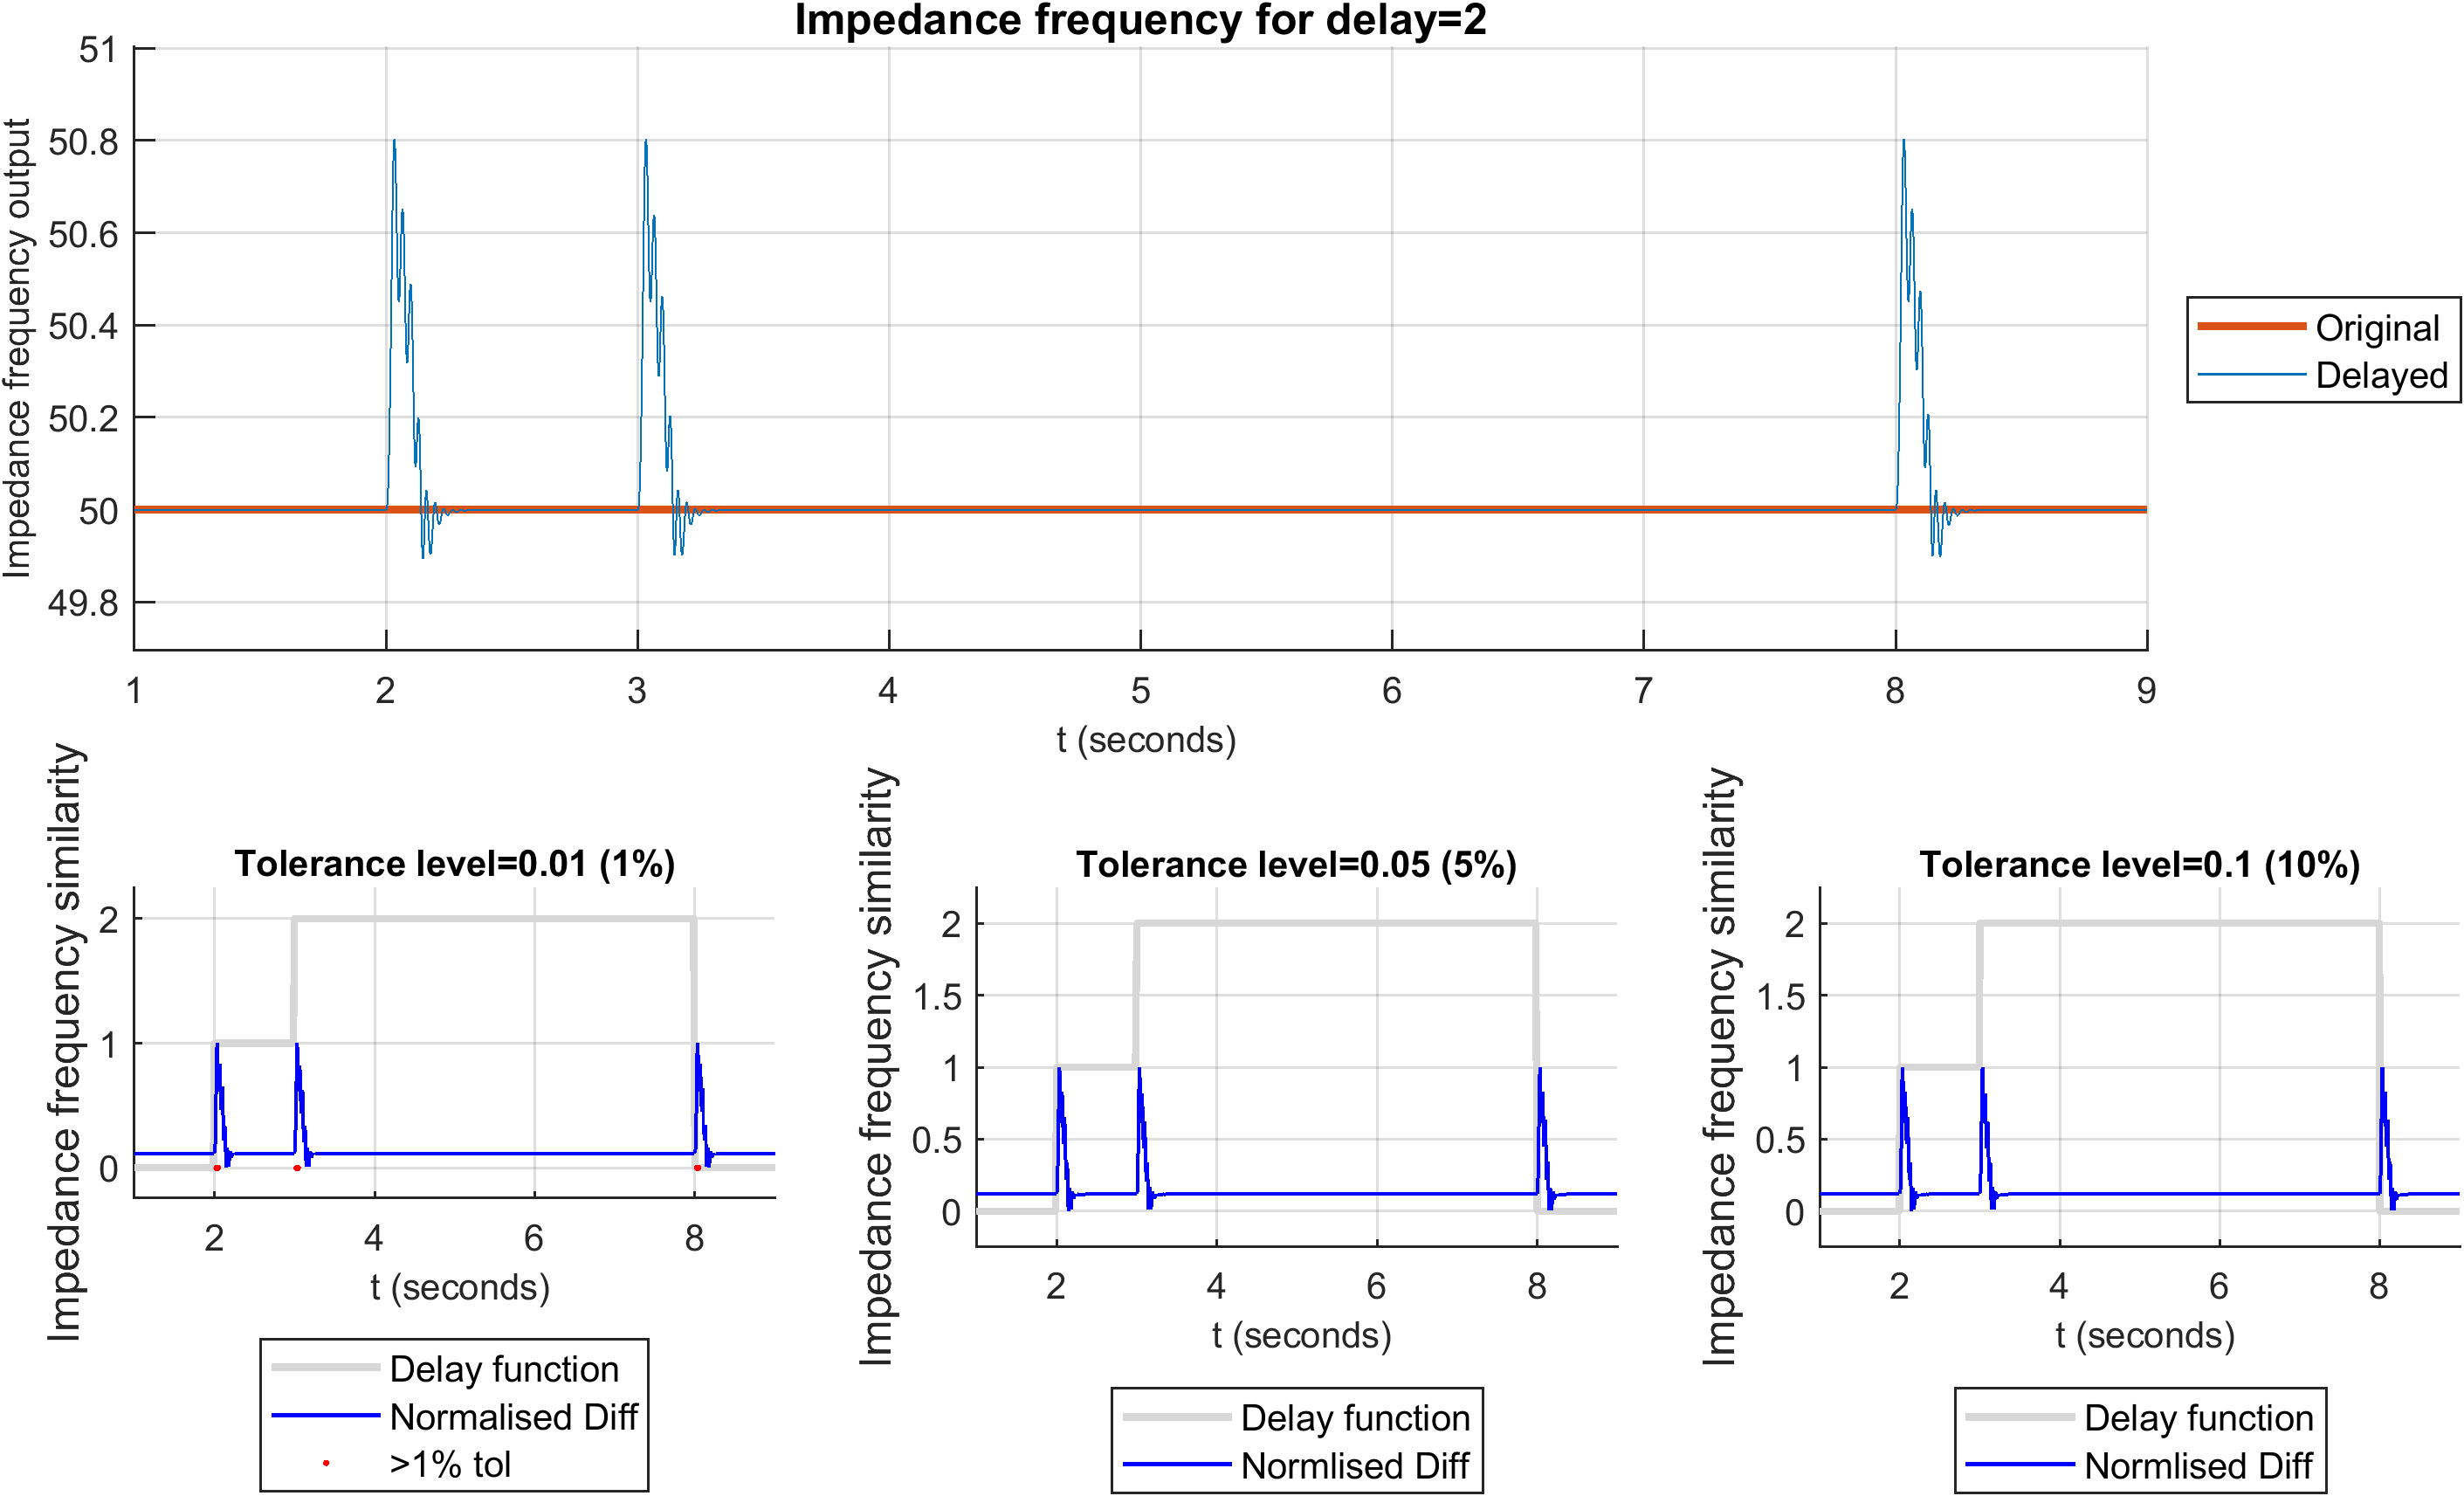
\includegraphics[width=0.95\textwidth]{PMUsim-figures/DelayOf_2/Step_iFrequency.png}}\\
 \label{fig:PMUsimStep_Two_Freq}
 %\caption{Step-Wise Delay Frequency Output for the Delay Level of Two}
  \end{tabular}
\caption[Step-Wise delay of 2: Frequency Output]{Results for Frequency Output for Step-Wise Delay equal to Two}
 \end{figure}
 


\newpage
\begin{figure}[H]
\begin{tabular}{c}
   \fbox{     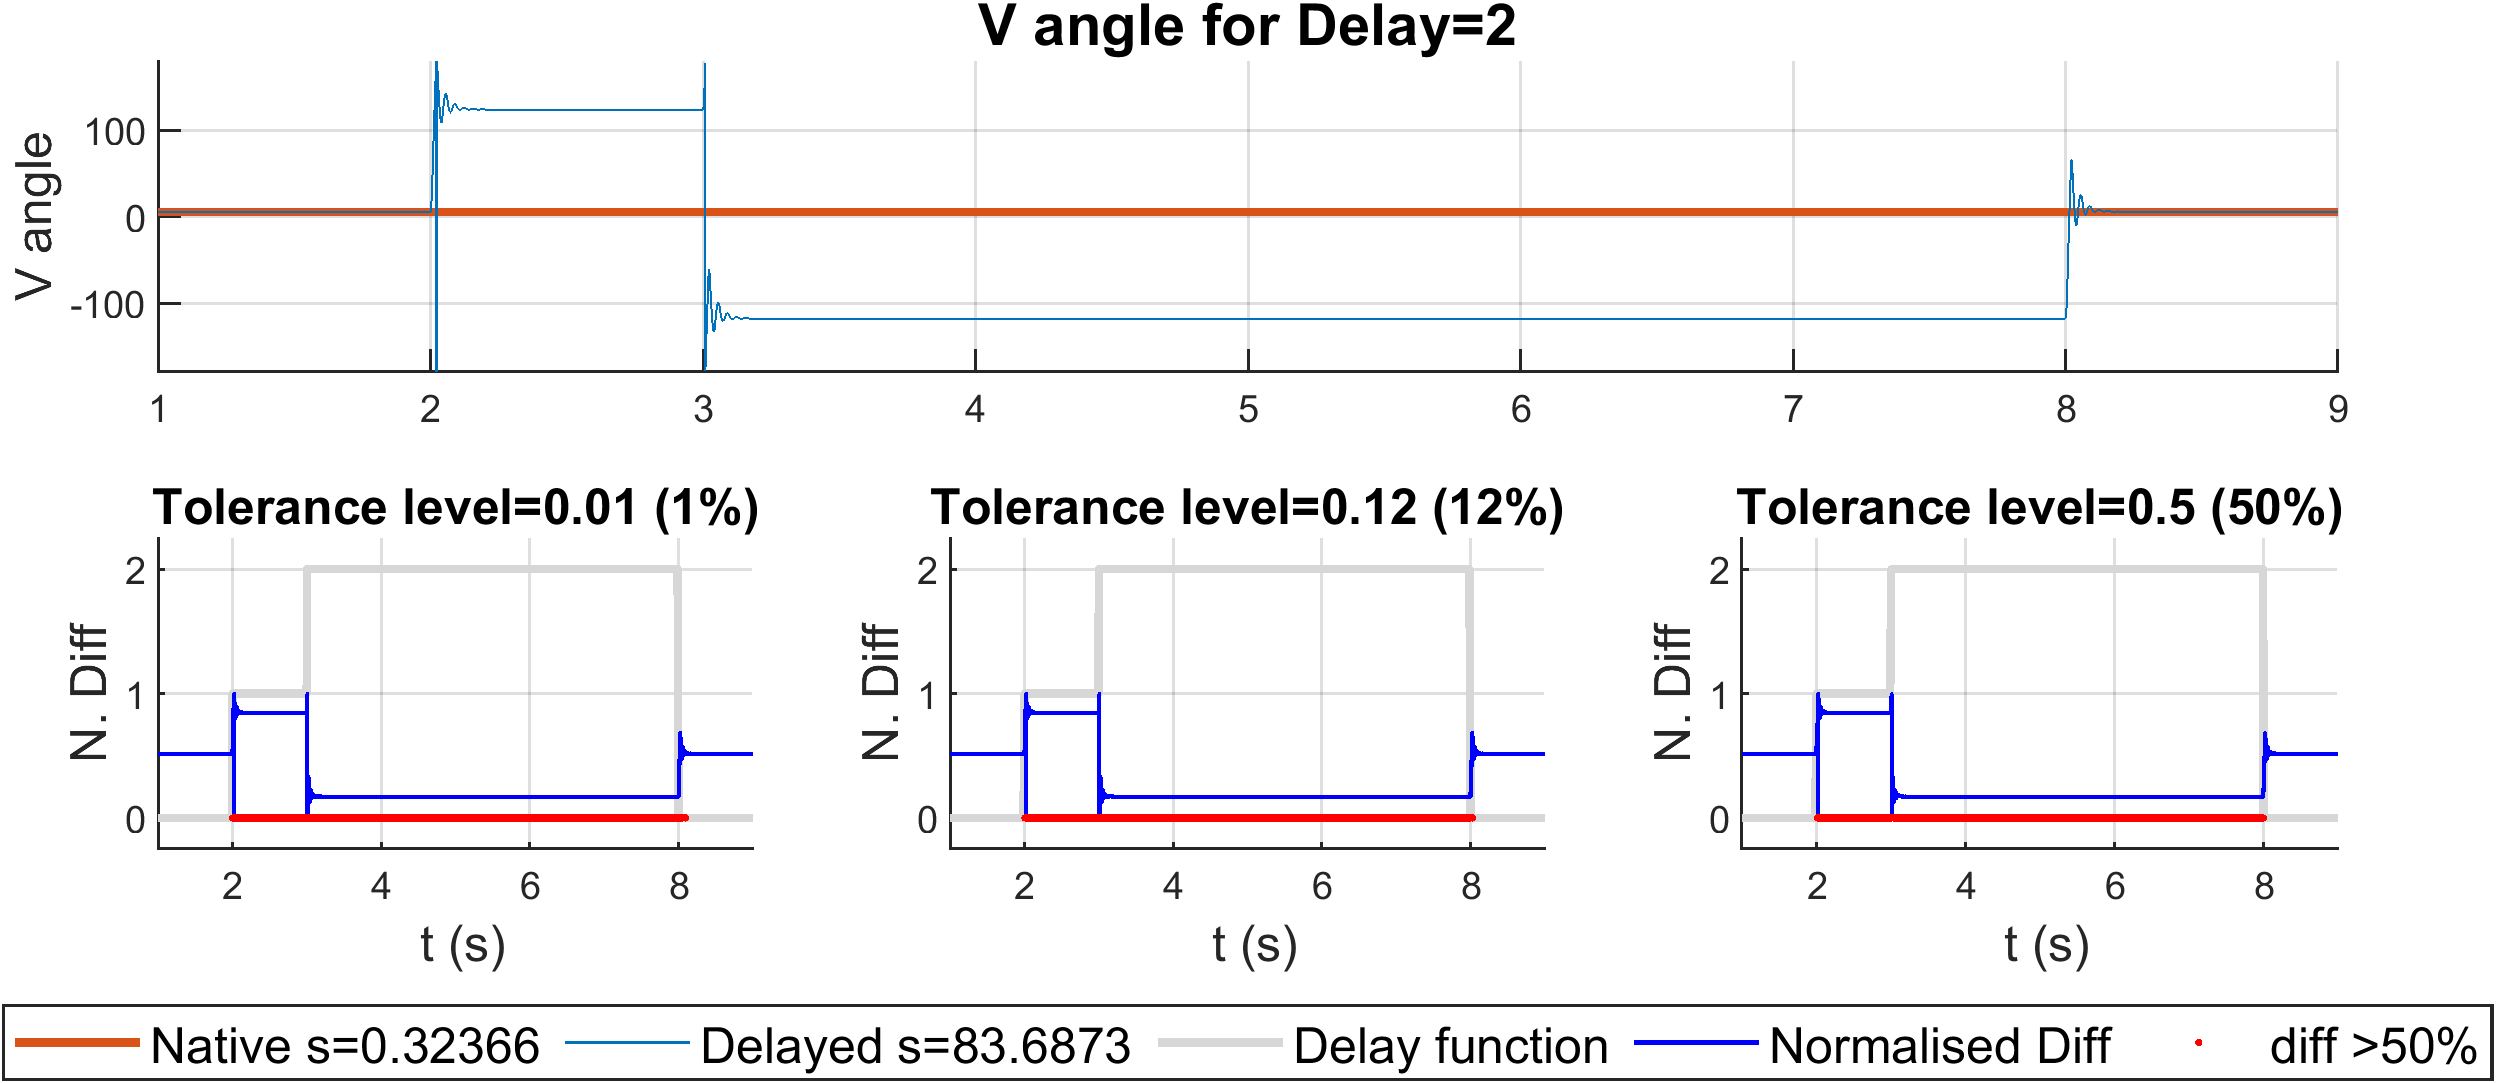
\includegraphics[width=0.95\textwidth]{PMUsim-figures/DelayOf_2/Step_vAngle.png}}\\
    \\ 
    
   \fbox{ 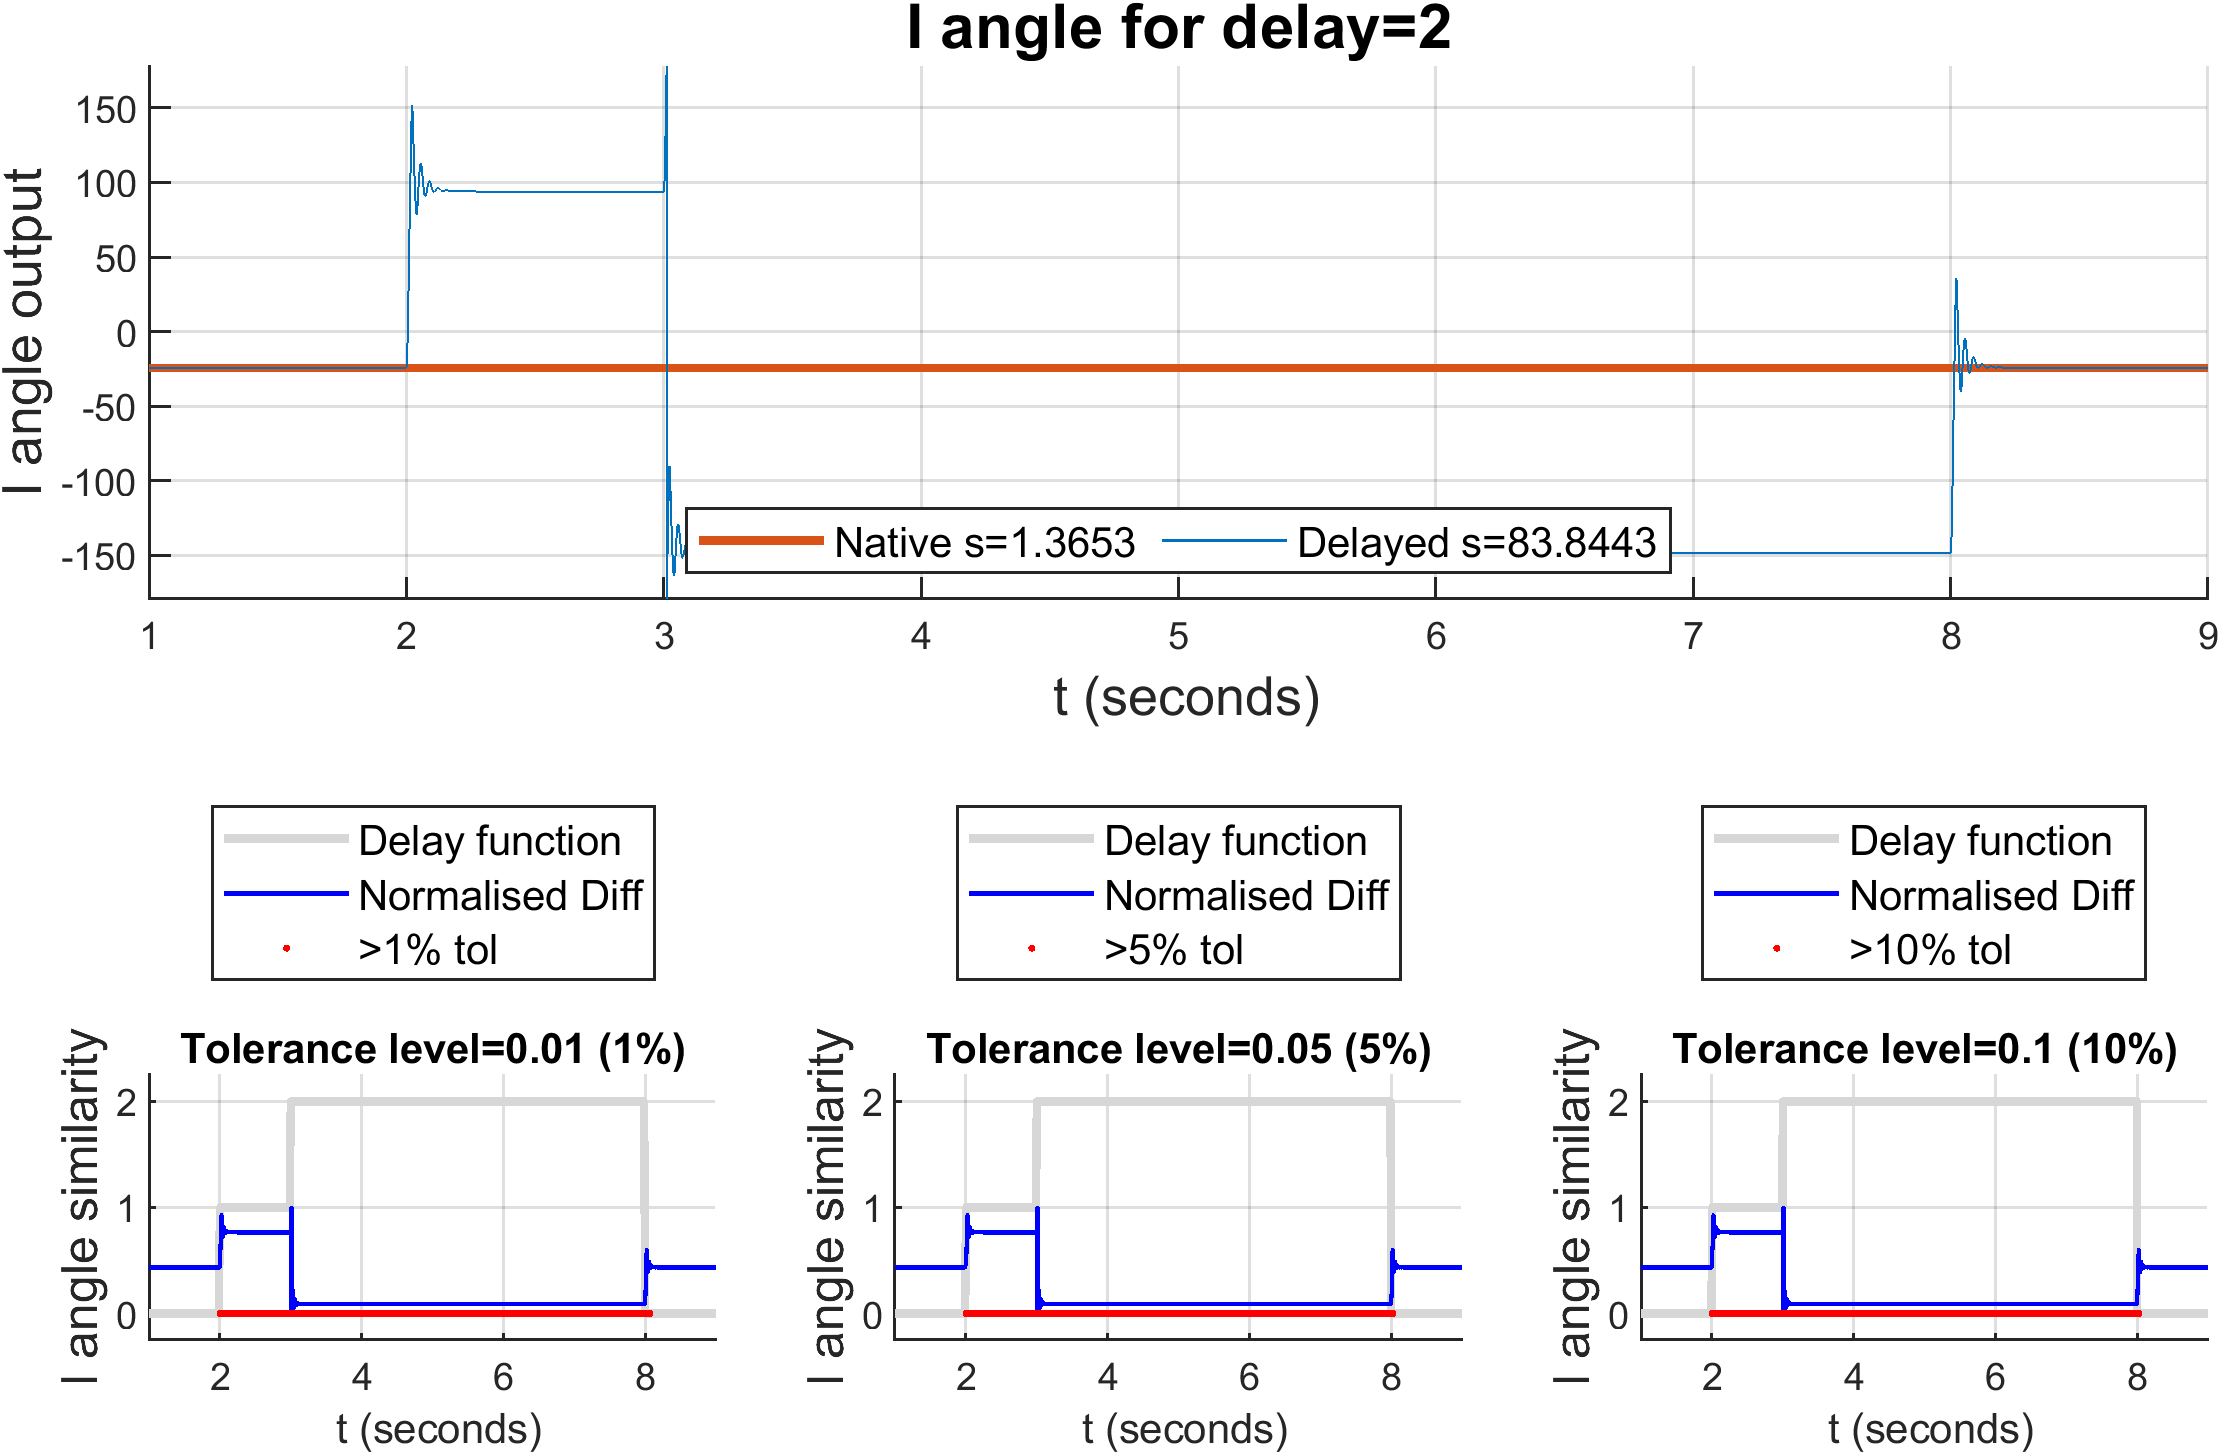
\includegraphics[width=0.95\textwidth]{PMUsim-figures/DelayOf_2/Step_iAngle.png}}\\
 \label{fig:PMUsimStep_Two_Angle}
 %\caption{Step-Wise Delay Angle Output for the Delay Level of Two}
  \end{tabular}
\caption[Step-Wise delay of 2: Angle Output]{Results for Angle Output for Step-Wise Delay equal to Two}
 \end{figure}


\newpage \subsection{Step-Wise Delay Level of Three}

 \begin{small}
    \tcbox[size=normal, standard jigsaw, opacityback=0, boxrule=0pt,halign=justify]{
     Step-Wise Delay Level of Three}{
          \begin{itemize}
         \item      The delayed signal (blue) overlaps the original signal (red), producing a straight line, colored neither red nor blue.
         \item  The blue Normalised diff signal also overlaps the grey delay function.
          \end{itemize} }
\end{small}

\begin{figure}[H]
\begin{tabular}{c}
   \fbox{    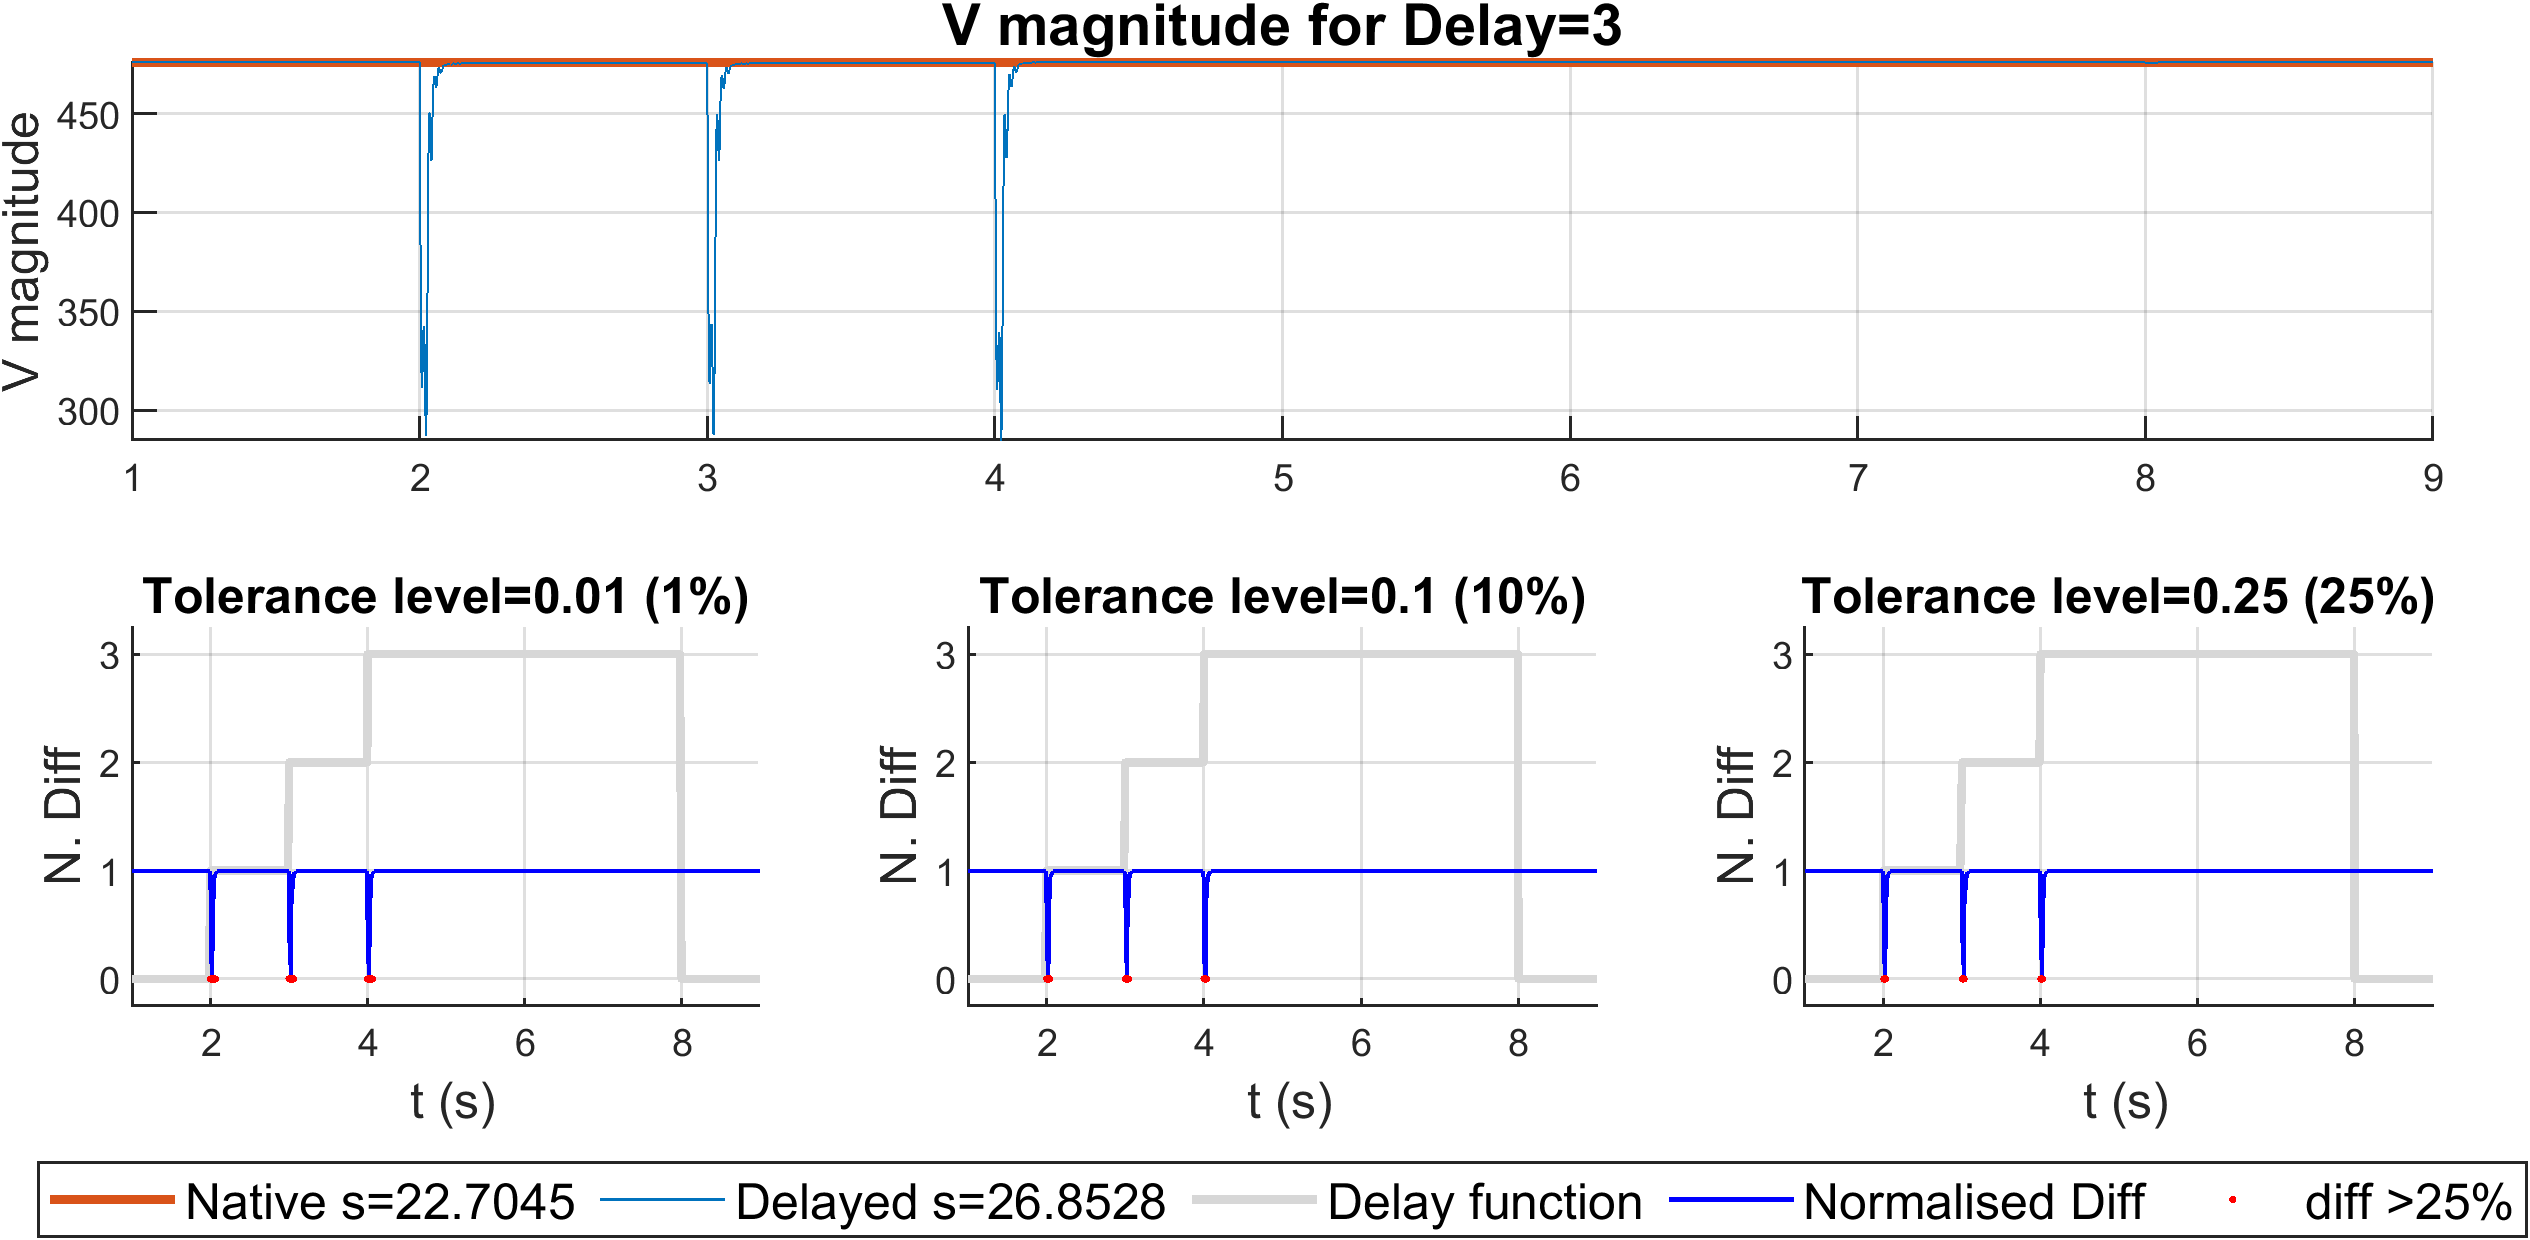
\includegraphics[width=0.95\textwidth]{PMUsim-figures/DelayOf_3/Step_vMagnitude.png}}\\
  
     \\  
   \fbox{  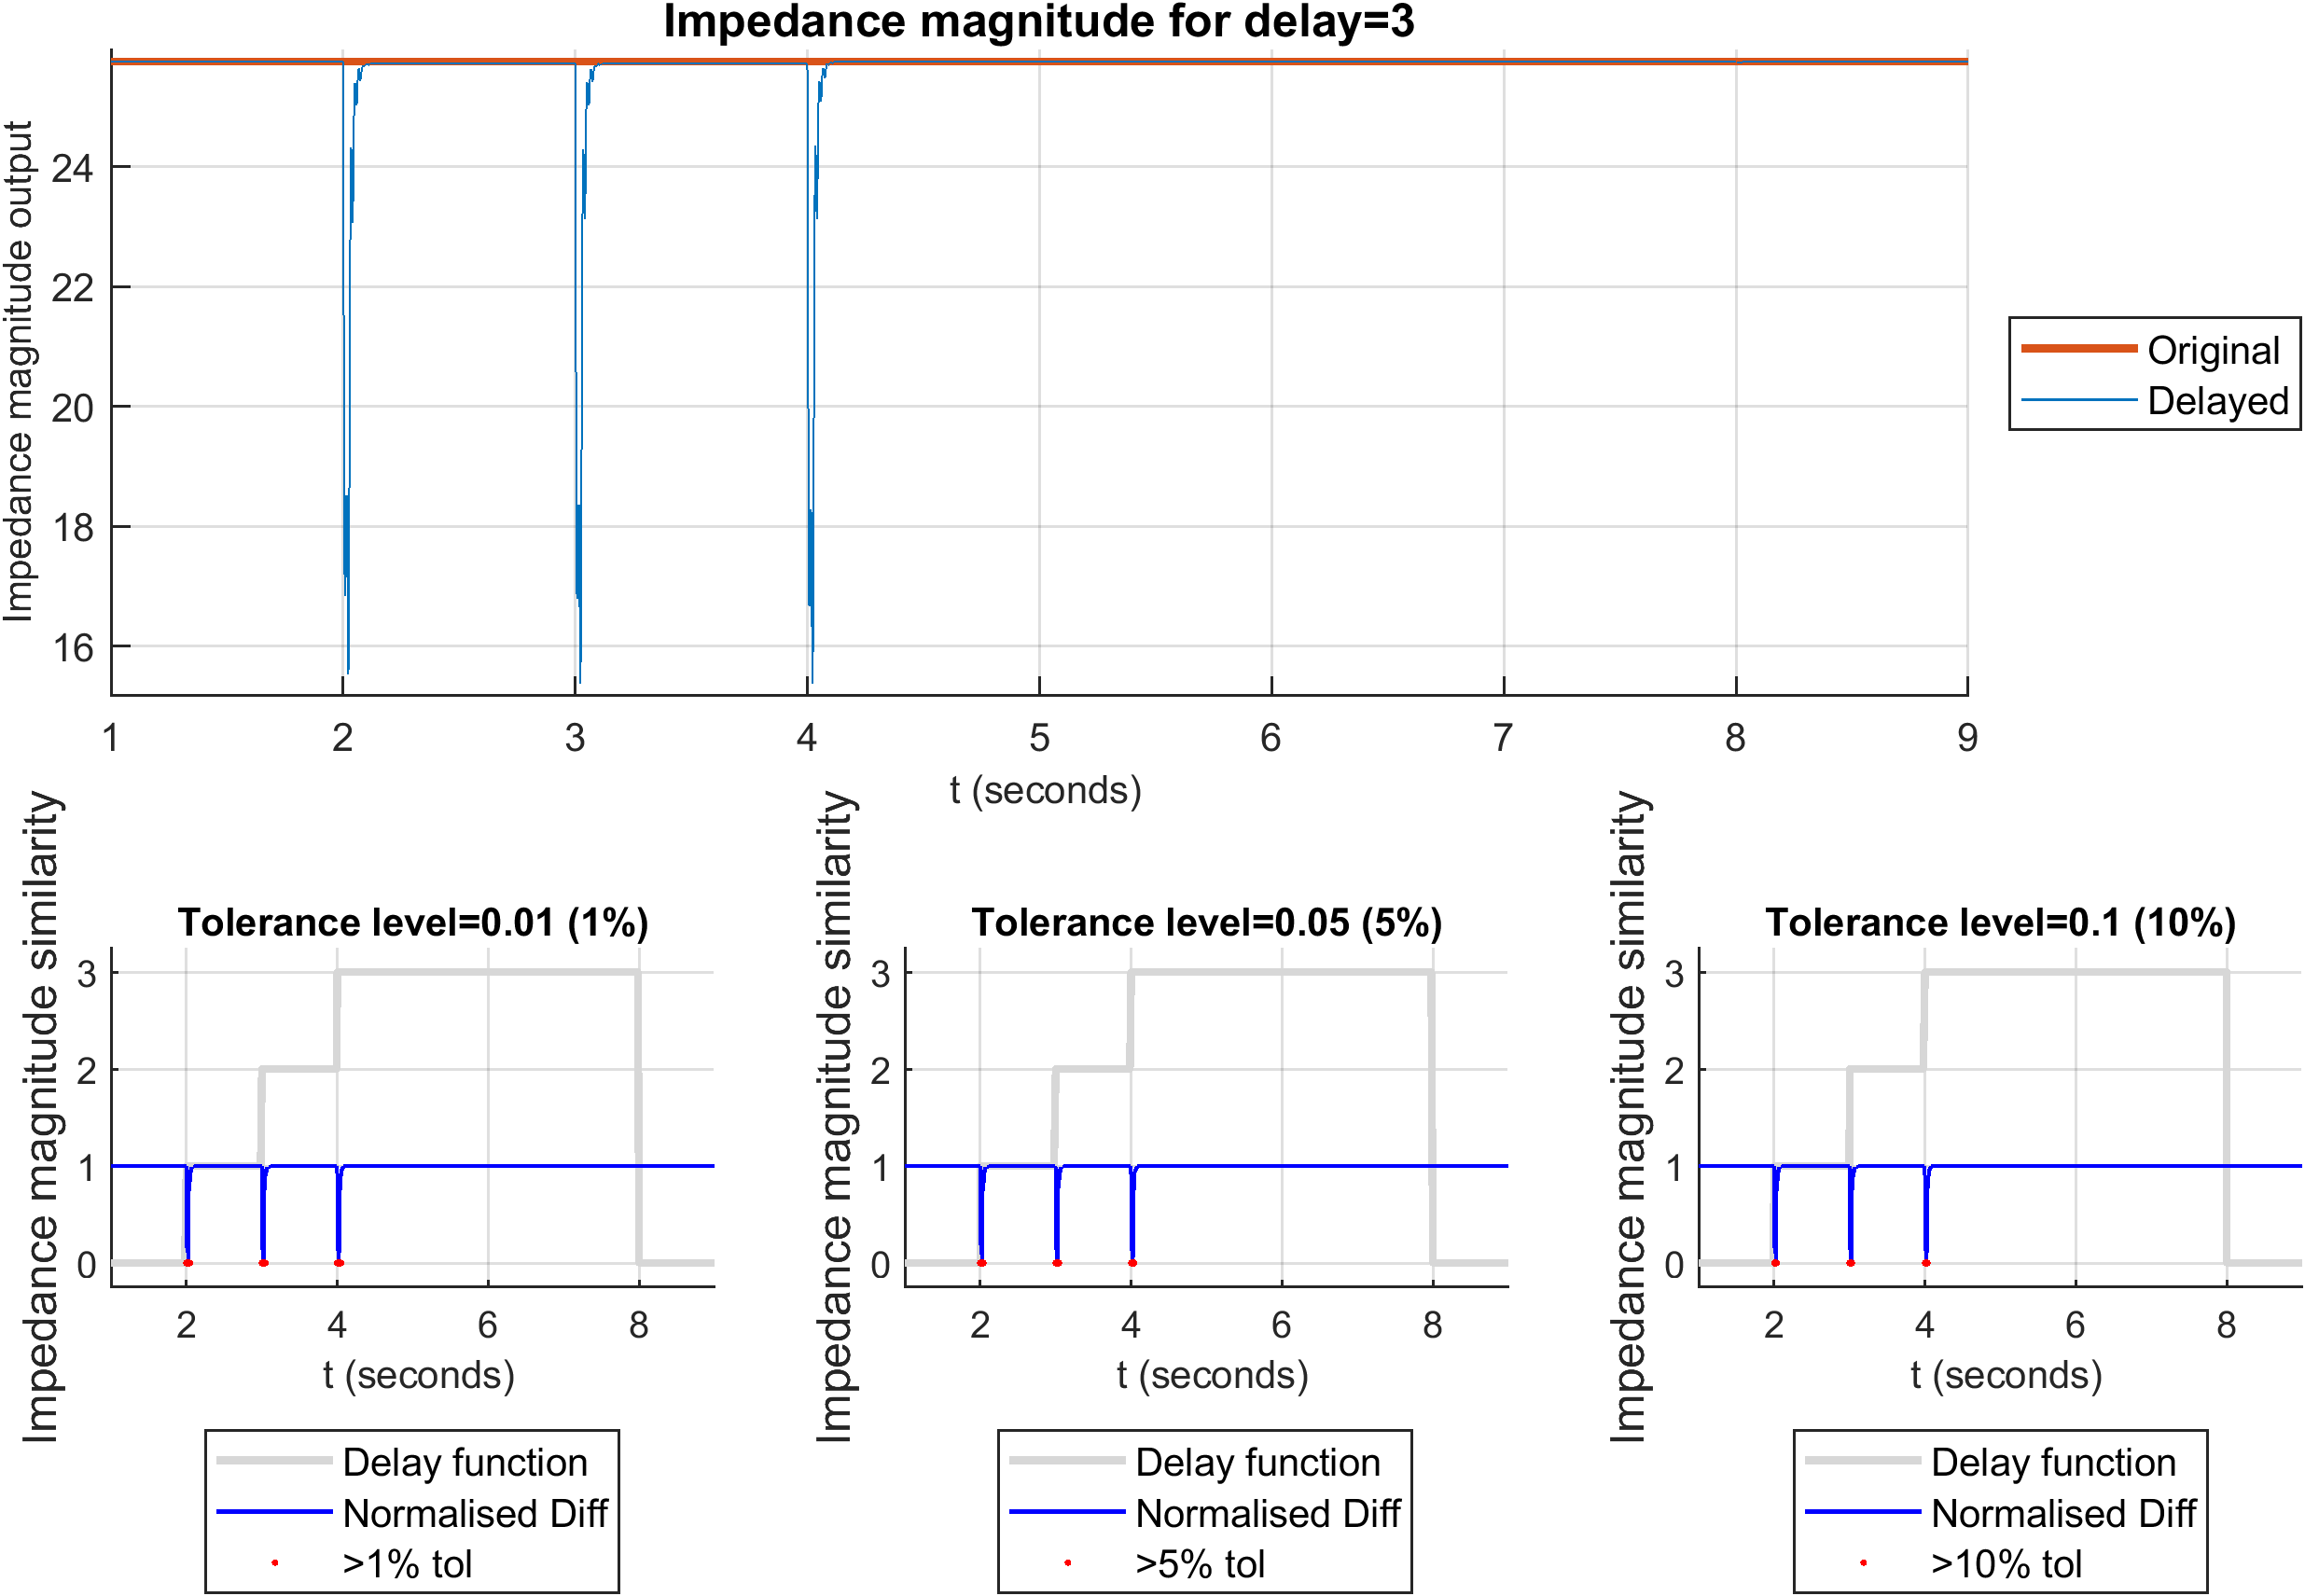
\includegraphics[width=0.95\textwidth]{PMUsim-figures/DelayOf_3/Step_iMagnitude.png}}\\
 \label{fig:PMUsimStep_Three_Mag}
 %\caption{Step-Wise Delay Magnitude Output for the Delay Level of Three}
  \end{tabular}
\caption[Step-Wise delay of 3: Magnitude Output]{Results for Magnitude Output for Step-Wise Delay equal to Three}
 \end{figure}



\newpage 

\begin{figure}[H]
\begin{tabular}{c}
   \fbox{     \includegraphics[width=0.95\textwidth]{PMUsim-figures/DelayOf_3/Step_vFrequency.png}}\\
   \\  
    
   \fbox{  \includegraphics[width=0.95\textwidth]{PMUsim-figures/DelayOf_3/Step_iFrequency.png}}\\
 \label{fig:PMUsimStep_Three_Freq}
 %\caption{Step-Wise Delay Frequency Output for the Delay Level of Three}
  \end{tabular}
\caption[Step-Wise delay of 3: Frequency Output]{Results for Frequency Output for Step-Wise Delay equal to Three}
 \end{figure}




\newpage 

\begin{figure}[H]
\begin{tabular}{c}
   \fbox{      \includegraphics[width=0.95\textwidth]{PMUsim-figures/DelayOf_3/Step_vAngle.png}}\\
    \\ 
    
   \fbox{  \includegraphics[width=0.95\textwidth]{PMUsim-figures/DelayOf_3/Step_iAngle.png}}\\
 \label{fig:PMUsimStep_Three_Angle}
 %\caption{Step-Wise Delay Angle Output for the Delay Level of Three}
  \end{tabular}
\caption[Step-Wise delay of 3: Angle Output]{Results for Angle Output for Step-Wise Delay equal to Three}
 \end{figure}


\newpage\subsection{Step-Wise Delay Level of Four}

 \begin{small}
    \tcbox[size=normal, standard jigsaw, opacityback=0, boxrule=0pt,halign=justify]{
     Step-Wise Delay Level of Four}{
          \begin{itemize}
         \item      The delayed signal (blue) overlaps the original signal (red), producing a straight line, colored neither red nor blue.
         \item  The blue Normalised diff signal also overlaps the grey delay function.
          \end{itemize} }
\end{small}

\begin{figure}[H]
\begin{tabular}{c}

   \fbox{    \includegraphics[width=0.95\textwidth]{PMUsim-figures/DelayOf_4/Step_vMagnitude.png}}\\
   \\
    
   \fbox{   \includegraphics[width=0.95\textwidth]{PMUsim-figures/DelayOf_4/Step_iMagnitude.png}}\\
 \label{fig:PMUsimStep_Four_Mag}
 %\caption{Step-Wise Delay Magnitude Output for the Delay Level of Four}
  \end{tabular}
\caption[Step-Wise delay of 4: Magnitude Output]{Results for Magnitude Output for Step-Wise Delay equal to Four}
 \end{figure}



\newpage 

\begin{figure}[H]
\begin{tabular}{c}
   \fbox{    \includegraphics[width=0.95\textwidth]{PMUsim-figures/DelayOf_4/Step_vFrequency.png}}\\
   \\ 
    
   \fbox{  \includegraphics[width=0.95\textwidth]{PMUsim-figures/DelayOf_4/Step_iFrequency.png}}\\
 \label{fig:PMUsimStep_Four_Freq}
 %\caption{Step-Wise Delay Frequency Output for the Delay Level of Four}
  \end{tabular}
\caption[Step-Wise delay of 4: Frequency Output]{Results for Frequency Output for Step-Wise Delay equal to Four}
 \end{figure}




\newpage 

\begin{figure}[H]
\begin{tabular}{c}
   \fbox{     \includegraphics[width=0.95\textwidth]{PMUsim-figures/DelayOf_4/Step_vAngle.png}}\\
    \\ 
    
   \fbox{   \includegraphics[width=0.95\textwidth]{PMUsim-figures/DelayOf_4/Step_iAngle.png}}\\
 \label{fig:PMUsimStep_Four_Angle}
 %\caption{Step-Wise Delay Angle Output for the Delay Level of Four}
  \end{tabular}
\caption[Step-Wise delay of 4: Angle Output]{Results for Angle Output for Step-Wise Delay equal to Four}
 \end{figure}


\newpage \subsection{Step-Wise Delay Level of Five}

 \begin{small}
    \tcbox[size=normal, standard jigsaw, opacityback=0, boxrule=0pt,halign=justify]{
     Step-Wise Delay Level of Five}{
          \begin{itemize}
         \item      The delayed signal (blue) overlaps the original signal (red), producing a straight line, colored neither red nor blue.
         \item  The blue Normalised diff signal also overlaps the grey delay function.
          \end{itemize} }
\end{small}

\begin{figure}[H]
\begin{tabular}{c}
   \fbox{     \includegraphics[width=0.95\textwidth]{PMUsim-figures/DelayOf_5/Step_vMagnitude.png}}\\
    \\ 
    
   \fbox{   \includegraphics[width=0.95\textwidth]{PMUsim-figures/DelayOf_5/Step_iMagnitude.png}}\\
 \label{fig:PMUsimStep_Five_Mag}
 %\caption{Step-Wise Delay Magnitude Output for the Delay Level of Five}
  \end{tabular}
\caption[Step-Wise delay of 5: Magnitude Output]{Results for Magnitude Output for Step-Wise Delay equal to Five}
 \end{figure}


\newpage 

\begin{figure}[H]
\begin{tabular}{c}
   \fbox{     \includegraphics[width=0.95\textwidth]{PMUsim-figures/DelayOf_5/Step_vFrequency.png}}\\
    \\ 
    
   \fbox{  \includegraphics[width=0.95\textwidth]{PMUsim-figures/DelayOf_5/Step_iFrequency.png}}\\
 \label{fig:PMUsimStep_Five_Freq}
 %\caption{Step-Wise Delay Frequency Output for the Delay Level of Five}
  \end{tabular}
\caption[Step-Wise delay of 5: Frequency Output]{Results for Frequency Output for Step-Wise Delay equal to Five}
 \end{figure}


\newpage 

\begin{figure}[H]
\begin{tabular}{c} 
   \fbox{    \includegraphics[width=0.95\textwidth]{PMUsim-figures/DelayOf_5/Step_vAngle.png}}\\
    \\ 
    
   \fbox{   \includegraphics[width=0.95\textwidth]{PMUsim-figures/DelayOf_5/Step_iAngle.png}}\\  
 \label{fig:PMUsimStep_Five_Angle}
 %\caption{Step-Wise Delay Angle Output for the Delay Level of Five}
  \end{tabular}
\caption[Step-Wise delay of 5: Angle Output]{Results for Angle Output for Step-Wise Delay equal to Five}
 \end{figure}



\newpage 
\subsection{Step-Wise Delay Level of Six} 


 \begin{small}
    \tcbox[size=normal, standard jigsaw, opacityback=0, boxrule=0pt,halign=justify]{
     Step-Wise Delay Level of Six}{
          \begin{itemize}
         \item      The delayed signal (blue) overlaps the original signal (red), producing a straight line, colored neither red nor blue.
         \item  The blue Normalised diff signal also overlaps the grey delay function.
          \end{itemize} }
\end{small}


\newpage 
\begin{figure}[H]
\begin{tabular}{c} 
   \fbox{     \includegraphics[width=0.95\textwidth]{PMUsim-figures/DelayOf_6/Step_vMagnitude.png}}\\
    \\ 
    
   \fbox{   \includegraphics[width=0.95\textwidth]{PMUsim-figures/DelayOf_6/Step_iMagnitude.png}}\\
 \label{fig:PMUsimStep_Six_Mag}
 %\caption{Step-Wise Delay Magnitude Output for the Delay Level of Six}
  \end{tabular}
\caption[Step-Wise delay of 6: Magnitude Output]{Results for Magnitude Output for Step-Wise Delay equal to Six}
 \end{figure}



\newpage 
\begin{figure}[H]
\begin{tabular}{c} 
   \fbox{    \includegraphics[width=0.95\textwidth]{PMUsim-figures/DelayOf_6/Step_vFrequency.png}}\\
    \\ 
    
   \fbox{   \includegraphics[width=0.95\textwidth]{PMUsim-figures/DelayOf_6/Step_iFrequency.png}}\\
 \label{fig:PMUsimStep_Six_Freq}
 %\caption{Step-Wise Delay Frequency Output for the Delay Level of Six}
  \end{tabular}
\caption[Step-Wise delay of 6: Frequency Output]{Results for Frequency Output for Step-Wise Delay equal to Six}
 \end{figure}



\newpage 
\begin{figure}[H]
\begin{tabular}{c}
   \fbox{     \includegraphics[width=0.95\textwidth]{PMUsim-figures/DelayOf_6/Step_vAngle.png}}\\
  
      \\ 
   \fbox{  \includegraphics[width=0.95\textwidth]{PMUsim-figures/DelayOf_6/Step_iAngle.png}}\\
 \label{fig:PMUsimStep_Six_Angle}
 %\caption{Step-Wise Delay Angle Output for the Delay Level of Six}
  \end{tabular}
\caption[Step-Wise delay of 6: Angle Output]{Results for Angle Output for Step-Wise Delay equal to Six}
 \end{figure}

